%-----------------------------------------------------------------
% Preamble
%------------------------------------------------------------------
\documentclass[12pt,a4paper,twoside,openright]{book}
\usepackage{mathptmx} % times no roman-like font
\usepackage[left=30mm, right=25mm, top=25mm, bottom=25mm]{geometry} % margins
\usepackage{setspace}
\usepackage{fancyhdr}
\pagestyle{fancy}
\renewcommand{\baselinestretch}{1.15}
\usepackage[utf8]{inputenc}
\usepackage{graphicx}
\usepackage{microtype} % helps with underfull and overfull box warnings, improves character spacing
\usepackage{float} % allows use of [H] for float placement
\graphicspath{{figures/}}
\def\blankpage{%
      \clearpage%
      \thispagestyle{empty}%
      \null%
      \clearpage}

%-----------------------------------------------------------------
% Packages
%------------------------------------------------------------------
\renewcommand{\chaptermark}[1]{\markboth{\MakeUppercase{\thechapter. #1 }}{}}
\renewcommand{\sectionmark}[1]{\markright{\thesection\ #1}}
\usepackage{titlesec}
\fancyhf{}
\fancyhead[RO]{\bfseries\rightmark}
\fancyhead[LE]{\bfseries\leftmark}
\setlength{\headheight}{27.11798pt}
\fancyfoot[C]{\thepage}
\renewcommand{\headrulewidth}{0pt}
\renewcommand{\footrulewidth}{0pt}
\addtolength{\headheight}{0.5pt}
\fancypagestyle{plain}{
  \fancyhead{}
  \renewcommand{\headrulewidth}{0pt}
}
\usepackage{graphicx}
\usepackage[nottoc]{tocbibind}
\usepackage[backend=biber,style=numeric-comp,maxcitenames=1,autocite=inline,natbib=true,sorting=none]{biblatex}
\addbibresource{references.bib}
\usepackage{indentfirst}
\setlength{\parskip}{1em}
\setcounter{tocdepth}{4}
\setcounter{secnumdepth}{4}
\usepackage{enumitem}
\usepackage[font=footnotesize]{caption}
\usepackage[toc,page]{appendix}
\usepackage{pdfpages}
\usepackage{fmtcount}
\usepackage{url}
\usepackage{amsmath}
\usepackage{bm}
\usepackage[utf8]{inputenc}
\raggedbottom
\usepackage{subcaption}
\usepackage[usestackEOL]{stackengine}
\strutlongstacks{T}
\usepackage{eurosym}
\usepackage{booktabs}
\usepackage[T1]{fontenc}
\usepackage{newunicodechar}
\newunicodechar{ }{\,}
\makeatletter

\def\cleardoublepage{\clearpage\if@twoside \ifodd\c@page\else
    \hbox{}
    \thispagestyle{plain}
    \newpage
    \if@twocolumn\hbox{}\newpage\fi\fi\fi}
\makeatother \clearpage{\pagestyle{plain}\cleardoublepage}

\providecommand{\keywords}[1]{\textbf{Keywords:} #1}
\providecommand{\keywordsP}[1]{\textbf{Palavras chave:} #1}
\newcommand{\secref}[1]{\autoref{#1}. \nameref{#1}}
\usepackage{lscape}
\usepackage{adjustbox}
\usepackage{booktabs}
\usepackage{multirow}
\usepackage{longtable}
\usepackage{acronym} 
\usepackage{amssymb} % for \geq and other math symbols
\usepackage{pifont}
\usepackage[symbol]{footmisc}
\renewcommand{\thefootnote}{\fnsymbol{footnote}}
\usepackage{threeparttable}
\usepackage{hyperref}
\hypersetup{hidelinks}

% Change \autoref behavior to ensure first letter is in uppercase
\renewcommand{\figureautorefname}{Figure}
\renewcommand{\tableautorefname}{Table}
\renewcommand{\partautorefname}{Part}
\renewcommand{\appendixautorefname}{Appendix}
\renewcommand{\chapterautorefname}{Chapter}
\renewcommand{\sectionautorefname}{Section}
\renewcommand{\subsectionautorefname}{Section}
\renewcommand{\subsubsectionautorefname}{Section}

%-----------------------------------------------------------------
% Begin Document
%------------------------------------------------------------------

\begin{document}
\begin{sloppy}
\frontmatter

%-----------------------------------------------------------------
% Cover
%------------------------------------------------------------------
\pdfbookmark[0]{Title Page}{titlepage}
\begin{titlepage}
    \begin{center}
        UNIVERSIDADE DE LISBOA\\
        FACULDADE DE MEDICINA
        
        \vspace{1cm}
        
        {
\includegraphics{figures/cover/UL-VerticalPositivo.png}}
        
        \vspace{1cm}

        \huge
        \textbf{Inter-laboratory reproducibility and expansion of the gene-by-gene typing approach in an era of whole genome sequencing}
        \normalsize
        
        \vspace{1cm}
        
        \large
        Rafael Fresca Mamede
        \normalsize
        
        \vspace{1cm}
        
        Orientador: Professor Doutor Mário Nuno Ramos de Almeida Ramirez\\
        Co-orientador: Doutor Simon Hubert Tausch
        
        \vfill

        Documento provisório \\
        Tese especialmente elaborada para obtenção do grau de Doutor em Ciências e Tecnologias da Saúde, especialidade em Biologia Computacional\\
        
        \vspace{0.8cm}
        
        2025
        
    \end{center}
\end{titlepage}

\clearpage \thispagestyle{empty}\mbox{}\clearpage

%-----------------------------------------------------------------
% Folha de rosto
%------------------------------------------------------------------
\pdfbookmark[0]{Cover Page}{coverpage}
\begin{titlepage}
    \begin{center}
        UNIVERSIDADE DE LISBOA\\
        FACULDADE DE MEDICINA
        
        \vspace{0cm}
        
        {
\includegraphics[scale=0.5]{figures/cover/UL-VerticalPositivo.png}}
        
        \vspace{0cm}

        \large
        \textbf{Inter-laboratory reproducibility and expansion of the gene-by-gene typing approach in an era of whole genome sequencing}
        \normalsize
        
        \vspace{0.1cm}
        
        \large
        Rafael Fresca Mamede
        \normalsize
        
        \vspace{0.1cm}
        
        Orientador: Professor Doutor Mário Nuno Ramos de Almeida Ramirez\\
        
        \vspace{0.1cm}
        
        Tese especialmente elaborada para obtenção do grau de Doutor em Ciências e Tecnologias da Saúde, especialidade em Biologia Computacional\\


        \end{center}
        \vspace{0cm}

        \small
        \textbf{Júri:}\\
        \textbf{Presidente:} Doutora Helena Maria Ramos Marques Coelho Cortez Pinto, Professor Catedrático e Presidente do Conselho Científico da Faculdade de Medicina da Universidade de Lisboa

        \textbf{Vogais:} \\
        - PhD ..., Professor da \textit{School of ..., University of ... (COUNTRY)}; \\
        - Doutora ..., Professora Adjunta do Instituto ...; \\
        - Doutor ..., Investigador Auxiliar do Instituto ...; \\
        - Doutor ..., Professor Associado com Agregação da Faculdade de ...; \\
        - Doutor ..., Investigador Convidado do Instituto de ..., unidade de investigação associada à Faculdade de Medicina da Universidade de Lisboa (\textit{Orientador}); \\
        - Doutor ..., Professor Associado Convidado da Faculdade de ....
    \begin{center}
        \normalsize
        Fundação para a Ciência e Tecnologia (2020.08493.BD)\\        
        2025
    \end{center}
\end{titlepage}
\clearpage \thispagestyle{empty}\mbox{}\clearpage

%-----------------------------------------------------------------
% Disclaimer
%------------------------------------------------------------------
\newpage
\thispagestyle{empty}
\pdfbookmark[0]{Disclaimer}{disclaimer}
\vspace*{\fill}
\begin{center}
    \vspace*{\fill}
    As opiniões expressas nesta publicação são da exclusiva responsabilidade do seu autor. \\
    
    \vspace*{2cm}
    
    \begingroup
        \fontsize{14pt}{12pt}\selectfont
        %\textbf{A impressão desta tese foi aprovada pelo Conselho Científico da Faculdade de Medicina da Universidade de Lisboa em reunião de DIA de MÊS de ANO.}
    \endgroup
\end{center}
\blankpage

%-----------------------------------------------------------------
% Quote
%------------------------------------------------------------------
\newpage
\thispagestyle{empty}
\pdfbookmark[0]{Quote}{quote}
\vspace*{3cm}
\begin{center}
\emph{"We are all in the depths of a cave, chained by our ignorance, by our prejudices, and our weak senses reveal to us only shadows. If we try to see further, we are confused; we are unaccustomed. But we try. This is science."} \\
\end{center} 
\begin{flushright}- Carlo Rovelli, Reality Is Not What It Seems: The Journey to Quantum Gravity\end{flushright}
\clearpage \thispagestyle{empty}\mbox{}\clearpage
\cleardoublepage

%-----------------------------------------------------------------
% Acknowledgements
%------------------------------------------------------------------
\newpage
\thispagestyle{plain}
\chapter*{Acknowledgements}
I express my deepest gratitude to my supervisor, Prof. Dr. Mário Ramirez, for his mentorship and support throughout the years. Our invaluable discussions about the subjects presented in this thesis were crucial to reaching this point and for me to be able to implement many of the concepts that we discussed. His eagle-eyed view of the concepts and results revealed limitations in the approaches I was trying to follow, steering me towards more fruitful endeavors.

To all of the colleagues in the MRamirez lab, thank you for all the shared moments and knowledge about streptococci and microbiology in general. My work was heavily focused on the technical aspects of software development, which could make me lose sight of the approaches that are more biologically relevant. Working in an environment where people have strong knowledge about the biology of bacterial pathogens and a close link to epidemiological and clinically relevant applications helped contextualize my work and guide my efforts more effectively.

Special thanks to Inês, Pedro, and Joana for their friendship and for keeping things a little more lively and interesting. It takes a lot of energy to deal with an introvert, but you had enough patience. When I arrived at the lab, I was only a "proto-binfie". I improved in great part due to the mentorship of Inês and through the knowledge shared with her and Pedro while working on several projects. That period allowed me to learn and refine multiple skills and greatly contributed to the type of "binfie" that I have become.

To all friends and family who supported me during this journey, thank you for being present, caring, and sharing. Every casual moment, every conversation, even if fleeting, are important aspects of what makes life worthwhile. My fiancée, Joana, through her unconditional love and support, has helped me reevaluate and overcome many challenges. Our relationship has been a source of joy and motivation that has brought countless wonderful moments and has given me the strength to surpass darker ones.

Lastly, to my grandfather and my stepfather, Inácio and Manuel, from whom I have learnt a lot, through words and actions. I shall remember you fondly, through all the precious moments we have spent together, and hope that in me resides a mere fraction of your perseverance, intelligence, wit, and wisdom.

\addcontentsline{toc}{chapter}{Acknowledgements}
\clearpage \thispagestyle{empty}\mbox{}\clearpage
\cleardoublepage

%-----------------------------------------------------------------
% Summary
%------------------------------------------------------------------
\newpage
\thispagestyle{plain}
\chapter*{Summary}
Bacterial infections are a huge burden for public health systems globally, causing significant health and economic losses. The emergence of accurate and cost-efficient high-throughput DNA sequencing technologies, especially by enabling whole genome sequencing of bacterial genomes, has revolutionized the characterization of bacterial strains in applications such as surveillance and outbreak investigation. These technologies have been widely adopted by research and public health institutions, providing increased resolution in a wide range of applications to complement or replace more classical phenotypic and molecular assays. The wealth and complexity of the generated data demanded greater storage capacity and improved computational methods for data analysis to make sense of the data. These demands potentiated a tremendous growth in the field of bioinformatics, which has become an integral part in omics approaches such as genomics. In bacterial genomics, in particular, bioinformatics methods have become essential to characterize bacterial strains, providing higher resolution in areas such as infectious disease surveillance and outbreak investigation, as well as for the study of the structure and evolution of bacterial populations. Whole genome sequencing allows for a purely sequence-based approach for bacterial characterization, enabling targeted approaches to identify genes of interest or the analysis of the full gene diversity. The increased availability of complete or nearly complete bacterial genome assemblies allowed researchers to study the structure and variability of bacterial genomes and encouraged the development of approaches for high-resolution bacterial typing, such as gene-by-gene and SNP-based methods. Although both approaches have been extensively applied in comparative genomics, either separately or in combination, to study the diversity of bacterial populations, gene-by-gene methods such as whole- and core-genome multilocus sequence typing (wg/cgMLST) have been adopted more frequently by research and public health institutions. wg/cgMLST allows to create schemas to capture the loci diversity of species of interest. The schemas enable the characterization of bacterial strains and can be updated over time with new alleles to maximize applicability in the long term. This is a gradual process that is commonly performed by web platforms that centralize data analysis. The efficiency of data analyses in centralized systems may be sufficient for routine surveillance, but it raises scalability concerns when it is necessary to perform large-scale analyses in reduced time, especially with the increase in the number of genome assemblies that are publicly available. Furthermore, centralized systems require users to upload their data, which may not be possible for users or institutions working under stricter data privacy policies. In addition, most analyses are performed at the core genome level, targeting the set of loci that are present in most strains, but discarding less frequent loci that constitute a very significant part of gene diversity and may be determinant for relevant phenotypic characteristics, such as virulence and antimicrobial resistance. Thus, developing methods that allow for local and large-scale analyses, while also being able to integrate the diversity of accessory loci more accurately, can minimize scalability and data privacy concerns and considerably expand the resolution of wg/cgMLST. The present thesis presents methods that aim to improve the scalability, accuracy, and interoperability of wg/cgMLST.

The chewBBACA suite for wg/cgMLST served as the basis to explore and implement new methods for improved wg/cgMLST. The new methods were implemented into chewBBACA 3, which constitutes a complete reimplementation of its predecessor, chewBBACA 2. In contrast to chewBBACA 2, which evaluated the coding sequences predicted for each input genome separately, chewBBACA 3 identifies and stores the list of distinct coding sequences predicted from all input genomes to enable fast and non-redundant exact matching and classification at the DNA and protein levels based on sequence hash comparisons. In addition, chewBBACA 3 complements alignment-based allele identification with alignment-free methods, more specifically, minimizer-based clustering, allowing for faster and more accurate allele identification. Schema creation with chewBBACA 3 is up to 55-fold faster than with chewBBACA 2 and identifies up to 10\% more loci, allowing to capture more of the diversity of bacterial species. Allele calling with chewBBACA 3 is up to 20.3- and 51.9-fold faster than with chewBBACA 2 and a comparable method, respectively. Furthermore, chewBBACA 3 classifies more coding sequences and scales better than the other methods, allowing large-scale wg/cgMLST in reduced time with computational resources typically available on a laptop. chewBBACA 3 includes functionalities to generate interactive reports that allow for an intuitive and comprehensive evaluation of wg/cgMLST schemas and results. The reports provide results and functionalities to explore loci diversity and identify groups of similar strains, which are relevant for surveillance, outbreak detection, and population studies.

A Web service, Chewie-NS, was implemented to provide broad access to wg/cgMLST schemas and allow local and private analyses based on a common allelic nomenclature. Chewie-NS leverages containerization to combine various technologies into two main components: a backend and a frontend components. The backend component includes the databases used to store and manage user data and wg/cgMLST schemas, as well as an API that accepts and processes user requests and provides data for the frontend component. The API allowed to develop a set of modules for integration with chewBBACA 3 to provide functionalities for schema download, upload, and synchronization. The integration with chewBBACA 3 allows users to quickly set up a wg/cgMLST schema for local and scalable analysis, retrieve novel alleles added to the remote schemas in Chewie-NS, and contribute with novel alleles identified locally only if desired. The synchronization process maintains the allelic nomenclatures used by local and remote schemas synchronized to ensure the comparability of the results. This decentralized approach contrasts with the centralized model adopted by other well-established web platforms for wg/cgMLST, which require users to upload their data to the platform, raising scalability and data privacy concerns. The frontend component renders the Chewie-NS website, providing easy access to the list of available schemas for download and relevant statistics about schema composition and loci diversity. In addition, the website links to a graphical interface for the API, which allows users of any level of expertise to explore the API more intuitively and retrieve detailed schema and loci data.

A novel wgMLST schema for \textit{Streptococcus pyogenes}, comprising 3,044 loci, was developed based on datasets representative of the species diversity. The loci in the schema were annotated by retrieving functional annotation data from several sources. A careful curation process by a domain expert allowed to validate the loci annotations and refine the schema by substituting or removing spurious loci. The solutions created to resolve the issues identified during the curation process can be integrated into workflows to improve the quality of wg/cgMLST schemas and analyses. The annotated wgMLST schema provides increased resolution compared to more classical typing methods, such as PFGE and seven-gene MLST, and displays performance comparable to SNP-based methods. Using a wgMLST schema, instead of a hard-defined cgMLST schema, enables scalable cgMSLT analysis where the set of core loci is adjusted based on the dataset under analysis. The schema provided high discriminatory power to characterize and distinguish strains in a dataset representing the global diversity of \textit{S. pyogenes}, as well as in outbreak context to distinguish strains from recently emerged lineages.

In conclusion, the methods and results presented in this thesis seek to improve current approaches for bacterial characterization based on whole genome sequencing. chewBBACA 3 lowers the barrier for scalable and comprehensive wg/cgMLST. Chewie-NS, while not as feature-complete as other well-established platforms, provides easy access to schemas and aims to minimize scalability and data privacy concerns. The wgMLST schema for \textit{S. pyogenes} allows detailed strain characterization at any resolution level, and its development enabled the identification of key issues and solutions to improve the quality of wg/cgMLST schemas.

\addcontentsline{toc}{chapter}{Summary}

\keywords{Public health, Pathogen surveillance, Bacterial genomics, Bacterial typing, wg/cgMLST}
\clearpage \thispagestyle{empty}\mbox{}\clearpage
\cleardoublepage

%-----------------------------------------------------------------
% Resumo
%------------------------------------------------------------------
\newpage
\thispagestyle{plain}
\chapter*{Resumo}



As infecções bacterianas têm um grande impacto nos sistemas de saúde pública ao nível global, causando perdas económicas e de saúde significativas. A emergência de tecnologias de sequenciação de DNA de alto débito precisas e com custo reduzido, especialmente por permitirem a sequenciação do genoma completo de genomas bacterianos, revolucionou a caracterização de espécies bacterianas em aplicações como a vigilância e investigação de surtos. Estas tecnologias têm sido adoptadas por instituições de investigação e de saúde pública, levando ao aumento da resolução em diversas aplicações que complementam ou substituem técnicas clássicas de fenotipagem e moleculares. A escala e complexidade dos dados gerados requer mais capacidade de armazenamento de dados e melhores métodos computacionais de análise. Estes requisitos potenciaram um crescimento tremendo na área de bioinformática, que se tornou numa das partes integrantes das abordagens ómicas como a genómica. Na genómica de bactérias, em particular, os métodos bioinformática tornaram-se essenciais para caracterizar estirpes bacterianas, melhorando a resolução de aplicações em áreas como a vigilância de doenças infecciosas e investigação de surtos, bem como para o estudo da estrutura e evolução populacional. A sequenciação completa do genoma torna possível uma abordagem baseada apenas na composição das sequências para a caracterização bacteriana, permitindo abordagens mais dirigidas para identificar genes de interesse ou a análise da diversidade genética completa. O aumento do número de genomas bacterianos completos ou parciais em bases de dados públicas permitiu aos investigadores estudar a estrutura e a variabilidade dos genomas bacterianos e encorajou o desenvolvimento de métodos de tipagem de alta resolução, como os métodos gene-by-gene e baseados em SNPs. Apesar de ambas as abordagens serem frequentemente aplicadas em genómica comparativa, quer separadamente ou em combinação, para estudar a diversidade de populações bacterianas, os métodos gene-by-gene como whole- e core-genome multilocus sequence typing (wg/cgMLST) têm sido adoptados com maior frequência por instituições de investigação e saúde pública. Os métodos wg/cgMLST permitem criar esquemas que capturam a diversidade genética de espécies de interesse. Estes esquemas são utilizados para a caracterização de estirpes bacterianas e podem ser atualizados com novos alelos ao longo de tempo para maximizar a sua aplicabilidade a longo prazo. Este é um processo gradual que é geralmente efectuado por plataformas web que centralizam as análises. A eficiência das análises em sistemas centralizados pode ser suficiente para vigilância de rotina, mas levanta questões de escalabilidade quando é necessário efectuar análises de grande escala em tempo reduzido, especialmente à medida que o número de genomas disponíveis aumenta. Para além disso, os sistemas centralizados requerem que os utilizadores disponibilizem os seus dados, o que poderá não ser possível para utilizadores que trabalhem sob políticas de partilha de dados mais restringentes. A maior parte das análises também são efetuadas ao nível do genoma core, focando-se no conjunto de loci que estão presentes na maior parte das estirpes, mas descartando loci menos frequentes que constituem uma parte muito significativa da diversidade genética e que podem ser determinantes para características fenotípicas relevantes, como virulência e resistência aos antimicrobianos. Deste modo, o desenvolvimento de métodos que permitam análises de grande escala locais, e que também sejam capazes de integrar a diversidade de loci do genoma acessório de forma mais precisa, pode minimizar questões relativas a escalabilidade e privacidade dos dados e expandir consideravelmente a resolução dos métodos wg/cgMLST. A presente tese apresenta métodos que procuram melhorar a escalabilidade, exactidão, e a interoperabilidade de métodos wg/cgMLST.

A ferramenta chewBBACA para wg/cgMLST serviu de base para explorar e implementar novos métodos para melhorar análises wg/cgMLST. Os novos métodos foram implementados na ferramenta chewBBACA 3, que corresponde a uma reimplementação completa do seu precursor, chewBBACA 2. Comparativamente ao chewBBACA 2, que avaliava as sequências codificantes previstas para cada genoma separadamente, o chewBBACA 3 identifica e armazena a lista de sequências codificantes distintas previstas a partir de todos os genomas para possibilitar correspondências exactas rápidas e não redundantes e a classificação ao nível do DNA e da proteína baseada em comparações de hashes de sequências. O chewBBACA 3 também complementa a identificação de alelos com base em alinhamento com métodos alignment-free, mais especificamente, clustering com base em minimizers, permitindo uma identificação mais rápida e exacta de alelos. A criação de esquemas com o chewBBACA 3 é até 55 vezes mais raṕida do que com o chewBBACA 2 e identificar até 10\% mais loci, permitindo capturar mais da diversidade de espécies bacterianas. A identificação de alelos com o chewBBACA 3 é 20.3 a 51.9 vezes mais rápida do que com o chewBBACA 2 e outro método comparável, respectivamente. Para além disso, o chewBBACA 3 classifica mais sequências codificantes e escala melhor do que os outros métodos, permitindo análises wg/cgMLST a grande escala em tempo reduzido e com recursos disponíveis num portátil. O chewBBACA 3 inclui funcionalidades para criar reports interactivos para uma análise intuitiva e detalhada dos esquemas e resultados de wg/cgMLST. Os resultados e funcionalidades dos reports permitem explorar a diversidade genética e identificar grupos de estirpes semelhantes, aspectos relevantes para vigilância, detecção de surtos, e estudos populacionais.

Um Web service, chamado Chewie-NS, foi implementado para disponibilizar esquemas wg/cgMLST e possibilitar análises locais e privadas com base numa nomenclatura alélica comum. O Chewie-NS combina várias tecnologias através de containerization, sendo constituído por dois componentes: um componente backend e outro de frontend. O componente de backend inclui as bases de dados para armazenar e gerir os dados dos utilizadores e dos esquemas wg/cgMLST, bem como uma API que aceita e processa os pedidos dos utilizadores e disponibiliza a data para o componente frontend. A API permitiu desenvolver um conjunto de módulos para integração com o chewBBACA 3 de forma a disponibilizar funcionalidades para descarregar, carregar e sincronizar esquemas. A integração com o chewBBACA 3 permite aos utilizadores preparar depressa um esquema wg/cgMLST para análises locais e escaláveis, descarregar novos alelos adicionados aos esquemas remotos no Chewie-NS, e contribuir com novos alelos identificados localmente apenas se desejarem. O processo de sincronização mantém as nomenclaturas alélicas utilizadas pelos esquemas locais e remotos sincronizadas para assegurar que os resultados são comparáveis. Esta abordagem descentralizada contrasta com o modelo centralizado adoptado por outras plataformas web para wg/cgMLST, que requerem que os utilizadores carreguem os seus dados para a plataforma, levantando questões de escalabilidade e confidencialidade de dados. O componente frontend trata do render do website do Chewie-NS, disponibilizando a lista de esquemas disponíveis para descarregar e estatísticas relevantes sobre a composição dos esquemas e a diversidade genética. O website também também disponibiliza uma ligação para uma interface gráfica da API, permitindo que utilizadores com diferentes níveis de proficiência explorem a API de forma mais intuitiva e tenham acesso a dados detalhados sobre os esquemas e loci.

Um novo esquema wgMLST para Streptococcus pyogenes, constituído por 3,044 loci, foi desenvolvido a partir de datasets representativos da diversidade da espécie. Os loci do esquema foram anotados funcionalmente com base em várias fontes. Um processo de curadoria por parte de uma especialista na espécie permitiu validar as anotações e refinar o esquema através da substituição ou remoção de loci espúrios. As soluções criadas para resolver os problemas identificados durante o processo de refinamento podem ser integradas em workflows para melhorar a qualidade de esquemas e análises wgMLST. O esquema wgMLST anotado melhora a resolução das análises comparativamente com métodos de tipagem mais clássicos, como PFGE e MLST de sete genes, apresentando desempenho semelhante a métodos baseados em SNPs. A utilização de um esquema wgMLST, em vez de um esquema cgMLST mais estrito, permite análises cgMLST escaláveis em que o conjunto de core loci é ajustado com base no dataset em análise. O esquema proporciona alto poder discriminatório para caracterizar e distinguir estirpes num dataset representante da diversidade global de S. pyogenes, bem como num contexto de surto para distinguir estirpes de linhagens recentes.

Em conclusão, os métodos e resultados apresentados nesta tese procuram melhorar as actuais abordagens para a caracterização de bactérias com base em sequenciação completa do genoma. O chewBBACA 3 reduz os requisitos para análises wg/cgMLST escaláveis e detalhadas. O Chewie-NS, mesmo que não seja tão completo do ponto de vista de funcionalidades comparativamente com outras plataformas bem estabelecidas, simplifica o acesso a esquemas e procura minimizar problemas relacionados com escalabilidade e confidencialidade dos dados. O esquema wgMLST para S. pyogenes permite uma caracterização detalhada de estirpes a qualquer nível de resolução, e o seu desenvolvimento permitiu identificar problemas comuns e soluções para melhorar a qualidade de esquemas wg/cgMLST.



\addcontentsline{toc}{chapter}{Resumo}

\keywords{Saúde pública, Vigilância de patogéneos, Genómica bacteriana, Tipagem bacteriana, wg/cgMLST}
\clearpage \thispagestyle{empty}\mbox{}\clearpage
\cleardoublepage

%-----------------------------------------------------------------
% Thesis Outline
%------------------------------------------------------------------
\newpage
\thispagestyle{plain}
\chapter*{Thesis Outline}
The work described in the present thesis intends to evaluate the use of bioinformatics methods for the analysis of metagenomic data to allow the rapid identification, virulence analysis and antimicrobial susceptibility prediction of pathogens with clinical relevance. Ultimately, the applicability of metagenomic methods is to be evaluated in a clinical setting as an alternative to current gold standards. Given the dependence of these methodologies on bioinformatics post-processing of the raw data obtained, the major applications and pitfalls of metagenomics are yet to be identified. 

The thesis organisation reflects the six publications included, with each of the results chapters containing mostly the content of the publication indicated at the start of that chapter. Given this option, in addition to an introductory preface giving the context of the work performed, each results chapter has its own introduction, materials and methods, discussion, and conclusion. Overall, the thesis comprises 10 chapters, organised as follows: The first, second to last and last chapters include the general introduction, general discussion and main conclusions of the work developed in this thesis, respectively; while the body of the thesis work, corresponding to chapters 2 to 8, is organised into four parts aggregating chapters under a broader topic, numbered from I to IV.

In \textbf{Chapter 1} the issues addressed throughout the thesis are put into context, highlighting the current impact of genomics in clinical microbiology, both as a diagnostic or a surveillance tool. The entire process in clinical microbiology for bacterial and viral infections is showcased through its different approaches over time: classical biochemical and molecular methods, whole-genome sequencing, and sequencing through metagenomics, both metataxonomics and shotgun, with a focus on the computational requirements necessary. This chapter elaborates on the evolution of whole-genome sequencing to metagenomic approaches, introducing the possibility of identifying and characterising a potential pathogen without the need for a priori knowledge of the causative agent of disease. The importance of the bioinformatics analysis of this data was underlined, showcasing its complexity and major pitfalls, such as reproducibility and transparency of the analysis methods.   

\textbf{Part I} of the results, named “\textit{Applying metagenomics in the clinical context}”, includes \textbf{Chapters 2, 3 and 4}, where metagenomics is applied to both clinical and environmental samples. In the two first chapters, the performance of metagenomics to identify pathogens and antimicrobial resistance genes was evaluated. Importantly it was recognised that there was a lack of standardisation in the bioinformatic metagenomics analysis, so a fully reproducible workflow was developed for the streamlined analysis of human samples for genomic characterization in the context of Dengue infections, as a model for other applications.

\textbf{Chapter 2} consists of the application of the shotgun metagenomics approach to nine body fluid samples and one tissue sample from patients at the University Medical Center Groningen (UMCG) as to compare against current golden standards practises in the diagnosis of disease. In this study, the accuracy and reliability of the bioinformatics analyses were evaluated and compared against the results obtained from traditional culture methods. Our aim was to evaluate the applicability of shotgun metagenomics in a routine diagnostic setting, and not only in cases where traditional methods fail to provide an answer. Most pathogens identified by culture were also identified by metagenomics. Substantial differences were noted between the taxonomic classification tools, highlighting the potential and limitations of shotgun metagenomics as a diagnostic tool. The fact that, when applying shotgun metagenomics to diagnostics, the results are highly dependent on the tools, and especially the database that was chosen for the analysis greatly impacts its applicability in a clinical setting. This chapter is included in the following publication:\textit{ N. Couto, L. Schuele, E.C. Raangs, M. P. Machado, \underline{C. I. Mendes}, T. F. Jesus, M. Chlebowicz,  S. Rosema, M. Ramirez, J. A. Carriço, I. B. Autenrieth, A. W. Friedrich, S. Peter and J. W. Rossen. Critical steps in clinical shotgun metagenomics for the concomitant detection and typing of microbial pathogens. Sci Rep 8, 13767 (2018). DOI: \url{https://doi.org/10.1038/s41598-018-31873-w}}

\textbf{Chapter 3} describes the application of both second and third-generation sequencing technologies, also known as next-generation and long-read sequencing, to eight tap-water samples collected at the University Medical Center Groningen. Our aim was to evaluate the applicability of shotgun metagenomics, but this time in a surveillance setting. Building on the findings from Chapter 2, a hybrid assembly approach was used to increase resolution power. In this sample a new variant of a colistin resistance (mcr) determinant was detected, named \textit{mcr-5.4}, and through hybrid assembly leveraging both short and long-read sequences, its context was determined, albeit with questionable success. This chapter is included in the following publication: \textit{G. Fleres, N. Couto, L. Schuele, M. A. Chlebowicz, \underline{C. I. Mendes}, L. W. M. van der Sluis, J. W. A. Rossen, A. W Friedrich, S. García-Cobos, Detection of a novel mcr-5.4 gene variant in hospital tap water by shotgun metagenomic sequencing, Journal of Antimicrobial Chemotherapy, Volume 74, Issue 12, December 2019, Pages 3626–3628.  DOI: \url{https://doi.org/10.1093/jac/dkz363.}}

With the lessons learnt in Chapters 2 and 3, we developed in \textbf{Chapter 4} DEN-IM, a one-stop, user-friendly, containerised and reproducible workflow for the analysis of Dengue virus short-read sequencing data from both amplicon and shotgun metagenomics approaches. This takes into particular consideration the dependency on software and database versions used in the metagenomic bioinformatics downstream analysis in the results obtained. Dengue virus represents a public health threat and economic burden in affected countries, with the risk of exposure, increasing, not only driven by travel to endemic regions but also due to the broader dissemination of the mosquito vector, making the burden of dengue very significant. This makes it a particularly relevant target organism for the development of a straightforward workflow for both the identification and characterization of the virus. DEN-IM was designed to perform a comprehensive analysis in order to generate either de novo assemblies or consensus of full viral coding sequences and to identify their serotype and genotype, including the identification of co-infection cases whose prevalence is increasingly found in highly endemic areas. It was developed in Nextflow,  a simple and scalable workflow management system. All tools and dependencies are provided in Docker containerised images. All these steps ensure reproducibility and transparency of the bioinformatic process. This chapter is included in the following publication: \textit{\underline{C. I. Mendes}\footnote[1]{These authors contributed equally to this work.}, E. Lizarazo$^*$, M. P. Machado, D. N. Silva, A. Tami, M. Ramirez, N. Couto, J. W. A. Rossen, J. A. Carriço, DEN-IM: dengue virus genotyping from amplicon and shotgun metagenomic sequencing. Microbial Genomics, Volume 6, Issue 3, March 2020. DOI: \url{https://doi.org/10.1099/mgen.0.000328.}}

\textbf{Part II} includes only \textbf{Chapter 5}, and is named “\textit{The impact of de novo assemblers in metagenomics}”. A key process in metagenomic data analysis is the de novo assembly of raw sequence data since it allows recovering contigs representing the replicons present in the sample, be it genomes, plasmids, or bacteriophages, from a pool of mixed raw reads. \textbf{Chapter 5} employs the same core principles as in Chapter 4, describing a one-stop, user-friendly, containerised, and reproducible workflow, named LMAS, to assess the performance of de novo assembly algorithms for the assembly of second-generation metagenomic sequencing data. The LMAS workflow, which allows users to evaluate performance given a known standard community was implemented in Nextflow, ensuring the transparency and reproducibility of the results obtained. Similarly to Chapter 4, the use of Docker containers provides additional flexibility. The results are presented in an interactive HTML report where global and reference-specific performance metrics can be explored. Currently, 12 de novo assemblers are implemented in LMAS, with the possibility of expansion as novel algorithms are developed. This chapter is included in the following publication: \textit{\underline{C. I. Mendes}, P. Vila-Cerqueira, Y. Motro, J. Moran-Gilad, J. A. Carriço, M. Ramirez. LMAS: Evaluating metagenomic short de novo assembly methods through defined communities. GigaScience, Volume 12, 2023, giac122, \url{https://doi.org/10.1093/gigascience/giac122}}.

Not only is the analysis of the data critical, but also the post-processing and its contextualisation with other relevant available metadata, to make the most of genomics in the context of clinical microbiology, infection control and public health. \textbf{Part III}, covering \textbf{Chapters 6 and 7}, is focused on the “\textit{Challenges of data availability in metagenomics and beyond}”. Despite the advantages of reproducible, containerised workflow, Chapters 4 and 5 still do not guarantee the interoperability of results obtained from various sources. Chapter 5 highlighted the impact that the tool choice can have on downstream results when working with metagenomic data, therefore, and due to the lack of standardisation, it is pivotal that results from various tools can be compared for their applicability in the clinic. With a focus on antimicrobial resistance, \textbf{Chapter 6} presents a standardised output specification for the bioinformatic detection of antimicrobial resistance directly from genomes or metagenomes. This addresses the problem of combining the outputs of disparate antimicrobial resistance gene detection tools into a single unified format, implemented into a python package and command-line utility hAMRonization. As the detection of antimicrobial resistance directly from genomic or metagenomic data has become a standard procedure in public health, with hAMRonization allowing for the comparison of results within bioinformatics workflows, as these tools, although implementing similar principles, differ in supported inputs, search algorithms, parameterisation, and underlying reference databases. 

\textbf{Chapter 7} presents a direct application of a standardised specification, such as the one presented in Chapter 6. For this purpose, a SARS-CoV-2 contextual data specification package based on harmonisable, publicly available community standards was developed and implemented through a collection template, as well as a variety of protocols and tools to support both the harmonisation and submission of sequence data and contextual information to public biorepositories. In addition to the reproducibility and interoperability of data and software, transparency is also a keystone in the use of bioinformatics methods for the analysis of metagenomic data. This chapter is included in the following publication: \textit{E. J. Griffiths, R. E. Timme, \underline{C. I. Mendes}, A. J. Page, N. Alikhan, D. Fornika, F. Maguire, J. Campos, D. Park, I. B. Olawoye, P. E. Oluniyi, D. Anderson, A. Christoffels, A. G. da Silva, R. Cameron, D. Dooley, L. S. Katz, A. Black, I. Karsch-Mizrachi, T. Barrett, A. Johnston, T. R. Connor, S. M. Nicholls, A. A. Witney, G. H. Tyson, S. H. Tausch, A. R. Raphenya, B. Alcock, D. M. Aanensen, E. Hodcroft, W. W. L. Hsiao, A. T. R. Vasconcelos, D. R. MacCannell on behalf of the Public Health Alliance for Genomic Epidemiology (PHA4GE) consortium, Future-proofing and maximizing the utility of metadata: The PHA4GE SARS-CoV-2 contextual data specification package. GigaScience, Volume 11, 2022, giac003. DOI: \url{https://doi.org/10.1093/gigascience/giac003.}} 

\textbf{Part IV} includes only \textbf{Chapter 8}, and focuses on the use of “\textit{Crowdsourcing to improve software robustness in metagenomics and beyond}”. \textbf{Chapter 8} showcases an effort to raise standards on the development and distribution of code for bioinformatic analysis. For this, seven recommendations are presented that help researchers implement software testing in microbial bioinformatics. We propose collaborative software testing as an opportunity to continuously engage software users, developers, and students to unify scientific work across domains. As automated software testing remains underused in scientific software, our set of recommendations not only ensures that appropriate effort can be invested in producing high-quality and robust software but also increases engagement in its sustainability. This chapter is included in the following publication: \textit{B. C. L. van der Putten$^*$, \underline{C. I. Mendes}\footnote[1]{These authors contributed equally to this work.}, B. M. Talbot, J. de Korne-Elenbaas, R. Mamede, P. Vila-Cerqueira, L. P. Coelho, C. A. Gulvik, L. S. Katz, The Asm Ngs Hackathon Participants, Software testing in microbial bioinformatics: a call to action. Microbial Genomics, Volume 8, Issue 3. DOI: \url{https://doi.org/10.1099/mgen.0.000790.}}

\textbf{Chapter 9} corresponds to the general discussion. This chapter provides a summary of the main results obtained in this thesis and its integrated discussion. It is divided into two main sections: the current limitations to the application of metagenomics in clinical microbiology; and the better standards required for metagenomics to become a standard microbiological method, with a clearly defined role in both diagnosis and surveillance. For the first, three major limitations were identified, starting with the limitations inherent to the sequencing technology itself, followed by the unbiased nature of metagenomics, very sensitive to host and/or environmental contamination, and ending in the limitation of the bioinformatic analysis itself, where no standard procedure is \textit{de facto} accepted. Several steps are required to improve the standards in metagenomics before its routine application. The need for proper benchmarks, with the use of well-characterised communities, is paramount for protocol validation. Likewise, the adoption of reproducible and auditable workflows, relying upon well-established software is just as important as wet-lab procedures, with just as much influence on the validity of the results obtained. The use of intuitive and responsive reports will allow clinical and research personnel without the technical know-how to infer knowledge from the complex analysis required for the application of metagenomics. The application of data standards, with controlled vocabulary, will also contribute to crossing the data-to-informative-report bridge. Finally, the community needs to be engaged in adopting these practices, with crowdsourcing being a viable option for the dissemination of better standards worldwide. 

\textbf{Chapter 10} contains the main conclusions derived from this work and also perspectives for future work. 
\addcontentsline{toc}{chapter}{Thesis Outline}
\clearpage \thispagestyle{empty}\mbox{}\clearpage
\cleardoublepage

%-----------------------------------------------------------------
% Abbreviations
%------------------------------------------------------------------
\newpage
\thispagestyle{plain}
\chapter*{Abbreviations}

\begin{acronym}[MPC]

\acro{AMR}{Antimicrobial Resistance}
\acro{ANI}{Average Nucleotide Identity}
\acro{API}{Application Programming Interface}
\acro{ALM}{Allele Larger than Mode}
\acro{AR}{adjusted Rand}
\acro{ASM}{Allele Smaller than Mode}
\acro{AW}{adjusted Wallace}
\acro{bp}{basepairs}
\acro{BLAST}{Basic Local Alignment Search Tool}
\acro{BLASTn}{Nucleotide BLAST}
\acro{BLASTp}{Protein BLAST}
\acro{BLASTx}{translated nucleotide BLAST}
\acro{BSR}{BLAST Score Ratio}
\acro{agMLST}{accessory-genome MLST}
\acro{cgMLST}{core-genome MLST}
\acro{pgMLST}{pan-genome MLST}
\acro{wgMLST}{whole-genome MLST}
\acro{wg/cgMLST}{whole- and core-genome Multilocus Sequence Typing}
\acro{CDC}{Centers for Disease Control and Prevention}
\acro{CDS}{coding DNA sequence}
\acro{CDSs}{coding DNA sequences}
\acro{Chewie-NS}{Chewie Nomenclature Server}
\acro{ddNTP}{dideoxynucleotide triphosphate}
\acro{DNA}{Deoxyribonucleic acid}
\acro{dNTP}{deoxynucleotide triphosphate}
\acro{ECDC}{European Centre for Disease Prevention and Control}
\acro{EFSA}{European Food Safety Authority}
\acro{ENA}{European Nucleotide Archive}
\acro{EXC}{Exact Match}
\acro{FAIR}{Findable Accessible Interoperable Reusable}
\acro{FCT}{Fundação para a Ciência e Tecnologia}
\acro{FWD}{Food and Waterborne disease}
\acro{GIGO}{Garbage In, Garbage Out}
\acro{GAS}{Lancefield group A \textit{Streptococcus}}
\acro{GbG}{Gene-by-Gene}
\acro{GPP}{Global Priority Pathogens}
\acro{HTML}{HyperText Markup Language}
\acro{HTTPS}{Hypertext Transfer Protocol Secure}
\acro{HTS}{high-throughput sequencing}
\acro{LOTSC}{LOTSC}
\acro{MB}{megabyte}
\acro{MGEs}{Mobile Genetic Elements}
\acro{MLST}{Multilocus Sequence Typing}
\acro{MSA}{Multiple Sequence Alignment}
\acro{MST}{Minimum-spanning-tree}
\acro{NCBI}{National Center for Biotechnology Information}
\acro{NJ}{Neighbor-Joining}
\acro{NIPH}{Non-Informative Paralogous Hit}
\acro{NIPHEM}{Non-Informative Paralogous Hit Exact Match}
\acro{NS}{Nomenclature Server}
\acro{OLC}{Overlap-Layout Consensus}
\acro{ONT}{Oxford Nanopore Technologies}
\acro{ORF}{open-reading frame}
\acro{ORFs}{open-reading frames}
\acro{PA}{presence-absence}
\acro{PacBio}{Pacific Biosciences}
\acro{PAMA}{Paralogous Match}
\acro{PCR}{Polymerase Chain Reaction}
\acro{PLOT}{Possible Locus On the Tip}
\acro{PLOT3}{PLOT 3'-end}
\acro{PLOT5}{PLOT 5'-end}
\acro{PFGE}{Pulse Field Gel Electrophoresis}
\acro{PopPUNK}{POPulation Partitioning Using Nucleotide Kmers}
\acro{qPCR}{Real-Time Quantitative PCR}
\acro{RAM}{Random Access Memory}
\acro{REST}{Representational State Transfer}
\acro{RDF}{Resource Description Framework}
\acro{RNA}{Ribonucleic acid}
\acro{rRNA}{ribossomal RNA}
\acro{RT-PCR}{Reverse Transcription Polymerase Chain Reaction}
\acro{SID}{Simpson’s index of diversity}
\acro{SMRT}{Single Molecule Real-Time Sequencing}
\acro{SNP}{Single Nucleotide Polymorphism}
\acro{SNPs}{Single Nucleotide Polymorphisms}
\acro{SNV}{Single Nucleotide Variant}
\acro{SNVs}{Single Nucleotide Variants}
\acro{SPARQL}{SPARQL Protocol and RDF Query Language}
\acro{ST}{Sequence Type}
\acro{SVG}{Scalable Vector Graphics}
\acro{TSV}{Tab-Separated Values}
\acro{wg/cgMLST}{whole- and core-genome MLST}
\acro{WGS}{Whole Genome Sequencing}
\acro{WHO}{World Health Organization}
\acro{WS}{Web Service}
\acro{WSGI}{Web Server Gateway Interface}
\acro{UI}{User Interface}
\acro{UPGMA}{unweighted pair group method with arithmetic means}

\end{acronym}

\addcontentsline{toc}{chapter}{Abbreviations}
\clearpage \thispagestyle{empty}\mbox{}\clearpage
\cleardoublepage

%-----------------------------------------------------------------
% Table of Contents
%------------------------------------------------------------------
\newpage

\thispagestyle{plain}
\renewcommand{\contentsname}{Table of Contents}
\pdfbookmark{\contentsname}{toc}
\tableofcontents

\cleardoublepage

\thispagestyle{plain}
\listoftables

\cleardoublepage

\thispagestyle{plain}
\listoffigures

\mainmatter

%-----------------------------------------------------------------
% Introduction
%------------------------------------------------------------------
\newpage
\thispagestyle{empty}
\chapter{General Introduction\label{ch:introduction}}
\thispagestyle{empty}
\cleardoublepage
\renewcommand*{\thefootnote}{\arabic{footnote}}

\mbox{}\\
\vspace{8cm}

\section{The burden of bacterial pathogens}

Science has made great strides in understanding the ubiquity and complexity of microorganisms since the first observations by Antonie van Leeuwenhoek in the 17th century. The inquisitiveness of the scientific method revealed a myriad of microscopic shapes and interactions that play a pivotal role in global ecosystems and impact nearly every aspect of human activity, from beneficial applications in the food production industry to the detrimental effects on human and animal health. The latter association was discovered by Robert Koch in the 19th century, whose experiments enabled to identify bacteria as causative agents of deadly infectious diseases. Koch’s contributions, along with those of other prominent scientists such as Louis Paster, established the fields of microbiology and bacteriology. The extensive research that followed revealed the enormous diversity of bacterial species, which today constitute one of the three domains of life established by Carl Woese in 1990 \cite{woese_towards_1990}.
Bacteria are single-celled organisms that lack a nuclear membrane and divide by binary fission. Superficially, bacteria may appear as simple forms of life. In reality, life is rarely simple and bacterial species exhibit tremendous diversity. This diversity arises from the selective forces that shape bacterial evolution towards the path that maximizes competitiveness in each habitat, giving rise to varied morphologies (e.g., cocci, rods, spirilla, filamentous), sizes (from as small as about 0.2 micrometer ($\mu m$) in diameter to more than 700 $\mu m$ in diameter), nutrient preferences () and structures (e.g. differences in cell wall structure between Gram-positive and Gram-negative bacteria).
Small structural differences can cause significant changes in the way bacteria interact with the environment or a host. For example, modifications in penicillin-binding proteins present in the cell wall, to which the antibiotic penicillin binds, consequently weakening the cell wall and leading to cell lysis, can confer reduced susceptibility or resistance to penicillin. The mechanisms through which bacteria develop \ac{AMR} are of great concern to public health. In 2021, 4.71 million deaths were estimated to be associated with bacterial \ac{AMR} \cite{naghavi_global_2024}. Although deaths attributed to \ac{AMR} among children under 5 years of age have been decreasing, deaths for older people have increased, and it is estimated that by 2050 8.22 million deaths may be associated with \ac{AMR}. Reducing the number of deaths related to \ac{AMR} is an important step to reduce the total number of deaths related to infection. A recent study estimated that in 2019 nearly 14 million deaths were infection-related, with 56\% of those deaths associated with only 33 bacterial pathogens.

\begin{figure*}[!ht]
    \centering
    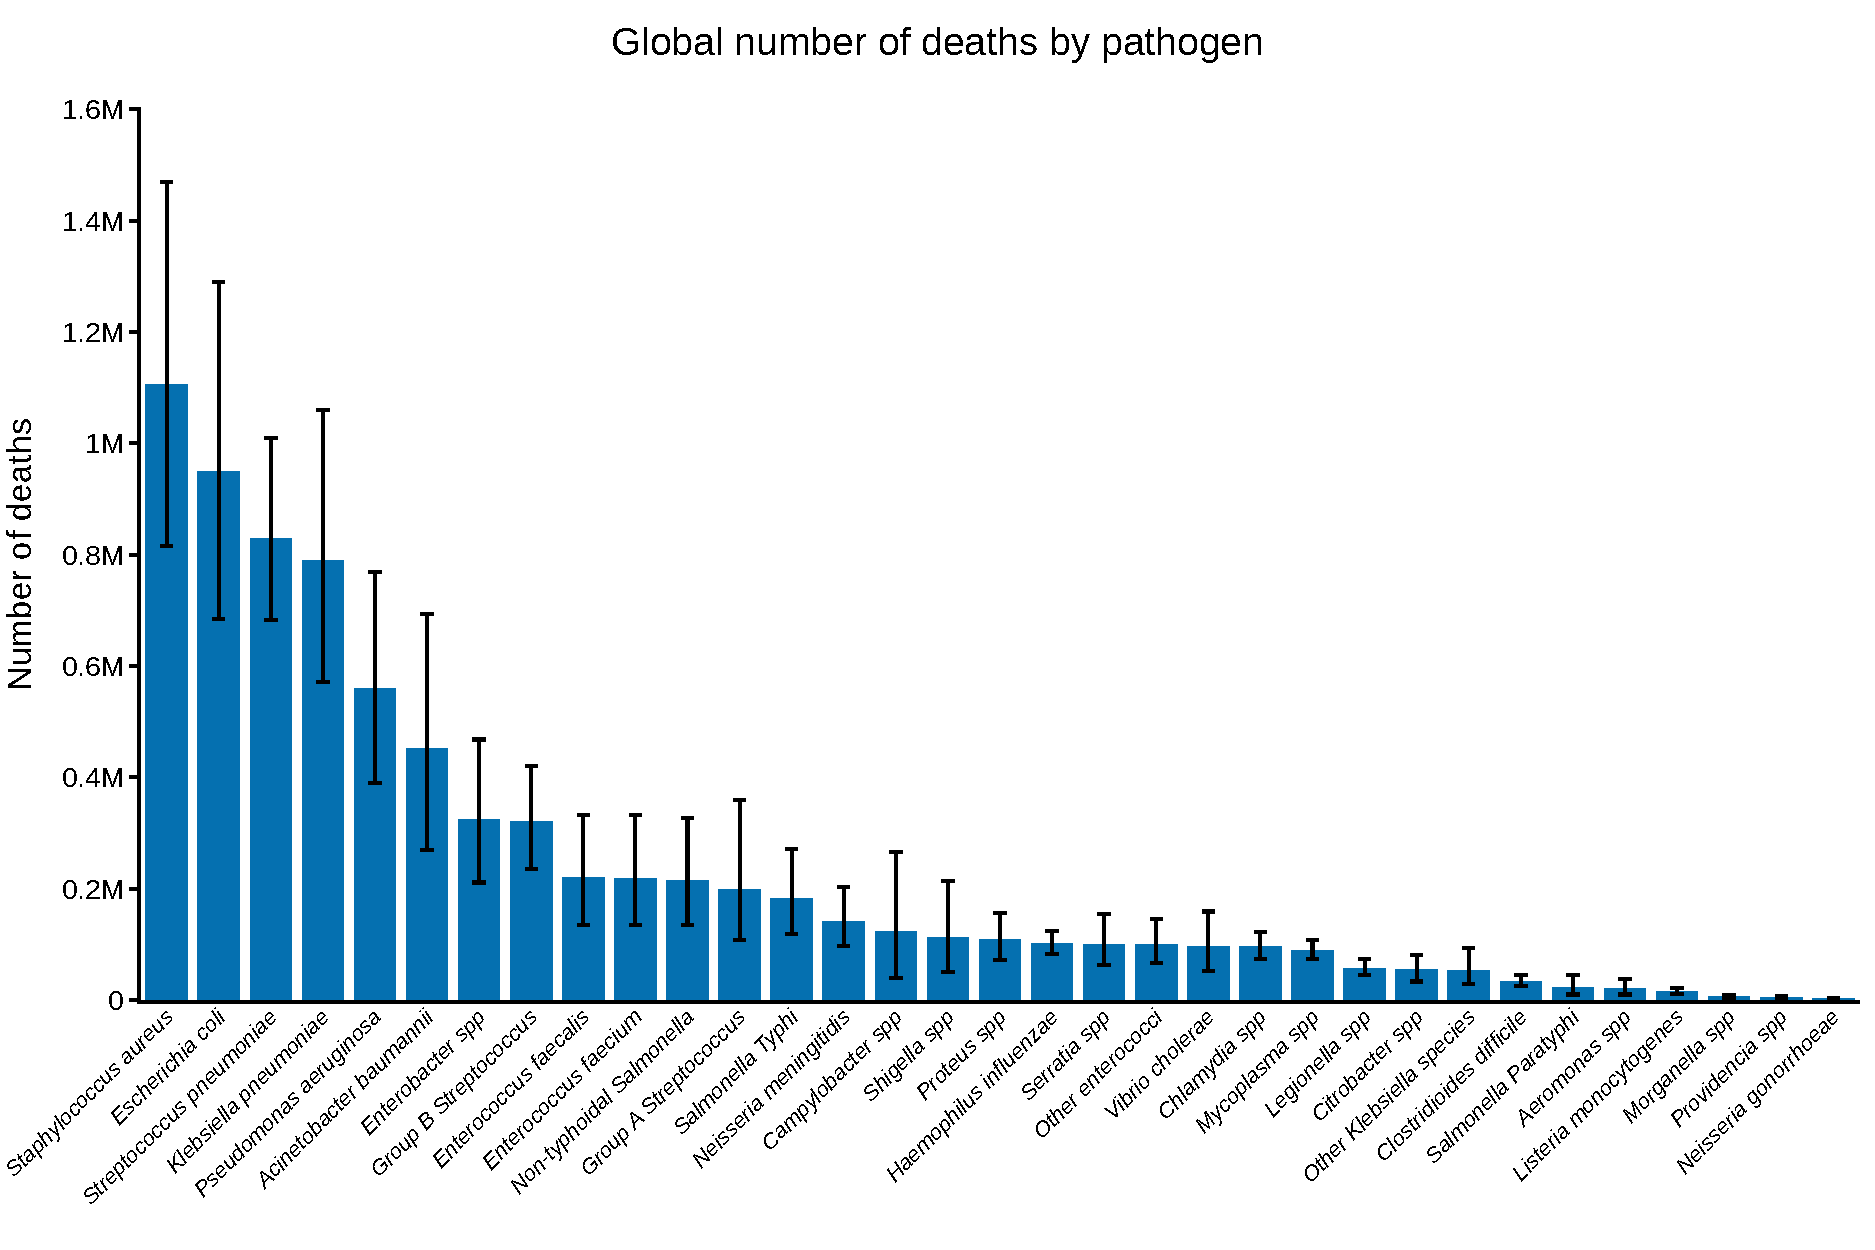
\includegraphics[angle=0,width=\textwidth]{figures/introduction/Figure1.pdf}
    \caption[Global number of deaths, in millions, associated to 33 bacterial pathogens in 2019]{Global number of deaths, in millions, associated to 33 bacterial pathogens in 2019. The error bars represent the 95\% uncertainty intervals. Adapted from \cite{ikuta_global_2022}.}
    \label{fig:introduction_figure1}
\end{figure*}

In the context of global mortality, these estimates put deaths associated with bacterial infections as responsible for at least 14\% of all global deaths \cite{ikuta_global_2022}. Moreover, the top five pathogens were associated with half of all bacterial deaths. These five pathogens are included in the \ac{WHO} \ac{BPPL} updated in 2024 \cite{noauthor_who_2024}. The \ac{BPPL} groups 15 families of antibiotic resistant pathogens into priority levels, with the aim of serving as a compass for \ac{RD} and for public health action. A global concerted effort of public health authorities is of the utmost importance to implement regionally tailored strategies to reduce the burden caused by bacterial infections. The implemented measures should combine infection prevention, vaccination, adequate methods of bacterial characterization and antibiotic usage, as well as promote \ac{RD} aiming to strengthen the resilience of these measures and future preparedness. Although all of these measures must be taken into account to develop effective strategies, the following sections will focus on common techniques used to characterize bacterial pathogens, with increasing emphasis on the application and impact of \ac{HTS} technologies and bioinformatics methods, steering us towards the objectives of this dissertation.

\begin{figure*}[!ht]
    \centering
    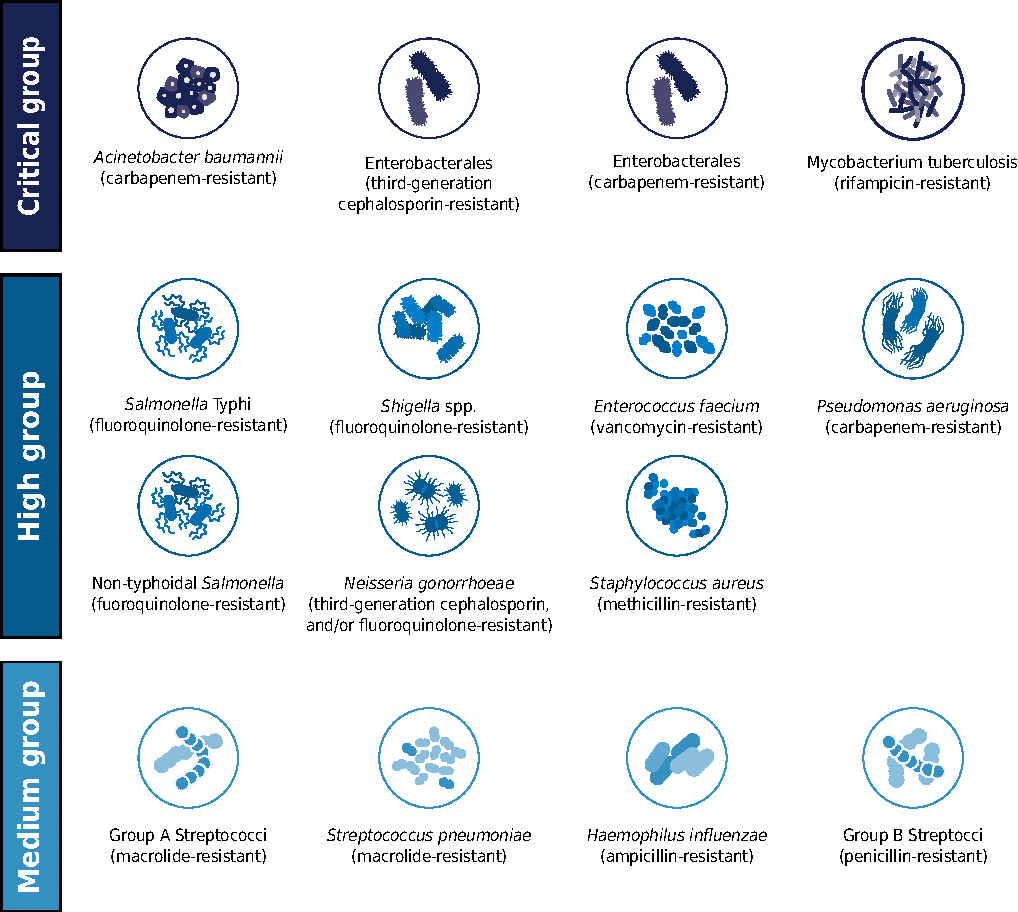
\includegraphics[angle=0,width=\textwidth]{figures/introduction/Figure2.pdf}
    \caption[\ac{WHO} Bacterial Priority Pathogens List, 2024 update]{WHO Bacterial Priority Pathogens List (BPPL), 2024 update. The \ac{BPPL} includes 15 families of \ac{ABR} pathogens, grouped into critical, high and medium categories of priority for \ac{RD} and for public health measures. Adapted from \cite{noauthor_who_2024}.}
    \label{fig:introduction_figure2}
\end{figure*}

\section{Bacterial characterization}

The characterization of pathogen samples is essential for the effective management of infected patients and the epidemiology of infectious diseases. Bacterial characterization or typing methodologies can be divided into phenotyping and genotyping \cite{li_bacterial_2009}. The former characterizes bacteria based on phenotypic assays, such as colony morphology on various culture media, biochemical tests, serology, and antibiotic susceptibility. The latter distinguishes bacteria on the basis of their genetic content and has been increasingly adopted to complement or substitute phenotypic assays. Genotyping allows inferring phenotypic characteristics through methods that are less complex and more broadly applicable than classical phenotypic assays, and in many cases has the potential to provide greater resolution. Microbiologists use both approaches to infer specific phenotypic characteristics, such as susceptibility to antimicrobial drugs, allowing to set the best course of action for patient treatment or mitigate the impact of an outbreak. Phenotypic assays rely on the expertise of clinical microbiologists who apply specialized and often species-specific techniques that were developed and optimized over years of research. These techniques involve complex and multi-step protocols that, depending on the bacterial species, can take less than a day or a few days (e.g. rapid-growing bacteria such as \textit{Escherichia coli} \cite{son_growth_2021}), to several weeks (e.g. slow-growing bacteria such as \textit{Mycobacterium tuberculosis} \cite{gordon_microbe_2018}) \cite{didelot_transforming_2012}. The application of \ac{HTS}, in combination with the development of specialized bioinformatics methods, has allowed researchers to reduce sample turnaround time by avoiding specific methodologies in favor of approaches such as \ac{WGS}, which allows to accurately identify the genomic features associated with the phenotypic characteristics of interest from sequence data to provide equivalent results to more laborious and time-consuming lab protocols. Notwithstanding the impact of the latest developments in sequencing technologies and bioinformatics methods, there is still no single method for bacterial characterization that is universally ideal, with each method having to strike a balance between several desired characteristics, such as being applicable to all isolates, highly discriminatory at all levels, generating reproducible results at intra- and inter-laboratory level, while also using modest resources.

\section{Phenotypic methods}

Classical bacteriology methodologies are based on successfully isolating a bacterial pathogen on culture media. Given that different bacterial species may have different growth requirements, microbiologists had to develop a wide repertoire of techniques to account for all the variable requirements. After successfully isolating a pathogen, microbiologists may perform a series of assays to determine, for example, the species of the pathogen and its antimicrobial and virulence profiles. The culture step varies according to the complexity of a sample. For samples from usually sterile sites, such as cerebrospinal fluid, it may be possible to report all organisms present in the sample and it is simpler to identify the ones that are clinically relevant and should go through further analysis steps. In the case of complex samples, such as faeces, isolating the \textit{micro culprit} may require a more custom approach guided by an educated guess about likely pathogens to select the appropriate media for culture and subsequent tests for a definitive diagnostic.

A correct species identification is highly informative, as it allows to deduce intrinsic characteristics from the body of knowledge and estimate the pathogenic potential, especially in the context of the isolation site. To identify the species of an isolate, microbiologists may use Gram staining, evaluate colony growth and morphology, and perform rapid biochemical tests, such as a bile solubility test, which is used to differentiate \textit{Streptococcus pneumoniae} from other alpha-hemolytic streptococci. Determining the biomolecule profiles of pure suspensions through \ac{MALDI-TOF} mass spectrometry and comparing them with known profiles is also used for rapid and cost-effective species identification, and to identify toxins and study bacterial antibiotic resistance \cite{croxatto_applications_2012, lasch_maldi-tof_2025, alizadeh_maldi-tof_2021, seng_ongoing_2009, idelevich_rapid_2018}.

Following culture and species identification, the determination of the antimicrobial resistance profile is crucial to select an effective treatment for infected patients. Antimicrobial resistance tests are mainly based on inhibition of \textit{in vitro} bacterial growth when exposed to an antibiotic. The efficacy of testing methods, such as disc diffusion and E-TEST, is compared against gold-standard susceptibility-testing systems, such as micro-dilution, to infer \textit{in vivo} efficacy.
The level of susceptibility to a given antibiotic is based on the \ac{MIC} and on the definition of \textit{breakpoints}, which correspond to the antibiotic concentration above which an isolate is considered to be resistant to therapy \cite{didelot_transforming_2012}. \textit{Breakpoints} are defined based on various factors that are not necessarily universally agreed upon, making it difficult to accurately compare and assess the efficacy of susceptibility testing and associate it with clinical outcome. Moreover, it is important to note that the results of susceptibility testing may not translate into similar \textit{in vivo} results, as resistance mechanisms may be more complex and depend on factors not adequately emulated by current susceptibility testing practices \cite{didelot_transforming_2012, hassall_limitations_2024}.

Compared to antimicrobial susceptibility testing, the detection of virulence factors tends to be overlooked when selecting an effective treatment for patients. Nonetheless, knowledge of the virulence profile of pathogens can play an important role when the presence of a virulence factor is known to contribute significantly to pathogenesis and disease severity. For example, toxin-producing strains of \textit{Clostridioides difficile} are more pathogenic and may require differential treatment. In public health, virulence factors are especially important as vaccine targets. For example, the variability of the capsule polysaccharide of \textit{Streptococcus pneumoniae} is detected by serotyping and the most relevant serotypes are targeted for vaccine development \cite{henrichsen_six_1995, tarrago_identification_2008, silva-costa_adult_2023, musher_remarkable_2022}. Serotyping is a good example of a phenotypic assay that is routinely applied and for which there are sequence-based genotyping alternatives, generally applied after \ac{WGS} to complement laboratory results or determine the serotype of strains of interest when only sequence data is available. In the case of \textit{S. pneumoniae}, \textit{in silico} serotyping is possible through specialized sequence databases\footnote{\url{https://www.pneumogen.net/gps/\#/serobank}} and software, such as SeroBA \cite{epping_seroba_2018, lorenz_serobav20_2025}. Another example is serotyping of \textit{Streptococcus pyogenes}, which measures the variability of the M protein, one of the targets of vaccine candidates in development \cite{walkinshaw_streptococcus_2023}. The \ac{CDC} hosts a database\footnote{\url{https://www.cdc.gov/strep-lab/php/group-a-strep/emm-typing.html}} with partial sequences of the M protein gene that is used by software such as emmtyper\footnote{\url{https://github.com/MDU-PHL/emmtyper}} for \textit{in silico} serotyping.

Although genotypic methods may be seen as viable substitutes for phenotypic methods, it is highly unlikely that a complete substitution will ever occur, especially for many of the major human pathogens for which phenotypic methods have been standardized and provide highly reliable and cost-effective results. Genotyping is relevant to complement these methods for diagnostic purposes and to provide greater resolution for applications such as research into mechanisms such as virulence and antimicrobial resistance. Genotyping may play a more dominant role for known or emerging pathogens and for the characterization of complex samples that cannot be well characterized with current phenotypic assays, opening the possibility of genotyping emerging as the gold standard in those cases.

\begin{figure*}[!ht]
    \centering
    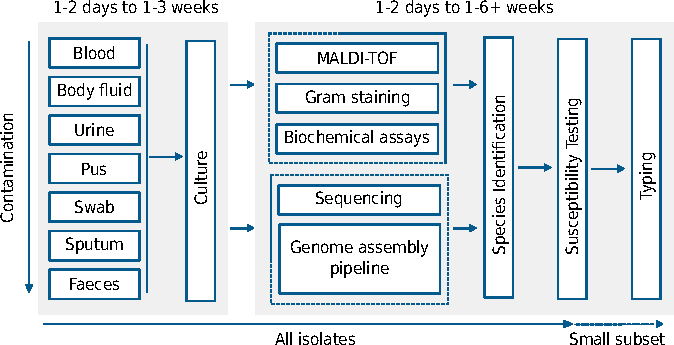
\includegraphics[angle=0,width=\textwidth]{figures/introduction/Figure3.pdf}
    \caption[Workflow representing typical steps in the processing of samples of bacterial pathogens.]{Workflow representing typical steps in the processing of samples of bacterial pathogens. Samples collected from normally sterile body sites are cultured on a rich medium with the necessary nutrients to support bacterial growth. For more complex samples, such as faeces, which may contain multiple bacterial species, selective media are used to favor the growth of the suspected pathogen. The growth of bacterial cultures can take from a day to several weeks depending on the growth requirements of the organism. After successful culture growth, methods such as \ac{MALDI-TOF}, gram staining and other biochemical assays can be used for species determination, followed by susceptibility testing. Depending on the species and the context of the infection, a small subset of the samples may be selected for further characterization using typing methods. Typing methods allow for a more detailed characterization of bacterial pathogens, which is especially useful in surveillance and outbreak investigation settings. DNA sequencing technologies are frequently used to substitute or complement lab-based approaches, allowing detailed characterization of bacterial pathogens through analysis of bacterial genomes with bioinformatics methods and providing faster turnaround times. Adapted from \cite{didelot_transforming_2012, mendes_towards_2023}}
    \label{fig:introduction_figure3}
\end{figure*}

\section{Genotypic methods}

With the introduction of molecular methods for bacterial characterization, the basis for systematics changed. The distinction based on classical phenotypic criteria was complemented or in part replaced by molecular criteria, particularly molecular sequences, because these methods can offer greater resolution, resulting in more precise phylogenetic analyses and diagnostics. Molecular methods can be divided into three main categories: i) \ac{DNA} banding pattern-; ii) \ac{DNA} hybridization-; and \ac{DNA} sequencing-based methods. The first differentiate bacterial strains based on the size and pattern of \ac{DNA} bands/fragments generated by \ac{DNA} amplification or cleavage of genomic \ac{DNA} using \ac{REs}. The second uses techniques such as \ac{DNA} macroarrays and microarrays, which distinguish strains through hybridization to probes complementary to known sequences. The third determine and compare the \ac{DNA} sequence of genomic regions of interest, often determinant for a particular feature, to discriminate bacterial strains based on sequence variation.

\subsection{DNA banding pattern-based methods}

\ac{DNA} banding pattern-based methods, either through amplification by \ac{PCR} or digestion with \ac{REs}, can provide accurate and quick results and are generalizable for characterizing strains of any bacterial species.

In this category of methods, one that allows to differentiate bacterial strains and has been widely applied in public health is \ac{PFGE}. \ac{PFGE} is an electrophoretic technique that applies alternating electric fields at different angles to separate large \ac{DNA} molecules ($10kb-10Mb$) \cite{schwartz_separation_1984, herschleb_pulsed-field_2007, lopez-canovas_pulsed_2019}. Prior to electrophoretic separation, \ac{REs} that recognize uncommon motifs are used to cleave the bacterial \ac{DNA}. The distinct banding patterns produced by \ac{PFGE} reflect the \ac{DNA} polymorphisms at the \ac{REs} recognition sites and, ideally, can be uniquely associated to a specific bacterial strain. The resolution of \ac{PFGE} depends on the choice of the \ac{REs} used, with \ac{REs} that recognize long and rare motifs yielding potentially more discriminatory results. The standardization of \ac{PFGE} protocols and the creation of pattern databases, such as the one hosted by Pulsenet International\footnote{\url{https://www.pulsenetinternational.org/protocols/pfge}}, were crucial to the wide adoption of \ac{PFGE}. Although widely used, \ac{PFGE} is laborious and the results can be influenced by multiple factors, which hinders reproducibility and interoperability \cite{li_bacterial_2009}. Due to these limitations and to the invention of \ac{HTS}, \ac{PFGE}, once considered the gold standard for bacterial typing \cite{neoh_pulsed-field_2019}, has gradually been replaced by more accurate and versatile methods based on \ac{WGS}, which allow a much more detailed and increasingly cost-effective characterization of bacterial strains based on the complete or nearly complete genome sequence.

Another method used to differentiate bacterial strains and infer relatedness is \ac{RFLP} \cite{thibodeau_use_1987, todd_chromosome_2001}. \ac{RFLP} allows to differentiate patterns of electrophoresis-separated restriction fragments by Southern Blotting with labeled probes \cite{southern_detection_1975}. The similarity of the patterns of \ac{RFs} is the basis for strain differentiation. Ribotyping is a variation of \ac{RFLP} that uses probes with conserved domains of \ac{rRNA} genes to differentiate strains based on variable regions flanking the bacterial \ac{rRNA} operons \cite{bingen_use_1994}. The distinct banding patterns identified through this approach are named ribotypes. Since \ac{rRNA} operons are universal, ribotyping is highly applicable. Furthermore, it generates fewer fragments that \ac{RFLP} approaches based on frequently cutting \ac{REs}, enabling easier interpretation of results and establishment of nomenclature and database systems. The potential cost-effectiveness of \ac{RFLP} can be overturned by time- and labor-consuming protocols, as well as the requirement for large amounts of high-quality \ac{DNA}, which is not always available. Ribotyping is an important method for the characterization and surveillance of \textit{Clostridioides difficile}, with some ribotypes associated with greater disease severity. To overcome the limitations of \ac{RFLP} specifically applied for ribotyping of \textit{C. difficile}, prediction directly from \ac{WGS} data can be performed with bioinformatics methods that estimate sequence similarity, such as sourmash \cite{moore_k-mer_2022, irber_sourmash_2024}, or using machine learning \cite{qi_p-224_2025}.

It would be unacceptable to move to the next category of molecular methods without mentioning the Swiss Army Knife of molecular biology: \ac{PCR}. The \ac{PCR} method, originally developed by Kary Mullis, allows the amplification of any target \ac{DNA} sequence in a sample in a cyclic process to generate a large number of copies of the target sequence \cite{mullis_specific_1986}. \ac{PCR} is performed by temperature cycling, with each cycle having three stages: denaturation, annealing, and elongation. Firstly, high temperature is applied during the denaturation stage to separate the \ac{DNA} strands. Secondly, the temperature is lowered to allow for the annealing of two oligonucleotide primers that flank the target sequence. Lastly, the temperature is raised to the optimum level at which a heat-stable polymerase can extend the primers by incorporating \ac{dNTPs}. Over the years, a plethora of \ac{PCR}-based methods were developed to expand the applicability and overcome limitations of the original \ac{PCR}, firmly establishing \ac{PCR} as one of the fundamental methods in molecular biology.
From the vast number of \ac{PCR}-based methods that were invented, some, such as multiplex \ac{PCR} and \ac{qPCR}, are broadly applicable. Multiplex \ac{PCR} uses multiple primer pairs to simultaneously amplify multiple target sequences in the same \ac{PCR} reaction \cite{chamberlain_deletion_1988}. \ac{qPCR} allows to simultaneously amplify target sequences and detect the \ac{PCR} product \cite{higuchi_simultaneous_1992, kubista_real-time_2006}. This is achieved by incorporating and monitoring the fluorescence of dyes or probes, which increases proportionally to the amount of product formed. \ac{qPCR} overcomes challenges related to product quantification in the original \ac{PCR} and allows for faster confirmation of the presence of a target sequence.
Other \ac{PCR}-based methods were developed for more specific tasks, such as genotyping. Methods such as \ac{AP-PCR or RAPD} \cite{welsh_fingerprinting_1990, williams_dna_1990}, which uses arbitrary primers for random amplification, and \ac{REP-PCR} \cite{versalovic_distribution_1991, de_bruijn_use_1992}, which amplifies regions between interspersed repetitive elements, generate fragment patterns that can function as signatures for specific bacterial strains. The identification of \ac{VNTR} in bacterial genomes through \ac{MLVA} enables to identify polymorphic sites \cite{lindstedt_multiple-locus_2005}. \ac{VNTR} elements evolve rapidly and the number of tandem repeats per locus may vary between strains. \ac{MLVA} uses \ac{PCR} to amplify multiple \ac{VNTR} loci, followed by analysis of the banding pattern to assign a genotype and infer phylogenetic relationships. Although \ac{MLVA} is a simple technique and may offer high resolution, \ac{VNTR} loci in closely related strains may evolve quickly, hindering long-term surveillance. Additionally, \ac{VNTR} may not be common in some species, which limits its applicability, and the accuracy of \ac{MLVA} might be affected by insertions or deletions in the amplified regions.
Some \ac{PCR}-based methods combine \ac{PCR} with other typing methods, such as methods that use \ac{REs}, to overcome limitations and improve accuracy. One example is \ac{PCR}-\ac{RFLP}, which can amplify target regions directly from clinical or environmental samples and uses \ac{REs} digestion of the \ac{PCR} amplicons to generate a limited number of \ac{RFs} that are more easily separated by gel electrophoresis and interpreted \cite{wichelhaus_rapid_2001}.
\ac{PCR}-based methods display multiple advantages, such as being relatively inexpensive, fast, and sensitive. Notwithstanding, researchers should be mindful about the inherent limitations of each \ac{PCR}-based method, and of limitations which are common to most \ac{PCR}-based methods, such as the potential for contamination, artifacts caused by, for example, non-specific amplification and primer dimerization, and the need for multiple controls. \ac{PCR} primer design is facilitated by tools such as Primer-BLAST\footnote{\url{https://www.ncbi.nlm.nih.gov/tools/primer-blast/}}, made freely available by the \ac{NCBI} \cite{ye_primer-blast_2012}. Multiple bioinformatics tools\footnote{\url{https://www.gear-genomics.com/silica/}}$^{,}$\footnote{\url{https://bigsdb.readthedocs.io/en/latest/data_analysis/in_silico_pcr.html}}$^{,}$\footnote{\url{https://ucsc.gao-lab.org/cgi-bin/hgPcr}} implement \ac{PCR}-like functionalities to search for sequences of interest based on flanking regions. \textit{In silico} \ac{PCR} is especially valuable to assess primer specificity in a range of applications and to identify highly variable regions whose detection is suboptimal with more common sequence comparison techniques such as alignment \cite{kalendar_silico_2024}.

\subsection{DNA hybridization-based methods}

\ac{DNA} hybridization-based methods use probes, which correspond to known \ac{DNA} fragments, to detect complementary \ac{DNA} sequences extracted from samples \cite{freeman_fundamentals_2000}. A variant of these methods uses \ac{DNA} arrays to test for the presence of hundreds to tens of thousands of \ac{DNA} fragments, being relevant for applications such as the study of the genetic diversity of bacteria and in transcriptomics. Two types of \ac{DNA} arrays exist: macroarrays \cite{gress_hybridization_1992, lennon_hybridization_1991} and microarrays \cite{derisi_use_1996, schena_quantitative_1995, shalon_dna_1996}. The former can contain up to five thousand spots, providing enough resolution to detect genes involved in \ac{AMR} or for typing methods based on the detection of polymorphisms in a smaller number of loci, such as spoligotyping for MTC bacteria. \ac{DNA} microarrays are more expensive, but provide far greater discriminatory power, including up to tens of thousands of distinct probes, enabling the identification of a greater number of loci compared to macroarrays or to study the variation at the genome or transcriptome level. Since the probes included in microarrays are defined based on reference sequences, microarrays may lack probes complementary to accessory genes, leading to an underestimation of genetic diversity. \ac{DNA} microarrays can use \ac{cDNA} or shorter oligonucleotides as probes. The former are used to determine gene presence, while the latter is capable of detecting smaller patterns of variation, such as deletions or even \ac{SNPs}. The use of \ac{DNA} arrays has largely been supplanted by the use of \ac{HTS} \cite{bumgarner_dna_2013}.

A \ac{DNA} hybridization-based method that has been applied to overcome some limitations of the classic culture-dependent approach is target capture through hybridization using oligonucleotide probes. In this approach, specialized bioinformatics software is used to design a set of probes to capture bacterial \ac{DNA} directly from clinical samples for subsequent \ac{HTS} \cite{dickson_probe_2021, chafin_mrbait_2018}. Bypassing the culture step is especially useful in reducing the turnaround time for fastidious bacteria such as \textit{M. tuberculosis} \cite{macedo_molecular_2023}, or to capture the \ac{DNA} of uncultivable bacteria, such as \textit{Treponema pallidum}, the causative agent of syphilis \cite{pinto_genome-scale_2016}. In addition, target capture has the potential to provide a less biased view of within-host variation by allowing to capture \ac{DNA} from multiple strains, contrasting with culture-dependent approaches, which may not meet the growth requirements of specific strains and often select a single colony from the culture plate for further characterization. In combination with \ac{HTS}, target capture allows culture-independent sequencing of clinical samples for faster diagnostics and detailed bacterial characterization. Designing probes to capture taxa at multiple taxonomic levels is also a powerful approach to study complex clinical samples and for metagenomics studies, allowing capture of known and related sequences and minimizing the obscuring effect of host \ac{DNA} abundance \cite{dickson_probe_2021}.

\subsection{DNA sequencing technologies}

The advent of \ac{DNA} sequencing technologies represented a major milestone in biological research, finally unlocking the genetic information encoded in \ac{DNA}, which had already been established as the source of genetic information in 1944 by Oswald Avery while working with \textit{Streptococcus pneumoniae} \cite{avery_studies_1944} and whose three-dimensional structure was determined in 1953 by Watson and Crick based on the crystallographic data produced by Rosalind Franklin and Maurice Wilkins \cite{watson_molecular_1953, zallen_despite_2003}. The potential and continuous improvement of these technologies contributed to their adoption and led to the development of highly reproducible and accurate methods used to differentiate bacterial strains and identify determinants of phenotypic features of interest. As sequencing throughput and sequence data availability increased, the diverse and highly dynamic nature of bacterial genomes was unveiled, leading to an unprecedented interest in developing sequence-based methods that could probe into the accumulated sequence data to gain new insights. The application of \ac{HTS} is revolutionizing our understanding of human health and disease by elucidating fundamental biological and ecological processes.

\subsubsection{First-generation DNA sequencing}

Sanger sequencing, also called dideoxy sequencing or chain termination \ac{DNA} sequencing, was the first generation of sequencing technologies \cite{sanger_dna_1977}. This method determines the nucleotide sequence of a single-stranded template \ac{DNA} using a \ac{DNA} polymerase to synthesize nucleotide fragments of different lengths by incorporating radio or fluorescently labeled \ac{ddNTPs} and through premature termination of the \ac{DNA} amplification elongation step \cite{heather_sequence_2016, rodriguez_genesis_2023}. The truncated fragments resulting from the interruption of the elongation step are size-separated by gel electrophoresis to reconstruct the original sequence. As the first successful \ac{DNA} sequencing technology, Sanger sequencing was instrumental in projects such as the sequencing of the first bacterial genome, the genome of \textit{Haemophilus influenzae} \cite{fleischmann_whole-genome_1995}, and the Human Genome Project, which in 2003 achieved the monumental task of determining the first nearly complete sequence of a human genome \cite{international_human_genome_sequencing_consortium_finishing_2004}.
Sanger sequencing was the most widely used sequencing technology until the newer and cheaper \ac{HTS} were developed.

\subsubsection{Second-generation DNA sequencing}

Pyrosequencing \cite{nyren_solid_1993, ronaghi_real-time_1996, margulies_genome_2005} was the first second generation \ac{SBS} technology to reach the market. The general principles of second generation \ac{SBS} technologies are the following: i) attachment of the \ac{DNA} to be sequenced to a solid support, usually combined with amplification to enhance signal detection; ii) single-stranded \ac{DNA} synthesis; iii) primer-dependent incorporation of complementary bases; iv) detection of each incorporated nucleotide for sequence determination. Pyrosequencing is based on real-time quantitative detection of pyrophosphate released as nucleotides are incorporated into a growing \ac{DNA} sequence, yielding reads around 400-500 \ac{bp} long. Initially, libraries of \ac{DNA} molecules are attached to paramagnetic beads via adapter sequences and amplified through emulsion \ac{PCR}. Ideally, on average only one \ac{DNA} molecule attaches to each bead so that each bead is coated in a clonal \ac{DNA} population after emulsion \ac{PCR}.

\begin{figure*}[h!]
    \centering
    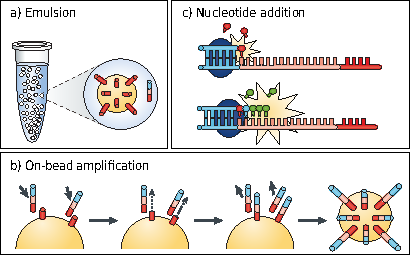
\includegraphics[angle=0,width=\textwidth]{figures/introduction/Figure4.pdf}
    \caption[454 pyrosequencing]{454 pyrosequencing. Fragmented DNA templates are amplified through emulsion \ac{PCR} (\textbf{a}), which consists on the hybridization of the DNA templates to bead-bound primers followed by amplification to cover each bead in thousands of copies of the same DNA sequence (\textbf{b}). The beads are arrayed onto a microtitre plate along with primers and different beads that contain enzymes. Sequencing occurs in cycles. In each cycle, a single nucleotide species is added and nucleotides are incorporated into growing chains by a DNA polymerase. When a base is incorporated, the release of an inorganic pyrophosphate triggers an enzyme cascade, resulting in light. Each burst of light is detected by a device to determine the bases incorporated at a particular bead (\textbf{c)}). Adapted from \cite{loman_twenty_2015, goodwin_coming_2016}}
    \label{fig:introduction_figure4}
\end{figure*}

The \ac{DNA}-coated beads are distributed into a plate that fits one bead per well where pyrosequencing occurs as bead-linked enzymes and \ac{dNTPs} are added and the pyrophosphate release is detected by a sensor \cite{heather_sequence_2016, nyren_history_2015, ronaghi_sequencing_1998, nyren_enzymatic_1987}. Compared to conventional Sanger sequencing, pyrosequencing has much higher throughput with a fraction of the cost, making it easier and more viable to scale-up. It does have some limitations over Sanger sequencing, however, as the read lengths are shorter, making downstream analysis, such as assembly, more complex. The most used pyrosequencing technology was 454 sequencing, which had major advantages over traditional Sanger sequencing, as demonstrated by its application to investigate drug resistance in \textit{Mycobacterium tuberculosis} \cite{andries_diarylquinoline_2005} and the whole genome sequencing of Jame Watson’s genome in record time and within a fraction of the cost of the Human Genome Project \cite{rothberg_development_2008, wheeler_complete_2008}. 454 sequencing was eventually discontinued in favor of more accurate and advanced technologies, such as Illumina’s \ac{SBS}.
Further improvements to massive parallel \ac{SBS} were introduced with the development of reversible and fluorescently labeled terminators \cite{turcatti_new_2008}. The most widely known sequencing strategy that incorporated these improvements is Illumina’s \ac{SBS} \cite{uhlen_sequential_2023, bentley_accurate_2008, fedurco_bta_2006}. Illumina’s \ac{SBS} systems enable \ac{MPS} of small \ac{DNA} fragments, yielding sequencing reads with up to 250 bp. Illumina’s \ac{SBS} technology starts by binding adapter sequences to the \ac{DNA} libraries, which contain complementary sequences that bind to the flow cell, unique indexes or barcodes for sample identification, and the sequencing primer binding sites. The \ac{DNA} molecules attached to the flow cell undergo bridge amplification to generate clonal clusters. Sequencing is performed in cycles by using ‘reversible-terminator’ \ac{dNTPs} and detecting the incorporated nucleotides before proceeding to the next cycle. After sequencing the forward strand in this manner, Illumina’s systems are capable of sequencing the reverse strand, generating \ac{PE} data, which significantly improves the accuracy of downstream analysis. The advantages of Illumina’s \ac{SBS} systems led to their worldwide adoption and establishment as the dominant sequencing technology for projects of any scale. The higher throughput of Illumina’s \ac{SBS}, especially as sequencing costs decreased, led to an explosion of sequence data, effectively pushing research into the era of \textit{big data} and data-driven research \cite{uhlen_sequential_2023}. The tremendous increase in the number of microbial genomes deposited in public databases in recent years is in great part due to the widespread application of second-generation sequencing technologies, especially of Illumina’s \ac{SBS}. Other examples of the successful application of this technology are the sequencing of 25,000 cancer genomes by the Cancer Genome Consortium \cite{zhang_international_2019} and the 100,000 Genomes Project \cite{the_100000_genomes_project_pilot_investigators_100000_2021}.

\begin{figure*}[h!]
    \centering
    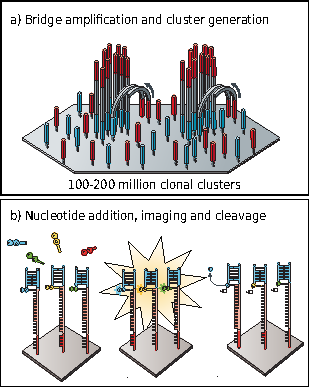
\includegraphics[angle=0,width=0.7\textwidth]{figures/introduction/Figure5.pdf}
    \caption[Illumina \ac{SBS}]{Illumina \ac{SBS}. In Illumina's SBS, DNA templates hybridize with adapters bound to a flow cell and are amplified though bridge-PCR to generate millions of clonal clusters (\textbf{a)}). In each cycle, fluorophore-labelled and terminally-blocked nucleotides are added and hybridize to complementary bases. Flow cells are imaged to measure the color of the emitted light when a base is incorporated (\textbf{b)}). Fluorophores are cleaved and washed before a new cycle begins. Adapted from \cite{loman_twenty_2015, goodwin_coming_2016}.}
    \label{fig:introduction_figure5}
\end{figure*}

\subsubsection{Third-generation DNA sequencing}

The third-generation of sequencing technologies provide single-molecule sequencing and eliminate the requirement of \ac{DNA} amplification characteristic of second-generation sequencing technologies. Currently, the most successful technologies are HiFi sequencing from \ac{PacBio} \cite{wenger_accurate_2019, eid_real-time_2009} and Nanopore sequencing from \ac{ONT} \cite{mikheyev_first_2014, stoddart_single-nucleotide_2009}. HiFi sequencing works by creating circularized \ac{DNA} libraries that are sequenced in repeated passes to generate several subreads per \ac{DNA} molecule, which can be compared to determine a consensus read minimizing sequencing errors. HiFi sequencing occurs inside small wells on a \ac{SMRT} Cell microchip where \ac{DNA} extension with fluorescent \ac{dNTPs} is finely monitored. The sequencing technology implemented by \ac{ONT} passes \ac{ssDNA} through a biological nanopore embedded in a synthetic membrane, across which a voltage is applied. The passage of the \ac{ssDNA} through the nanopore limits ionic flow and induces a current change for a period of time that allows to infer the sequence of the \ac{ssDNA} traversing the nanopore. Both technologies generate reads with length that can far exceed the length of the reads generated by second-generation technologies, which is why they are also called long-read technologies. With HiFi sequencing, read lengths can reach 1 to 25 \ac{kb}. Nanopore sequencing is capable of generating even longer reads, from a few to more than a hundred \ac{kb}. Accuracy-wise, HiFi sequencing has the high ground, but nanopore sequencing provides faster results and greater portability, crucial in outbreak investigation settings for fast pathogen detection and characterization. In addition, the development of new nanopores, base calling software, and experimental protocols tailored to particular applications has contributed to a gradual improvement in the accuracy of nanopore sequencing \cite{wang_nanopore_2021, wick_autocycler_2025, foster-nyarko_nanopore-only_2023, wick_trycycler_2021}. Despite continuous improvements in long-read sequencing technologies, their error rate is still higher than that of short-read sequencing technologies, such as Illumina's \ac{SBS}. For this reason, long- and short-read data have been used in combination to overcome limitations of both sequencing technologies and obtain higher-quality genome assemblies. When applied to the assembly of bacterial genomes, this strategy allows to assemble complete and error-free genomes, which cannot be achieved by using any of the technologies separately \cite{wick_assembling_2023, bouras_hybracter_2024, stevens_comparison_2023, wick_assembling_2023, bouras_hybracter_2024}.

\begin{figure*}[h!]
    \centering
    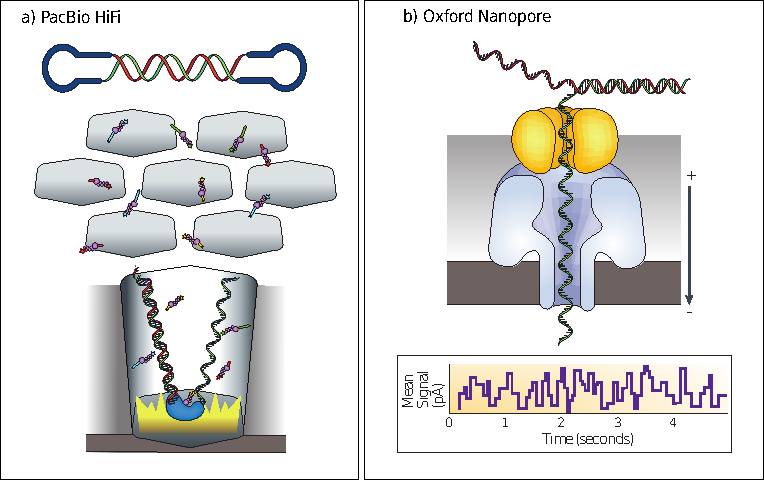
\includegraphics[angle=0,width=\textwidth]{figures/introduction/Figure6.pdf}
    \caption[PacBio HiFi and Oxford Nanopore sequencing]{PacBio HiFi (\textbf{a}) and Oxford Nanopore sequencing (\textbf{b)}). In HiFi sequencing, two hairpin adapters are added to the DNA templates to allow for continuous circular sequencing. HiFi sequencing occurs inside wells where labelled dNTPs are incorporated and a camera records the emitted light. Nanopore sequencing adds a hairpin and a leader adapter to DNA templates. The leader adapter interacts with a motor protein and a biological nanopore, directing the DNA into the pore. As the DNA translocates the pore, a shift in voltage is measured to determine the composition of the DNA sequences. Adapted from \cite{loman_twenty_2015, goodwin_coming_2016, wang_nanopore_2021, metzker_sequencing_2010}.}
    \label{fig:introduction_figure6}
\end{figure*}

\subsection{DNA sequencing-based methods}

As \ac{HTS} technologies became more accurate and cost-effective, wide adoption by research and public health institutions became a possibility. The application of these technologies to help resolve infectious disease events, such as the cholera epidemic in Haiti after the 2010 earthquake \cite{barzilay_cholera_2013} and the international outbreak of \textit{Escherichia coli} disease linked to contaminated fenugreek sprouts \cite{king_outbreak_2012, mellmann_prospective_2011}, quickly revealed that they were an invaluable tool for the surveillance and outbreak investigation of bacterial pathogens. \ac{WGS} of bacterial isolates, performed with second or third generation sequencing technologies, followed by genome assembly, allows the determination of the complete or nearly complete genome sequence, which in principle encodes most of the genetic features necessary for a detailed characterization of an isolate. Genome assembly is performed with pipelines such as Shovill\footnote{\url{https://github.com/tseemann/shovill}}, INNUca\footnote{\url{https://github.com/B-UMMI/INNUca}} \cite{prjibelski_using_2020, walker_pilon_2014, bolger_trimmomatic_2014}, and Bactopia\footnote{\url{https://github.com/bactopia/bactopia}} \cite{petit_bactopia_2020}, typically based on a \textit{de novo} approach to determine a set of contiguous sequences, called \textit{contigs}, resulting from the comparison and combination of overlapping sequencing reads. The application of specialized bioinformatics software allows identifying the relevant features for typing and diagnosis based solely on a sequence approach, complementing or replacing traditional microbiological workflows \cite{besser_next-generation_2018, deurenberg_application_2017}. Moreover, \ac{WGS} may also allow for the identification of emerging genetic features not tested for in routine molecular tests and the detection of uncultivable bacterial strains \cite{deurenberg_application_2017}.

The surveillance of food-borne diseases has greatly benefited from the implementation of standardized \ac{WGS}-based systems. An estimated 600 million people fall ill due to contaminated food annually, resulting in over 400 thousand premature deaths \cite{noauthor_who_nodate}. This puts global public health systems under strain and leads to significant costs related to medical treatment and to productivity and trade losses. Initial reports on the adoption of \ac{WGS} by the PulseNet surveillance network in 2000 demonstrated improved outbreak detection and an increase in the number of solved outbreaks compared to using \ac{PFGE} data \cite{besser_next-generation_2018, jackson_implementation_2016, ribot_pulsenet_2019}. The gradual adoption of \ac{WGS} by the network participants and the standardization of analytical workflows established \ac{WGS} as the gold standard for typing of foodborne pathogens tracked by the network. In 2019, the \ac{ECDC} published a strategic framework for the integration of molecular and genomic typing into European surveillance and multi-country outbreak investigation \cite{european_centre_for_disease_prevention_and_control_ecdc_2019}. The document included a progress report on the implementation of \ac{WGS} for surveillance and outbreak investigations by the \ac{EU/EEA} member states and outlined key technological milestones to improve the surveillance and outbreak detection of priority pathogens/diseases. Joint work of the \ac{ECDC} and \ac{EFSA} resulted in the implementation of the \ac{EFSA} and \ac{ECDC} One Health \ac{WGS} System, which aims to augment surveillance capacity and coordination among \ac{EU/EEA} member states \cite{authority_efsa_guidelines_2022}. This system has been instrumental in detecting and resolving multiple multi-country outbreaks \cite{noauthor_prolonged_2024, authority_prolonged_2024, european_centre_for_disease_prevention_and_control_european_food_safety_authority_multi-country_2023, european_centre_for_disease_prevention_and_control_european_food_safety_authority_multi-country_2022}.

Building \ac{WGS} capacity requires significant investment in sequencing instruments, reagents, and computational resources to store and analyze \ac{WGS} data. The choice of analytical methods is crucial and may be especially complex as there are multiple fundamental approaches which are not necessarily equivalent or comparable \cite{mixao_multi-country_2025}. Multiple bioinformatics methods have been developed for the detailed characterization of bacterial strains. Some methods characterize strains based on the identification of a single locus, such as \textit{in silico} serotyping or abundance estimation based on the 16S \ac{rRNA} gene. Other methods offer greater resolution by identifying and measuring the variability of a greater number of loci, such as \ac{GbG}, \ac{SNP}-based, and \textit{k}-mer-based methods. These methods have been increasingly integrated into \ac{WGS}-based systems for surveillance, outbreak investigation, and the study of bacterial populations. For this reason and because of their superior potential for further improvement, they are more relevant to the work developed in this dissertation, and a greater focus is given to these methods in the following sections.

\subsubsection{Multilocus sequence typing}

\ac{MLST} is a sequence-based approach that uses allele fragments, typically seven, from housekeeping genes to characterize microorganisms, with a more expressive application for bacterial species of pathogenic potential. \ac{MLST} is based on the principles of \ac{MLEE}, but uses nucleotide sequences at each locus, taking advantage of developments in sequencing technologies and bioinformatics \cite{urwin_multi-locus_2003}. Moreover, \ac{MLST} allows identifying a larger number of alleles per locus, offering higher discrimination than \ac{MLEE} while using a smaller number of loci. \ac{MLST} was initially developed to better accommodate vertical and horizontal genetic transfer signals and overcome the challenges of traditional and molecular typing methods, such as the inability to infer strain relatedness and poor reproducibility within and between laboratories \cite{maiden_multilocus_1998}.

\begin{figure*}[h!]
    \centering
    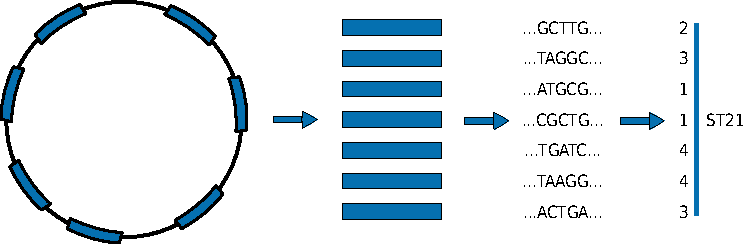
\includegraphics[angle=0,width=\textwidth]{figures/introduction/Figure7.pdf}
    \caption[Multilocus Sequence Typing]{Multilocus Sequence Typing (MLST). In \ac{MLST}, the internal fragments of a set of housekeeping genes, typically seven, are amplified through \ac{PCR} and sequenced. Each distinct sequence is assigned an allele identifier, and the combination of allele identifiers constitutes an allelic profile. Each distinct allelic profile is assigned a \ac{ST}, which allows to identify groups of similar strains.}
    \label{fig:introduction_figure7}
\end{figure*}

The distinct fragments identified at each locus are assigned unique integer identifiers in order of discovery, and the combination of identifiers for the allele fragments identified in all loci constitutes an allelic profile, which can be compared against a database of known allelic profiles. Each distinct allelic profile unambiguously defines a \ac{ST}, assigned to isolates for direct comparisons. \ac{ST}s are grouped into \ac{CC}, a concept first introduced to describe \textit{N. meningitidis} isolates analyzed by \ac{MLEE}, based on their similarity to a central \ac{ST} (allelic profile or genotype). The definition of central \ac{ST}s is achieved through a combination of computational and experimental data obtained from public health authorities. Newly identified \ac{ST}s are assigned to the most similar \ac{CC} based on a minimum number of shared alleles with the central \ac{ST}. \ac{ST} organization into \ac{CC}s facilitates epidemiological analysis, often grouping most \ac{ST}s into a much smaller number of \ac{CC}s and allowing to identify \ac{CC}s of greater clinical relevance. One disadvantage of \ac{MLST} is that it may not offer the same degree of discrimination within lineages or species with highly uniform housekeeping genes. Furthermore, due to the diversity of bacterial species, \ac{MLST} schemes must be developed to distinguish closely related bacteria, usually at the genus and species levels, or they may not provide sufficient resolution. Consequently, \ac{MLST} cannot be applied as a combined taxonomic and typing approach at all levels of bacterial diversity \cite{jolley_ribosomal_2012}.

By relying on the sequencing of allele fragments from multiple chromosomal locations, \ac{MLST} provides unambiguous results and is more robust to recombination events, constituting a faster and more sensitive technique than most laborious lab protocols, which also tend to be more unpredictable as variation accumulates. Since allele fragments are used as a unit of comparison, single allele differences constitute a single event, regardless of the number of nucleotide polymorphisms involved. While this model may not provide resolution for every single point change, it is resistant to horizontal genetic transfer events, which introduce a lot of variation in a single event, leading to an inaccurate estimate of similarity if counted as single differences. \ac{MLST} aims to provide good discrimination for short- and long-term epidemiology. The original study showed that it was congruent and more discriminatory than \ac{MLEE} in distinguishing hyper-virulent strains of \textit{Neisseria meningitidis} while also offering a clear distinction between lineages at the species level. A subsequent study presented a \ac{MLST} database for \textit{Streptococcus pneumoniae}, obtaining consistent results with \ac{MLEE} and \ac{PFGE} for the analysis of predominantly invasive and antibiotic-resistant isolates. Moreover, \ac{MLST} was also congruent with serotyping, with isolates that share the same or similar \ac{ST}s also expressing the same serotype, except for cases where recombination at the capsular locus was suspected to have led to capsular switching \cite{enright_multilocus_1999}.

Numerous \ac{MLST} databases have been developed since \ac{MLST} was proposed. Currently, a public collection of curated and frequently updated \ac{MLST} databases is available for a great number of microbial species on the PubMLST website\footnote{\url{https://pubmlst.org/}}. PubMLST integrates sequence data with sample metadata to promote the exchange of molecular typing data for epidemiological studies. As of 27 March 2025, PubMLST manages more than 130 species and genera-specific \ac{MLST} databases, which contain tens of millions of alleles identified and submitted by researchers. The sheer volume of data and the range of databases in PubMLST highlight how the advantages of \ac{MLST} contributed to its rapid adoption worldwide, with the technique widely used for epidemiological studies, to identify localized disease outbreaks and monitor local and global trends, and for population studies, to examine the structure of bacterial populations and perform evolutionary analyzes.

\subsubsection{rMLST}

\ac{rMLST} typing indexes the variation of the genes encoding the bacterial \ac{rps}. The \ac{rps} genes are ideal targets for universal bacterial characterization because they are: i) universally present; ii) distributed across the genome, which makes \ac{rMLST} more robust against horizontal gene transfer events that reassort loci and break phylogenetic congruence; and iii) encode proteins which are functionally conserved across the Bacteria domain. \ac{rMLST} constitutes a combined taxonomic and typing approach for the whole domain of Bacteria at all taxonomic levels. \ac{rMLST} allelic profiles or \ac{rSTs} determined through \ac{rMLST} provide a basis for universal bacterial systematics, allowing for a precise identification of the phylogenetic position at any taxonomic rank, while also distinguishing closely-related strains for typing purposes. A database for the 53 \ac{rps} genes identified in bacteria is managed by the \ac{BIGSdb} platform \cite{maiden_mlst_2013}.

\subsubsection{wg/cgMLST}

The level of resolution for typing depends on the desired application. Higher resolution is necessary for the detection of outbreaks and within-patient variation. On the other hand, lower resolution is required to group strains into \ac{CC}s or lineages. The \ac{GbG} approach is inherently hierarchical and scalable, meaning that the number of genes used in the analyzes can be adjusted based on the desired resolution \cite{maiden_mlst_2013}. Thus, the concept and analysis methods of the highly successful seven-gene \ac{MLST} can be intuitively scaled to hundreds or thousands of genes to encompass diversity at the core- or whole-genome level, giving rise to \ac{wg/cgMLST}. \ac{wg/cgMLST} provides higher resolution for surveillance and outbreak investigation. Furthermore, the additive nature of \ac{MLST}, through the continuous update of schemas with novel alleles, ensures that \ac{wg/cgMLST} can provide accurate results in the long-term while also promoting interoperability.

\begin{figure*}[h!]
    \centering
    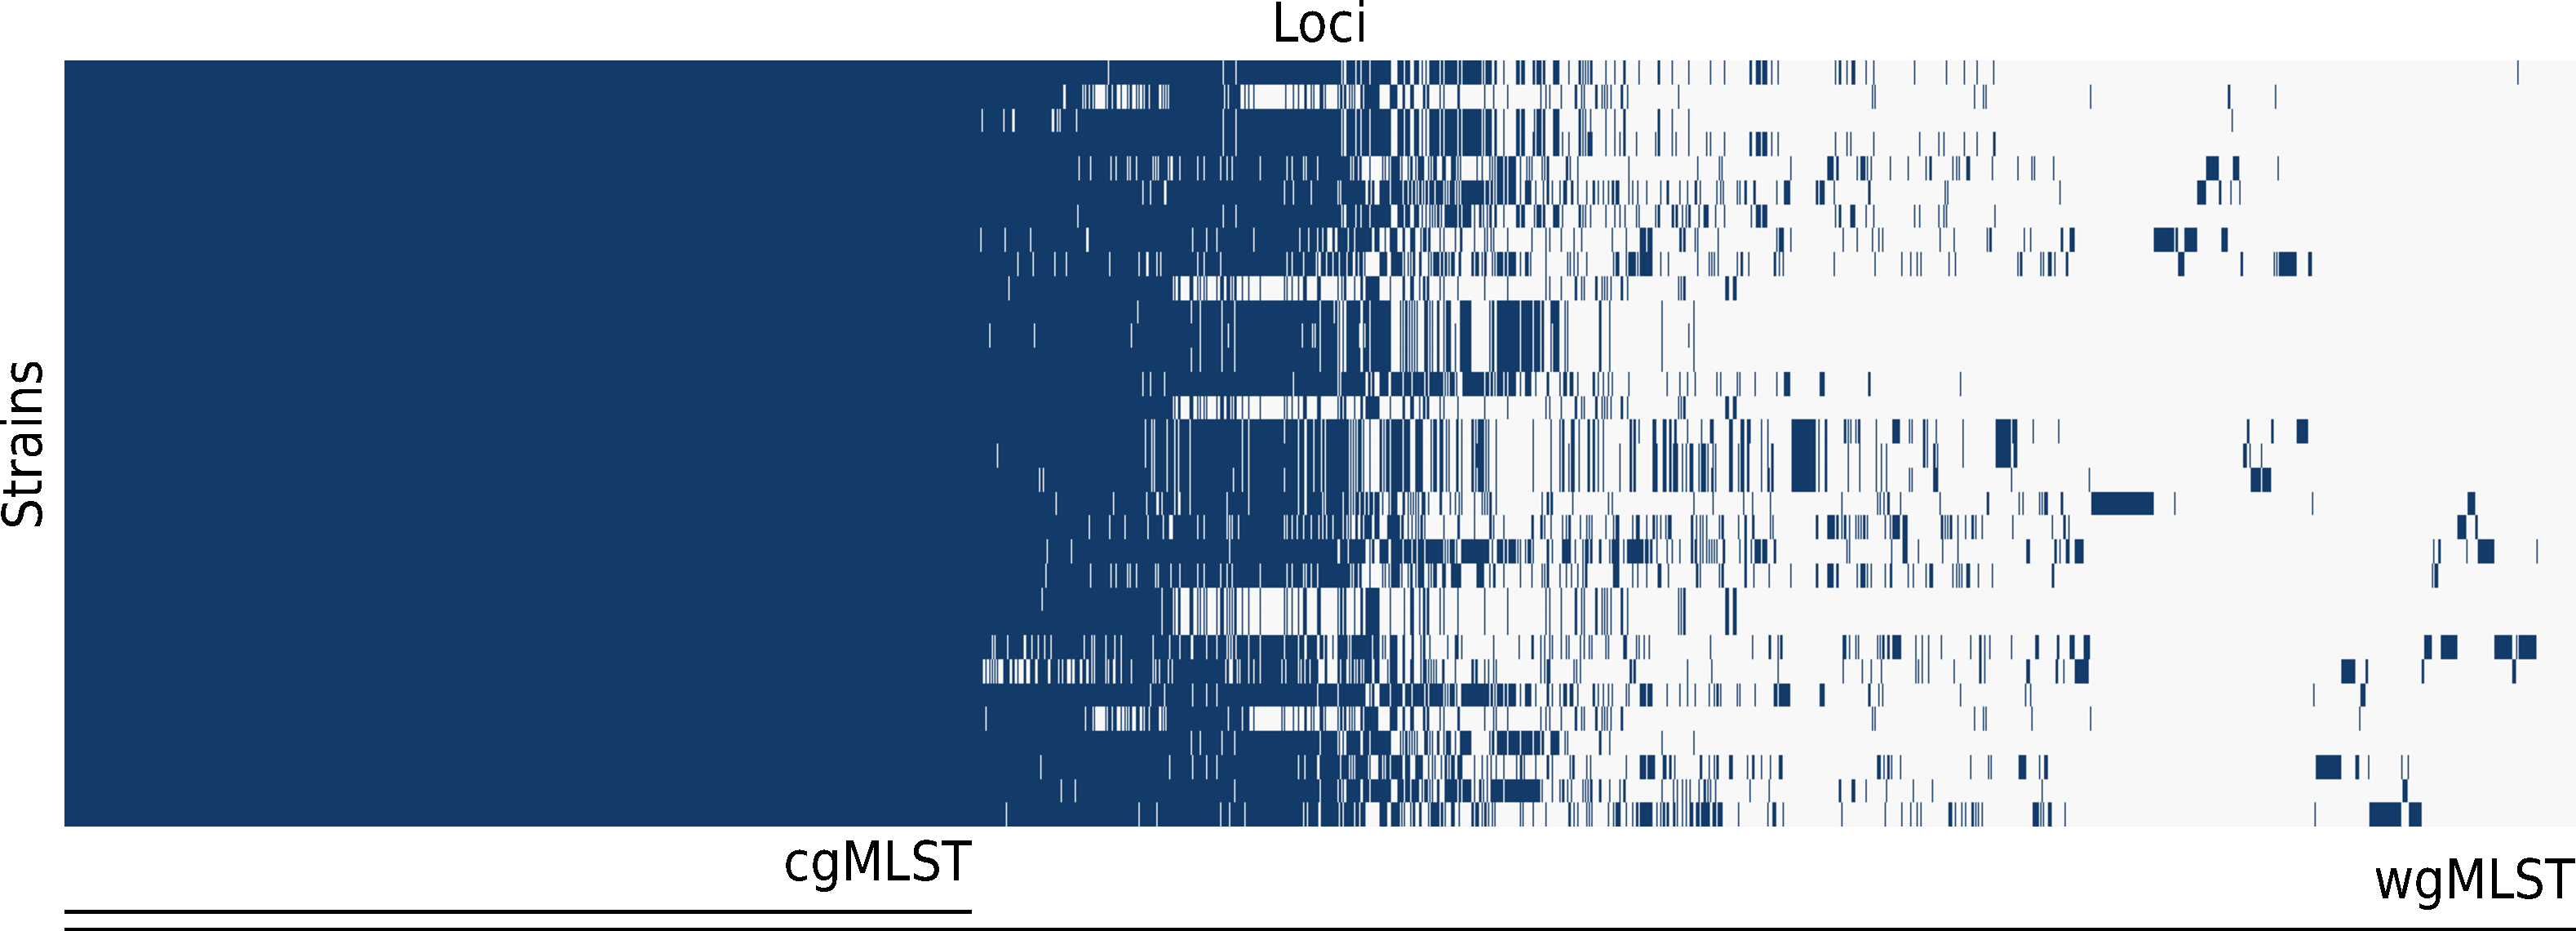
\includegraphics[angle=0,width=\textwidth]{figures/introduction/Figure8.pdf}
    \caption[Whole- and core-genome MLST]{Whole- and core-genome \ac{MLST} (\ac{wg/cgMLST}). The heatmap represents a presence-absence matrix of the loci (columns) in a wgMLST schema that were identified in 32 bacterial strains (rows). Darker regions indicate that a locus was identified in a strain, while lighter regions indicate locus absence. \ac{cgMLST} compares the set of alleles for the loci present in all strains (shorter line below the heatmap), while \ac{wgMLST} incorporates loci from the accessory genome (longer line below the heatmap).}
    \label{fig:introduction_figure8}
\end{figure*}

\ac{cgMLST} characterizes bacterial strains based on the identification and comparison of the genes that constitute the core genome. Although the core genome is often defined as the set of genes present in all strains of a given dataset, a more relaxed definition is needed to account for technical and biological variation. A loci presence threshold of 95\% is commonly used to accommodate biases and errors introduced by, for example, the sequencing and genome assembly processes. This allows to retain genes that are present in almost all strains of a species or that are reported as absent due to misassembly. Furthermore, the set of core loci is usually determined based on the allele calling results for a specific dataset ideally representative of the diversity of the species. This means that the definition of core genome is highly dependent on the dataset used and the number of core loci detected varies according to the dataset.

\ac{wgMLST} further expands the set of loci used for strain typing by including loci from the accessory genome. The frequency of accessory loci is highly variable, with some accessory loci being nearly as frequent as core loci, and others being found only in a small subset of strains or even being strain-specific. In theory, a \ac{wgMLST} schema should contain more loci than a \ac{cgMLST} schema, but there are no hard requirements regarding the fraction of core and accessory loci of a species that should be included, allowing for \ac{wgMLST} schemas with a number of loci close to that of a \ac{cgMLST} schema or considerably larger \ac{wgMLST} schemas encompassing all known core and accessory loci for a species. Since \ac{wgMLST} identifies more loci than \ac{cgMLST}, it provides greater resolution and is potentially more discriminatory when there is variation in the accessory genome. However, creating \ac{wgMLST} schemas requires a more careful selection of target loci compared to \ac{cgMLST} schemas. While \ac{cgMLST} schemas include only core loci, which usually display lower allele diversity, the inclusion of accessory loci in \ac{wgMLST} schemas increases the frequency of spurious loci due to sequencing and assembly errors or real sequence variability, affecting the accuracy of the results. Since \ac{cgMLST} provides robust results and most of the available schemas are \ac{cgMLST} schemas, most analyses are performed at that level, with \ac{wgMLST} being recommended when higher resolution is necessary, such as when comparing closely related strains for surveillance and outbreak detection \cite{mixao_multi-country_2025, joseph_evaluation_2023, leeper_evaluation_2023, leeper_validation_2025}.

\ac{wg/cgMLST} characterizes strains by determining their allelic profiles (i.e., the set of loci and alleles identified in each strain). The comparison of the allelic profiles to determine the number of shared loci and alleles provides an estimate of strain similarity. This can be done by discarding missing loci from the analysis or by computing the absolute difference. The former is preferred, as genome fragmentation and potential sequencing and assembly errors make it impossible to be certain if a locus that was not identified is in fact absent from the genome. The cross-comparison of a set of samples allows to compute a distance matrix including the number of allelic differences between each pair of strains. The distance matrix enables phylogenetic analysis through methods such as single-linkage clustering, \ac{NJ} or by computing a \ac{MST}. Computing a \ac{MST} is frequently used in surveillance and outbreak investigation scenarios as it provides accurate results when comparing closely related strains. For the study of more diverse populations, more robust results can be obtained using methods such as maximum likelihood after computing a \ac{MSA} for the alleles identified in all strains for each locus and concatenating the loci \ac{MSA}a to obtain a core genome \ac{MSA}. Multiple software and web platforms provide functionalities to generate and visualize trees from \ac{wg/cgMLST} results, including options to overlay the tree with metadata to more easily identify relevant strains. A distance threshold can be defined to identify groups of highly similar strains corresponding to lineages or potential outbreaks. Threshold definition is often empirical, depending on the diversity of the species, dataset, context, and methods used for the analysis. Consequently, threshold values are not universally applicable, which hinders comparability of the results obtained in different settings (e.g., outbreak detection in different countries.

\paragraph{wg/cgMLST platforms} \mbox{}\\

There are multiple web platforms that store and manage \ac{wg/cgMLST} schemas. These platforms provide access to \ac{wg/cgMLST} schemas for a wide range of species and offer different functionalities for data analysis. All well-established \ac{wg/cgMLST} platforms centralize data analysis by requiring users to upload their data. Platforms such as \ac{BIGSdb}\footnote{\url{https://pubmlst.org/software/bigsdb}} and Enterobase\footnote{\url{https://enterobase.warwick.ac.uk/}} operate under more permissive licenses, providing wide-access to schemas and functionalities upon registration and allowing other users or institutions to set up their own instances of the platform. Other platforms, such as Ridom SeqShere+\footnote{\url{https://www.ridom.de/seqsphere/}}, are proprietary software that requires users to pay for access to the platform's functionalities, although schemas used within the platform are publicly available. The results generated within different platforms are not directly comparable, as schemas for the same species stored by different platforms may target different sets of loci and use distinct loci and allele nomenclatures, which hinders interoperability. The results are not easily comparable even when the schemas have the same origin and use the same nomenclature, since each platform applies different methods for allele identification and the nomenclatures are not synchronized, which means that different identifiers can be assigned to the same allele depending on the platform.

\ac{BIGSdb} was the first platform to enable \ac{wg/cgMLST} and is a prime example of a solution for \ac{wg/cgMLST} that has been widely adopted and offers extensive analytical capabilities. \ac{BIGSdb} extended the functionalities for \ac{MLST} of the PubMLST platform to \ac{WGS} data \cite{jolley_bigsdb_2010, jolley_open-access_2018}. \ac{BIGSdb} pioneered the application of \ac{GbG} methods to genome analysis, storing genomic and gene sequences, as well as associated metadata, such as provenance and phenotypic data for isolates from which the sequence data originated. Additionally, it stores allele and locus definitions, without an inherent limit to the number of records or the number of schemas into which the loci can be grouped. The loci included in a schema do not need to be associated with a single organism, enabling the creation of schemas that encompass the diversity of genes, such as accessory genes, that are distributed in diverse organisms. Known and novel alleles are identified from sequence data uploaded to \ac{BIGSdb} to maintain a record of the known diversity of genes identified in the samples stored in the database. Furthermore, genomic data are periodically rescanned as the database expands to identify variants in stored isolates that could not be detected previously based on the represented allele diversity in the database. The functionalities included in \ac{BIGSdb} allow users to link isolate and sequence data with great flexibility, allowing the definition of schemas encompassing the diversity of species with utility for epidemiological investigations and population analysis or smaller schemas to study particular aspects of the biology of an organism. The genetic nomenclatures established and maintained by \ac{BIGSdb} enable the definition of classification hierarchies for an effective comparison of bacterial isolates globally \cite{jolley_open-access_2018}.

\subsubsection{SNP-based methods}

An accurate estimation of strain similarity for phylogenetic analyzes can be achieved by comparing the genomes of strains of interest against the genome of a reference strain to identify \ac{SNPs}. This is performed by mapping sequencing reads against a reference genome to identify all variable positions in regions shared with the reference, identifying the set of core \ac{SNP}s. Similarly to \ac{wg/cgMLST}, pairwise \ac{SNP} distances or the alignment of the core \ac{SNP}s can be determined to perform phylogenetic analysis with methods such \ac{NJ} or maximum likelihood, respectively. Since \ac{SNP}-based approaches identify variation at the single nucleotide level, they can potentially provide higher resolution than \ac{wg/cgMLST} for the regions being considered. However, it is necessary to meet two requirements for high-resolution typing with \ac{SNP}-based methods. First, choosing a reference genome closely related to the strains under investigation is of the utmost importance, as \ac{SNP}s are only identified in the regions shared with the reference. A more divergent strain may considerably reduce the number of shared regions, and consequently the number of detected \ac{SNP}s. Strategies for choosing a reference genome include selecting a high quality genome from the same \ac{ST}, \ac{CC}, serogroup or determining the genome distance to a group of candidate reference genomes to select the most appropriate. Second, the group of strains under investigation cannot be very diverse, as that will also reduce the number of regions considered for \ac{SNP} determination \cite{jolley_bigsdb_2010}. These requirements can be met for outbreak detection and investigation scenarios in which \ac{SNP}-based methods have been successfully applied to resolve national and international outbreaks. However, these requirements limit the applicability of \ac{SNP}-based methods compared to \ac{wg/cgMLST} approaches, which can be used to characterize from very diverse datasets to closely related strains. In addition, \ac{SNP}-based methods are less robust to recombination and \ac{HGT} than \ac{wg/cgMLST}, as a single event will lead to the identification of multiple \ac{SNP}s, potentially overestimating the distance between strains. The congruence between \ac{SNP}-based and \ac{wg/cgMLST} approaches is highly dependent on the reference genome and the schema used, respectively, as well as the parameters used and the dataset under analysis. While some studies have reported good congruence between both approaches for outbreak analyses, others have highlighted that the results are not directly comparable and that a congruence analysis is necessary to assess method equivalence \cite{mixao_multi-country_2025}. Furthermore, \ac{SNP}-based approaches do not scale as well as \ac{wg/cgMLST}, in part because they are more computationally demanding as the size of the dataset increases, but also because it may be necessary to use multiple references and fine-tune the parameters for accurate \ac{SNP} detection, making it harder to standardize or establish a reference database for consistent results. Nevertheless, variant calling data can be stored to promote reproducibility and minimize scalability concerns, an approach implemented in SnapperDB \cite{dallman_snapperdb_2018}.

\begin{figure*}[h!]
    \centering
    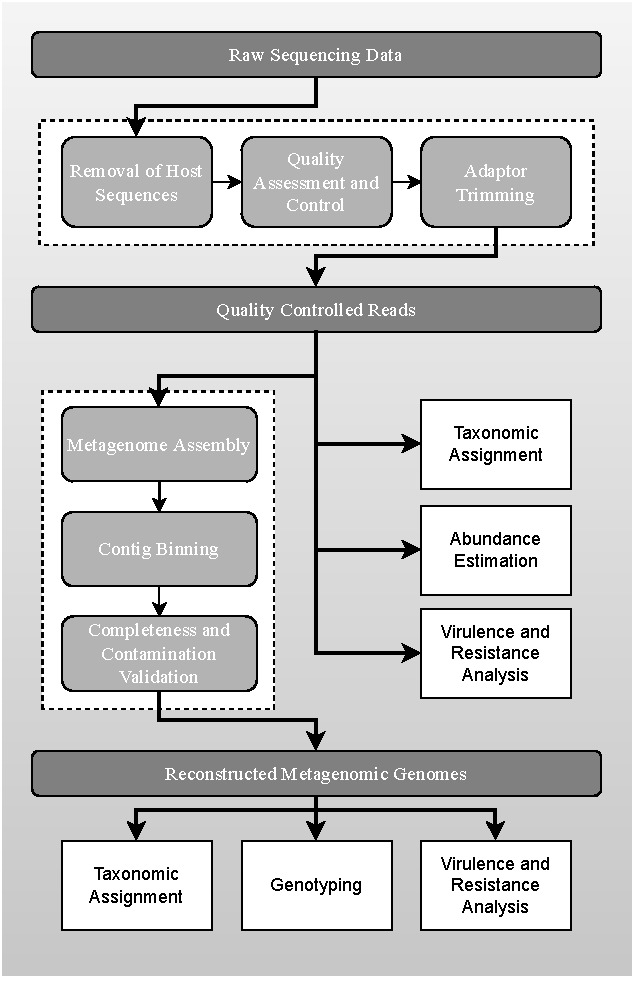
\includegraphics[angle=0,width=\textwidth]{figures/introduction/Figure9.pdf}
    \caption[SNP-based methods]{SNP-based methods map the sequencing reads or genome assemblies from bacterial strains against a reference genome to identify \ac{SNPs}. The top sequence in the image represents a region of the reference genome and the bottom lines represent the same region for a group of strains. The positions that differ from the reference genome are colored in red.}
    \label{fig:introduction_figure9}
\end{figure*}

\subsubsection{\textit{k}-mer-based methods}

Although the concept of \textit{k}-mer has existed for several decades, even if under different designations (e.g., N-gram, k-tuple, w-mers), its wide application to increase the efficiency and accuracy of bioinformatics methods is relatively recent. \textit{k}-mer-based approaches break sequences into smaller subsequences of length \textit{k}. This seemingly simple approach of \textit{break it to understand it} has enormous potential, allowing for much more time-efficient sequence comparisons than alignment-based approaches. However, storing large sets of \textit{k}-mers in memory can lead to high memory usage. Thus, it is important to optimize parameters such as the \textit{k}-mer size and sampling method, also termed sketching (i.e., which \textit{k}-mers to select from all possible \textit{k}-mers generated from a sequence). With respect to \textit{k}-mer size, it is important to optimize it for the desired application by balancing the trade-off between greater specificity achieved with longer \textit{k}-mers and greater sensitivity with shorter \textit{k}-mers. Optimizing \textit{k}-mer selection is more complex and has been the subject of extensive research \cite{roberts_reducing_2004, sahlin_effective_2021, ndiaye_when_2024, karami_designing_2024, kille_minmers_2023, shaw_theory_2022}.

\begin{figure*}[h!]
    \centering
    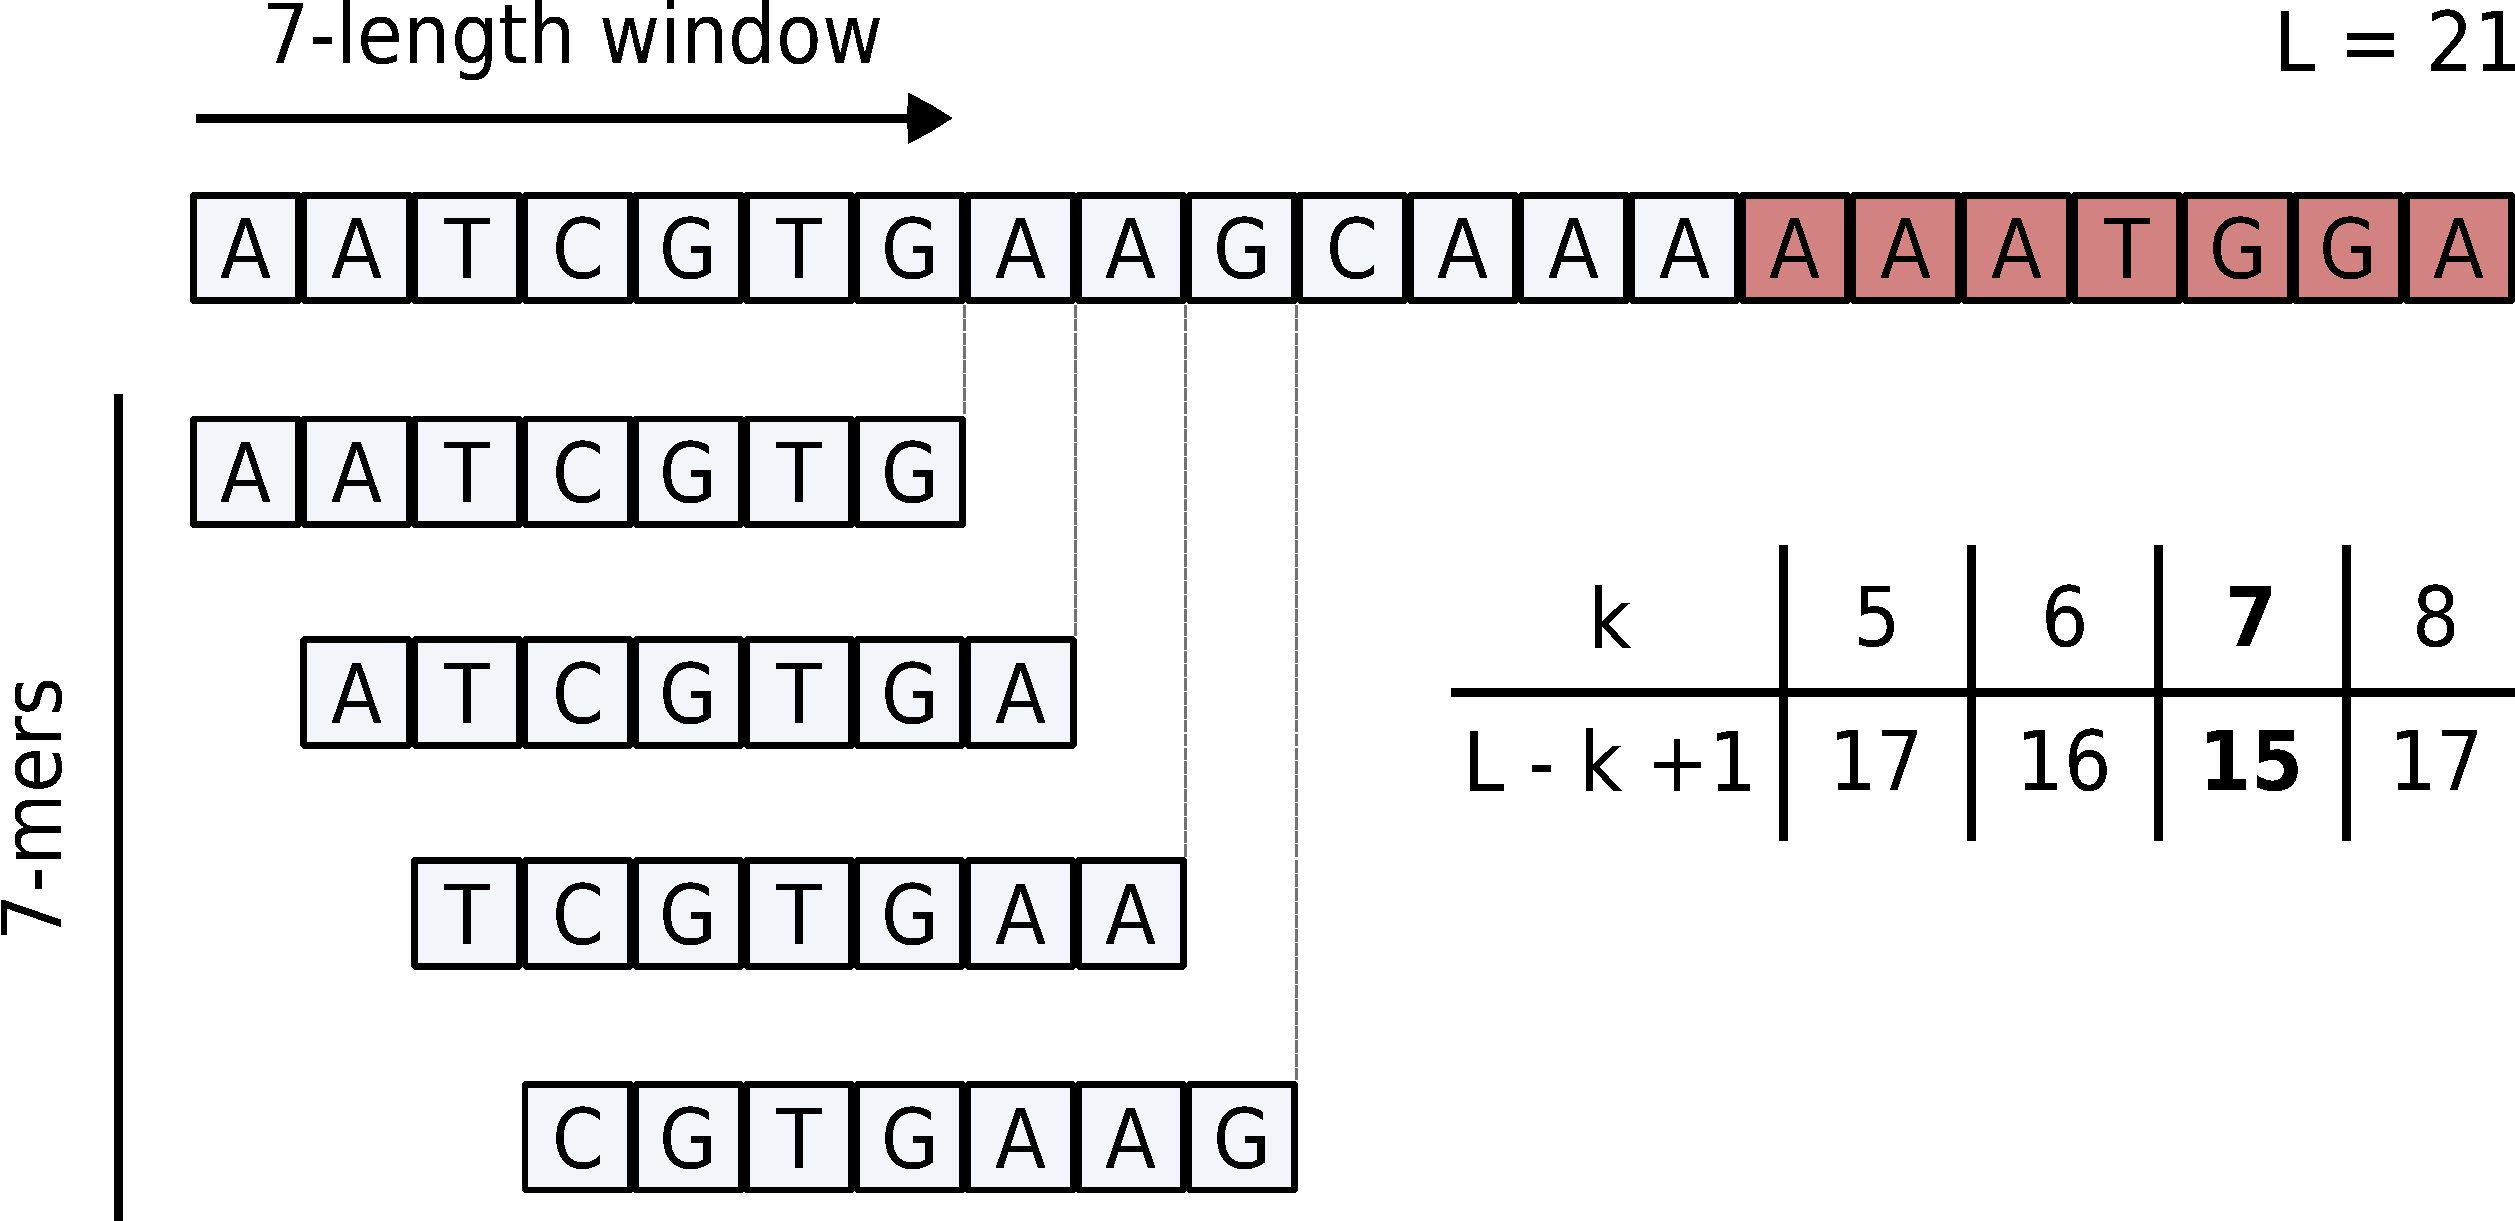
\includegraphics[angle=0,width=\textwidth]{figures/introduction/Figure10.pdf}
    \caption[Determining \textit{k}-mers]{Determining \textit{k}-mers. After defining the value of \textit{k}, the first \textit{k}-mer is determined by selecting the segment with the first \textit{k} bases in the sequence. The next \textit{k}-mer is determined by sliding one position to the right to select a new \textit{k}-mer that differs from the first one by a single position. This process is repeated until all consecutive \textit{k}-mers are determined. The figure represents the determination of 7-mers from a sequence with 21 nucleotides (L). The first four 7-mers are shown below the sequence. The last 7-mer is highlighted in red. The table shows the total number of \textit{k}-mers that can be determined from the sequence by varying the value of \textit{k} from 5 to 8. The column corresponding to the total number of 7-mers is in bold.}
    \label{fig:introduction_figure10}
\end{figure*}

Ideally, it is desired to select the smallest set of \textit{k}-mers that minimizes memory usage without sacrificing accuracy. However, depending on the application, it may be necessary to satisfy other requirements that complicate the determination of the optimal sampling method. For example, a sampling method that selects \textit{k}-mers randomly may be preferred for unbiased sequence comparisons, while optimizing the interval between consecutively selected \textit{k}-mers may offer better performance when sequence variability is higher. Theoretical and empirical evaluations of the performance of each sampling method are important to determine optimal parameters and limitations. Minimizers and spaced seeds are two sampling methods that have been widely applied due to their simplicity and effectiveness in a wide range of applications, such as genome assembly and taxonomic classification. \textit{k}-mers are a centerpiece of most genome assemblers, with the construction of \textit{de Brujin} graphs, representing the overlap between \textit{k}-mers determined from sequencing reads, being the fundamental strategy used by many genome assemblers to solve the problem of genome assembly for both short- and long-read data \cite{medvedev_what_2021}. For taxonomic classification, sequence data are often decomposed into \textit{k}-mers and compared against \textit{k}-mer indexes constructed from taxonomically annotated reference sequences. This strategy allows for ultra-fast taxonomic classification. Kraken was one of the first highly successful \textit{k}-mer based tools for taxonomic classification \cite{wood_kraken_2014}. Its first version enabled fast taxonomic classification based on a minimizer index, and the second version optimized the database structure to reduce memory requirements and added spaced seeds for greater accuracy \cite{wood_improved_2019}. In theory, \textit{k}-mer-based methods offer several advantages over \ac{wg/cgMLST} and \ac{SNP}-based methods. Firstly, there is no need to define a reference database, such as a schema, or select a reference genome to compare strains against. This overcomes the reference bias limitation of \ac{SNP}-based approaches and eliminates the need to store and manage a schema with a specific allelic nomenclature. However, to achieve consistent results, especially when trying to establish a cluster nomenclature, it is still recommended to create a database structure to compare and classify strains. Otherwise, the results obtained for different datasets may not be comparable. Secondly, and contrary to \ac{wg/cgMLST}, \textit{k}-mer-based methods can include non-coding regions to estimate strain similarity. Lastly, if adequately parameterized, \textit{k}-mer-based methods can be faster and more efficient than \ac{wg/cgMLST} or \ac{SNP}-based methods. A good example of an efficient and versatile \textit{k}-mer-based method applicable to closely related samples and outbreak investigation is SKA2 \cite{derelle_seamless_2024}. SKA2 uses split \textit{k}-mer analysis for reference-free and reference-based mapping to genotype bacterial strains using sequencing reads or genome assemblies. Another \textit{k}-mer based tool, PopPUNK \cite{lees_fast_2019}, uses \textit{k}-mers to calculate core and accessory distances, which in turn are used by machine learning algorithms to cluster bacterial strains. This approach has proved useful for population analysis, and the ability to update existing clusters with new strains without having to recalculate all pairwise distances is especially useful for surveillance.

\section{Aims of the Thesis}

The advances in \ac{DNA} sequencing technologies have allowed research and public health institutions to gradually switch from classical and more laborious microbiological workflows to \ac{WGS}-based methods for the characterization of bacterial pathogens. With modern sequencing technologies, it is possible to streamline the genome sequencing of dozens of bacterial strains. The widespread adoption of \ac{WGS} and the increased availability of bacterial genomes in public databases enabled researchers to develop and apply more advanced bioinformatics methods to gain greater insight into the structure, diversity and dynamics of bacterial genomes. \ac{GbG}, \ac{SNP}-based and \textit{k}-mer-based methods allow for a more detailed characterization of bacterial pathogens and are currently widely applied for surveillance, outbreak investigation, and to study the diversity of bacterial species. \ac{GbG} methods in particular, such as \ac{wg/cgMLST}, have been adopted more frequently for surveillance and outbreak investigation, perhaps in part because they constitute an expansion of the classical seven-gene \ac{MLST}, making it conceptually and technically easier to implement and transition to. The wide adoption of \ac{wg/cgMLST} makes it relevant to explore ways in which it can be further improved. The main objective of this work is to explore concepts and implement solutions that improve the efficiency, accuracy, and interoperability of \ac{wg/cgMLST}. The main goals are the following.

- Optimize the processes of schema creation and allele calling in \ac{wg/cgMLST}, as well as implement solutions for comprehensive analysis of the schema and results data;

- Implement a Nomenclature Server to store and manage \ac{wg/cgMLST} schemas that enables local and private analyzes based on a common allelic nomenclature;

- Identify and propose solutions for common problems found in \ac{wg/cgMLST} schemas, either derived from low-quality data or from limitations of current methodologies used in \ac{wg/cgMLST}.

The first goal will be achieved mainly through the optimization of the chewBBACA software for \ac{wg/cgMLST} \cite{silva_chewbbaca_2018}. The second goal will focus on creating a Web service that provides easy access to \ac{wg/cgMLST} schemas and minimizes scalability and data privacy concerns compared to other well-known \ac{wg/cgMLST} platforms that centralize data analysis and require users to share their data. The last goal will help create strategies to identify and correct spurious loci added to \ac{wg/cgMLST} schemas, improve the integration of accessory loci into \ac{wgMLST} schemas, and provide valuable information to guide the development of chewBBACA.


%-----------------------------------------------------------------
% Paper 1 - chewBBACA 3
%------------------------------------------------------------------
\newpage
\thispagestyle{empty}
\chapter{chewBBACA 3: lowering the barrier for scalable and detailed whole- and core-genome multilocus sequence typing\label{ch:paper1}}
\thispagestyle{empty}
\cleardoublepage
\mbox{}\\
\vspace{8cm}

This chapter is a reproduction of the following article:

R. Mamede, P. Vila-Cerqueira, J. A. Carriço, M. Ramirez. chewBBACA 3: lowering the barrier for scalable and detailed whole- and core-genome multilocus sequence typing. (2025)


% N. Couto, L. Schuele, E.C. Raangs, M. P. Machado, C. I. Mendes, T. F. Jesus, M. Chlebowicz,  S. Rosema, M. Ramirez, J. A. Carriço, I. B. Autenrieth, A. W. Friedrich, S. Peter and J. W. Rossen. Critical steps in clinical shotgun metagenomics for the concomitant detection and typing of microbial pathogens. Sci Rep 8, 13767 (2018). DOI: \url{https://doi.org/10.1038/s41598-018-31873-w}

The supplementary information referred to throughout the text can be consulted in this chapter before the References section. 

As mentioned in Chapter \ref{ch:introduction}, section \ref{sssec:_intro_shotgun_metagenomics}, \ac{SMg} approaches have been a growing interest to deliver clinically relevant results without \textit{a priori} knowledge of what to expect from a particular clinical sample or patient. 
The capacity to detect all potential pathogens in a sample has great potential utility in the diagnosis of infectious disease. 
However, it is unclear how the variety of available methods impacts the end results.

In this publication, \ac{SMg} was applied to nine body fluid samples and one tissue sample from patients at the University Medical Center Groningen with varying degrees of contamination: one sample from peritoneal fluid, five from pus, two from synovial fluid of knees with a prosthesis, one from sputum and one from a bone biopsy. The results of microbial identification through whole genome sequencing (\ac{WGS}) and \ac{SMg} were compared to standard culture-based microbiological methods. 
In order to evaluate and compare the accuracy and reliability of the bioinformatics analyses in providing the closest results to culture and \ac{WGS} of any cultured isolates, three different bioinformatic pipelines (two commercially and one freely available) were used. Most pathogens identified by culture were also identified through metagenomics, but substantial differences were noted between the taxonomic classification tools. 

My contribution to this publication included the bioinformatics analysis of all the samples using a Unix-based approach. I performed quality assessment and quality control of the \ac{WGS} and \ac{SMg} data, the removal of host sequencing from the samples, and the taxonomic identification of the remaining reads in each sample through 3 different methods: MetaPhlan2, Kraken and MIDAS. Gene detection directly from the reads for bacterial typing was also performed using metaMLST, ReMatCh, Bowtie2 and Samtools. Finally, the reads were assembled using the SPAdes genome assembler, with and without metagenomic mode according to the sample being processed. 

\cleardoublepage 

\begin{center}
\large
\textbf{chewBBACA 3: lowering the barrier for scalable and detailed whole- and core-genome multilocus sequence typing}
\end{center}

Rafael Mamede$^{1,2}$, 
Pedro Vila-Cerqueira$^{1}$,
João André Carriço$^{1}$,
Mário Ramirez$^{1}$

$^1$ Instituto de Microbiologia, Instituto de Medicina Molecular, Faculdade de Medicina, Universidade de Lisboa, Portugal;

$^2$ Gulbenkian Institute for Molecular Medicine.

\section{Abstract} \label{sec:ch2_abstract}

\subsection{Background} \label{ssec:ch2_abstract}

The wide adoption of whole genome sequencing has enabled the implementation of genomics-based systems, which provide unparalleled resolution for the surveillance and outbreak investigation of bacterial pathogens. To fully exploit the wealth and complexity of genomics data, bioinformatics methods need to be highly scalable, provide accurate and extensive data for potential downstream analyses, as well as analytic capabilities. Here, we present chewBBACA 3, a suite of modules for scalable and comprehensive bacterial whole- and core-genome multilocus sequence typing (wg/cgMLST) with built-in features to create new schemas, evaluate loci diversity and strain similarity.

\subsection{Results} \label{ssec:ch2_abstract}

chewBBACA 3 enables faster and more accurate schema creation and allele calling by complementing an alignment-based approach with alignment-free methods, including hash-based comparisons and minimizer-based clustering. Schema creation is up to 55-fold faster and identifies up to 10\% more loci than its predecessor, chewBBACA 2. Furthermore, chewBBACA 3 can quickly adapt or import schemas available on external wg/cgMLST platforms or Chewie-NS, promoting interoperability. The efficiency of allele calling allows processing larger genome collections, from thousands to tens of thousands of genomes, at the whole- and core-genome levels without requiring high computational resources and being up to 52-fold faster than similar tools. chewBBACA 3’s enhanced sensitivity allows it to identify and classify more schema loci and coding sequences than the compared methods, resulting in higher resolution for strain comparison. Moreover, the allelic profiles, classification statistics and associated sequence data produced by chewBBACA 3 can be the basis for detailed analyses that provide added value in surveillance and outbreak investigation settings. New modules leverage the potential of the schema and allele call results data to create interactive reports that enable an intuitive and in-depth analysis of allele diversity in loci of interest and allow assessing strain similarity based on loci presence, allelic distances and phylogenetic analysis.

\subsection{Conclusions} \label{ssec:ch2_abstract}

chewBBACA 3 provides functionalities for complete wg/cgMLST analysis at scale, lowering the barrier for the use of wg/cgMLST and offering extensive results and analytic capabilities for streamlined, comprehensive, and local analyses. chewBBACA 3 is freely available at \url{https://github.com/B-UMMI/chewBBACA}.

\section{Background} \label{sec:ch2_background}

The burden of bacterial infections constitutes a major challenge to public health systems worldwide \citep{ikuta_global_2022, noauthor_who_2024}. The advances in sequencing technologies have enabled public health institutions to support and gradually transition to whole genome sequencing (WGS), increasing surveillance capacity and the effectiveness of outbreak investigations. WGS offers high-resolution discrimination of closely related bacterial strains and enables the identification of pathogens’ relevant features in a timely and accurate manner, aiding in reaching an informed decision for effective disease prevention and control \citep{authority_efsa_efsa_2024, struelens_real-time_2024, european_centre_for_disease_prevention_and_control_ecdc_2019, authority_efsa_guidelines_2022}. The widespread use of WGS, as well as the adherence to FAIR principles, encouraged the development of efficient bioinformatics methods for in silico multilocus sequence typing (MLST), serotyping, and the identification of antimicrobial resistance and virulence determinants. It also allowed transitioning to methods with enhanced resolution that leverage the full genomic content to identify relevant features and provide a more accurate measure of strain similarity \citep{uelze_typing_2020}.

These methods are diverse but generally adopt one of three fundamental approaches: i) determining Single-Nucleotide Variants (SNVs) relative to a reference genome, ii) measuring sequence similarity based on short subsequences of length k, known as k-mers, and iii) comparing the strains' gene content, referred to as gene-by-gene methods (GbG) \citep{uelze_typing_2020}.

SNV approaches detect differences at the single nucleotide level by mapping sequencing reads against a closely related reference strain. The precision level of this approach enables the identification of point mutations or more complex variants that can be determinants of phenotypic characteristics of interest, such as increased virulence and antimicrobial resistance. The choice of the reference genome is crucial as the quality and relatedness of the reference genome to the strains of interest can greatly influence the number of shared positions compared and, therefore, the extent of the variability detected \citep{bush_genomic_2020, valiente-mullor_one_2021}. k-mer-based tools split genomic sequences into k-mers and compare the resulting k-mer sets to estimate strain similarity or identify regions of interest. These approaches can estimate similarity without needing a reference genome and are potentially faster and more computationally efficient than SNV or GbG approaches. The efficiency of these approaches depends on the sampling method used to select k-mers, which should be fine-tuned to achieve a good balance between efficiency and accuracy for the desired application \citep{ndiaye_when_2024, belbasi_minimizer_2022}. With the wide adoption of WGS, GbG approaches have transitioned from classical MLST to whole-genome and core-genome MLST (wg/cgMLST). wg/cgMLST enables the creation of schemas encompassing the variability of hundreds to thousands of loci for a species of interest to accurately determine the loci and alleles present in strains of interest. Creating and maintaining wg/cgMLST schemas to capture a species' diversity is crucial for the accuracy of GbG methods and can be a laborious process. As with SNV approaches, knowing the alleles present at a given locus can be linked to phenotypic properties such as virulence or antimicrobial resistance.

It has been shown that applying any of these approaches can generate results suitable for accurate strain similarity estimation and phylogenetic analyses in surveillance and outbreak scenarios \citep{uelze_typing_2020, bush_genomic_2020, valiente-mullor_one_2021, ndiaye_when_2024, belbasi_minimizer_2022, king_comparison_2024}. Nevertheless, wg/cgMLST has been more frequently integrated into surveillance and outbreak detection systems, partly due to constituting an expansion of classical MLST, which conceptually and technically allows for a more straightforward implementation, specially in constantly growing datasets such as the ones used in long-term epidemiological surveillance. The capacity to update wg/cgMLST schemas with new alleles increases the diversity captured by and, consequently, the resolution of wg/cgMLST analyses. Moreover, wg/cgMLST allows establishing allelic nomenclatures for standardised comparisons. Existing solutions for wg/cgMLST analysis can vary greatly in the degree of data centralisation, analytical capabilities, and license type \citep{jolley_bigsdb_2010, zhou_enterobase_2020, mamede_chewie_2021}. To continue to promote the adoption of wg/cgMLST, improvements should focus on interoperability to facilitate comparison of results, scalability to meet growing data processing demands, and easily performed comprehensive local analyses to offer powerful analytic capabilities to end users while complying with strict data privacy laws.

To provide a solution for scalable, detailed, and local wg/cgMLST, we developed chewBBACA 3, which vastly improves and extends the functionalities of chewBBACA 2 \citep{mamede_chewie_2021, silva_chewbbaca_2018}, a widely used tool for wg/cgMLST which has been integrated into public health workflows such as EFSA's One Health WGS system, used for rapid detection of multi-country foodborne outbreaks in collaboration with the European Centre for Disease Prevention and Control (ECDC) \citep{authority_efsa_guidelines_2022}.

\section{Implementation} \label{sec:implementation}

\subsection{Overview} \label{ssec:overview}

chewBBACA 3 is a complete reimplementation of its predecessor, chewBBACA 2 \citep{mamede_chewie_2021}, which was already an upgraded version of chewBBACA’s first published version \citep{silva_chewbbaca_2018}. chewBBACA 3 provides a modular approach for complete wg/cgMLST analysis allowing more efficient and accurate schema creation and allele calling and offering interactive reports for comprehensive schema and results analyses \ref{fig:chap2_figure1A}. chewBBACA 3 allows to set up schemas for wg/cgMLST through the use of larger collections of genome assemblies or coding DNA sequences (CDSs) in FASTA format or by adapting existing schemas from external platforms \citep{jolley_bigsdb_2010, zhou_enterobase_2020, noauthor_cgmlstorg_nodate}. Additionally, the integration with Chewie-NS, which was previously described together with chewBBACA 2 \citep{mamede_chewie_2021}, allows easily importing ready-to-use schemas to obtain comparable interlaboratory results based on a common allelic nomenclature. To determine the allelic profiles of strains of interest, chewBBACA 3 identifies and clusters the distinct CDSs predicted from the strains' genomes, significantly reducing the number of comparisons against the schema loci in contrast to the sequential strain processing used by chewBBACA 2. This translates into faster and more efficient allele calling and facilitates data aggregation to create output files with more detailed results. Allele calling identifies and adds new alleles to schemas, ensuring that they are gradually updated to produce accurate and comparable results over time. Similarly to chewBBACA 2, new alleles are inferred based on the BLAST Score Ratio (BSR) \citep{rasko_visualization_2005} computed from BLASTp alignments \citep{camacho_blast_2009}, complying with minimum sequence length and allele size variation thresholds \citep{silva_chewbbaca_2018}. Adjustments to these parameters allow chewBBACA 3 to classify more CDSs and capture loci diversity more accurately. chewBBACA 3 increases the granularity of the results by expanding the set of special classifications assigned when the presence of a locus cannot be inferred confidently, such as when a CDS matching a schema locus is outside the user-specified locus size variation interval or if multiple CDSs from a genome match the same schema locus \ref{fig:chap2_figureS1, fig:chap2_figureS2, fig:chap2_figureS3, fig:chap2_figureS4}(Figures S1-S4, Additional File 1). These special classifications aid in identifying spurious alleles resulting from low-quality data, pseudogenes, and paralogous loci. The set of core loci can be determined based on the allele calling results for any locus presence threshold, and the resulting list of core loci can be used to perform allele calling at the core genome level. Schema loci can be annotated by searching for matches through UniProt’s SPARQL endpoint, which was already an option in chewBBACA 2, and now also by aligning a schema’s alleles against UniProt’s reference proteomes to retrieve annotations based on higher-quality entries \citep{the_uniprot_consortium_uniprot_2025}. New schema and results evaluation modules leverage the power of the React JavaScript library \citep{noauthor_react_nodate} to build interactive reports that enable local and comprehensive analyses of the diversity of loci contained in schemas and aid in identifying closely related strains for more effective surveillance and outbreak assessment.

\subsection{Core modules} \label{ssec:core_modules}

While all the modules in chewBBACA 2 were reimplemented to increase the scalability and comprehensiveness of the results generated by chewBBACA 3, module development concentrated primarily on the CreateSchema and AlleleCall modules (Figures S5 and S6, Additional File 1), which handle schema creation and allele calling, respectively. Gene prediction was optimised in both modules using Pyrodigal \citep{larralde_pyrodigal_2022, hyatt_prodigal_2010}, a Python module that provides bindings to Prodigal for seamless integration and offers several advantages, such as faster gene prediction and greater control over gene prediction parameters and results. Additionally, a novel feature was added allowing both modules to accept FASTA files with CDSs, enabling users to leverage the vast CDS data available in public databases or provide CDSs predicted by other gene prediction tools if preferred by the user, such as GeneMarkS-2 or Balrog \citep{lomsadze_modeling_2018, sommer_balrog_2021}. Following the gene prediction step, CDS deduplication is performed at both DNA and protein levels to identify the set of distinct CDSs. The distinct translated CDSs are clustered based on the proportion of shared minimizers ($\geq0.2$) with representative alleles \citep{schleimer_winnowing_nodate, roberts_reducing_2004, marcais_improving_2017} (Figure 1B:1-3). The minimizer parameters (k=5, w=5, lexicographic order) were chosen to select sets of k-mers that would cover most sequence positions at least once while also keeping memory usage low \citep{zheng_improved_2020}. The low clustering threshold groups similar sequences into the same clusters, reducing the number of comparisons in subsequent steps. For schema creation, the CDSs sharing a high proportion of minimizers ($\geq0.9$) with the cluster representative or larger CDSs are considered alleles of the same locus and are excluded (Figure 1B:4). The clustering results are complemented by intracluster and intercluster alignment with BLASTp to exclude CDSs based on the BSR threshold and select the final set of CDSs (Figure 1B:5). This defines the schema by creating a schema seed with one representative allele for each locus. This schema seed will be used by the AlleleCall module, which may add further representative alleles to capture the allelic diversity at each locus. The AlleleCall module uses the same functions as the schema creation process for sequence deduplication and CDS clustering. Another novel feature implemented is that each distinct CDS is hashed, mapped to the compressed list of genomes that contain it (Figure S7, Additional File 1) and compared against the hashed schema alleles. This allows keeping the information about the CDSs identified in all strains in memory, enabling fast exact matching and classification of all genomes containing a CDS based on a single match. Clustering and intracluster alignment with BLASTp allow comparison of the remaining unclassified CDSs against the schema's representative alleles to find and classify inexact matches (Figure 1B:1-4). A final step aligns the schema's representative alleles against the remaining unclassified CDSs to find more divergent alleles and select new representative alleles (Figure 1B:5). The matches found throughout the process are evaluated at the end of the process to assign the final classifications, create the allelic profiles, and update the schema with novel alleles. Both core modules create several output files with detailed schema and results data that support the analyses performed by other modules and can serve as the basis for custom analyses that seek to answer relevant questions at the strain or population-wide level.
A more detailed description of the implementation and functionalities included in each module is available in the supplementary material (Additional File 1) and in chewBBACA’s online documentation \citep{noauthor_chewbbaca_nodate}.

\begin{figure*}[h!]
    \centering
    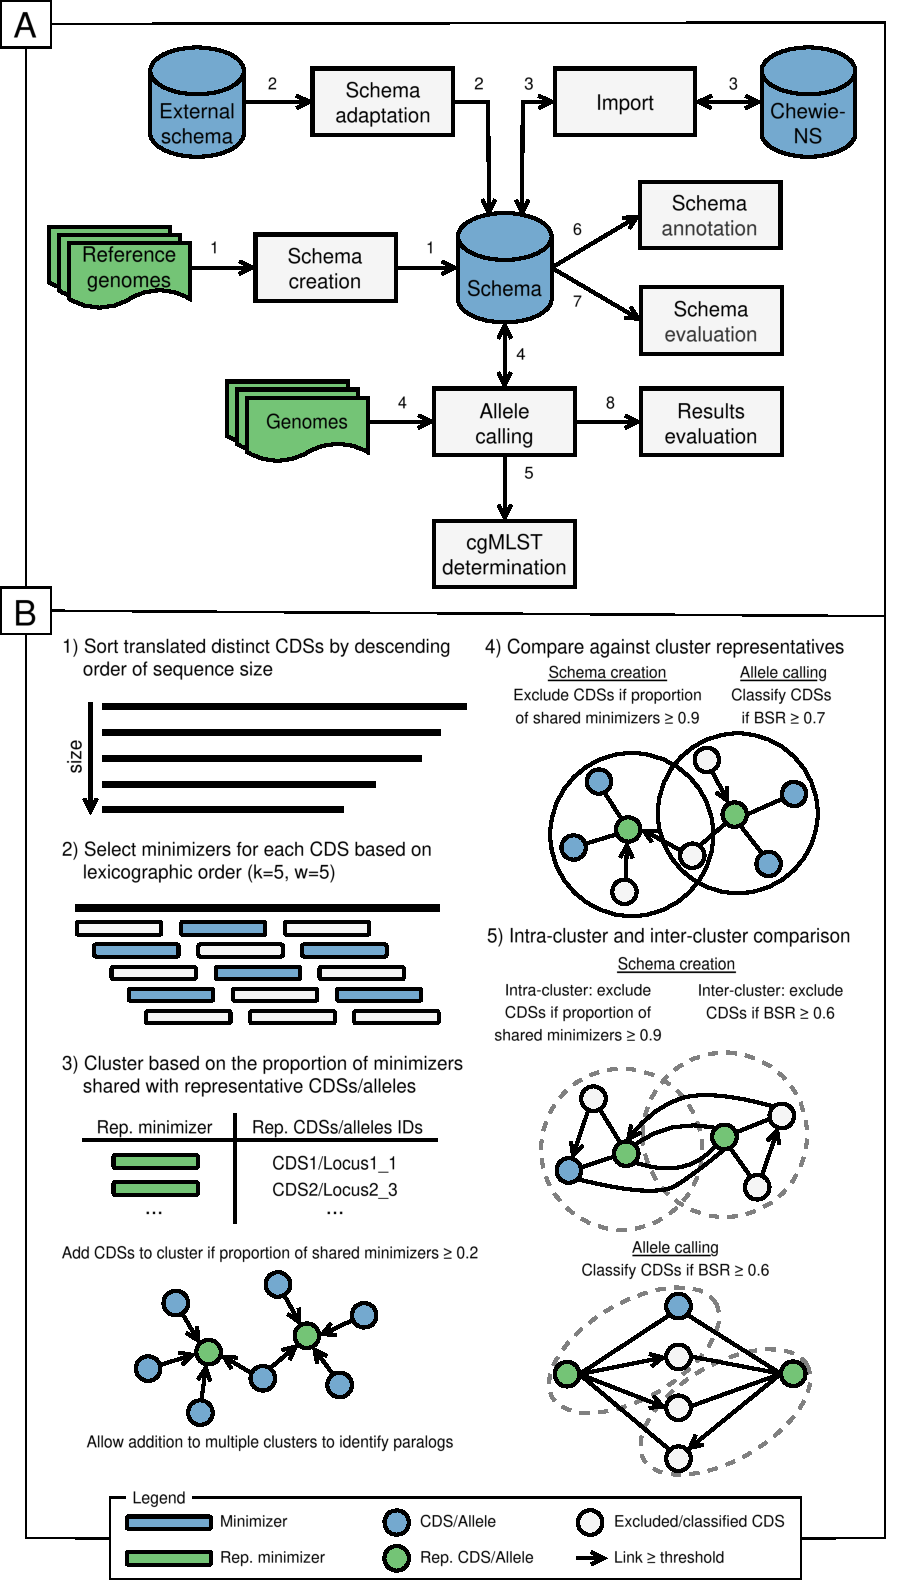
\includegraphics[angle=0,height=0.92\textheight]{figures/chapter 2/Figure1.pdf}
    \label{fig:chap2_figure1}
\end{figure*}
\vspace*{-6mm}
\begin{center}
    \emph{(Caption on next page.)}
\end{center}
\begin{figure*}[h!]
    \caption{Overview of chewBBACA 3’s processes and minimizer-based clustering used by the \textit{CreateSchema} and \textit{AlleleCall} modules. (A) chewBBACA 3 includes modules for schema setup (steps labeled with 1, 2 and 3), allele calling (steps labeled with 4), core genome determination (steps labeled with 5), schema annotation (steps labeled with 6), schema evaluation (steps labeled with 7), and results evaluation (steps labeled with 8). Blue cylinder icons represent schemas, with the central cylinder icon representing a schema created or adapted for usage with chewBBACA 3. Green document icons represent input FASTA files. Grey rectangle icons represent analysis processes available in chewBBACA 3. (B) Minimizer-based clustering and classification steps implemented in the \textit{CreateSchema} and \textit{AlleleCall} modules. (Step 1) The distinct translated CDSs not classified through exact matching at the DNA and protein levels are sorted based on decreasing size. (Step 2) Minimizers are selected from the set of 5-mers for each CDS based on lexicographic order and a window size of 5. (Step 3) The set of minimizers selected for each CDS is compared against the minimizers of CDSs selected as cluster representatives (\textit{CreateSchema}) or the schema loci representative alleles (\textit{AlleleCall}) to cluster CDSs based on a proportion of shared minimizers $\geq0.2$. (Step 4) The CDSs that share a proportion of minimizers $\geq0.9$ (\textit{CreateSchema}) or a BSR $\geq0.7$ (AlleleCall) with the cluster representative are excluded from the analysis (\textit{CreateSchema}) or classified (\textit{AlleleCall}). (Step 5) Non-representative CDSs from the same cluster are compared to exclude smaller CDSs that share a proportion of minimizers $\geq0.9$ with larger CDSs (CreateSchema). Representative CDSs or alleles are aligned against all CDSs to exclude (\textit{CreateSchema}) or classify (\textit{AlleleCall}) CDSs based on a default BSR value of 0.6.}
\end{figure*}


% (Table \ref{tab:ch2_table_1}).
% \ref{fig:chap2_figure1A}
% \begin{landscape}
% \begin{table}[]
\caption{Characteristics of the samples and mapping of trimmed reads against a human genome hg19 (\%) using CLC Genomics Workbench v10.0.1.}
\label{tab:ch2_table_1}
\resizebox{\linewidth}{!}{%
\small
\begin{tabular}{@{}llllll@{}}
\toprule
\textbf{Sample} & \textbf{Sample type} & \textbf{DNA extraction method} & \textbf{Total number of reads} & \textbf{Mapped reads against hg19} & \textbf{Unmapped reads} \\ \midrule
Sample 1         & Peritoneal fluid & Ultra-Deep Microbiome Prep (Molzym) & 5892978 & 5,249,063 (89.2\%) & 632,951 (10.8\%)   \\
Sample 2         & Pus (abscess)    & Ultra-Deep Microbiome Prep (Molzym) & 9603346 & 7,828.746 (81.6\%) & 1,770,558 (18.4\%) \\
Sample 3         & Synovial fluid   & Ultra-Deep Microbiome Prep (Molzym) & 8615810 & 8,254,594 (95.9\%) & 355,200 (4.1\%)    \\
Sample 4         & Synovial fluid   & Ultra-Deep Microbiome Prep (Molzym) & 6078166 & 6,015,945 (99.0\%) & 61,099 (1.0\%)     \\
Sample 5         & Pus (abscess)    & Ultra-Deep Microbiome Prep (Molzym) & 8368930 & 309,588 (3.7\%)    & 8,052,272 (96.3\%) \\
Sample 6         & Pus (empyema)    & QIAamp DNA Microbiome Kit (Qiagen)  & 2912802 & 2,877,066 (98.8\%) & 34,506 (1.1\%)     \\
Sample 7         & Pus (empyema)    & QIAamp DNA Microbiome Kit (Qiagen)  & 1486700 & 922,932 (62.2\%)   & 561,772 (37.8\%)   \\
Sample 8         & Bone biopsy      & Micro-DXTM (Molzym)                 & 6534866 & 229,149 (3.5\%)    & 6,303,803 (96.5\%) \\
Sample 9         & Pus (abscess)    & Micro-DXTM (Molzym)                 & 6173132 & 6,081,612 (98.5\%) & 89,922 (1.5\%)     \\
Sample 10        & Sputum           & Micro-DXTM (Molzym)                 & 7596836 & 7,337,832 (96.7\%) & 235,520 (3.3\%)    \\
Negative control & Water            & QIAamp DNA Microbiome Kit (Qiagen)  & 1730738 & 1,706,861 (98.9\%) & 19,805 (1.2\%)     \\ \bottomrule
\end{tabular}%
}
\end{table}
% \end{landscape}

%0.2 ng/$\mu$l and 1 ng
%\ref{tab:ch2_table_1})

% Reference scronyms
%\ac{WGS}
%All the parameters used in each approach are available in Supplementary Table 1 (see \ref{ch2_supmaterial}).

\section{Results and discussion} \label{sec:results_and_discussion}

\subsection{Fast wg/cgMLST schema creation or retrieval from multiple sources} \label{ssec:results_discussion_ssec1}

chewBBACA 3 offers three options for setting up a schema for wg/cgMLST analysis.

The first option is creating a new schema by selecting loci from a set of complete or draft genome assemblies with the CreateSchema module to create a schema seed (Figure S5, Additional File 1). To evaluate the performance of the CreateSchema module, we created schema seeds with chewBBACA 3 and chewBBACA 2 based on the complete genome assemblies available on the NCBI RefSeq database \citep{sayers_database_2022} for three bacterial species: Streptococcus pyogenes (n=260), Listeria monocytogenes (n=309), and Salmonella enterica (n=1,326). Schema seed creation was 25- to 55-fold faster with chewBBACA 3 than with chewBBACA 2, with similar memory usage (Table S1, Additional File 2). A comparison of the schema seeds generated with both versions revealed that the schema seeds created by chewBBACA 3 contained 98\% of the loci identified by chewBBACA 2 (Table S2, Additional File 2). Moreover, chewBBACA 3 identified 6\% to 10\% more loci than chewBBACA 2, primarily due to a more accurate identification of smaller loci. Ideally, target loci should be defined based on a set of high-quality genome assemblies to avoid the inclusion of spurious loci in the schema seed. Nonetheless, schema seed creation with chewBBACA 3 will remain efficient even when using larger genome collections, possibly including draft genomes, to adequately capture a species diversity.

A second option is to adapt schemas from external platforms with the PrepExternalSchema module (Figure S8, Additional File 1). This module filters out incomplete alleles (i.e. alleles that contain ambiguous bases or not corresponding to valid CDSs, such as having no start/stop codon) and selects representative alleles based on a BSR threshold to create a schema structure compatible with chewBBACA. Schema adaptation promotes the usage of schemas previously made available and adopted by the community, contributing to the integration and interoperability with other platforms. chewBBACA 3 is over three orders of magnitude faster than chewBBACA 2 when adapting the cgMLST schemas for S. pyogenes, L. monocytogenes, and S. enterica available on the cgMLST.org server \citep{noauthor_cgmlstorg_nodate}, adapting any of the schemas in under five minutes (Table S3, Additional File 2). Furthermore, contrarily to chewBBACA 2, chewBBACA 3 now ensures that the selected representative alleles fully capture the diversity of each locus based on the specified BSR threshold (Table S4, Additional File 2). chewBBACA 3 also provides options to filter out alleles based on user-defined sequence size and size variation thresholds and outputs detailed information about the changes made while adapting a schema to inform the user of the changes introduced to the existing schema.

Lastly, the third option is the DownloadSchema module (Figure S9, Additional File 1), one of the modules (Figures S9-S11, Additional File 1) developed to integrate with Chewie-NS \citep{mamede_chewie_2021} [15], allowing users to import ready-to-use schemas from Chewie-NS instances. This option offers the advantage of enabling local and private analysis based on a common allelic nomenclature to facilitate the comparison of results. Schemas downloaded from Chewie-NS can be kept up-to-date by synchronizing with the remote versions to receive the latest allele data submitted by other users and, if desired, contribute novel alleles identified locally.

\subsection{Scalable and efficient allele calling} \label{ssec:results_discussion_ssec2}

We performed allele calling with the schema seeds created with chewBBACA 3 in the previous section and the complete genomes for each species to add new alleles to the schemas and determine the set of core loci with the ExtractCgMLST module (Figure S12, Additional File 1). The lists of core loci (present in 100\% of the genomes) were used to measure performance at the cgMLST level for datasets including between 1 and 16,384 draft genome assemblies and compared against the results obtained with chewBBACA 2 and pyMLST \citep{biguenet_introduction_2023} for equivalent schemas and databases (Table S5, Additional File 2). chewBBACA 3 processed all datasets faster than chewBBACA 2 and pyMLST. On average, chewBBACA 3 was 1.9- to 20.3-fold and 1.3- to 51.9-fold faster than chewBBACA 2 and pyMLST, respectively (Figure 2A and Table S6, Additional File 2). The difference increased with dataset size, largely due to the increased redundancy (same sequence found in different genomes) of the set of CDSs extracted from the genomes (Table S7, Additional File 2). For example, only 1.5\% to 2.8\% of the total CDSs identified in the complete datasets (n=16,384) were distinct. By identifying the set of distinct CDSs before trying to match them against the schema loci, chewBBACA 3 avoids the repeated evaluation of identical CDSs identified in multiple genomes.

\begin{figure*}[h!]
    \centering
    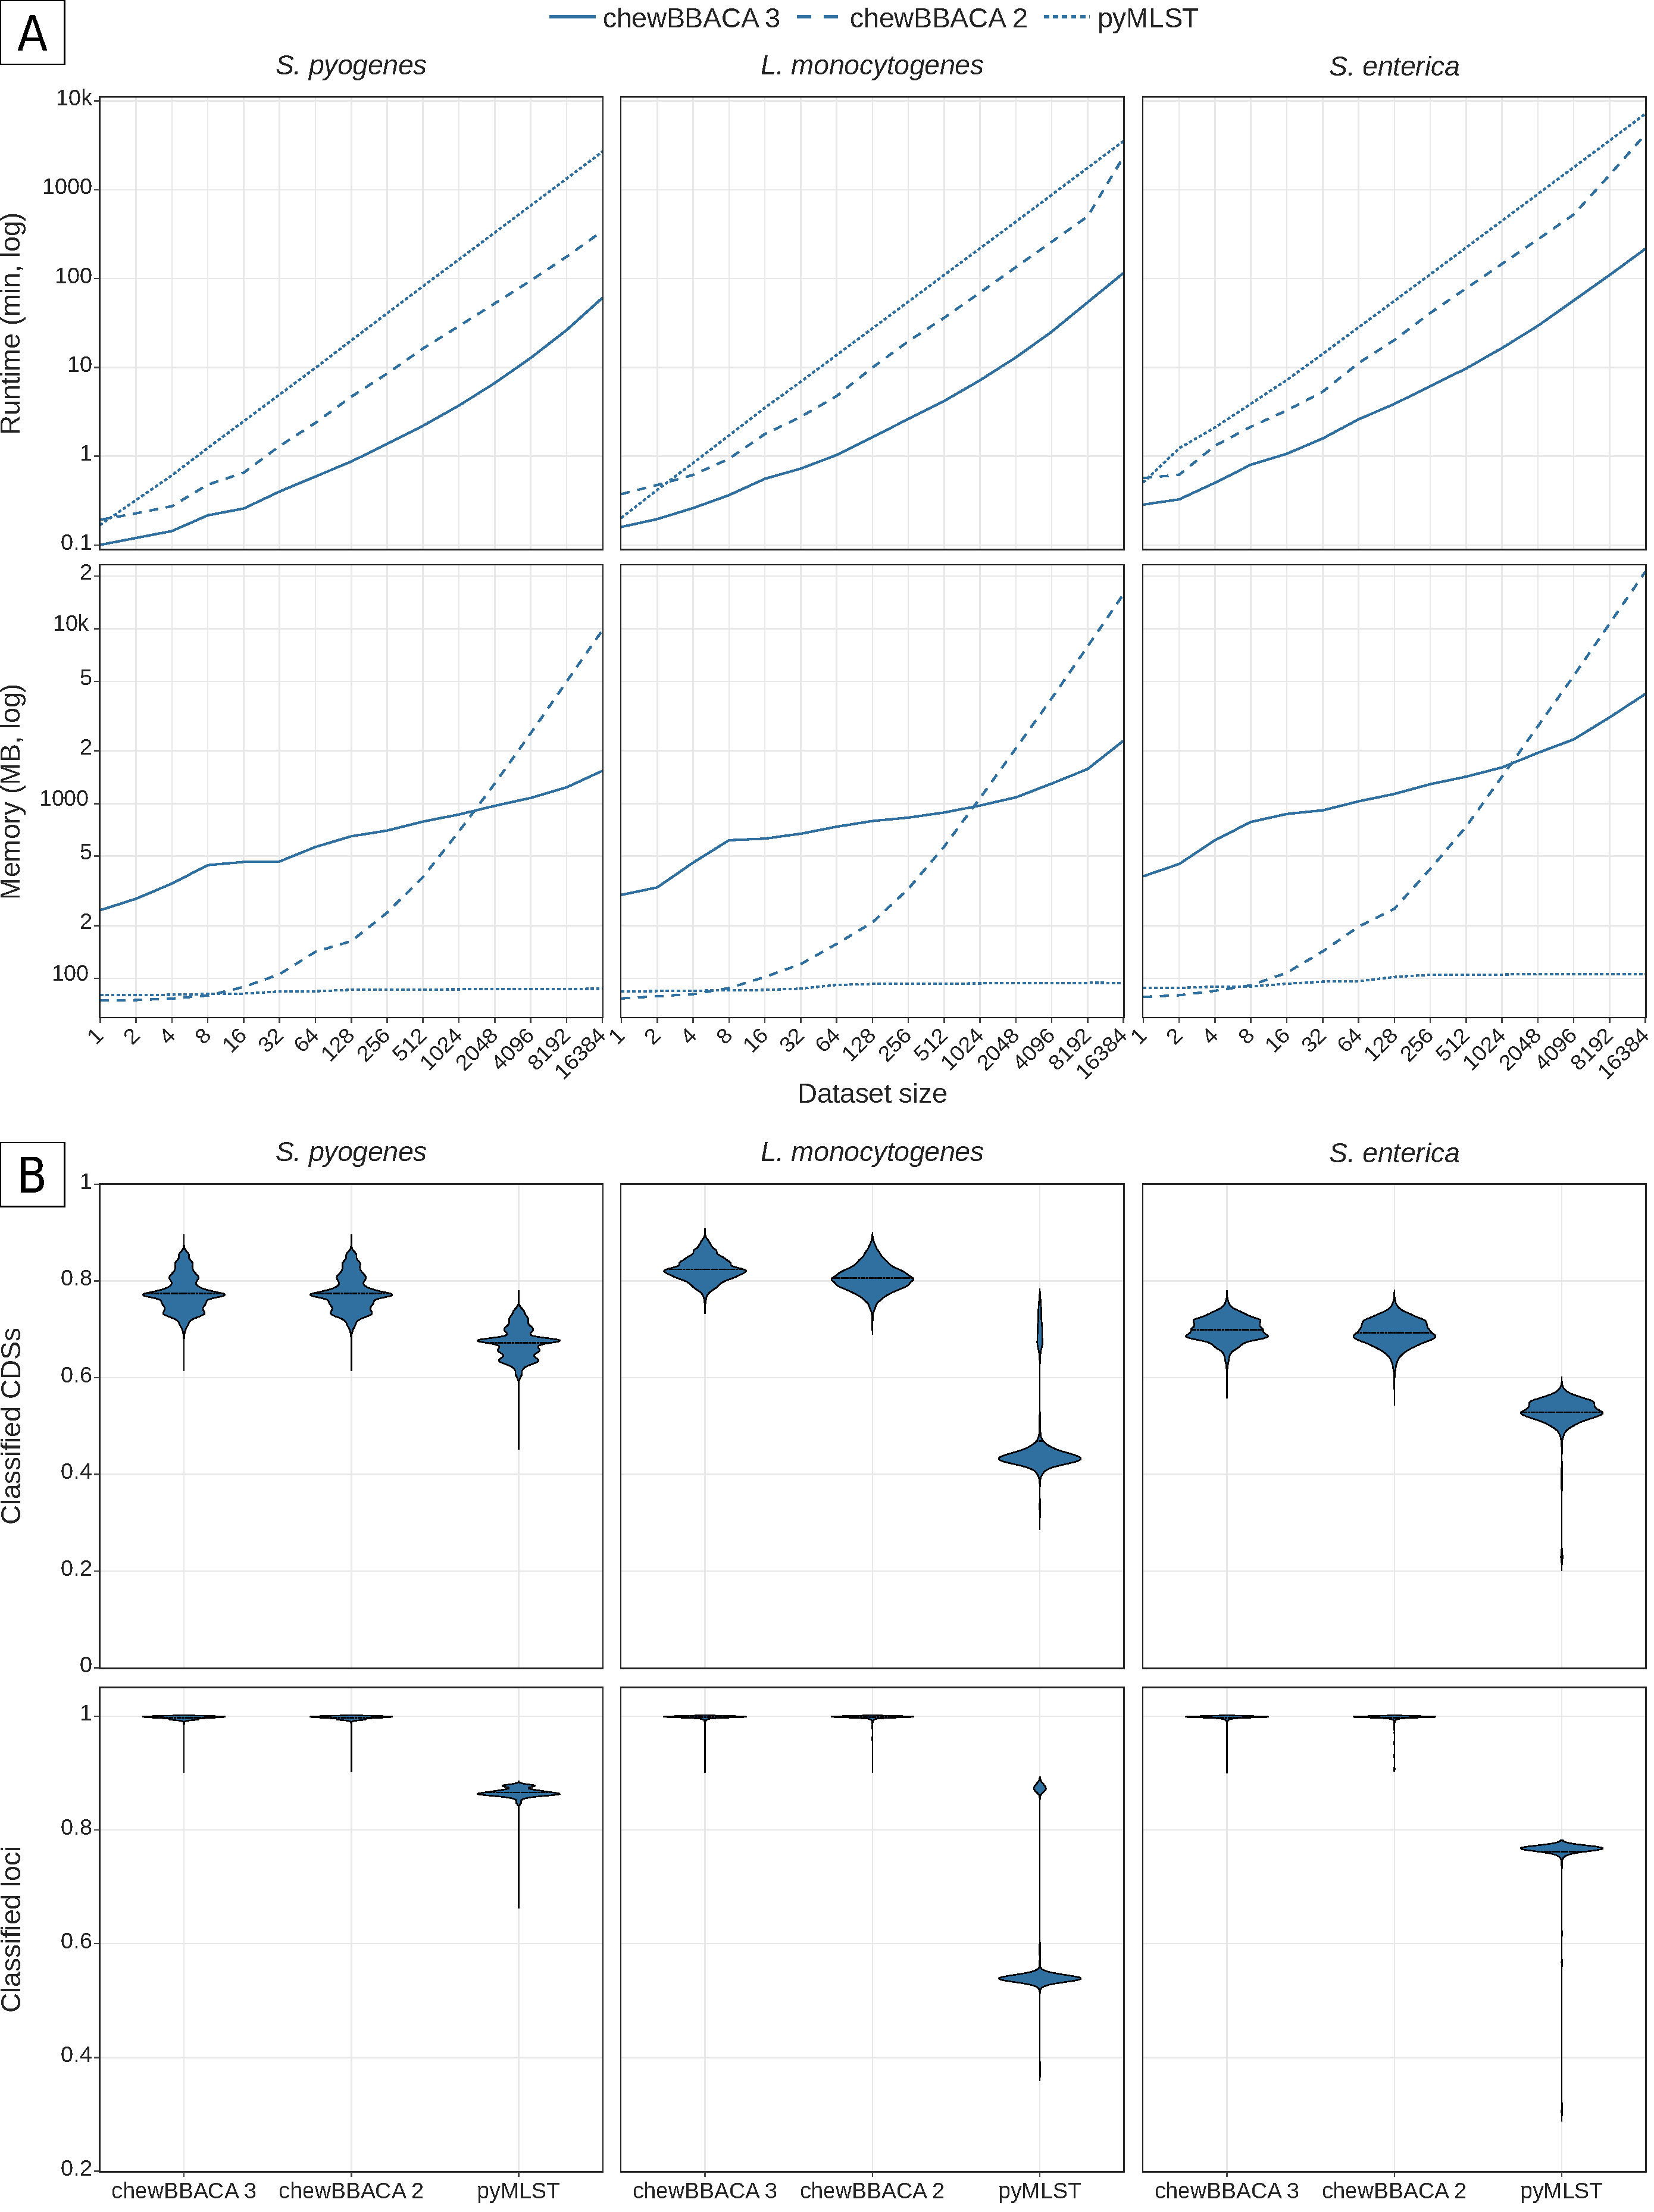
\includegraphics[angle=0,width=0.93\textwidth]{figures/chapter 2/Figure2.pdf}
    \caption{Performance comparison of chewBBACA 3, chewBBACA 2 and pyMLST. (A) Runtime and peak memory usage comparison for the allele calling of datasets with a varying number of genomes (from 1 to 16,384) for three bacterial species: Streptococcus pyogenes, Listeria monocytogenes, and Salmonella enterica. The benchmark was performed with five replicates per dataset size, except for the complete dataset (n=16384). The values shown are the mean of the replicate values for each dataset. Runtime was measured as the elapsed real time in minutes (logarithmic scale). Peak memory usage was measured as the maximum resident set size in MB (logarithmic scale). (B) Proportion of strain CDSs and schema loci classified for the complete datasets (n=16384). The proportion of classified CDSs corresponds to the number of CDSs classified by each tool divided by the total number of CDSs predicted for each strain by Pyrodigal. The proportion of classified loci corresponds to the number of schema loci identified by each tool divided by the total number of schema loci.}
    \label{fig:chap2_figure2}
\end{figure*}

Additionally, the novel minimizer-based clustering matches the remaining CDSs to the most similar schema loci, reducing comparisons between dissimilar sequences. These two steps contribute the most to the increased speed compared to chewBBACA 2 and pyMLST, which process each genome separately and additionally do not take advantage of multiprocessing settings as efficiently as chewBBACA 3. Regarding peak memory usage (Figure 2A and Table S8, Additional File 2), chewBBACA 3 used, on average, 8.6- to 1.1-fold more memory than chewBBACA 2 for datasets with up to 1,024 strains. The inverse was observed for larger datasets, with chewBBACA 2 using 1.1- to 6.9-fold more memory than chewBBACA 3. Compared to pyMLST, chewBBACA 3 used 3.1- to 40-fold more memory. pyMLST maintains low memory usage irrespective of dataset size but is single-threaded and only supports the addition of one strain per command, which limits its scalability. chewBBACA 3 enables considerably faster analyses while keeping memory usage in check to allow large-scale analysis without needing high-performance computing infrastructures. While comparing results using the entire wgMLST schema would further highlight chewBBACA 3’s efficiency and accuracy, time and memory constraints related to running chewBBACA 2 and pyMLST under the same conditions invalidated such comparison.

The thoroughness of the allele calling in chewBBACA 3 can be controlled through four execution modes (Figure S6, Additional File 1). Mode 1 identifies exact matches at the DNA level between the genomes’ CDSs and the schema alleles. Mode 2 adds exact matching at the protein level, enabling the identification of novel alleles with synonymous substitutions. Mode 3 proceeds to clustering and intracluster alignment to identify similar alleles based on the BSR threshold. Mode 4, the default, runs the complete process to classify as many CDSs as possible and potentially selects new representative alleles, preparing the schema to better identify future novel alleles. Modes 1 and 2 offer a 4.7-fold speedup over the default mode (Figure S13, Additional File 1 and Tables S9 and S10, Additional File 2), but their capacity for allele identification is limited to only modestly divergent alleles. This makes them appropriate for applications where a less accurate but much faster strain discrimination is sufficient, or for faster allele calling with schemas that already capture most of a species’ diversity for the set of loci that make up those schemas, as is the case for many publicly available cgMLST schemas. Mode 3 provides similar accuracy to the default mode in less time, with a more significant reduction in runtime for larger schemas and more diverse datasets. Mode 4 offers greater sensitivity to identify the most divergent alleles and select new representative alleles to add to schemas, which is essential to increase the diversity captured by a schema, especially in the initial phase of schema development. For schemas that already include representative alleles that capture a species diversity, Mode 3 and Mode 4 may only differ in the number of special classifications attributed, with Mode 4 identifying more.

chewBBACA 2 added new alleles to schemas automatically, not providing any option for users to prevent the allele call process from changing an existing schema. chewBBACA 3 includes the --no-inferred option to control this behaviour. This option can be helpful in several scenarios, including: updating schemas only periodically, in applications where frequent schema updates can compromise the reproducibility of the allele calling; classifying genomes from closely related species to identify similar loci; and avoiding adding spurious alleles to a schema when there's uncertainty about the quality level of the genome assemblies being analyzed.

\subsection{Comprehensive allele calling for more accurate and detailed results} \label{ssec:results_discussion_ssec3}

We evaluated the allele calling results for the complete dataset of each of the three species chosen (consisting of 16,384 genomes) to measure the comprehensiveness of chewBBACA 3's results and compare it against chewBBACA 2 and pyMLST. Results were compared at the core and accessory genome levels, based on a locus presence threshold of 95\%, of the cgMLST schemas defined above. Concordance was measured by comparing the pairwise Jaccard distances computed based on the allelic profiles. The core and accessory loci sets determined based on chewBBACA 3’s and chewBBACA 2’s results were highly similar, sharing over 99\% and 95\% of the loci at the core and accessory levels, respectively (Table S11, Additional File 2). The pairwise Jaccard distances were strongly correlated and near the identity line, indicating high concordance between the results (Figure 3), with the pairwise allelic distances computed by both tools differing by 0 to 6 differences on average (Figure S14, Additional File 1). The core loci sets determined based on pyMLST’s results were considerably smaller, containing 42\% to 80\% of the schema loci, compared to over 94\% for chewBBACA 3. The reduced number of core loci identified by pyMLST is related to an inconsistent identification of some loci in each species. This is partly due to the default identity and coverage thresholds used by pyMLST, which are more stringent than the default BSR threshold used by chewBBACA and do not allow for the same degree of allele sequence variability. Moreover, pyMLST uses a single representative allele per locus to search for matches, whereas chewBBACA 3 can add new representative alleles to schemas to better capture locus diversity. pyMLST's accessory loci sets were 4- to 11-fold larger than chewBBACA 3's (Table S11, Additional File 2). The accessory pairwise Jaccard distances were weakly correlated, except for S. pyogenes, and the pairwise allelic distances differed by 49 to 141 differences on average. While chewBBACA 2 generates highly comparable results to chewBBACA 3, pyMLST yields considerably different loci sets and pairwise distances, indicating it is not easily comparable to chewBBACA 3. This highlights the importance of the choice of method for cg/wgMLST and how the differences detected and distance thresholds defined by different methods may not be equivalent.

chewBBACA 3 classified a similar number of CDSs than chewBBACA 2 for S. pyogenes and 1.8\% and 0.7\% more CDSs for L. monocytogenes and S. enterica, corresponding to an average of 56 and 33 more CDSs per strain (Figure 2B and Table S12, Additional File 2). chewBBACA 3 classified 10\% to 35\% more CDSs than pyMLST, 177 to 1078 more CDSs per strain, on average. chewBBACA 3 and chewBBACA 2 identified over 99\% of the schema loci in all strains, while pyMLST identified between 58\% and 87\% loci (Figure 2B). Running chewBBACA 3 in mode 3 provided nearly identical results to the default mode. Modes 1 and 2 classified 4\% to 6\% fewer CDSs and identified 6\% to 7\% fewer loci than the default mode, respectively, performing worse if many of the strains’ alleles were not equal or highly similar to the alleles in the schemas (Figures S15 and S16, Additional File 1).

\begin{figure*}[h!]
    \centering
    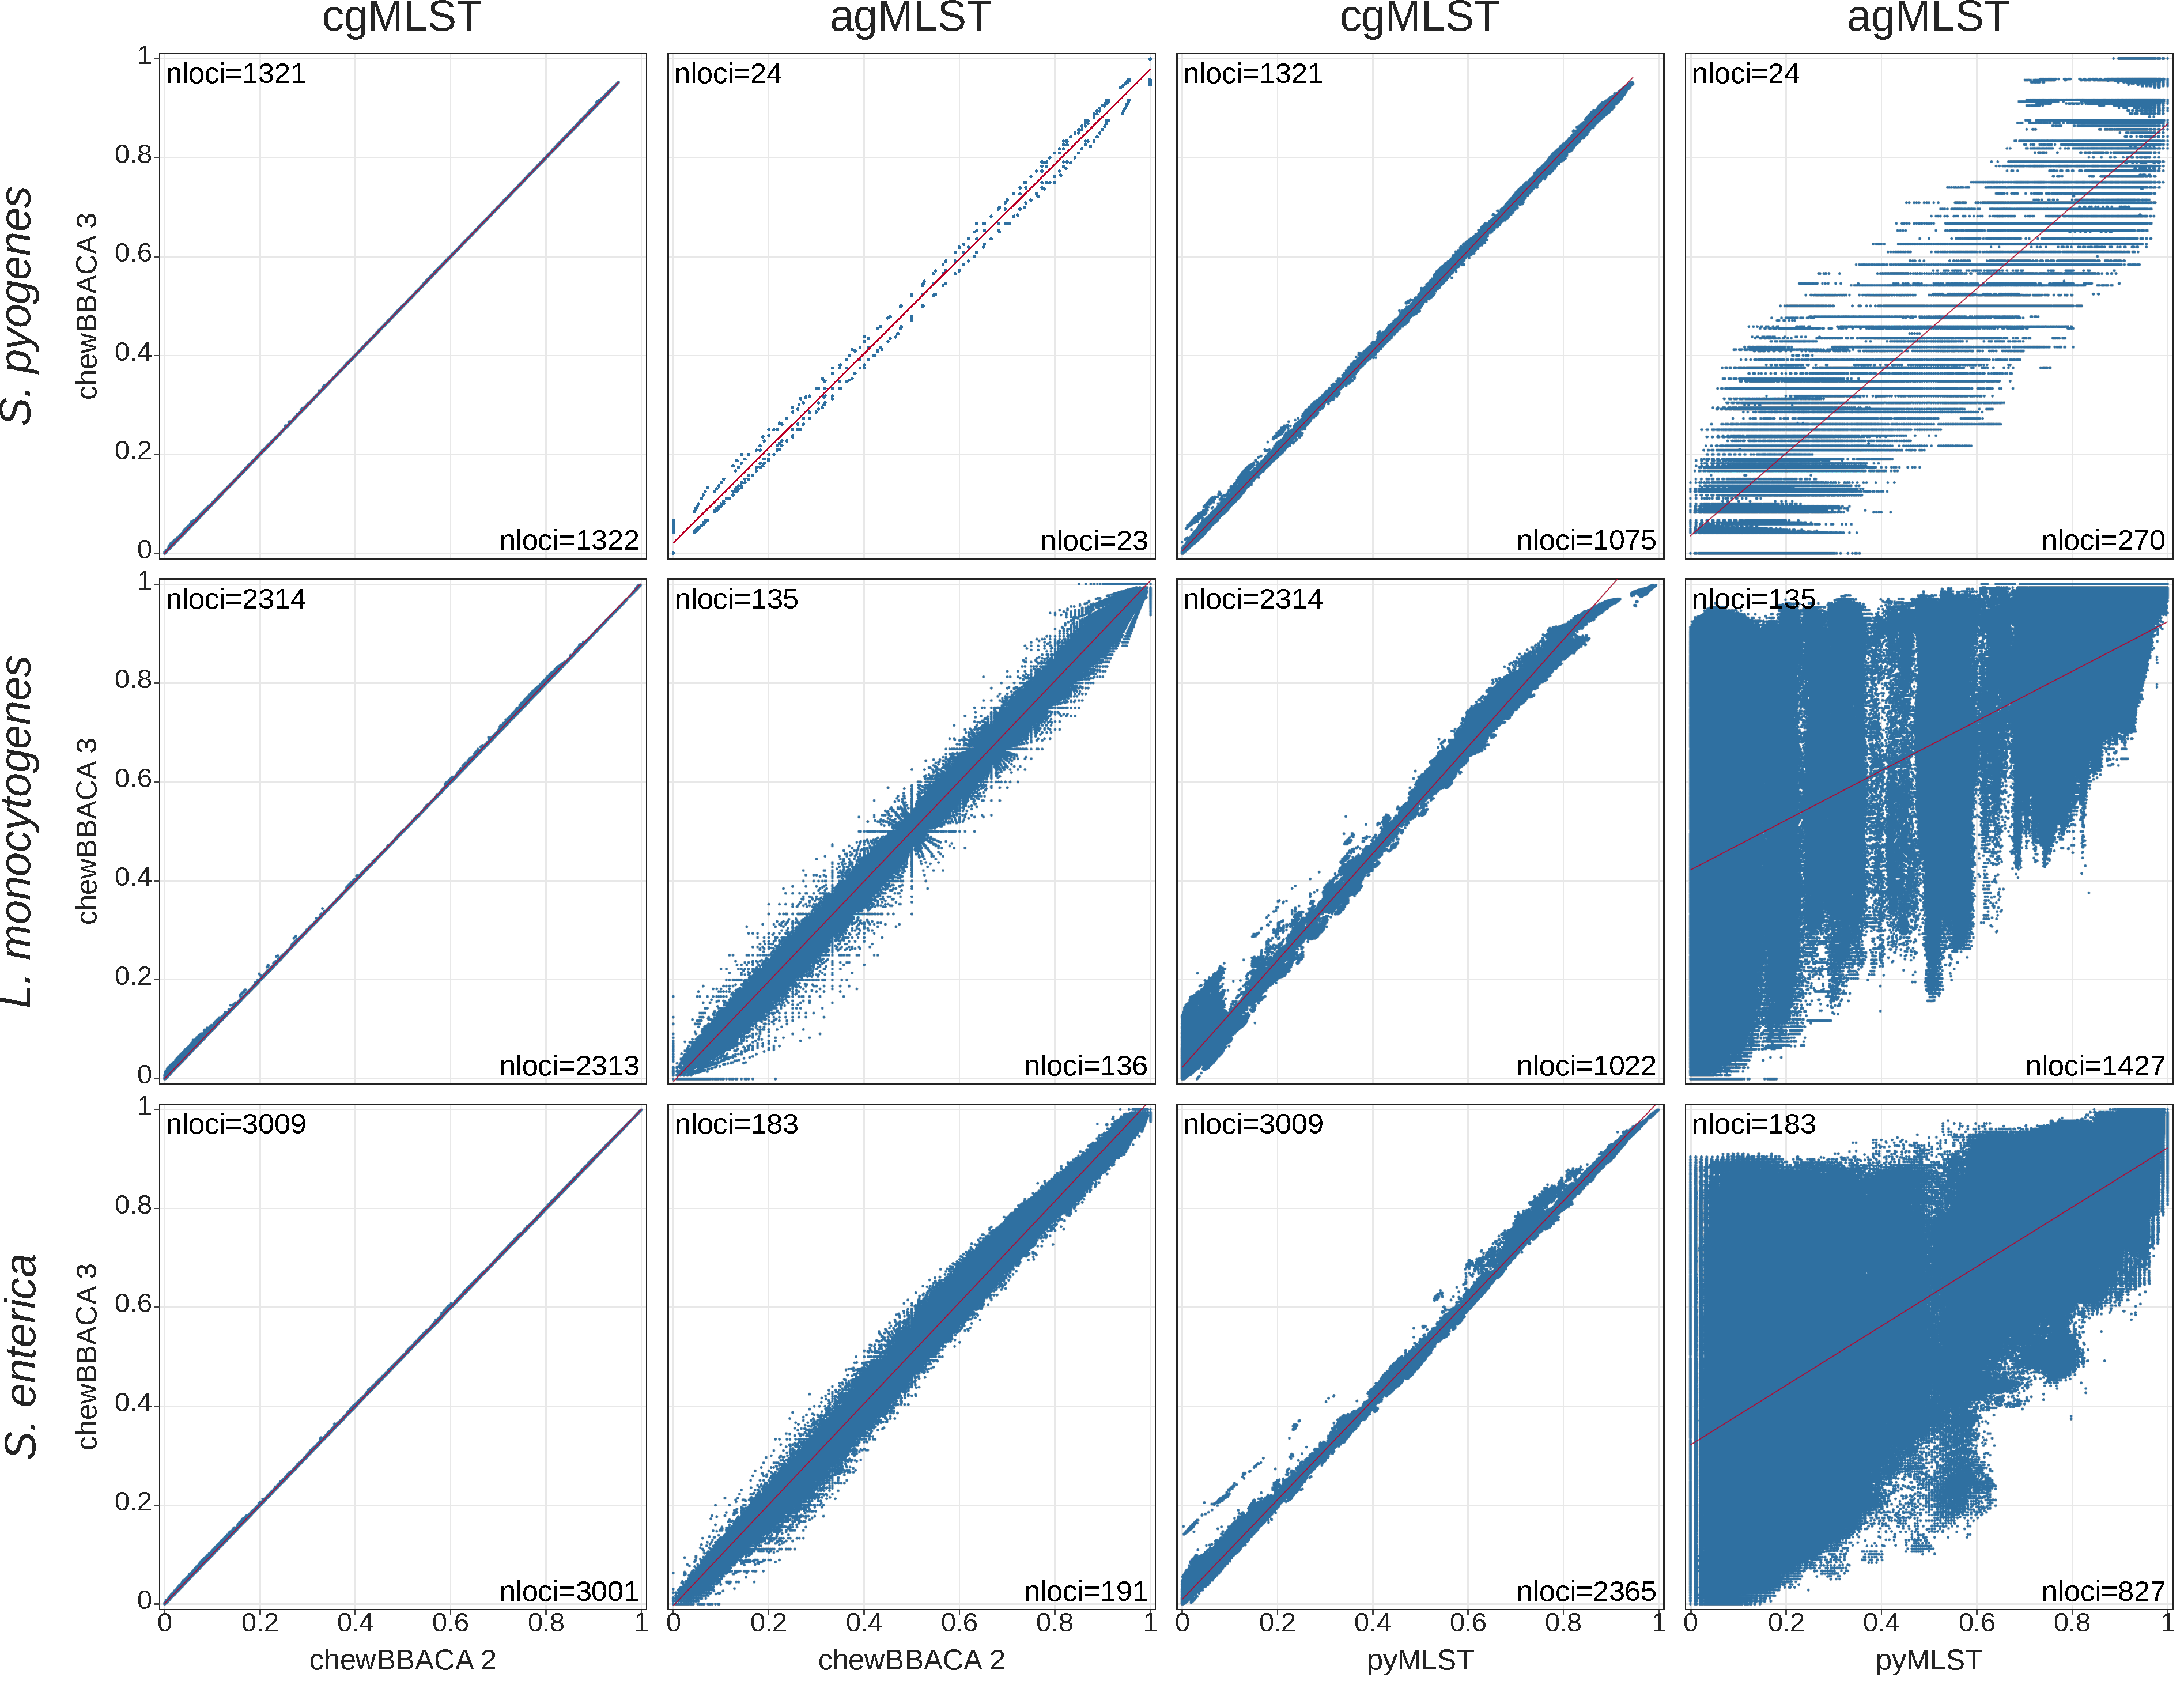
\includegraphics[angle=0,width=\textwidth]{figures/chapter 2/Figure3.pdf}
    \caption{Comparison of the core (cgMLST) and accessory (agMLST) pairwise Jaccard distances. The pairwise Jaccard distances computed based on chewBBACA 3's allele calling results for the complete datasets (n=16,384 genomes) of Streptococcus pyogenes, Listeria monocytogenes, and Salmonella enterica were compared against the the pairwise distances computed from chewBBACA 2's and pyMLST's results. The regression lines are displayed in red. The number of core or accessory loci determined based on chewBBACA 3’s results are shown in the top-left corner of the plot area. The number of core or accessory loci determined based on chewBBACA 2’s or pyMLST’s results are shown in the bottom-right corner of the plot area.}
    \label{fig:chap2_figure3}
\end{figure*}

Compared to chewBBACA 2, chewBBACA 3 identifies special classifications more accurately (Figures S17-S19, Additional File 1 and Table S13, Additional File 2). The identification of paralogous loci was improved by introducing the PAMA classification (Figure S3, Additional File 1) for CDSs that match multiple loci and subdividing the NIPH classification into NIPHEM and NIPH to differentiate between multiple exact matches or a combination of exact and inexact matches (Figure S2, Additional File 1). chewBBACA 3 displays greater sensitivity for detecting multiple matches, leading to more NIPH and NIPHEM classifications than chewBBACA 2, which, in some cases, would detect a single exact match and fail to identify additional inexact matches. The PLOT classification, used by chewBBACA 2 to classify CDSs close to contig ends, was subdivided into PLOT5, PLOT3 and LOTSC to indicate if a CDS is close to the 5'-end, 3'-end, or both (Figure S1, Additional File 1). New output files include the genomic coordinates for the CDSs predicted for all input genomes and relevant classification statistics per genome and locus. The DNA sequences of the CDSs assigned special classifications or not classified can be stored in FASTA files by providing the --output-missing and --output-unclassified options, respectively. These changes improve the granularity of the results to facilitate downstream analyses, such as identifying low-quality inputs, paralogous loci, more divergent alleles, and potential new loci to add to schemas.

Another known issue when using cg/wgMLST approaches is that allelic profiles generated with schemas that do not share the same allele nomenclature are not directly comparable. To enable the comparison of results generated with different schemas, chewBBACA 3 includes the --hash-profiles option that hashes allele sequences to generate hashed allelic profiles. Since the same allele sequence will always result in the same hash value, the allelic profiles can be compared independently of the nomenclatures used by the schemas allowing also greater data privacy. chewBBACA 3 uses the SHA256 algorithm included in Python’s hashlib module by default, but users can select any of the algorithms included in that module or the zlib module.

\subsection{Interactive reports for comprehensive wg/cgMLST schema and allele call results analyses} \label{ssec:results_discussion_ssec4}

The schemas and allele calling results generated by chewBBACA 3 can be a source of valuable data for in-depth analyses that explore the loci diversity captured by a schema and the relatedness of strains of interest. We developed modules that enable a local, scalable and comprehensive analysis of cg/wgMLST schemas and results through interactive reports to support users in performing common downstream analyses to more easily reach an informed decision. To showcase the utility of the reports' functionalities, we analysed 264 S. pyogenes emm1 strains, including strains from the recently emerged M1UK and M1DK lineages \citep{lynskey_emergence_2019, johannesen_increase_2023}, and describe how some of the reports’ components can help identify relevant features to distinguish the lineages.

The SchemaEvaluator (Figure S20, Additional File 1) module evaluates cg/wgMLST schemas created with chewBBACA or from external sources to create an interactive report with detailed information about the schema composition. This module had been introduced in chewBBACA 2, however it ceased functioning due to dependency issues. The module was reimplemented and expanded in chewBBACA 3. The main page of the report includes charts that allow exploring the number of alleles and the allele size variation per locus. The module accepts a file with loci annotations to facilitate the identification of loci of interest. For example, the annotations determined by the UniprotFinder module (Figure S21, Additional File 1) for the S. pyogenes schema can be added to a data table to identify which schema loci have the lineage-defining single-nucleotide polymorphisms (SNPs) of the M1UK (Figure 4A) and M1DK lineages. Another data table displays the results of the allele integrity analysis, which identifies classes of invalid alleles per locus (e.g. incomplete CDSs, presence of ambiguous bases, absence of start and stop codons, in-frame stop codons, and minimum and locus-specific size thresholds). This can be used to identify problematic loci or loci with unusual variability of size.

\begin{figure*}[h!]
    \centering
    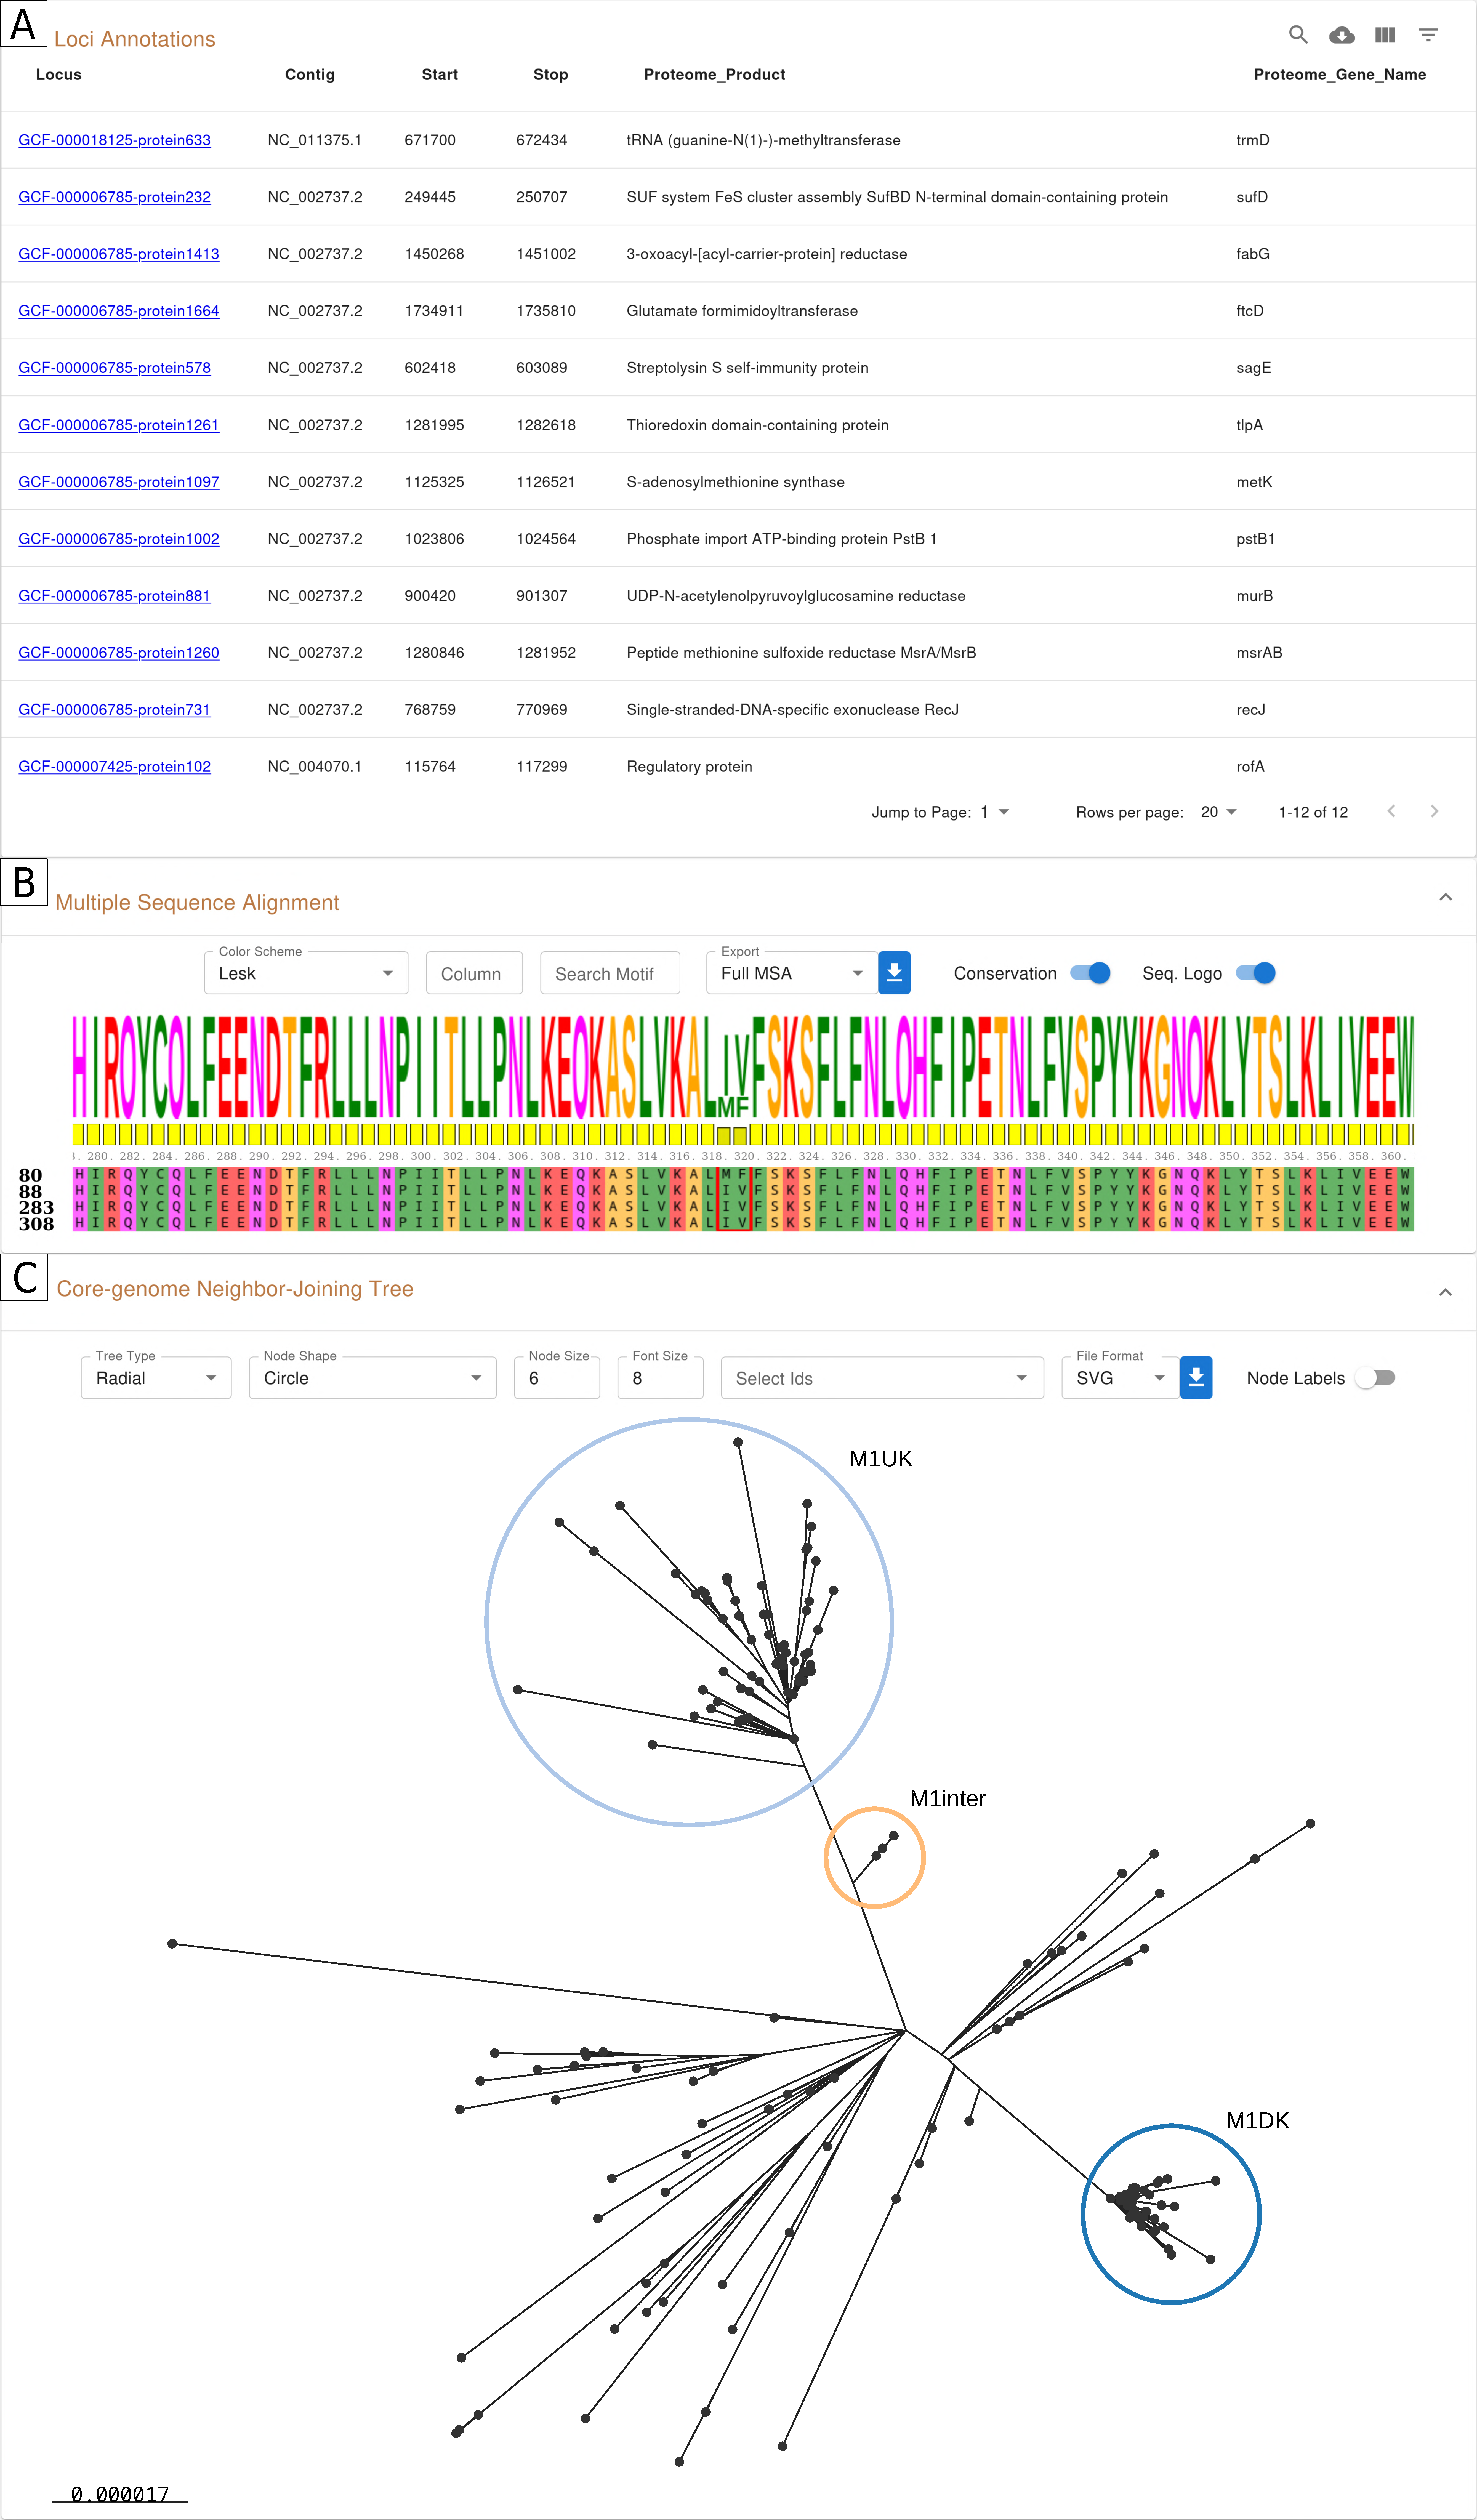
\includegraphics[angle=0,height=0.92\textheight]{figures/chapter 2/Figure4.pdf}
    \label{fig:chap2_figure4}
\end{figure*}
\vspace*{-6mm}
\begin{center}
    \emph{(Caption on next page.)}
\end{center}
\begin{figure*}[h!]
    \caption{Report components generated for the analysis of the \textit{S. pyogenes} schema and lineage strains. (A) Datatable component of the report generated by the \textit{SchemaEvaluator} module including the annotations determined by the \textit{UniprotFinder} module for 12 schema loci containing lineage-defining SNPs for the M1UK lineage. (B) Component of the \textit{SchemaEvaluator} module including a Multiple sequence alignment (MSA) of the rofA translated alleles identified in the MGAS5005 reference strain (allele 80) and the M1UK strains (alleles 88, 283, and 308). Two amino acid differences caused by two SNPs in the rofA alleles of the M1UK strains are highlighted in red. (C) Component of the \textit{AlleleCallEvaluator} module including a Neighbor-Joining tree computed with FastTree from the core loci MSA. The groups of strains belonging to the M1UK (light blue), M1inter (light orange), and M1DK (dark blue) lineages are highlighted. The full reports are available on Zenodo \citep{mamede_supplementary_2025}.}
\end{figure*}

The \textit{-{}-loci-reports} option provides a more detailed analysis of each locus through dedicated locus pages, accessible by clicking on the loci identifiers in the main report data tables. Each locus page contains charts for the allele size distribution, sequence size per allele and number of DNA alleles for each distinct protein. A multiple sequence alignment (MSA) computed with MAFFT \citep{katoh_mafft_2013} for the translated alleles allows identifying shared regions and differences caused by point mutations or indels. For example, the non-synonymous effect of two SNPs in the rofA gene used to define the M1UK lineage can be identified using the MSA by comparing the reference allele with those identified in M1UK strains (Figure 4B). The guide tree created by MAFFT is displayed with Phylocanvas.gl \citep{abudahab_phylocanvasgl_2021} to help identify groups of similar or divergent alleles. To provide a convenient way to identify and copy the DNA and protein sequences of the alleles, users can use the --add-sequences option, which adds code editor components containing the DNA and protein sequences to each locus’ page.

A report with a detailed analysis of the allele calling results is obtained by running the AlleleCallEvaluator module (Figure S22, Additional File 1). The report includes data tables with summary statistics and bar charts with the classification counts per strain and locus to explore the classification results and aid in identifying low-quality genomes (e.g. misassembled or contaminated genomes) and problematic loci (e.g. loci with a high number of special classifications). An interactive analysis of loci presence-absence is performed through a heatmap component that enables identifying the set of core loci or loci specific to certain groups of strains. Similar strains can be identified through another heatmap component that displays the matrix of pairwise core allelic distances and enables searching for similar strains based on a distance threshold. The last component in the report displays a Neighbor-Joining tree computed with FastTree 2 \citep{price_fasttree_2010} from the core loci MSA. This component allows exploring phylogenetic relationships to identify groups of similar strains. For instance, the NJ tree from the analysis of the S. pyogenes strains allows identifying the groups of strains corresponding to each lineage of the M1 group (Figure 4C).

The reports' components include features to sort, select, search, and export data in tabular format, in the case of data tables, or as SVG files, in the case of charts or trees. Some files necessary to create the components, such as the ones containing the matrix of pairwise core allelic distances and the core loci MSA, are provided in the report's folder to allow users to perform custom analyses if desired. The reports are easily shared by simply compressing the report's folder and sharing the resulting archive. The interactive reports created with the SchemaEvaluator and AlleleCallEvaluator modules for the analysis of the S. pyogenes strains are available on Zenodo \citep{mamede_supplementary_2025}.

\section{Conclusions} \label{sec:conclusions}

chewBBACA 3 constitutes an efficient, scalable, and comprehensive solution for wg/cgMLST. The options it provides for schema setup enable users to quickly create schemas from larger collections of genome assemblies or CDS data to capture more of the diversity of a bacterial species, or to adapt or import existing schemas created in other platforms or available in Chewie-NS to promote interoperability. The combination of alignment-based and alignment-free approaches allow for efficient and accurate allele calling, making it suitable for integration into workflows that process sample batches of any size, from sequential processing of single samples to vast genome collections for species-level population analyses. chewBBACA 3 classifies more schema loci and CDSs than the compared methods, potentially providing superior strain discrimination for surveillance and outbreak investigation. The high level of agreement with chewBBACA 2's results, while providing expanded classifications and richer results, facilitates the transition to the latest chewBBACA version. Comparisons with other wg/cgMLST methods should take into account that algorithmic differences between methods, parameter values, and input data quality can greatly affect the resolution and accuracy of the results, which might hinder results comparison and in some cases even lead to fundamentally different conclusions. The reports for schema and allele call evaluation allow a comprehensive and local analysis of locus diversity and strain similarity, enabling scalable and private analyses of the results and reducing the need to combine several tools or develop custom solutions to more fully explore the potential of wg/cgMLST schemas. The integration of chewBBACA 3 into wg/cgMLST workflows will help to further democratize wg/cgMLST by providing broader access to large-scale and detailed analyses to perform focused population studies or facilitate reaching an informed decision in outbreak or transmission investigations.

\section{Methods} \label{sec:methods}

\subsection{Download and selection of complete and draft genome assemblies} \label{ssec:methods_ssec1}

Complete and draft genome assemblies annotated as \textit{Streptococcus pyogenes}, \textit{Listeria monocytogenes} and \textit{Salmonella enterica} were downloaded with the NCBI Datasets command-line tools v16.12.0 \citep{oleary_exploring_2024} on September 9, 2023. The complete genomes were downloaded from the NCBI RefSeq database \citep{sayers_database_2022} using the –assembly-source “RefSeq” and –assembly-level complete options. The draft genome assemblies were downloaded from the NCBI GenBank database \citep{sayers_database_2022} using the –assembly-source “GenBank” option. The –exclude-atypical and –mag exclude options were used in both cases. The number of draft genome assemblies for \textit{S. pyogenes} available from GenBank was insufficient to create the complete dataset (n=16384) for the benchmark. Due to that, draft genome assemblies annotated as \textit{Streptococcus pyogenes} were also downloaded from a collection of 661K genomes available on the European Nucleotide Archive (ENA) \citep{blackwell_exploring_2021}. MLST v2.23.0 \citep{jolley_bigsdb_2010, seemann_mlst_nodate} was used to determine the Sequence Type (ST) for all assemblies. Assemblies without a known ST or assigned an ST from a different species, indicating possible misannotation, were excluded. A custom Python script was also used to filter out assemblies based on a maximum number of contigs of 100, a maximum number of ambiguous bases of 1000, and a minimum and maximum genome size. The minimum and maximum genome size values were defined based on the \textit{min\_ungapped\_length} and \textit{max\_ungapped\_length} values in the “species\_genome\_size.txt” file available on NCBI’s FTP on September 9, 2023 (\url{https://ftp.ncbi.nlm.nih.gov/genomes/ASSEMBLY_REPORTS/}) \citep{sayers_database_2022}.

\subsection{Dataset creation} \label{ssec:methods_ssec2}

The selected draft genome assemblies were subsampled to create datasets to evaluate the performance of chewBBACA 3, chewBBACA 2 and pyMLST. The pairwise average nucleotide identity (ANI) distances for each species’ selected draft genomes were computed with Skani v0.2.1 \citep{shaw_fast_2023}. To factor in the aligned genome fraction, weighted ANI values were computed by multiplying the ANI values by the mean of the query and reference aligned fractions. The weighted ANI values were ordered to select a set of 16,384 genomes that maximized the average pairwise distance. Smaller datasets were created by randomly sampling this dataset, starting by selecting 1 genome and doubling the dataset size until reaching a dataset size of 8,192. Five replicates were created for each dataset size. The complete datasets with 16,384 genomes were compressed with AGC v3.0 \citep{deorowicz_agc_2023} to allow efficient storage and fast genome retrieval based on lists of genome identifiers.

\subsection{Creation of wg/cgMLST schemas} \label{ssec:methods_ssec3}

A total of 260, 309 and 1,326 complete genomes for \textit{Streptococcus pyogenes}, \textit{Listeria monocytogenes} and \textit{Salmonella enterica}, respectively, were selected for schema creation. wgMLST schema seeds were created with the \textit{CreateSchema} module available in chewBBACA v3.3.6 and compared against the schema seeds created by the previous \textit{CreateSchema} implementation, available in chewBBACA v2.6.0 \citep{silva_chewbbaca_2018}. The schema creation processes used a minimum sequence length value of 0 (\textit{--l 0}) and the Prodigal \citep{hyatt_prodigal_2010} training files bundled with chewBBACA. The schema seeds created by both versions were compared based on a BSR $\geq0.6$ and a proportion of shared minimizers $\geq0.9$ to determine sets of loci shared by the schema seeds created with both versions. Schema seeds created with chewBBACA v3.3.0 were populated with the alleles identified in the complete genomes through allele calling. The results of the allele calling were used to determine the set of core loci with the ExtractCgMLST module based on a loci presence threshold of 1 (\textit{--t 1}) and create the cgMLST schemas used to evaluate the allele calling performance. The cgMLST schemas were adapted with the \textit{PrepExternalSchema} module implemented in chewBBACA v2.8.5 to create the cgMLST schemas for that version. To create equivalent databases for pyMLST \citep{biguenet_introduction_2023}, multi-FASTA files with the first representative allele for each locus in the cgMLST schemas were passed to the wgMLST create command. The wgMLST add command was used to add each complete genome to the pyMLST databases.

\subsection{External schema adaptation} \label{ssec:methods_ssec4}

The cgMLST schemas for \textit{S. pyogenes}, \textit{L. monocytogenes} and \textit{S. enterica} available on the cgMLST.org server \citep{noauthor_cgmlstorg_nodate} were downloaded on July 4, 2024. These schemas were adapted with the \textit{PrepExternalSchema} module available in chewBBACA v3.3.6 and compared against the schemas adapted with the previous \textit{PrepExternalSchema} implementation, available in chewBBACA v2.0.17.2. The representativeness of the set of representative alleles selected by the \textit{PrepExternalSchema} module was measured by aligning the representative alleles selected for each locus against all valid locus alleles based on a BSR $\geq0.6$.

\subsection{Evaluation of the allele calling results} \label{ssec:methods_ssec5}

The cgMLST schemas and datasets containing between 1 and 16,384 draft genome assemblies were used to evaluate the allele calling performance of chewBBACA v3.3.3, chewBBACA v2.8.5 and pyMLST v2.1.5. The number of distinct CDSs per dataset was computed based on the CDSs predicted by Pyrodigal v3.0.0. Runtime, peak memory usage, and the comprehensiveness of the allele calling were evaluated for all datasets. The allelic profiles for the strains classified by pyMLST were extracted from the databases with the wgMLST mlst command and converted to the format used by chewBBACA with a custom script. The allelic profiles were masked to remove the \textit{INF-} prefix from inferred alleles and to substitute all special classifications or missing values by 0. The core loci were defined with the \textit{ExtractCgMLST} module based on the complete datasets' results and a loci presence threshold of 0.95. Loci below this threshold were considered to be part of the accessory genome. The pairwise Jaccard and allelic distances were computed with a custom script based on the masked allelic profiles. The proportion of classified CDSs and identified loci are based on the total number of CDSs predicted by Pyrodigal and on the total number of loci in each schema, respectively.

\subsection{Download and analysis of \textit{S. pyogenes} \textit{emm1} strains} \label{ssec:methods_ssec6}

The genome assemblies and metadata for the \textit{S. pyogenes} strains belonging to each lineage were recovered from previous studies \citep{lynskey_emergence_2019, johannesen_increase_2023, friaes_annotated_2022}. The schema loci containing the lineage-defining SNPs were identified using BLASTp to align the translated CDSs from the MGAS5005 reference genome \citep{sumby_evolutionary_2005}, with RefSeq accession number \textit{GCF\_000011765.3}, against the translated schema alleles.

\subsection{Runtime and peak memory usage measurement} \label{ssec:methods_ssec7}

Runtime and peak memory usage were measured with the GNU time command on a desktop computer with an Intel® Core™ i7-4790 CPU, 32GB 1600 MT/s RAM, and a 1TB Samsung SSD 870 QVO. Any analysis that evaluated runtime and peak memory usage used 6 CPU cores to run chewBBACA 3 and chewBBACA 2 and 1 CPU core for pyMLST because the latter cannot use multiple cores.

\section{Availability and requirements} \label{sec:availability_and_requirements}

\noindent Project name: chewBBACA 3.\\
Project home page: \url{https://github.com/B-UMMI/chewBBACA}\\
Project documentation: \url{https://chewbbaca.readthedocs.io/en/latest/index.html}\\
Operating system(s): Linux and macOS.\\
Programming language: Python >= 3.8\\
Other requirements: BLAST+ >= 2.9.0, pyrodigal>=3.0.0, numpy~=1.24.3, scipy~=1.10.1, biopython>=1.79, plotly>=5.8.0, SPARQLWrapper>=2.0.0, requests>=2.27.1, pandas>=1.5.1\\
License: GPL-3.0\\
Any restrictions to use by non-academics: None.

\section{List of abbreviations} \label{sec:list_of_abbreviations}

\noindent ANI: average nucleotide identity\\
BLASTp: Protein BLAST\\
BSR: BLAST Score Ratio\\
CDS: coding DNA sequence\\
ECDC: European Centre for Disease Prevention and Control\\
EFSA: European Food Safety Authority\\
ENA: European Nucleotide Archive\\
GbG: gene-by-gene\\
MSA: multiple sequence alignment\\
NCBI: National Center for Biotechnology Information\\
NJ: Neighbor-Joining\\
SNP: single nucleotide polymorphism\\
SNV: single nucleotide variant\\
ST: Sequence Type\\
wg/cgMLST: whole genome and core genome multilocus sequence typing\\
WGS: whole genome sequencing

\section{Declarations} \label{sec:declarations}

\subsection{Ethics approval and consent to participate} \label{ssec:declarations_ssec1}

\noindent Not applicable.

\subsection{Consent for publication} \label{ssec:declarations_ssec2}

\noindent Not applicable.

\subsection{Availability of data and materials} \label{ssec:declarations_ssec3}

The datasets, schemas and databases created and used with chewBBACA 3, chewBBACA 2, and pyMLST, and all results generated for each section are available on Zenodo (\url{https://doi.org/10.5281/zenodo.14637859}) \citep{mamede_supplementary_2025}. The supplementary figures and tables are included in the additional files.

\subsection{Competing interests} \label{ssec:declarations_ssec4}

MR received honoraria for serving on the speakers bureau of Pfizer and Merck Sharp and Dohme and for serving in expert panels of GlaxoSmithKline and Merck Sharp and Dohme. All other authors declare they have no competing interests.

\subsection{Funding} \label{ssec:declarations_ssec5}

This work was partly supported by the ISIDORe project (funding from the European Union’s Horizon Europe Research \& Innovation Programme, Grant Agreement no. 101046133). RM was supported by the Fundação para a Ciência e Tecnologia (FCT) (grant 2020.08493.BD).

\subsection{Author’s contributions} \label{ssec:declarations_ssec6}

All authors contributed to the design of the tool. RM implemented, tested, and benchmarked the tool. PVC contributed to the implementation of the tool. RM and MR wrote the manuscript. All authors read, revised and approved the final manuscript.


%%%%

%INNUca v2.6 pipeline\footnote{\url{https://github.com/B-UMMI/INNUca/}}
%$\sim$3,500
%pATLAS tool\footnote{\url{http://www.patlas.site/}}
%\ref{tab:ch2_table_1})
%\ref{fig:chap2_figure1}
%$leq$ 7

\newpage

\section{Supplemental Material}

\begin{figure*}[h!]
    \centering
    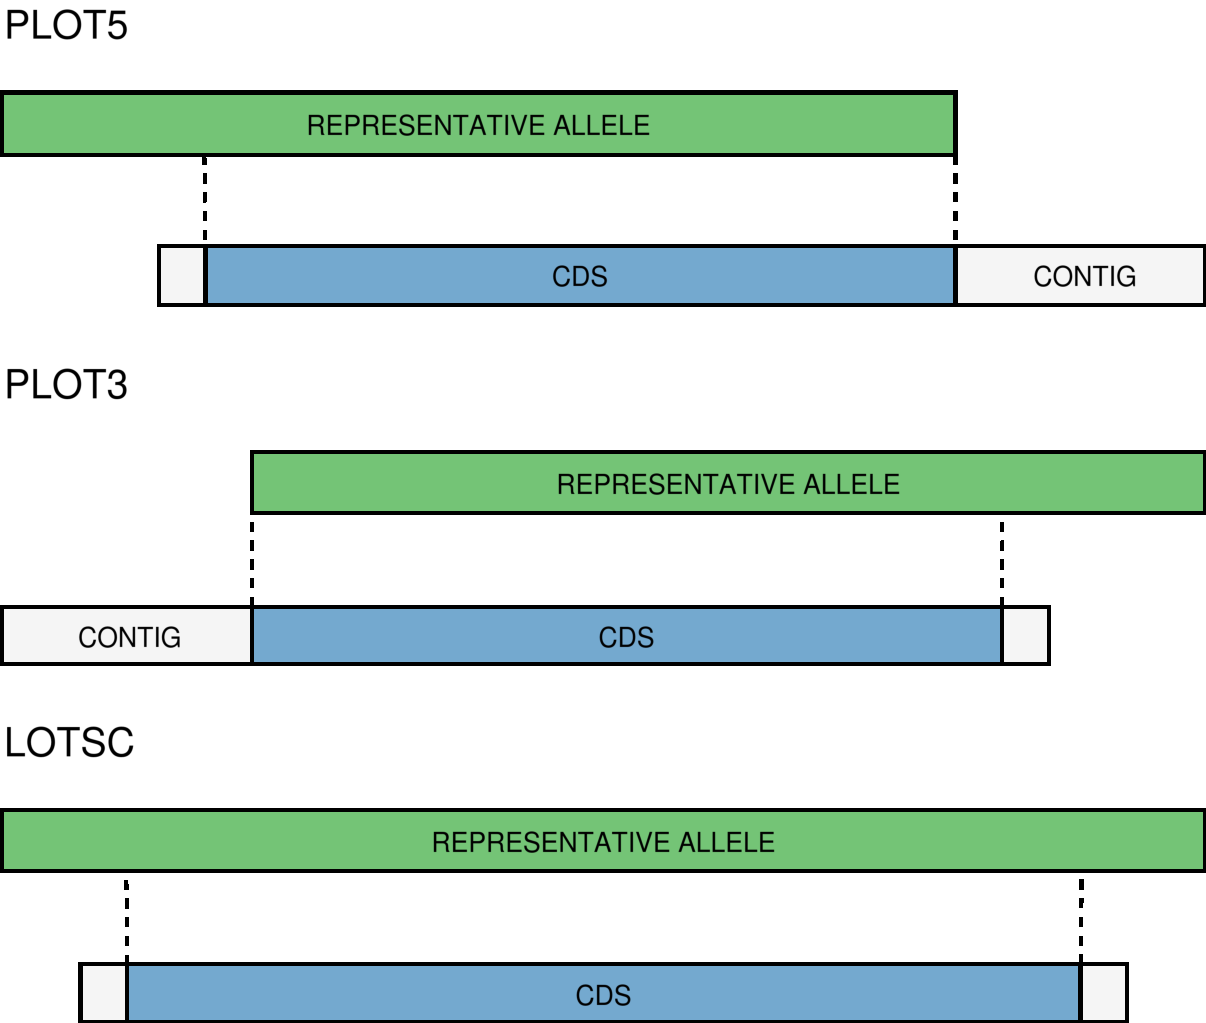
\includegraphics[angle=0,width=\textwidth]{figures/chapter 2/FigureS1.pdf}
    \caption{PLOT5, PLOT3 and LOTSC classifications. The PLOT3, PLOT5 and LOTSC classifications are related to the position of CDSs in the genomic contigs. PLOT5 and PLOT3 (Possible Locus On the Tip) - a CDS is classified as PLOT5 or PLOT3 if it is close to the contig 5’- or 3’-end and if the unaligned portion of the matched representative allele exceeds the contig end. LOTSC - a CDS is classified as LOTSC if the matched representative allele is bigger than the contig containing the CDS.}
    \label{fig:chap2_figureS1}
\end{figure*}

\newpage
\begin{figure*}[h!]
    \centering
    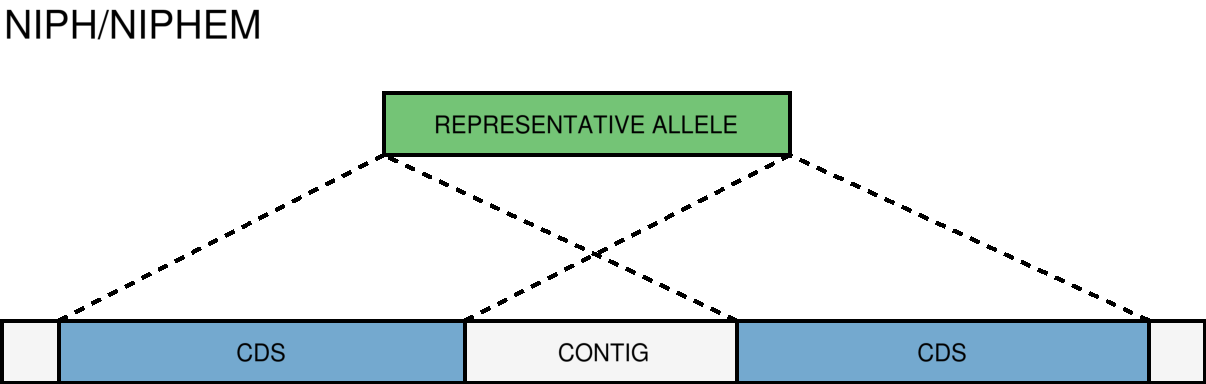
\includegraphics[angle=0,width=\textwidth]{figures/chapter 2/FigureS2.pdf}
    \caption{NIPH and NIPHEM classifications. The NIPH and NIPHEM classifications are assigned when multiple CDSs from the same genome match the same schema locus. NIPH (Non-Informative Paralogous Hit) - assigned when multiple CDSs from the same genome match a single locus. NIPHEM (Non-Informative Paralogous Hit Exact Match) - assigned when multiple CDSs from the same genome are exact matches to alleles of a single locus.}
    \label{fig:chap2_figureS2}
\end{figure*}

\newpage
\begin{figure*}[h!]
    \centering
    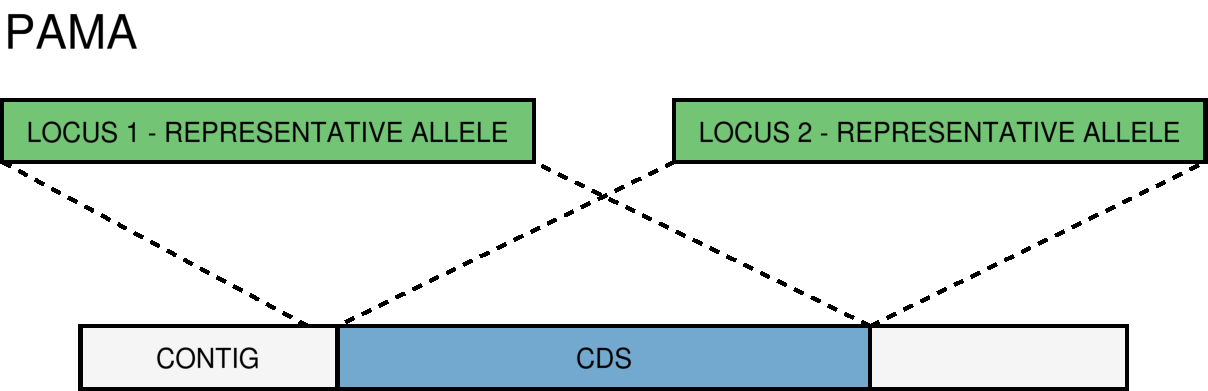
\includegraphics[angle=0,width=\textwidth]{figures/chapter 2/FigureS3.pdf}
    \caption{PAMA classification. The PAMA (PAralogous MAtch) classification is assigned when a single CDS from a genome matches multiple schema loci.}
    \label{fig:chap2_figureS3}
\end{figure*}

\newpage
\begin{figure*}[h!]
    \centering
    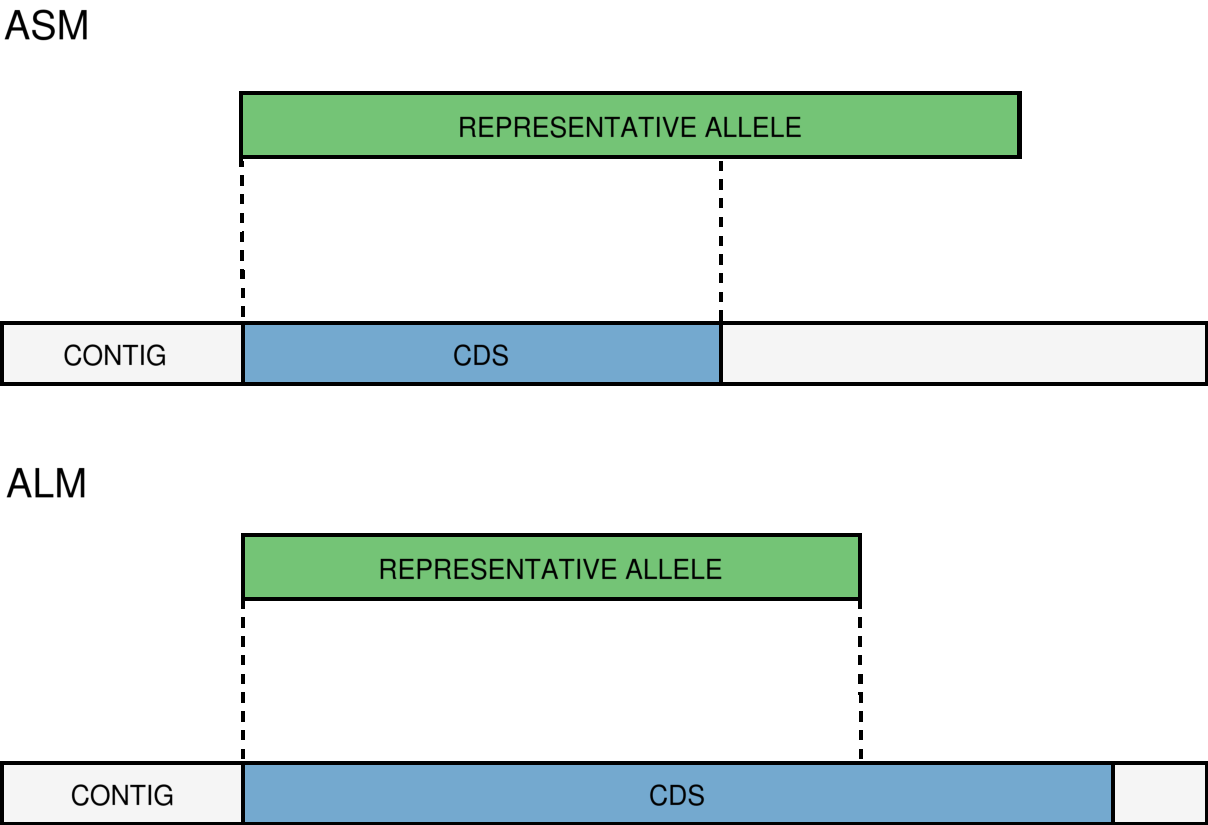
\includegraphics[angle=0,width=\textwidth]{figures/chapter 2/FigureS4.pdf}
    \caption{ASM and ALM classifications. The ASM (Allele Smaller than Mode) and ALM (Allele Larger than Mode) classifications are assigned when the size of a CDS that matches a schema locus is below or above the locus size variation interval, respectively. The default behaviour is to assign these classifications to alleles that are 20\% shorter or longer than the locus allele size mode.}
    \label{fig:chap2_figureS4}
\end{figure*}

\newpage
\begin{figure*}[h!]
    \centering
    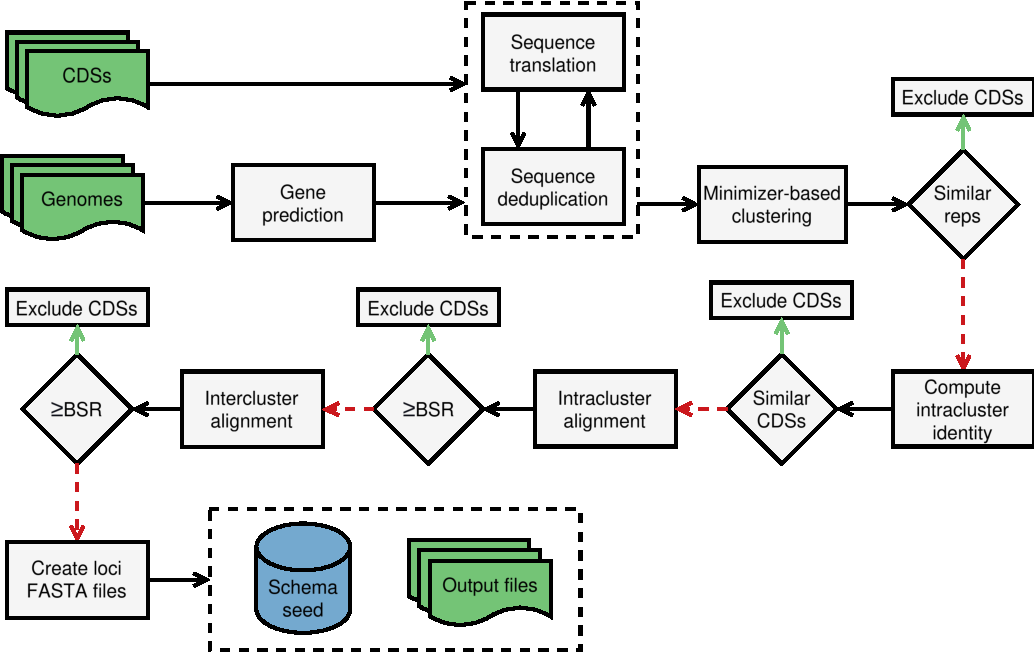
\includegraphics[angle=0,width=\textwidth]{figures/chapter 2/FigureS5.pdf}
    \caption{Diagram of the CreateSchema module. The CreateSchema module creates a schema seed based on a set of FASTA files with genome assemblies or CDSs. If genome assemblies are given, the process starts by predicting CDSs for each genome using Pyrodigal. The CDSs identified in the input files are deduplicated and translated, followed by a second deduplication step to determine the set of distinct translated CDSs. The distinct translated CDSs are clustered based on the proportion of minimizers shared with representative CDSs. The largest or one of the largest CDSs is selected as the first representative CDS. New representative CDSs are selected when CDSs share a low proportion (<0.2) of minimizers with any of the chosen representative CDSs. Non-representative CDSs that share a proportion of minimizers $\geq0.9$ with the cluster representative are considered to correspond to the same locus and are excluded from the analysis. The proportion of shared minimizers between non-representative CDSs is determined to exclude CDSs sharing a proportion of minimizers $\geq0.9$ with larger CDSs. Intracluster and intercluster alignment with BLASTp enable identifying and excluding CDSs similar to representative or larger non-representative CDSs based on a BLAST Score Ratio (BSR) $\geq0.6$. Each remaining CDS is considered to be an allele of a distinct locus. The process ends by creating a schema seed, which includes one FASTA file containing a single representative allele per distinct locus identified in the analysis. Green document icons represent input FASTA files and output files. Grey rectangle icons represent analysis steps. Diamond icons represent conditional statements, with green arrows used when the condition is met and red dashed arrows otherwise. The blue cylinder icon represents the schema seed created by the CreateSchema module.}
    \label{fig:chap2_figureS5}
\end{figure*}

\newpage
\begin{figure*}[h!]
    \centering
    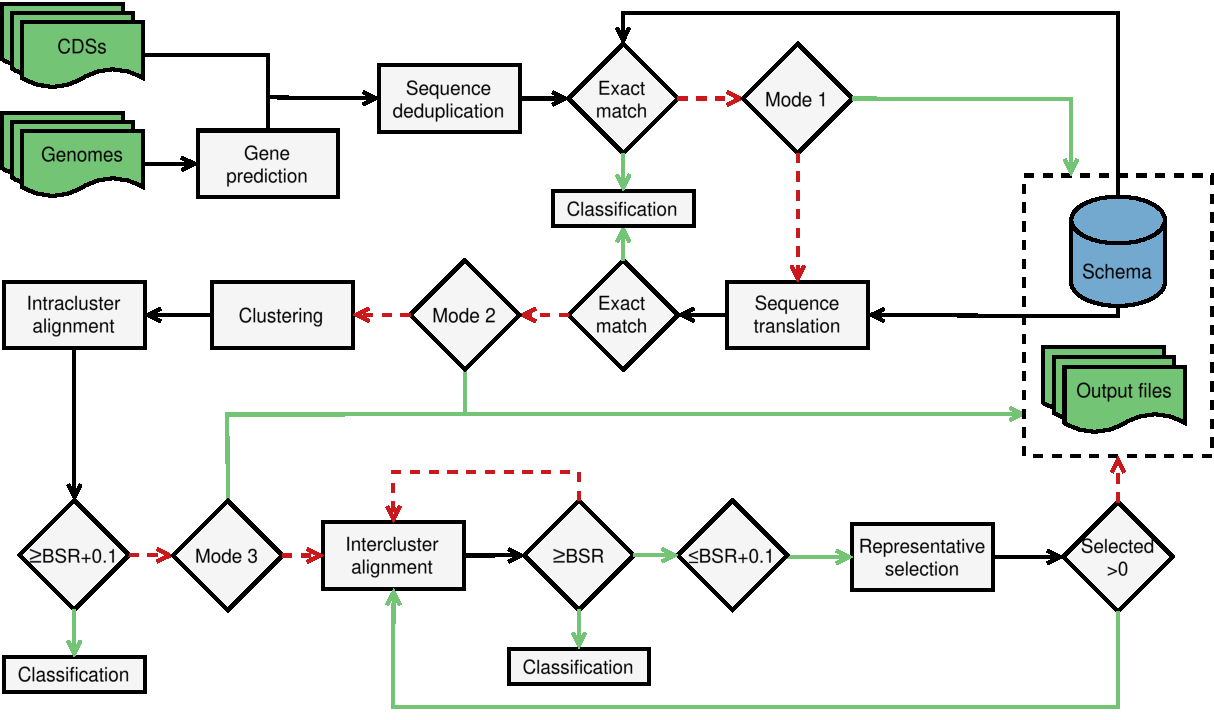
\includegraphics[angle=0,width=\textwidth]{figures/chapter 2/FigureS6.pdf}
    \caption{Diagram of the AlleleCall module. The AlleleCall module determines the allelic profiles for strains of interest. The process accepts FASTA files with genome assemblies or CDSs. If genome assemblies are given, the process starts by predicting CDSs for each genome using Pyrodigal. The CDSs identified in the input files are deduplicated and compared against the schema alleles to find and classify exact matches at the DNA level. If the process runs in mode 1, the results are evaluated to write the output files and exit. Otherwise, the CDSs that do not match any schema alleles at the DNA level are translated and matched against the translated schema alleles to find exact matches at the protein level. If the process runs in mode 2, the results are evaluated to write the output files, add new alleles to the schema and exit. Otherwise, the CDSs not classified through exact matching are compared against the schema representative alleles through minimizer-based clustering to identify CDSs that share a proportion of minimizers $\geq0.2$ with the representative alleles. Each cluster's representative allele is aligned against the clustered CDSs with BLASTp to classify CDSs based on the defined BLAST Score Ratio (BSR) value plus 0.1. At this point, if the process runs in mode 3, the results are evaluated to write the output files, add new alleles to the schema and exit. Otherwise, the representative alleles are aligned against the remaining unclassified CDSs to classify them based on the defined BSR value and identify new representative alleles whose BSR is not above the defined BSR value plus 0.1. If the process finds new representative alleles, it aligns them against the unclassified CDSs to find new matches. This process repeats until no new representative alleles are identified. When no new representative alleles are found, the process evaluates the results to create the output files, add new alleles to the schema, and exit. Green document icons represent input FASTA files and output files. Grey rectangle icons represent analysis steps. Diamond icons represent conditional statements, with green arrows used when the condition is met and red dashed arrows otherwise. The blue cylinder icon represents a schema.}
    \label{fig:chap2_figureS6}
\end{figure*}

\newpage
\begin{figure*}[h!]
    \centering
    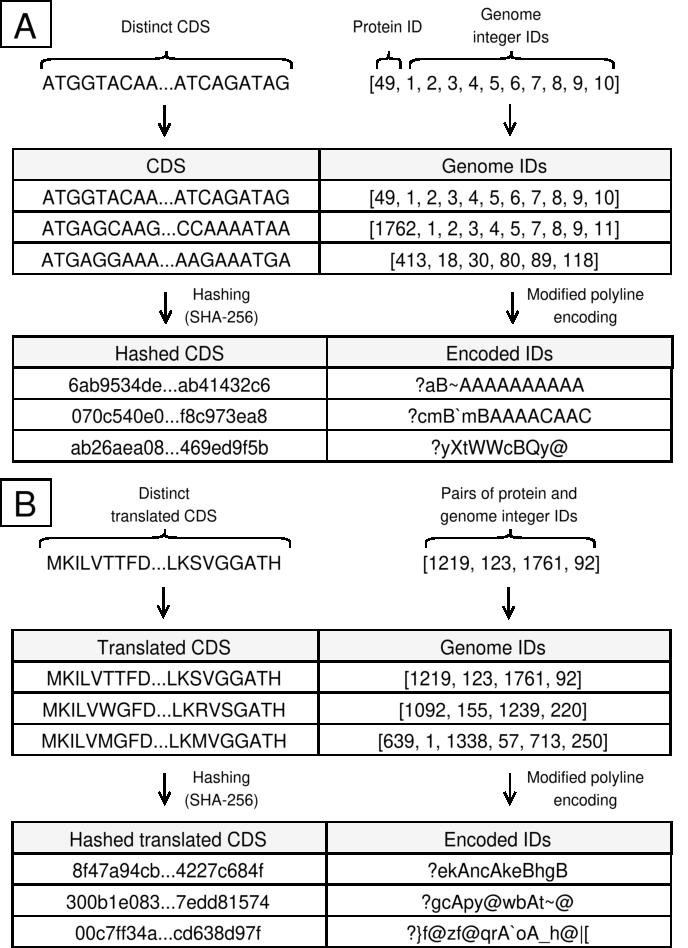
\includegraphics[angle=0,width=0.9\textwidth]{figures/chapter 2/FigureS7.pdf}
    \caption{Sequence hashing and modified polyline encoding. (A) Each distinct CDS identified in the input genomes is hashed with the SHA-256 algorithm implemented in Python's hashlib library. The hash digest is obtained through the hexdigest method and mapped to the list of integer identifiers for the genomes containing the CDS encoded with modified polyline encoding. (B) After sequence translation and deduplication, each distinct translated CDS is hashed with the SHA-256 algorithm and the hash digest is mapped against lists with pairs of protein and genome identifiers used to identify each distinct CDS coding for the protein encoded with modified polyline encoding. The modified polyline encoding is applied to reduce the memory used to retain the data in-memory during the process, drastically reducing peak memory usage when processing large datasets. The Python dictionaries created to map the hashes to the lists of identifiers allow quick identification and classification of exact and inexact matches.}
    \label{fig:chap2_figureS7}
\end{figure*}

\newpage
\begin{figure*}[h!]
    \centering
    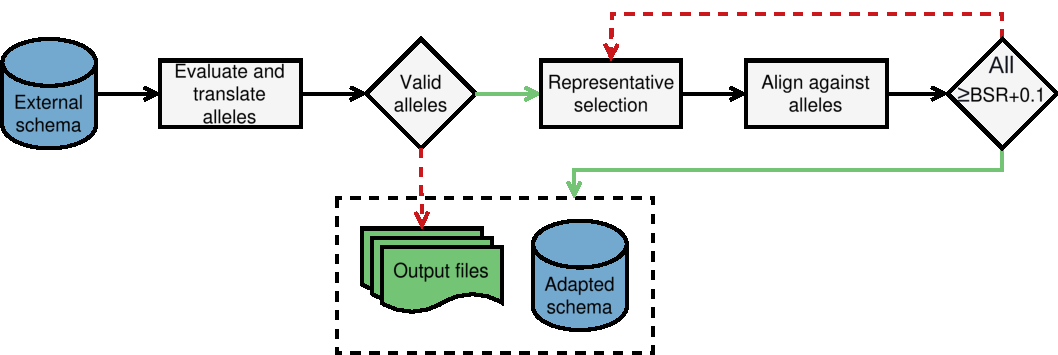
\includegraphics[angle=0,width=\textwidth]{figures/chapter 2/FigureS8.pdf}
    \caption{Diagram of the PrepExternalSchema module. The PrepExternalSchema module adapts schemas created with other wg/cgMLST tools or available on external platforms for usage with chewBBACA 3. The process starts by validating and translating the alleles in the external schema. Incomplete (i.e. size not multiple of 3) and invalid (i.e. missing the start or stop codons, or containing in-frame stop codons) alleles, alleles containing ambiguous bases or smaller than the specified minimum length value, are excluded. For each locus that has valid alleles, the process selects the largest or one of the largest alleles as the first representative allele. The representative is aligned against the locus' alleles with BLASTp to compute the BSR for each alignment. If all the BSR values are above the specified BSR plus 0.1, it is considered that the representative allele can adequately capture the diversity of the locus. Otherwise, new representative alleles are selected from those with a BSR above the specified BSR but below that value plus 0.1 to align against the locus' alleles and determine if the set of representative alleles selected captures the locus diversity adequately. Representative selection is repeated until all locus' alleles have a BSR above the specified value plus 0.1 with at least one of the selected representative alleles. The valid and selected representative alleles are written to FASTA files to create a schema compatible with chewBBACA. The list of invalid alleles, the list of loci excluded from the adapted schema due to having no valid alleles, and the number of total alleles and representative alleles per locus in the adapted schema are stored in output files. The green document icons represent output files. Grey rectangle icons represent analysis steps. Diamond icons represent conditional statements, with green arrows used when the condition is met and red dashed arrows otherwise. The blue cylinder icons represent schemas.}
    \label{fig:chap2_figureS8}
\end{figure*}

\newpage
\begin{figure*}[h!]
    \centering
    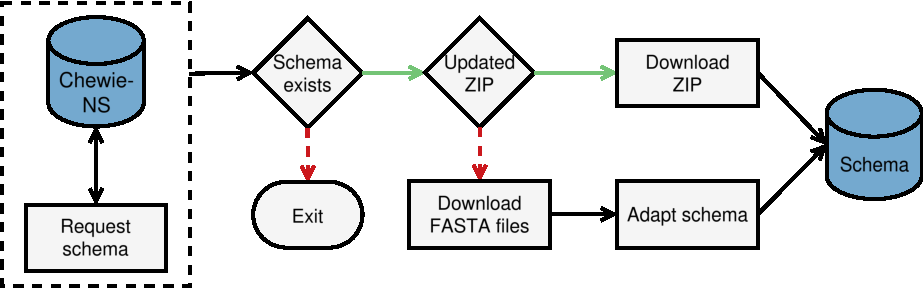
\includegraphics[angle=0,width=\textwidth]{figures/chapter 2/FigureS9.pdf}
    \caption{Diagram of the DownloadSchema module. The DownloadSchema module imports schemas from Chewie-NS. The process starts by sending a request with species and schema identifiers to Chewie-NS. If the schema exists, the process checks for a compressed and up-to-date version of the schema to download. If the compressed schema in Chewie-NS is for the latest version of the schema, the compressed schema is downloaded and uncompressed to get a ready-to-use schema. Otherwise, the process will send requests to retrieve the FASTA files with the alleles for all loci and determine the representative alleles with the PrepExternalSchema module to create the schema locally. Grey rectangle icons represent analysis steps. Diamond icons represent conditional statements, with green arrows used when the condition is met and red dashed arrows otherwise. The blue cylinder icons represent schemas.}
    \label{fig:chap2_figureS9}
\end{figure*}

\newpage
\begin{figure*}[h!]
    \centering
    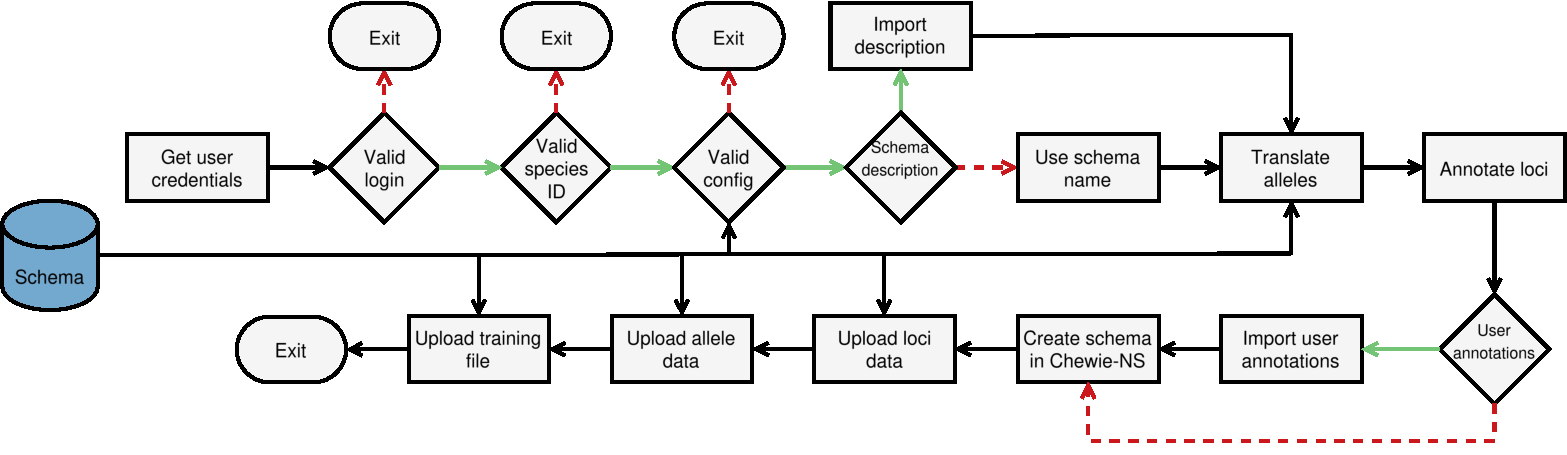
\includegraphics[angle=0,width=\textwidth]{figures/chapter 2/FigureS10.pdf}
    \caption{Diagram of the LoadSchema module. The LoadSchema module uploads local schemas to Chewie-NS. The process starts by requesting the user credentials to ensure that the user has contributor privileges. Only contributors are allowed to upload schemas to Chewie-NS. If the user is a contributor, the process checks if the species identifier provided by the user is valid and if the species is listed in Chewie-NS. After this step, the process reads the schema’s configuration file to validate the schema parameter values and ensure that there is only a single value associated with each parameter. The initial validation steps are followed by the upload of the schema data to Chewie-NS. The process reads the schema description, if the user provided one, or uses the schema name as description. The alleles are translated and annotation terms for the loci are obtained through UniProt’s SPARQL endpoint. If the user provides custom loci annotations, the process reads the file provided by the user and adds the custom annotations to the loci annotation data to send to Chewie-NS. After retrieving loci annotations, the process creates the schema in Chewie-NS by sending the schema’s parameter values and the list of file hashes to validate schema files uploaded in subsequent steps. The loci are created and linked to the newly created schema by sending the loci identifiers and annotations to Chewie-NS. The loci FASTA files are compressed and uploaded to Chewie-NS to add the allele sequences to the database and link them to the corresponding loci. The last step in the process uploads the training file in the local schema and associates it to the newly created schema in Chewie-NS. After process completion, Chewie-NS will process the data that was sent to make the schema data and statistics available through the website and the API. Grey rectangle icons represent analysis steps. Diamond icons represent conditional statements, with green arrows used when the condition is met and red dashed arrows otherwise. The blue cylinder icon represents a schema.}
    \label{fig:chap2_figureS10}
\end{figure*}

\newpage
\begin{figure*}[h!]
    \centering
    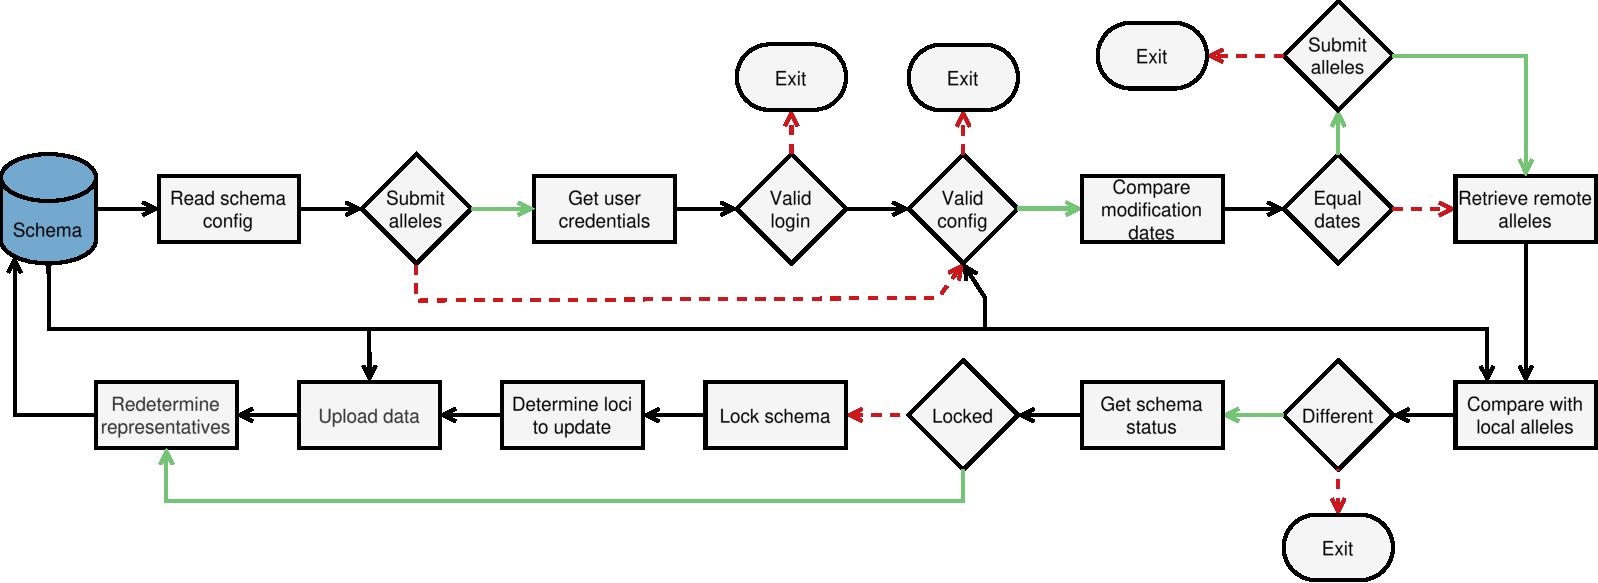
\includegraphics[angle=0,width=\textwidth]{figures/chapter 2/FigureS11.pdf}
    \caption{Diagram of the SyncSchema module. The SyncSchema module retrieves new alleles added to remote schemas in Chewie-NS and submits new alleles added to local schemas to update the remote schemas in Chewie-NS. The process starts by reading the schema’s configuration file to get the schema’s parameter values and ensure the values match the ones listed in Chewie-NS. If the user wants to submit new alleles identified locally (--submit), the process will ask for the user credentials to verify if the user has contributor privileges. Before retrieving or uploading new alleles, the process verifies if the last modification date of the local and remote schemas match. If the dates match and the user does not want to submit new local alleles, the process exits. If the dates do not match or the user wants to submit new local alleles, the process retrieves new alleles added to the remote schema since the last modification date and compares them with the alleles in the local schema. If any alleles are exclusive to the local or remote schema, the process creates updated FASTA files with all the alleles and locks the remote schema to ensure that only the current user can modify the remote schema. The process creates files with the data for the new local alleles and sends them to Chewie-NS, waiting for Chewie-NS to insert the new alleles into the database. After allele insertion in Chewie-NS, the process adapts the updated FASTA files with the PrepExternalSchema module to update the local schema and ensure that the local and remote allele identifiers match. If the schema was already locked by another user, the process will skip data upload to Chewie-NS and will update the local schema with new alleles retrieved from Chewie-NS. Grey rectangle icons represent analysis steps. Diamond icons represent conditional statements, with green arrows used when the condition is met and red dashed arrows otherwise. The blue cylinder icon represents a schema.}
    \label{fig:chap2_figureS11}
\end{figure*}

\newpage
\begin{figure*}[h!]
    \centering
    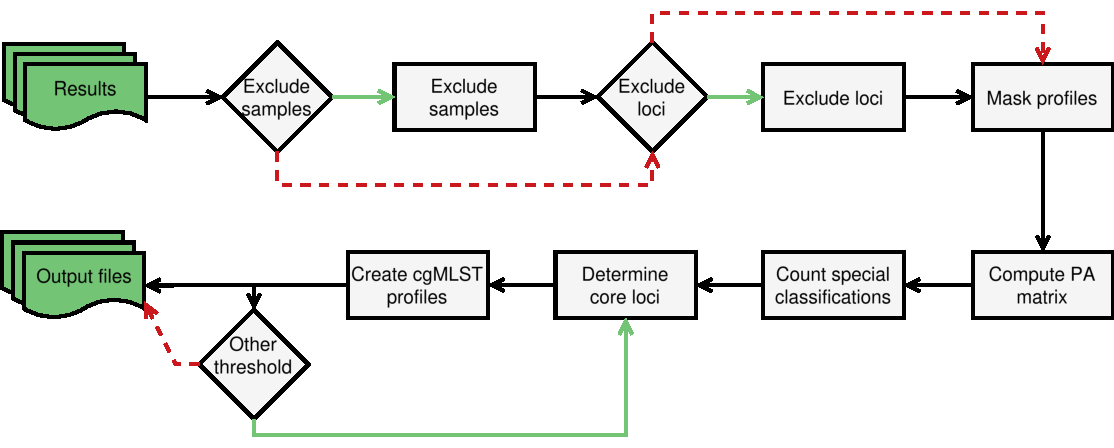
\includegraphics[angle=0,width=\textwidth]{figures/chapter 2/FigureS12.pdf}
    \caption{Diagram of the ExtractCgMLST module. The ExtractCgMLST module determines the set of core loci based on the allelic profiles determined by the AlleleCall module. The process starts by excluding loci and samples from the analysis based on lists of loci and samples provided by the user. This allows users to filter out low-quality samples and problematic loci that would affect the determination of the core genome. The filtered allelic profiles are masked to remove the INF- prefixes from newly inferred alleles and substitute special classifications by 0. The masked profiles are used to compute a loci presence-absence matrix and count the number of special classifications per sample. The presence-absence matrix is also used to determine the set of core loci based on the default loci presence thresholds of 0.9, 0.95 and 1, or based on threshold values specified by the user. The process creates output files with the list of loci and allelic profiles per threshold and creates an HTML file with a scatter plot representing the core genome size variation for each threshold. The green document icons represent input and output files. Grey rectangle icons represent analysis steps. Diamond icons represent conditional statements, with green arrows used when the condition is met and red dashed arrows otherwise.}
    \label{fig:chap2_figureS12}
\end{figure*}

\newpage
\begin{figure*}[h!]
    \centering
    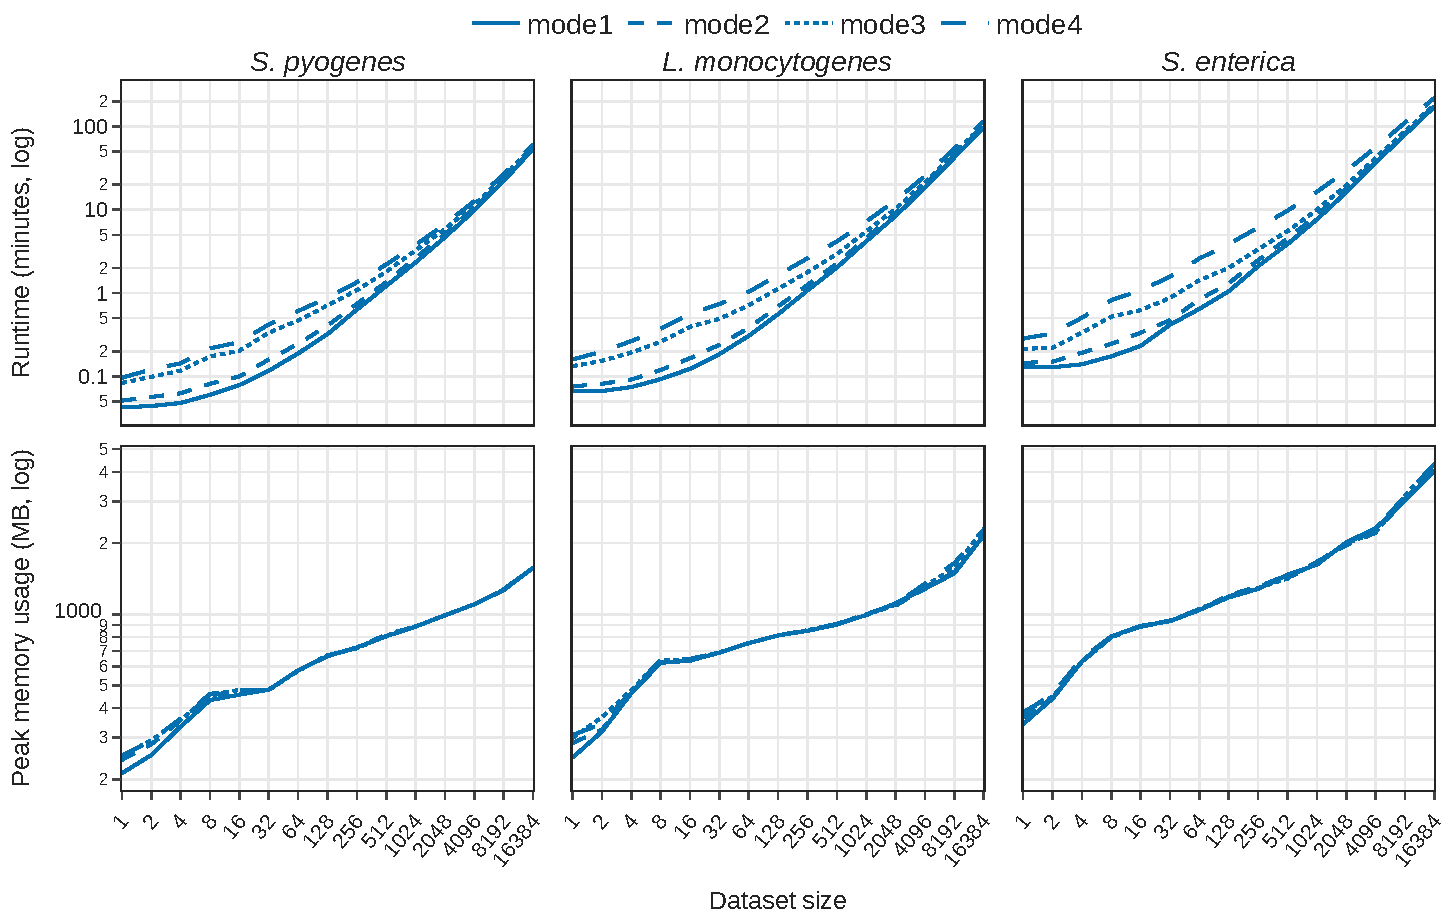
\includegraphics[angle=0,width=\textwidth]{figures/chapter 2/FigureS13.pdf}
    \caption{Runtime and peak memory usage for the four execution modes available in chewBBACA 3. Runtime and peak memory usage were measured for the allele calling of datasets with 1 to 16384 strains for three bacterial species: Streptococcus pyogenes, Listeria monocytogenes, and Salmonella enterica. The benchmark was performed with five replicates per dataset size, except for the complete dataset (n=16,384 genomes). The values shown are the mean of the replicate values for each dataset. Runtime was measured as the elapsed real time in minutes (logarithmic scale). Peak memory usage was measured as the maximum resident set size in MB (logarithmic scale).}
    \label{fig:chap2_figureS13}
\end{figure*}

\newpage
\begin{figure*}[h!]
    \centering
    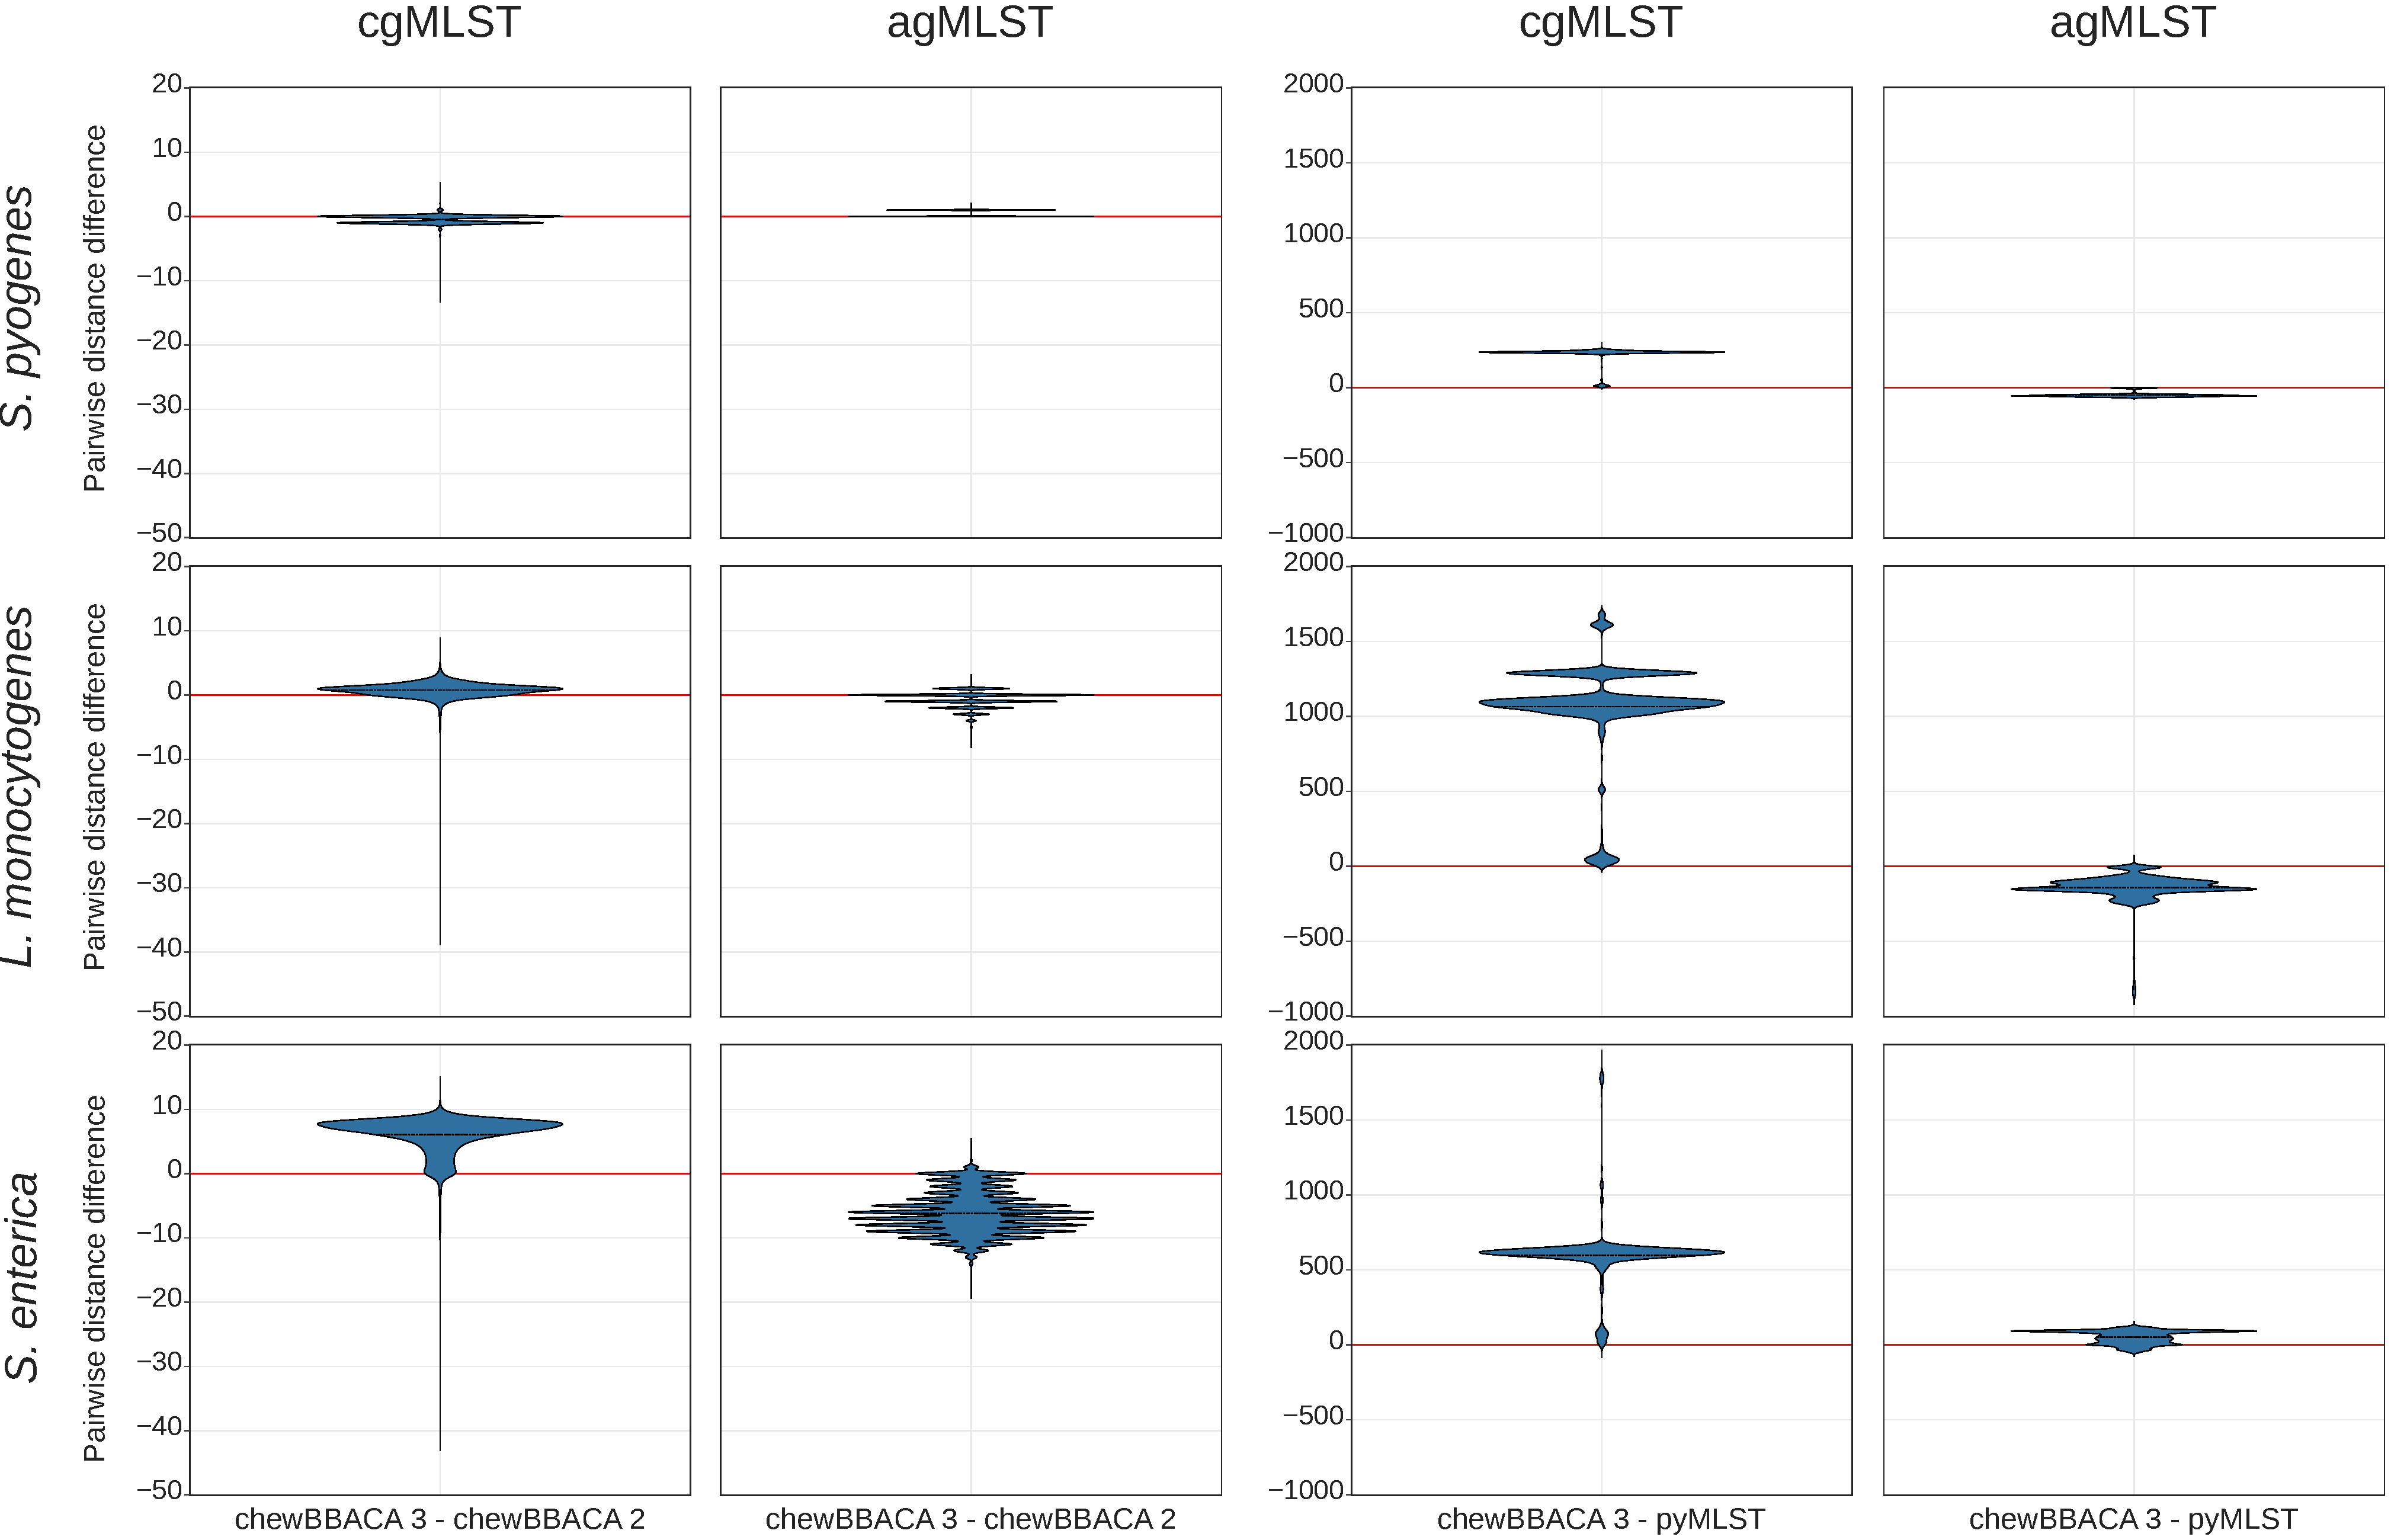
\includegraphics[angle=0,width=\textwidth]{figures/chapter 2/FigureS14.pdf}
    \caption{Pairwise allelic distances differences. The pairwise distances differences at the core-genome (cgMLST) and accessory-genome (agMLST) levels were computed by subtracting the allelic distance matrices computed based on chewBBACA 2's and pyMLST's results from the allelic distance matrices computed from chewBBACA 3's results for the complete datasets (n=16,384 genomes). A positive value represents a greater difference with chewBBACA 3 and a negative value a smaller difference with chewBBACA 3 than with the comparator. The zero line in each plot is highlighted in red.}
    \label{fig:chap2_figureS14}
\end{figure*}

\newpage
\begin{figure*}[h!]
    \centering
    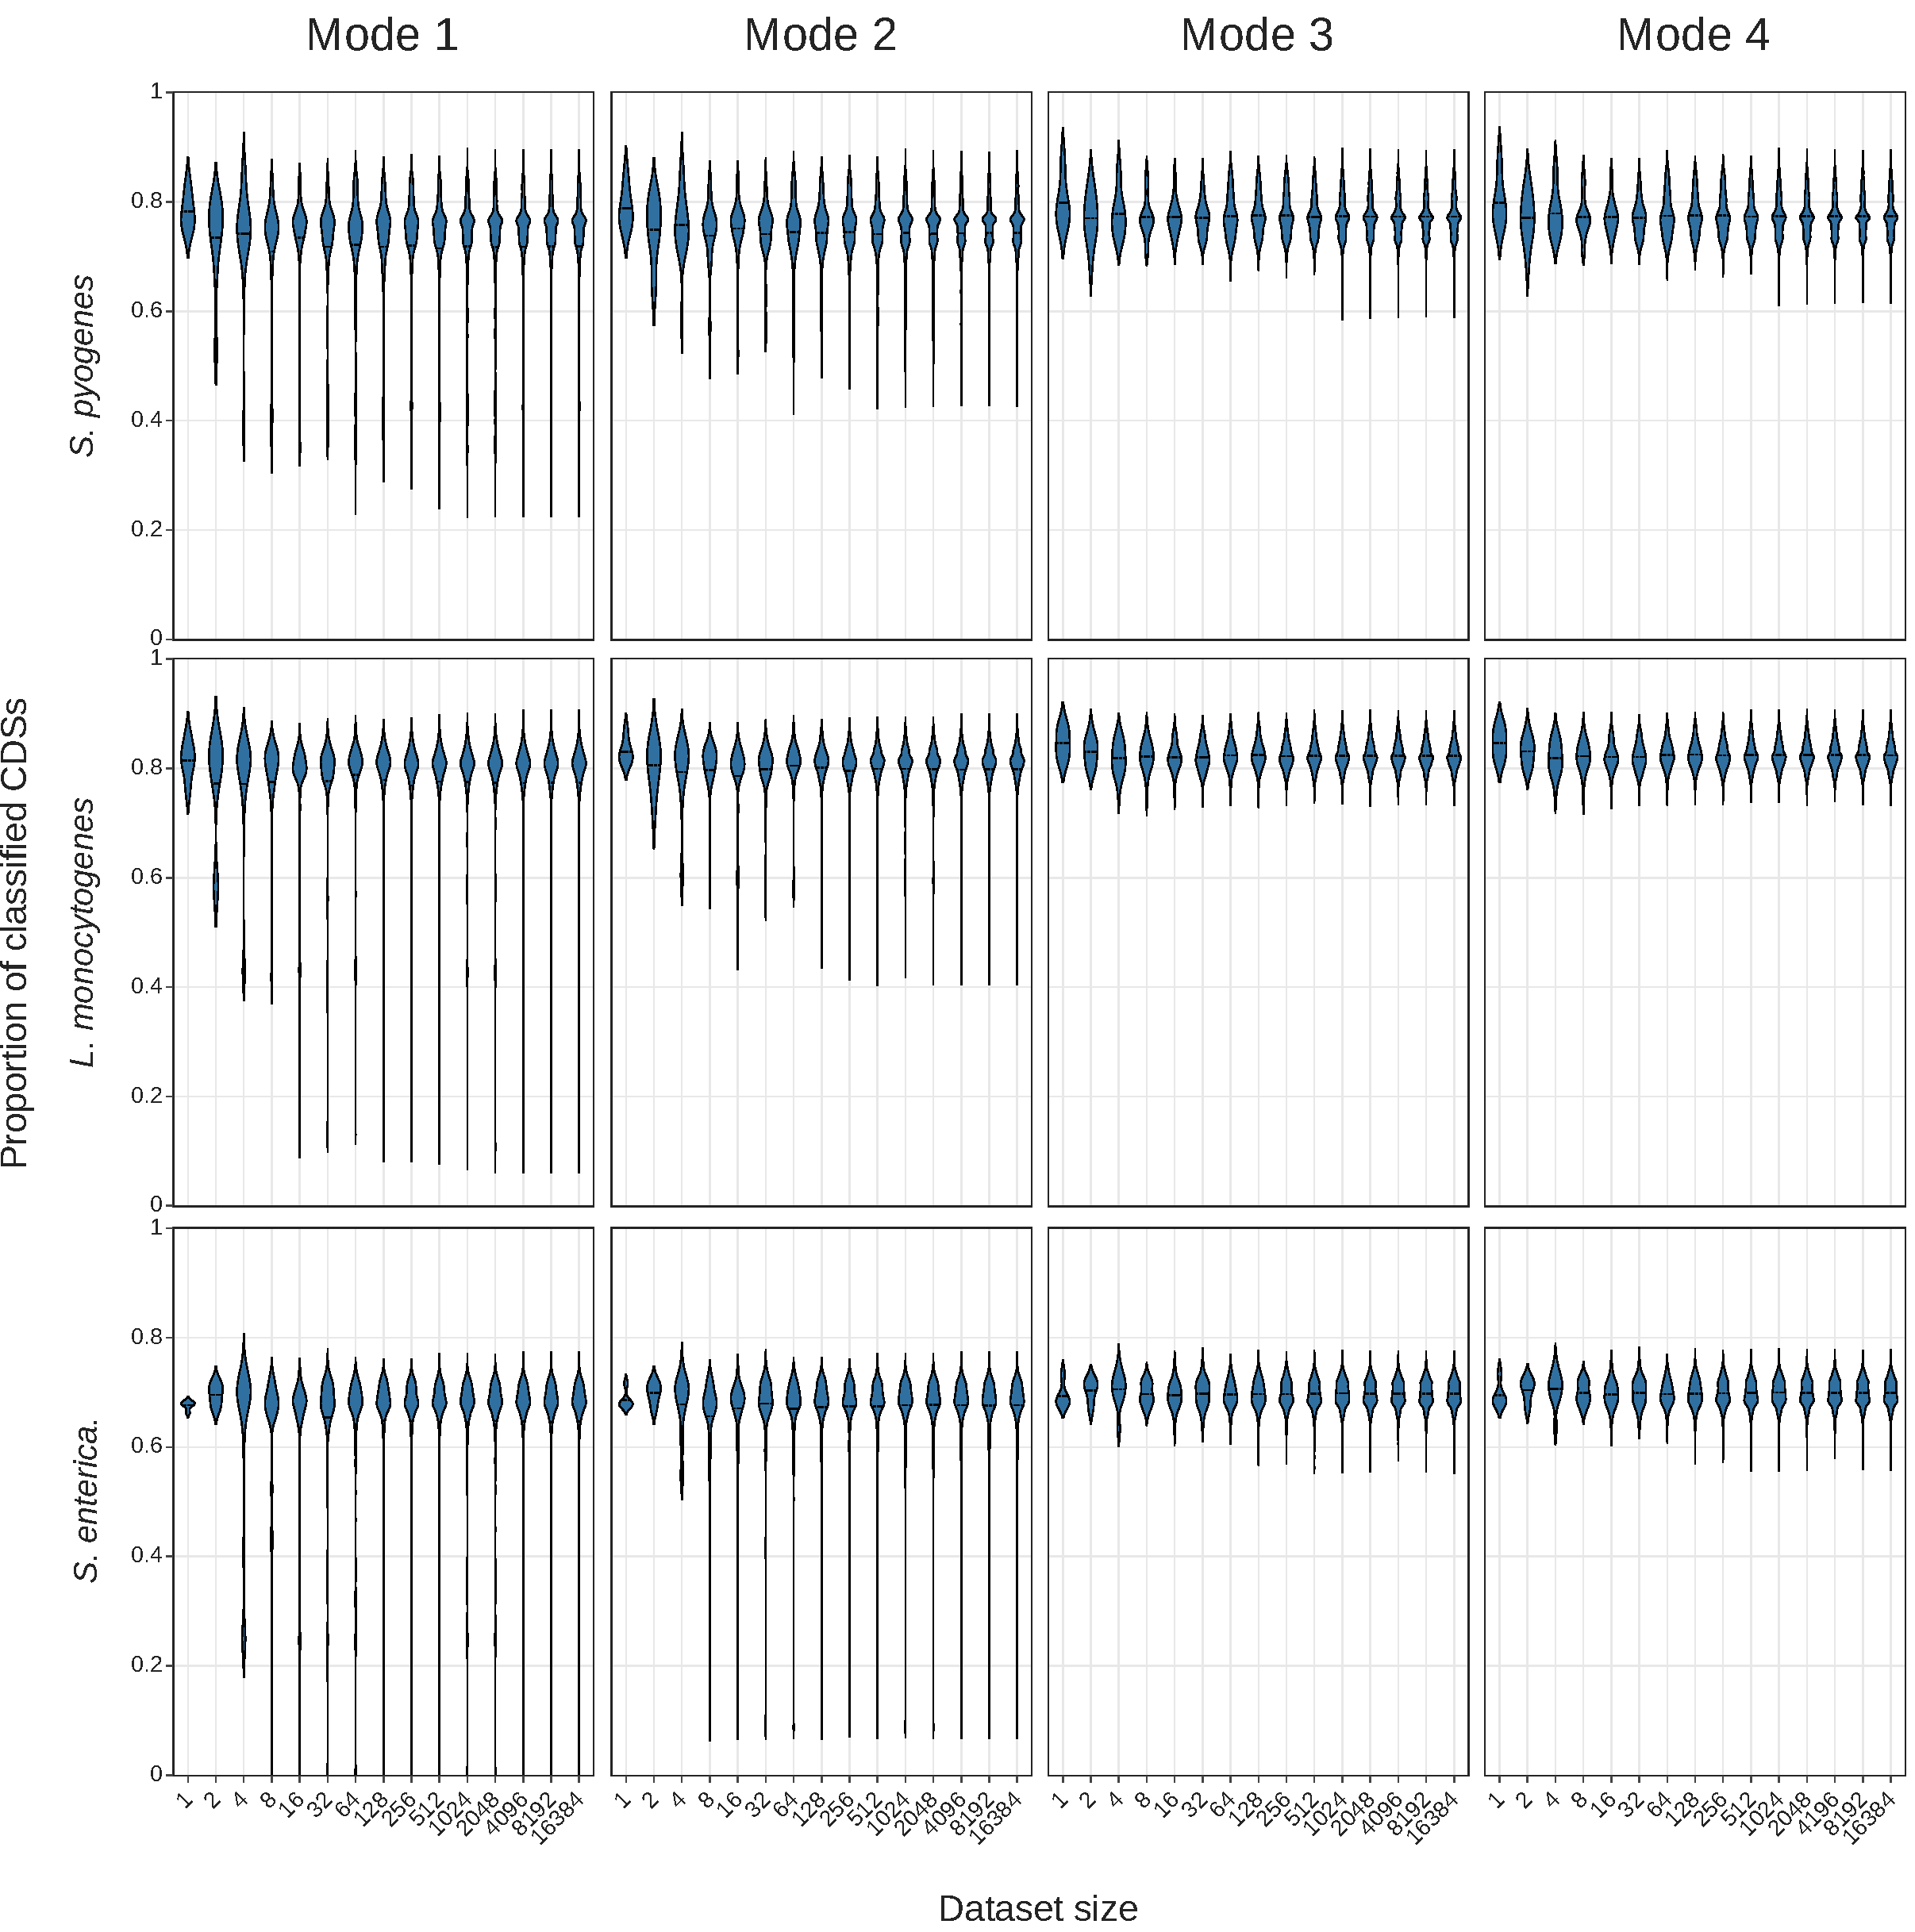
\includegraphics[angle=0,width=\textwidth]{figures/chapter 2/FigureS15.pdf}
    \caption{Proportion of CDSs classified per execution mode for each species’ datasets. The proportion of classified CDSs corresponds to the number of CDSs classified by each execution mode divided by the total number of CDSs predicted for each strain by Pyrodigal. The benchmark was performed with five replicates per dataset size, except for the complete dataset (n=16,384 genomes).}
    \label{fig:chap2_figureS15}
\end{figure*}

\newpage
\begin{figure*}[h!]
    \centering
    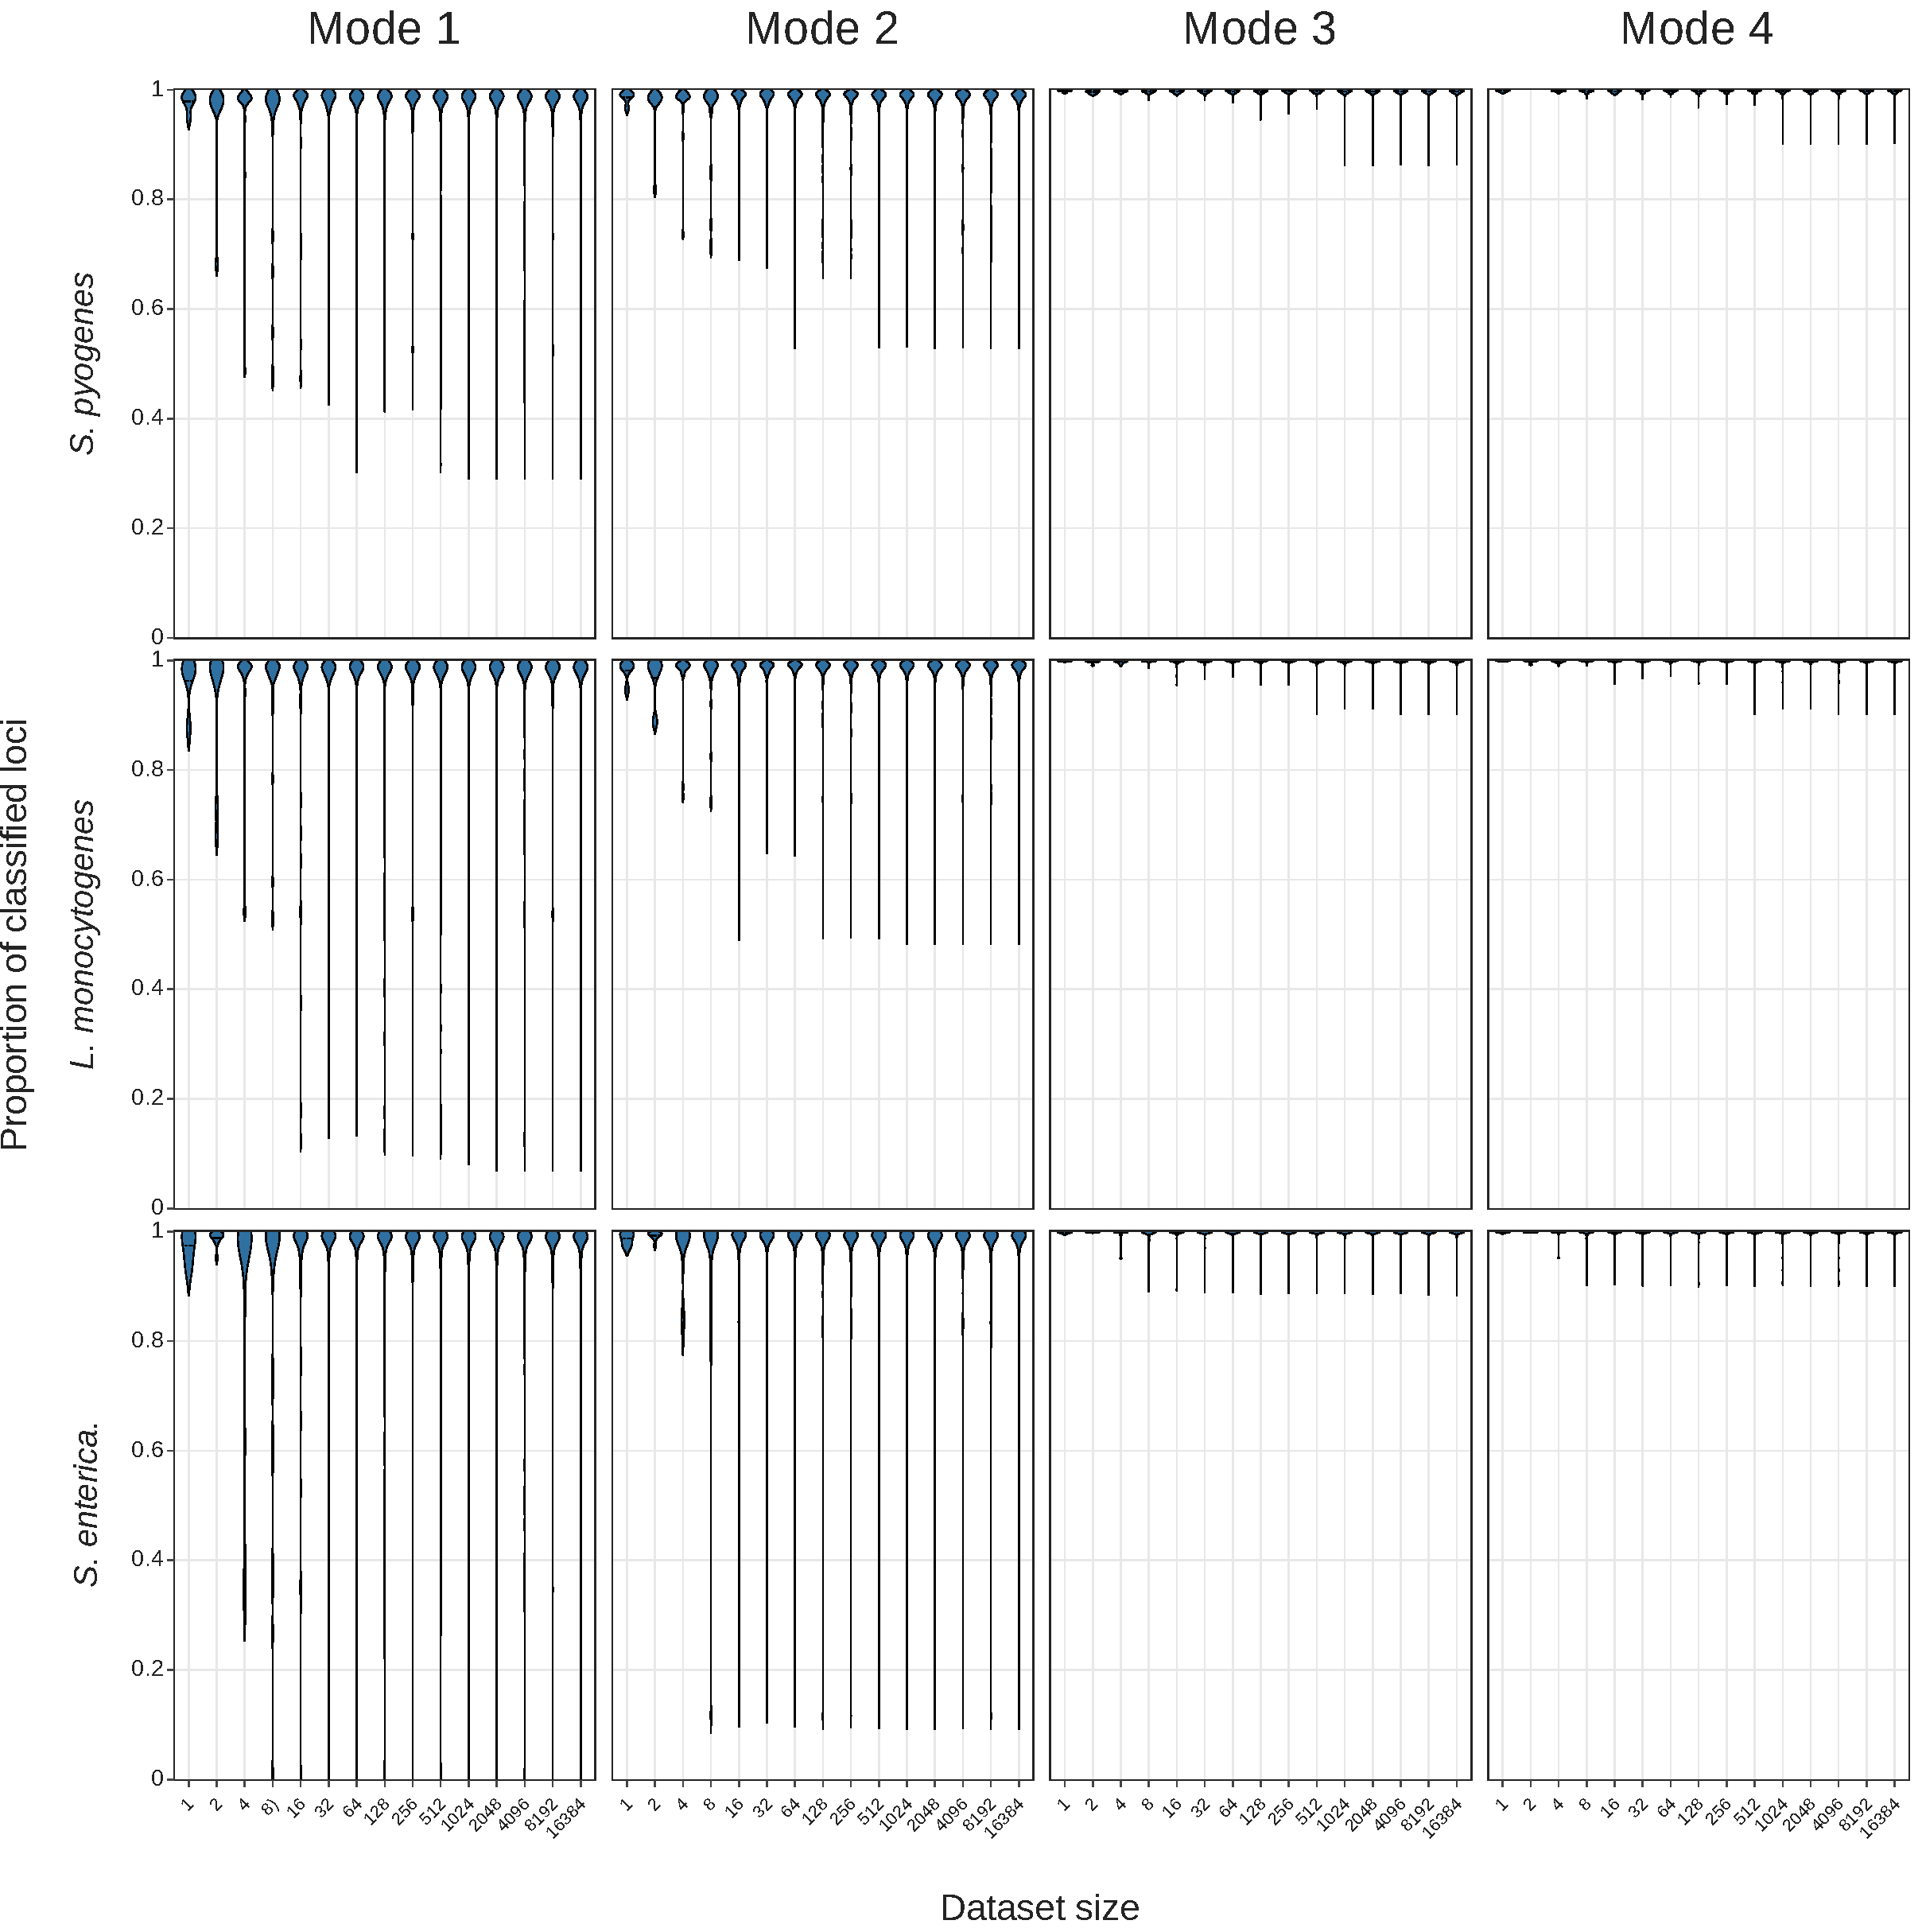
\includegraphics[angle=0,width=\textwidth]{figures/chapter 2/FigureS16.pdf}
    \caption{Proportion of schema loci classified per execution mode for each species’ datasets. The proportion of classified loci corresponds to the number of schema loci identified by each execution mode divided by the total number of schema loci. The benchmark was performed with five replicates per dataset size, except for the complete dataset (n=16,384 genomes).}
    \label{fig:chap2_figureS16}
\end{figure*}

\newpage
\begin{figure*}[h!]
    \centering
    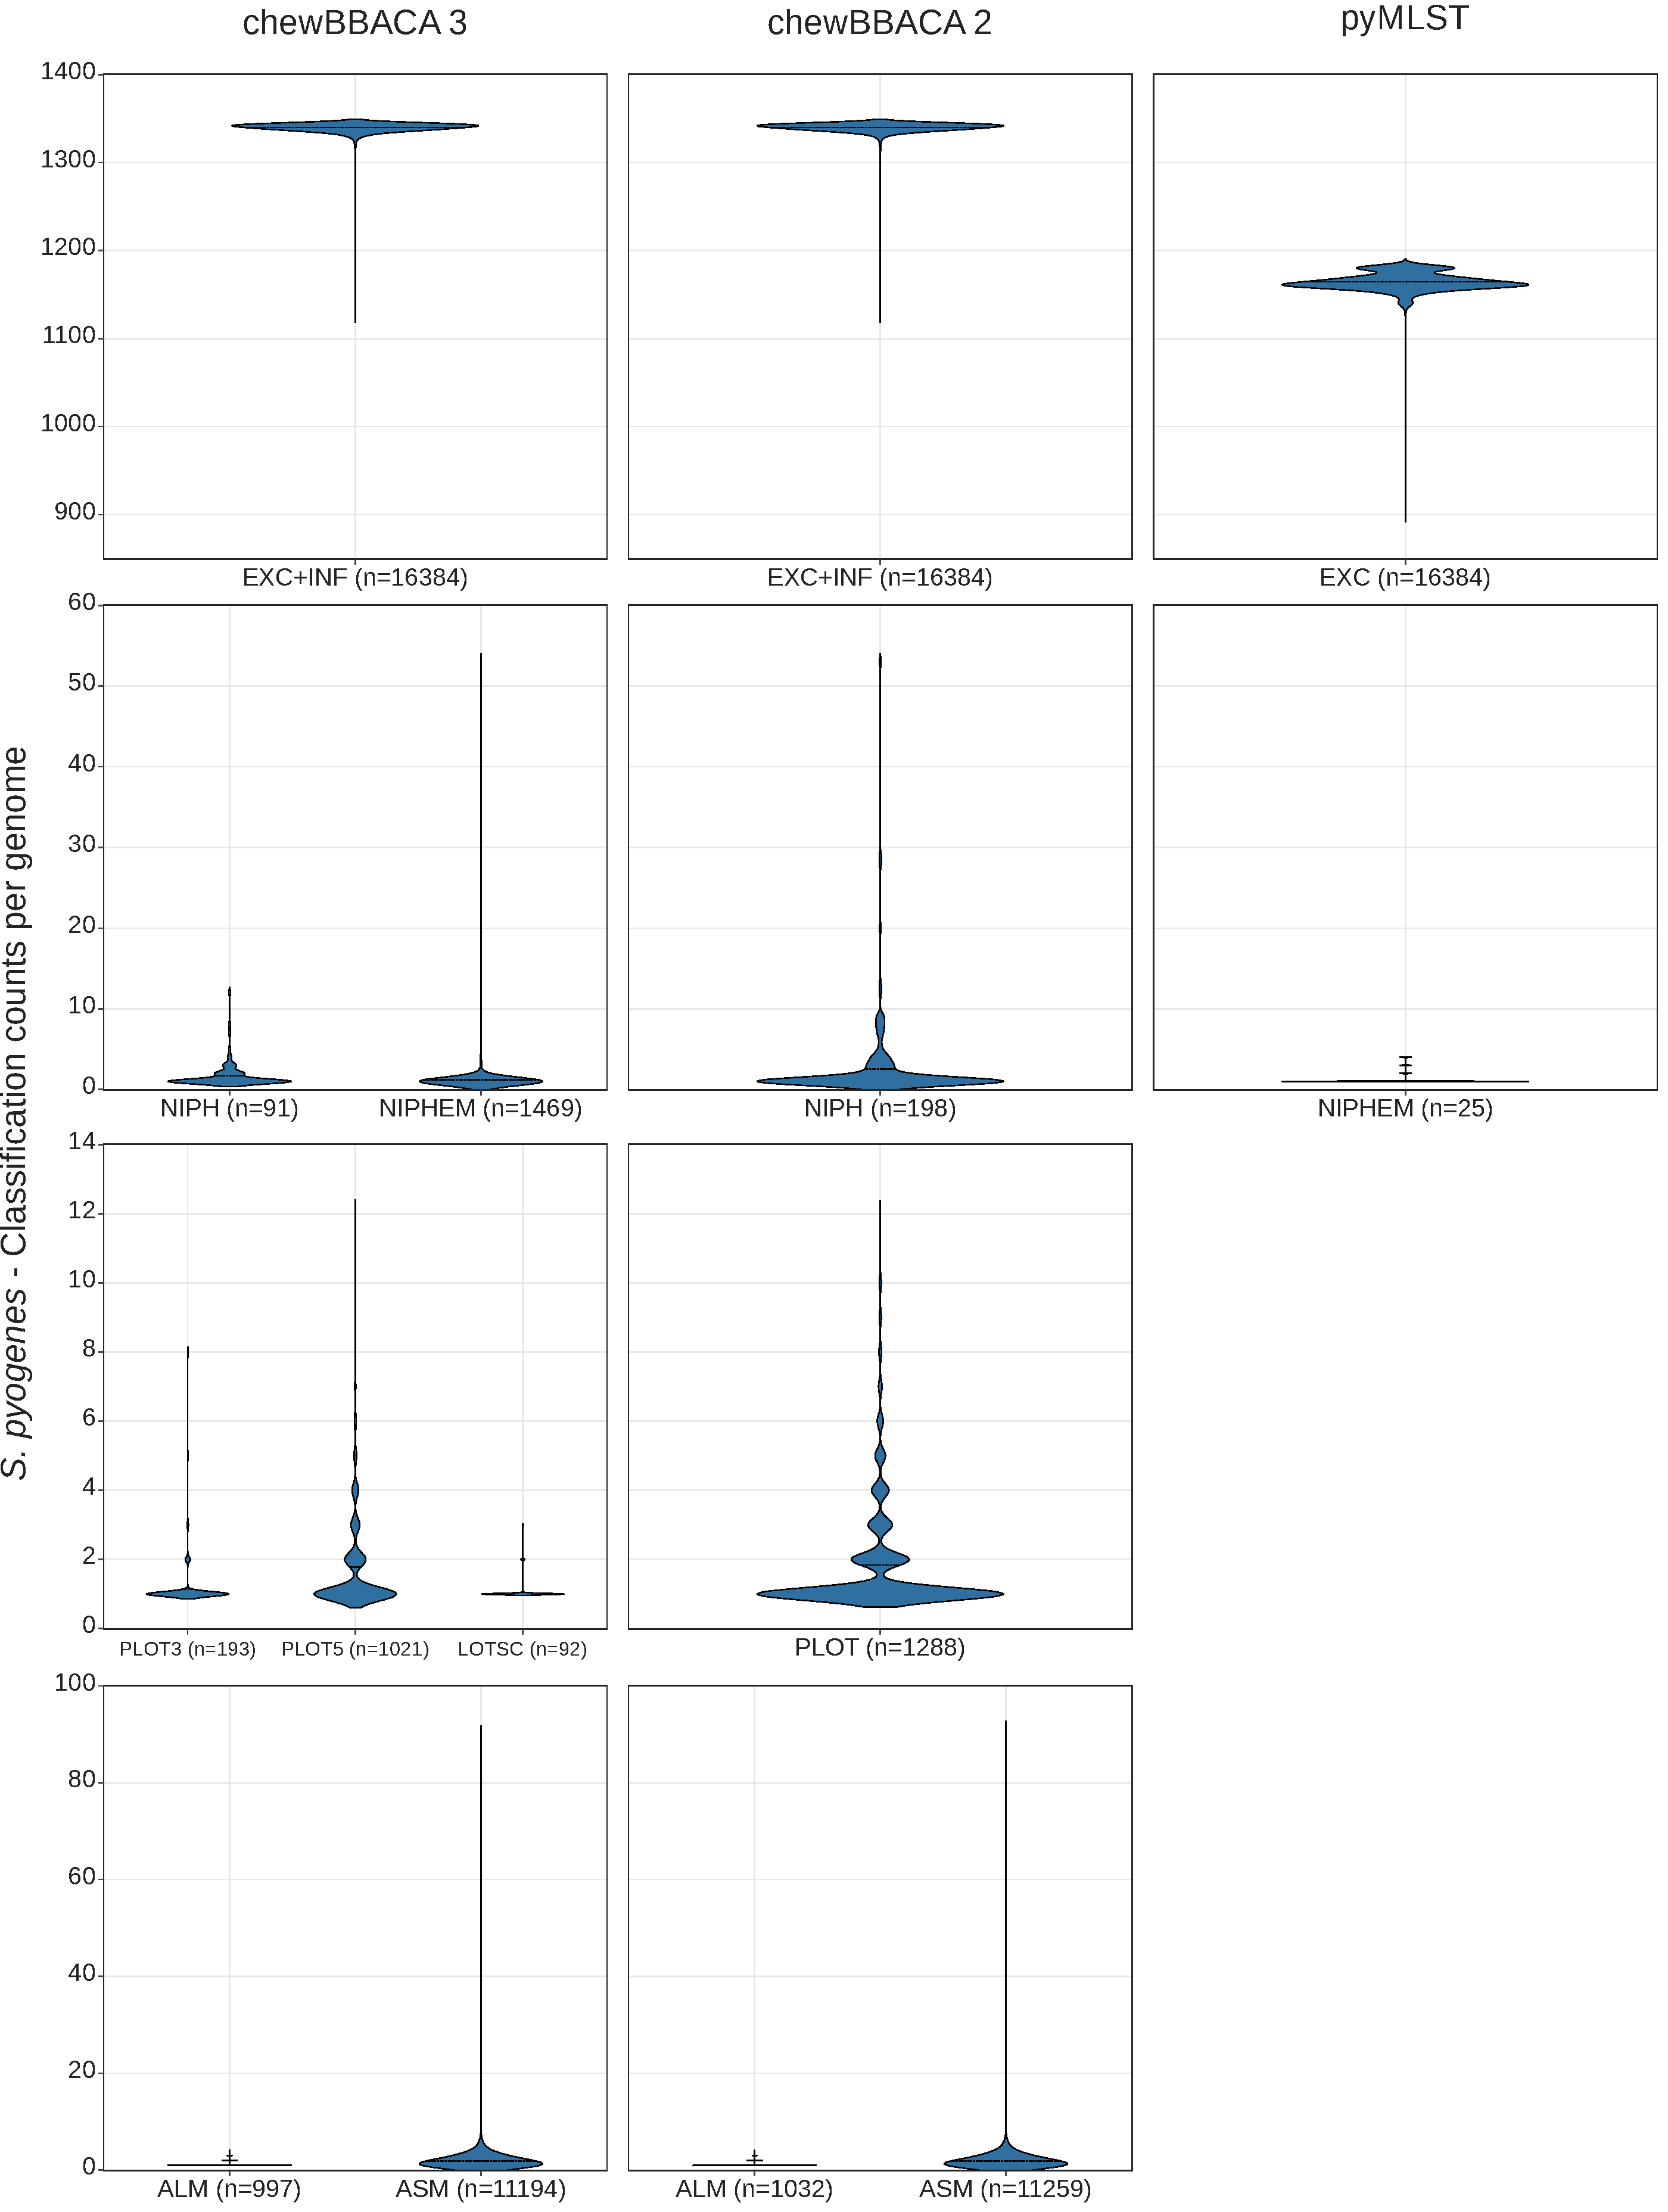
\includegraphics[angle=0,width=\textwidth]{figures/chapter 2/FigureS17.pdf}
    \caption{Classifications counts for the complete dataset (n=16,384 genomes) of S. pyogenes per tool. Each row displays the counts for the special classifications that are equivalent between tools. The x-axis labels show the names of the classifications and the number of genomes with a count above zero inside the parentheses (i.e. genomes with a count of zero for any of the classifications are not included in the plotted values). For pyMLST, the loci with a single matching CDS were converted to EXC and the loci with multiple matches were converted to NIPHEM. The plot is not shown if the tool does not determine a special classification equivalent to the ones displayed in the row.}
    \label{fig:chap2_figureS17}
\end{figure*}

\newpage
\begin{figure*}[h!]
    \centering
    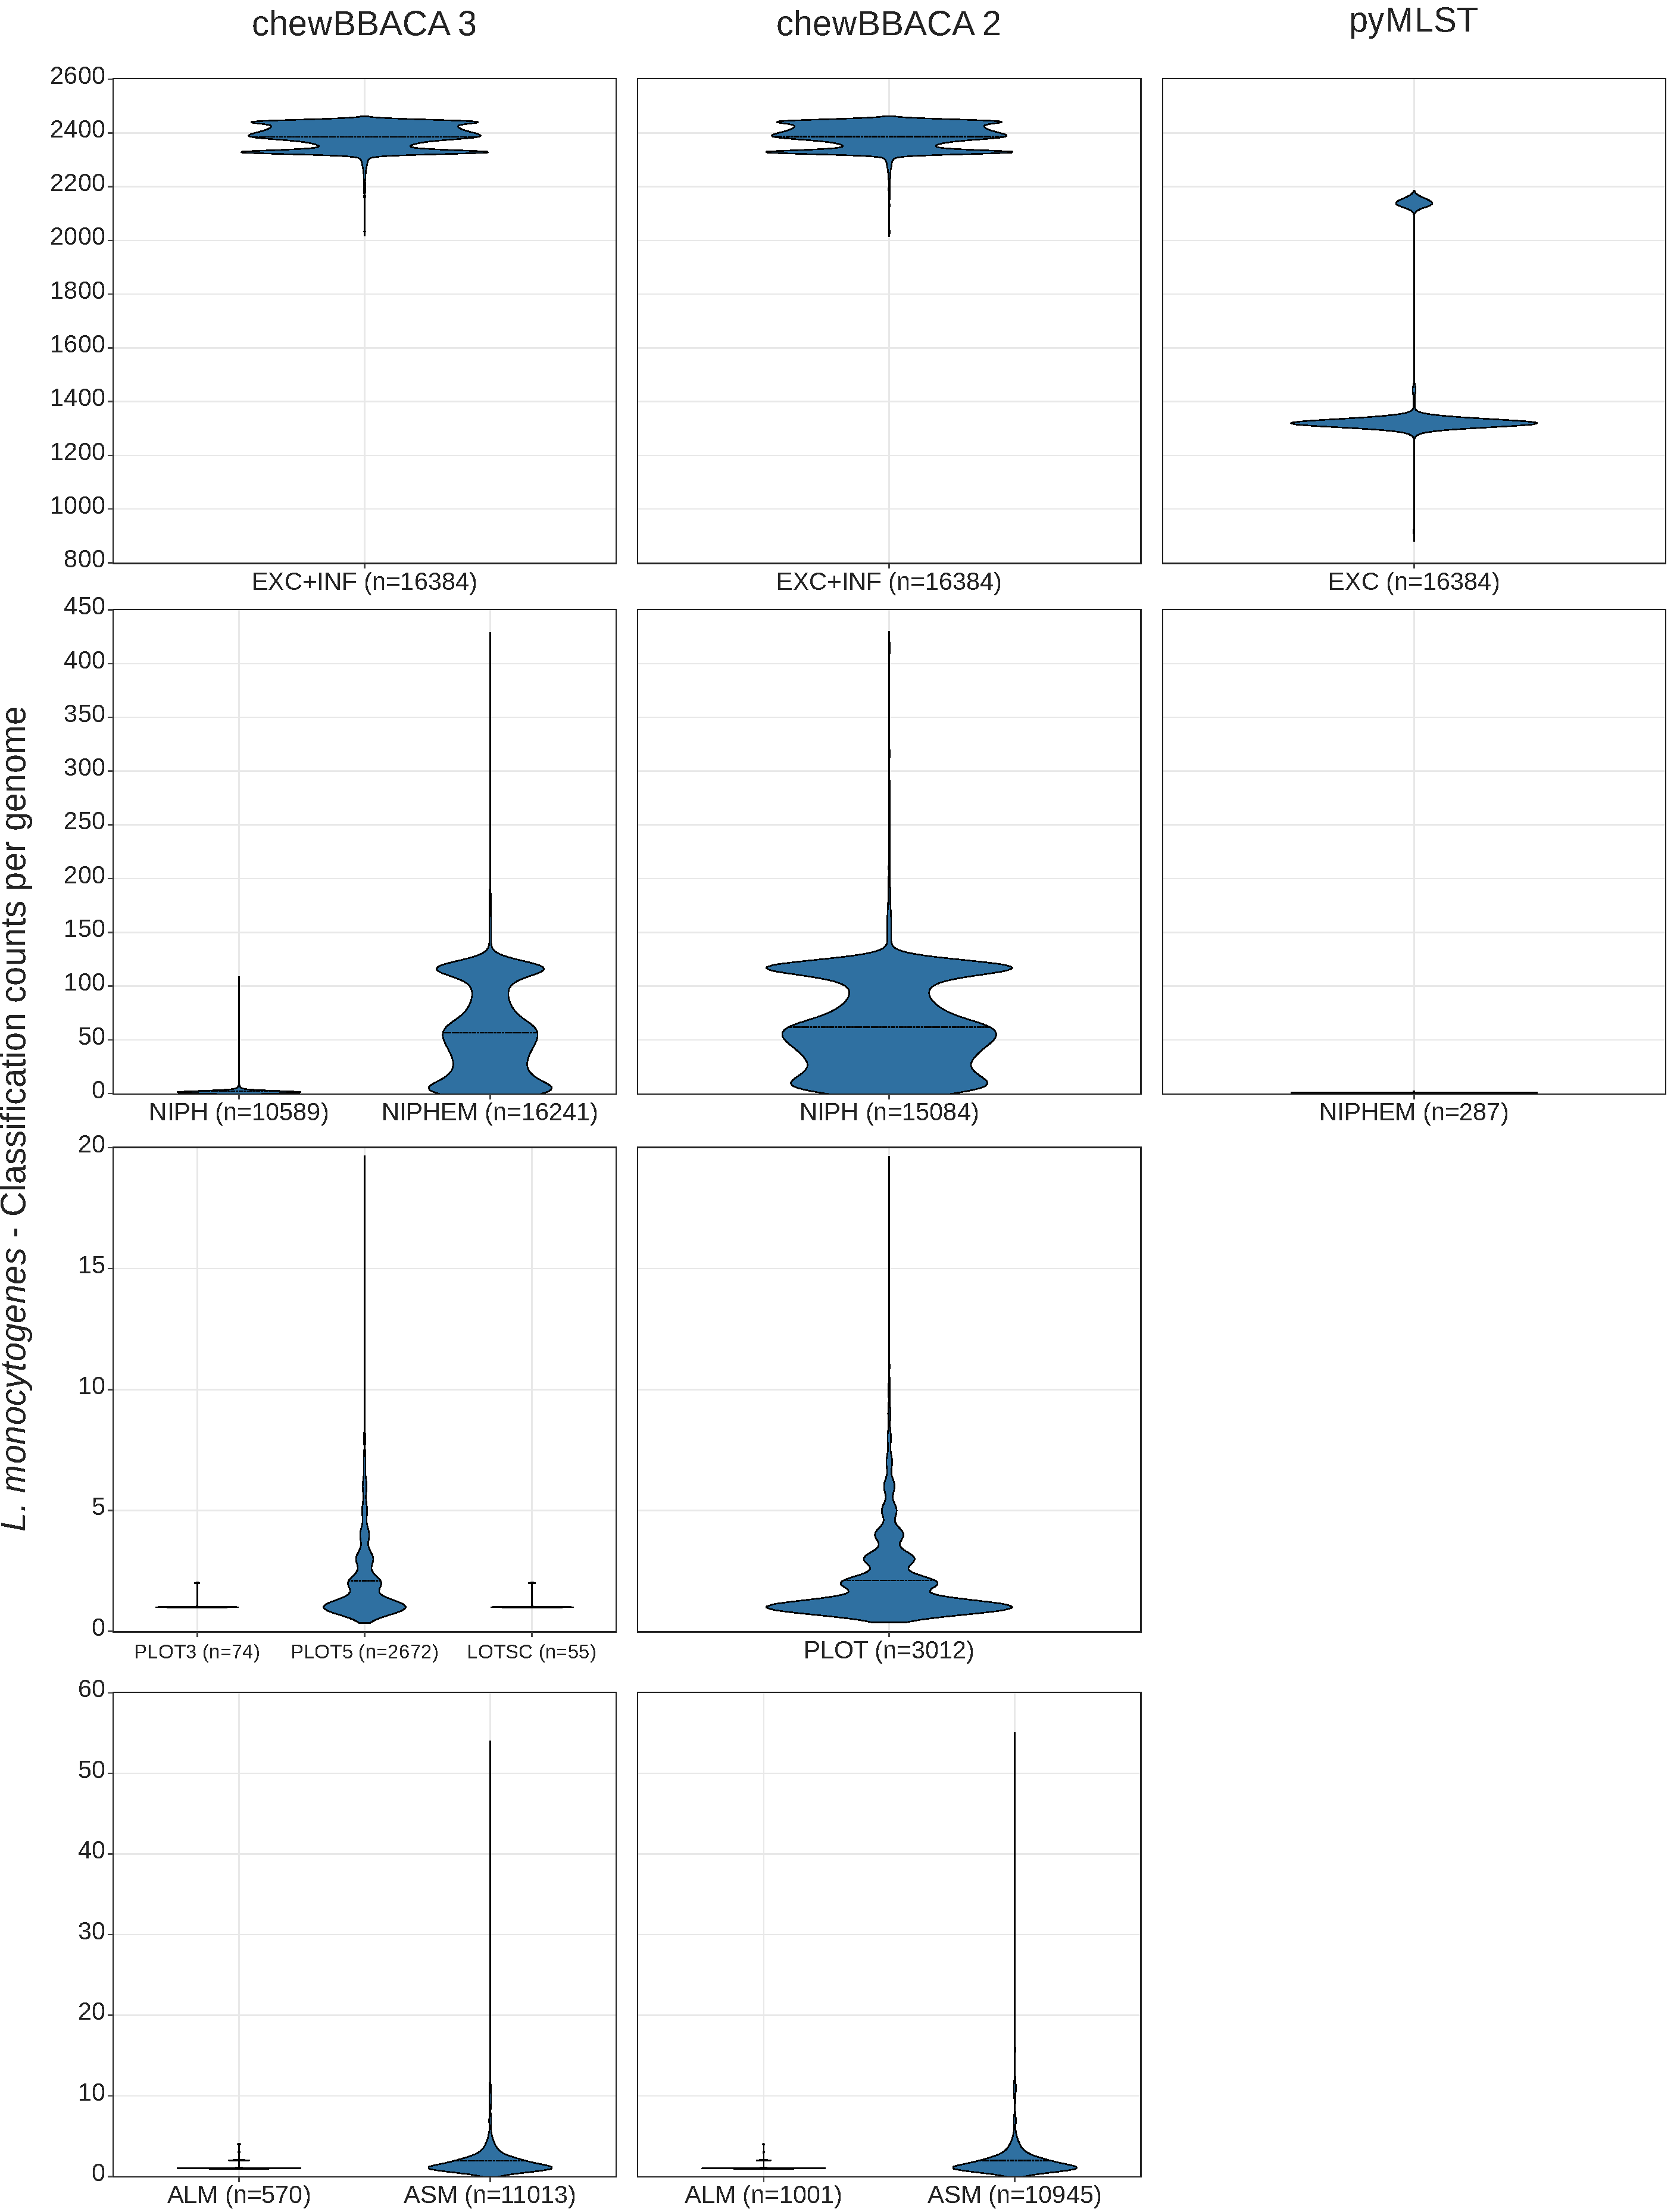
\includegraphics[angle=0,width=\textwidth]{figures/chapter 2/FigureS18.pdf}
    \caption{Classifications counts for the complete dataset (n=16,384 genomes) of L. monocytogenes per tool. Each row displays the counts for the special classifications that are equivalent between tools. The x-axis labels show the names of the classifications and the number of genomes with a count above zero inside the parentheses (i.e. genomes with a count of zero for any of the classifications are not included in the plotted values). For pyMLST, the loci with a single matching CDS were converted to EXC and the loci with multiple matches were converted to NIPHEM. The plot is not shown if the tool does not determine a special classification equivalent to the ones displayed in the row.}
    \label{fig:chap2_figureS18}
\end{figure*}

\newpage
\begin{figure*}[h!]
    \centering
    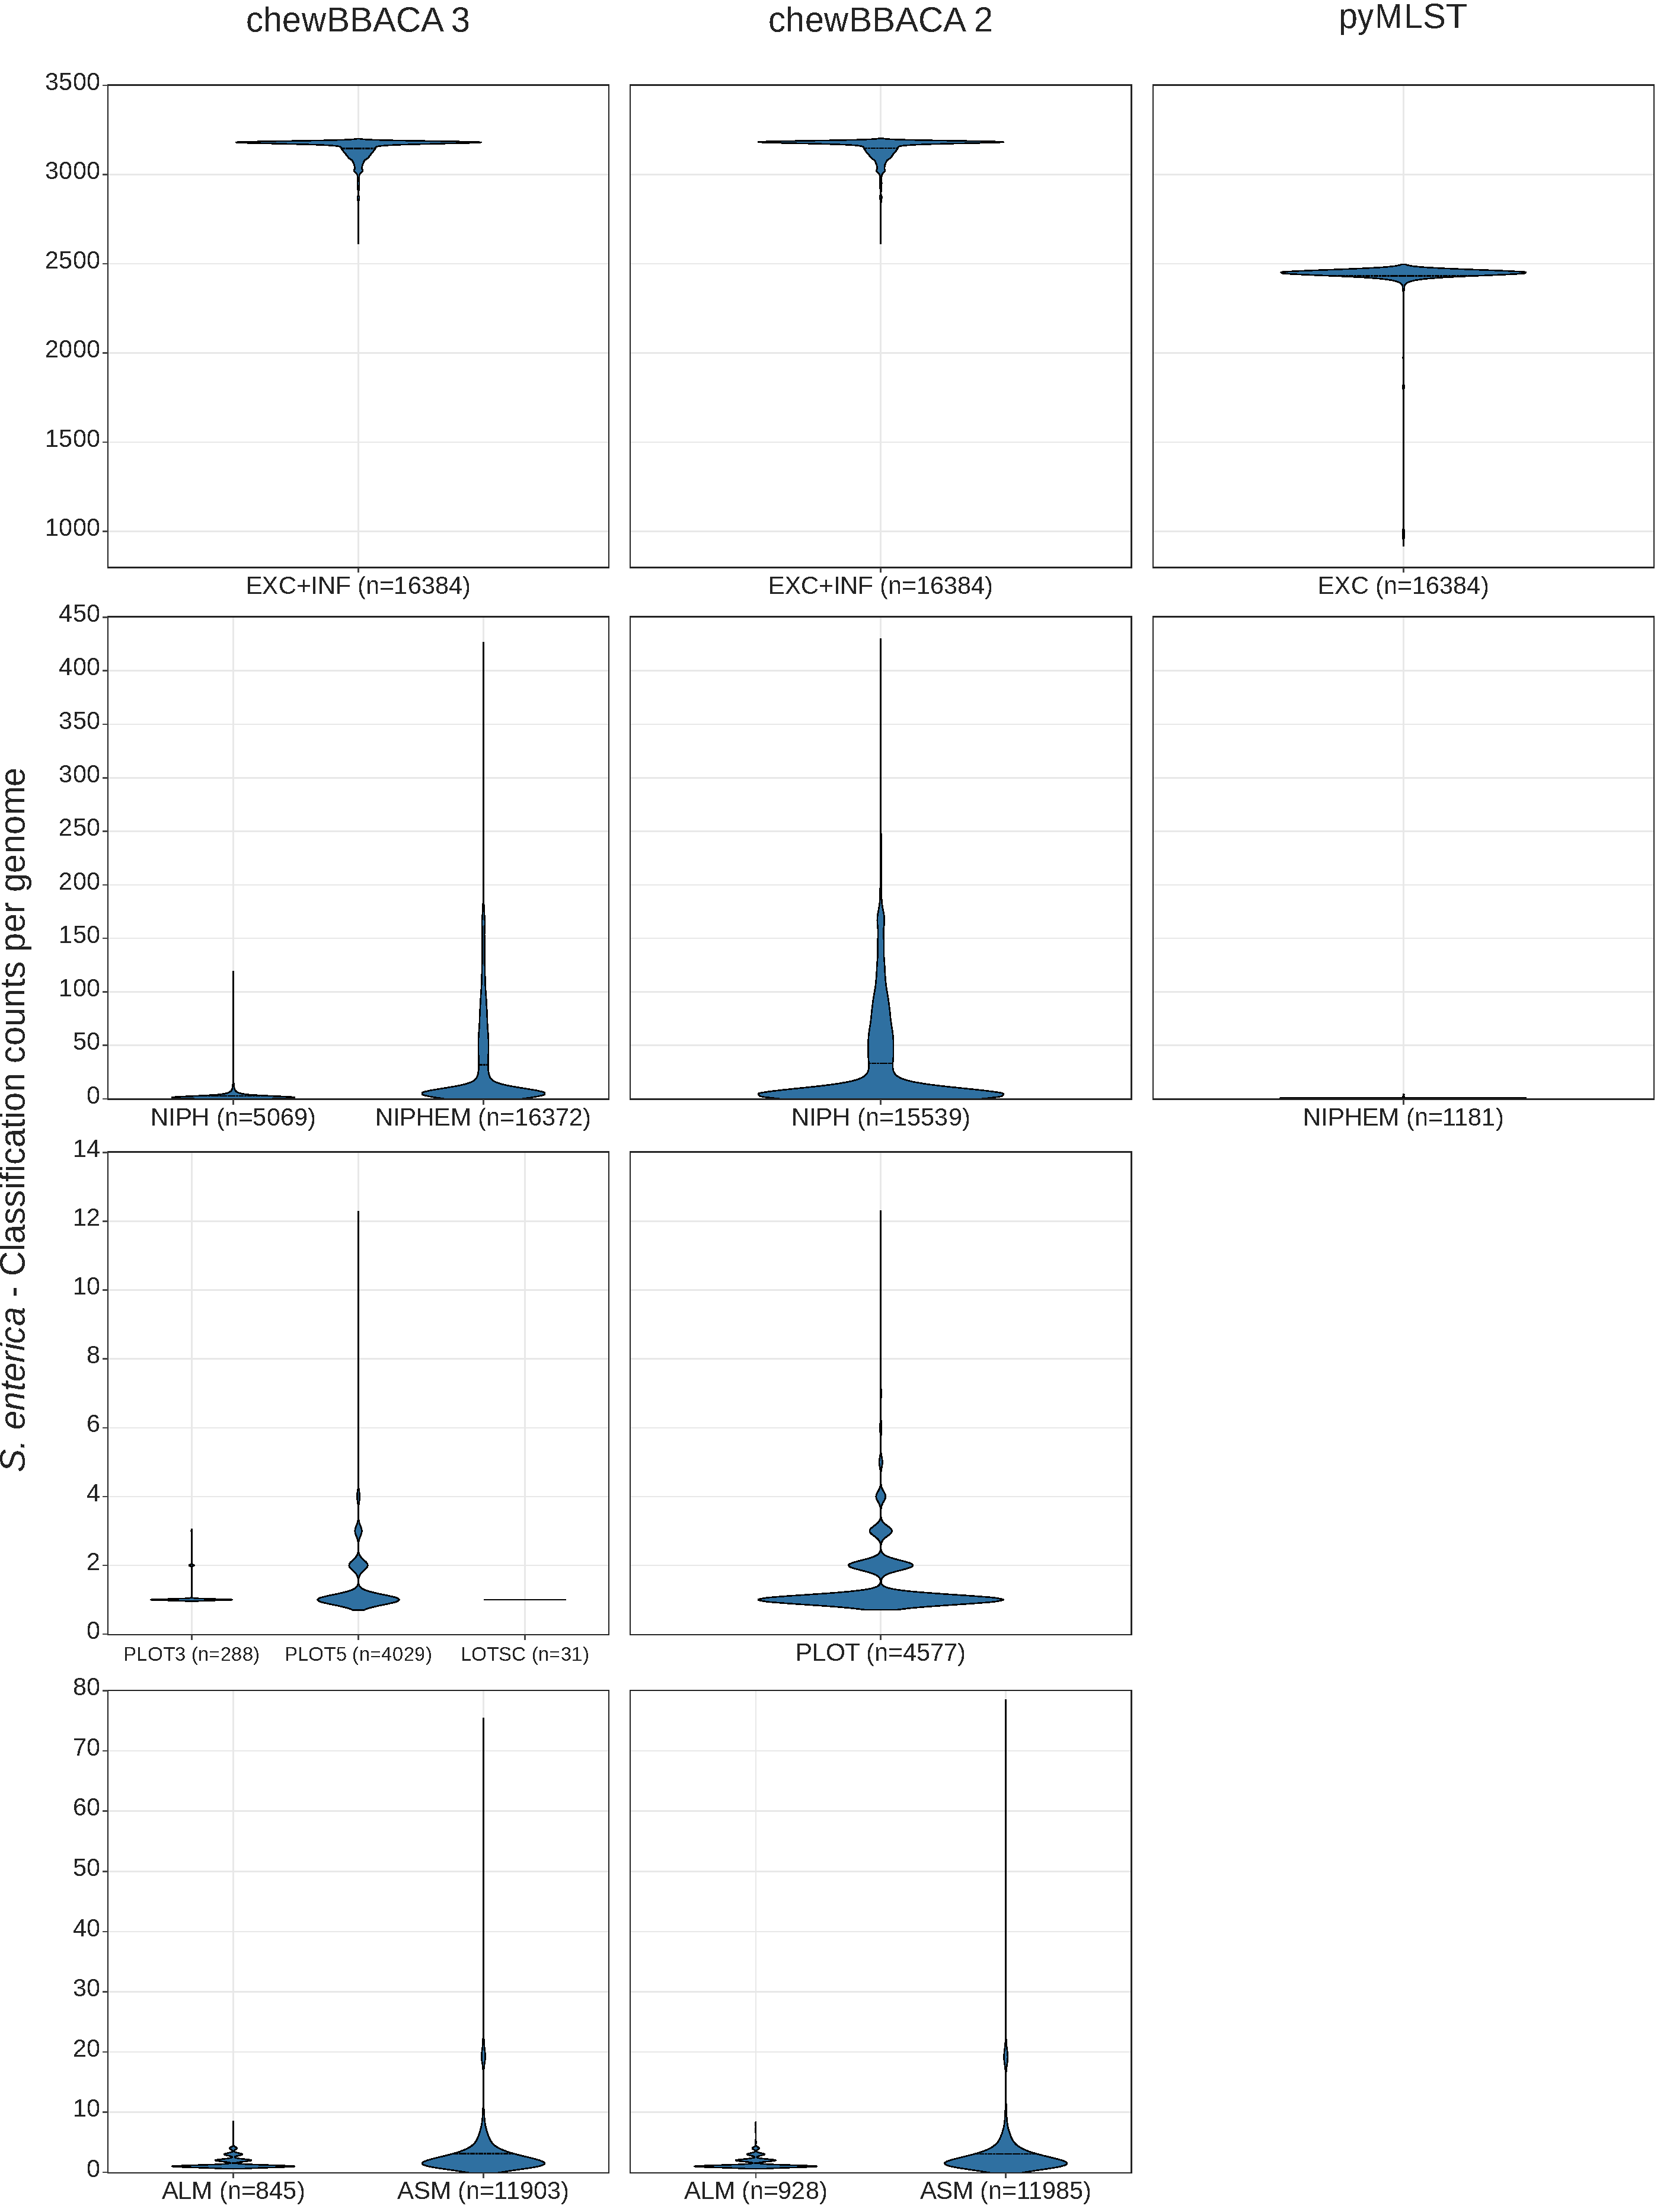
\includegraphics[angle=0,width=\textwidth]{figures/chapter 2/FigureS19.pdf}
    \caption{Classifications counts for the complete dataset (n=16,384 genomes) of S. enterica per tool. Each row displays the counts for the special classifications that are equivalent between tools. The x-axis labels show the names of the classifications and the number of genomes with a count above zero inside the parentheses (i.e. genomes with a count of zero for any of the classifications are not included in the plotted values). For pyMLST, the loci with a single matching CDS were converted to EXC and the loci with multiple matches were converted to NIPHEM. The plot is not shown if the tool does not determine a special classification equivalent to the ones displayed in the row.}
    \label{fig:chap2_figureS19}
\end{figure*}

\newpage
\begin{figure*}[h!]
    \centering
    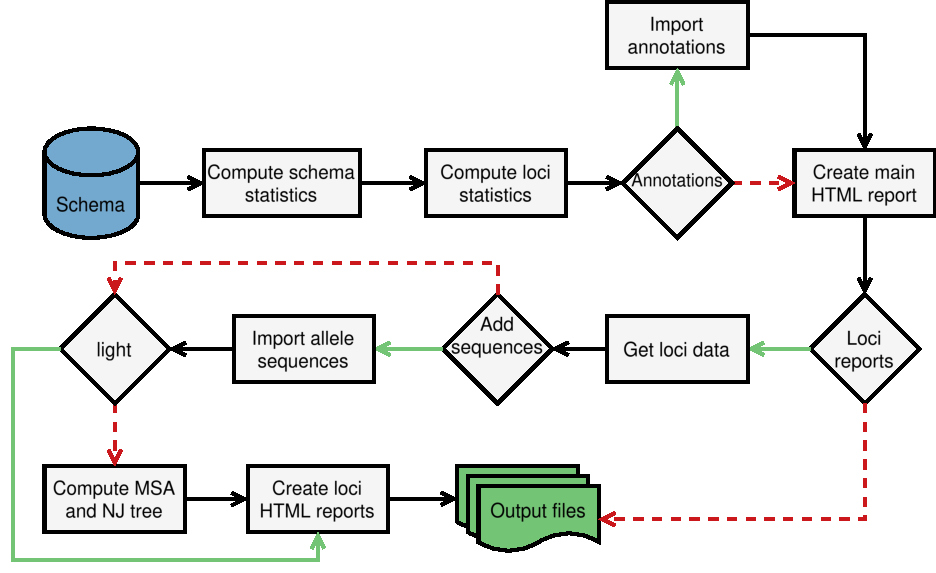
\includegraphics[angle=0,width=\textwidth]{figures/chapter 2/FigureS20.pdf}
    \caption{Diagram of the SchemaEvaluator module. The SchemaEvaluator module analyses a schema to create a report that allows users to explore schema structure and loci diversity interactively. The process starts by computing schema statistics, such as the number of loci and alleles, and loci statistics, such as the number of alleles, allele size statistics, and the number of valid and invalid alleles (e.g. alleles that cannot be translated due to being incomplete, containing ambiguous bases, in-frame stop codons, etc.). The schema and loci statistics are included in interactive data tables and charts on the main page of the HTML report. Loci annotations are imported and included in the main page of the report if provided. If the --loci-reports option is provided, the process performs a detailed analysis of each locus to add a separate locus page to the HTML report for each locus. Loci data is analyzed in greater detail to get more detailed statistics per locus. If the --add-sequences option is provided, the allele DNA sequences are imported and translated to add DNA and protein sequences to code editors on the locus page, which facilitates identifying and manipulating alleles of interest. Additionally, the process computes a multiple sequence alignment (MSA) for each locus at the protein level with MAFFT to display the MSA and MAFFT's guide tree on interactive components. The MSA and guide tree are not displayed if the --light option is provided. The green document icons represent output files. Grey rectangle icons represent analysis steps. Diamond icons represent conditional statements, with green arrows used when the condition is met and red dashed arrows otherwise. The blue cylinder icon represents a schema.}
    \label{fig:chap2_figureS20}
\end{figure*}

\newpage
\begin{figure*}[h!]
    \centering
    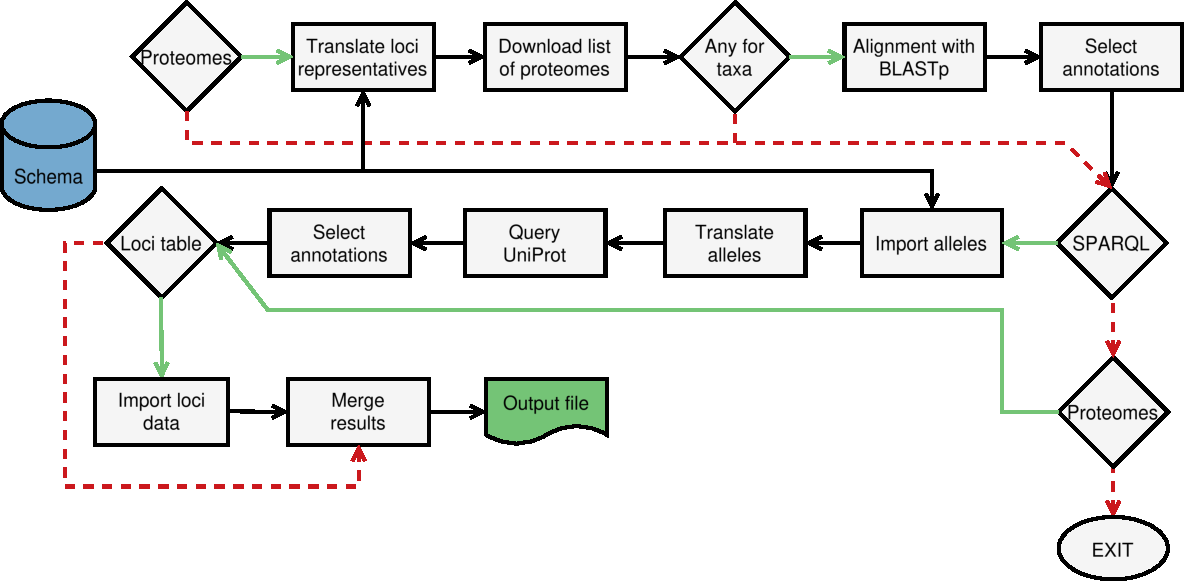
\includegraphics[angle=0,width=\textwidth]{figures/chapter 2/FigureS21.pdf}
    \caption{Diagram of the UniprotFinder module. The UniprotFinder module determines annotations for schema loci. The module offers two options to determine annotations: aligning against UniProt's reference proteomes and exact matching through UniProt's SPARQL endpoint. Users must provide at least one valid taxon name to annotate based on the reference proteomes. The process downloads the list of reference proteomes and searches for proteomes for the specified taxa. If there are any proteomes for the specified taxa, they are downloaded, and the loci representative alleles are aligned against the reference proteomes so annotations can be selected based on the BSR. The process searches for annotations through UniProt's SPARQL endpoint by creating queries including the loci alleles and submitting requests to the endpoint. If an allele matches any protein in UniProt, the annotation terms are extracted from the results. The process tries to select the most informative annotation terms. The annotation terms found through both options are merged to create a single annotations table. If the user provides a TSV file with additional loci data, such as the file with CDS coordinates created by the CreateSchema and AlleleCall modules, the process will add the data in that file to the annotations table. The green document icon represents the output file. Grey rectangle icons represent analysis steps. Diamond icons represent conditional statements, with green arrows used when the condition is met and red dashed arrows otherwise. The blue cylinder icon represents a schema.}
    \label{fig:chap2_figureS21}
\end{figure*}

\newpage
\begin{figure*}[h!]
    \centering
    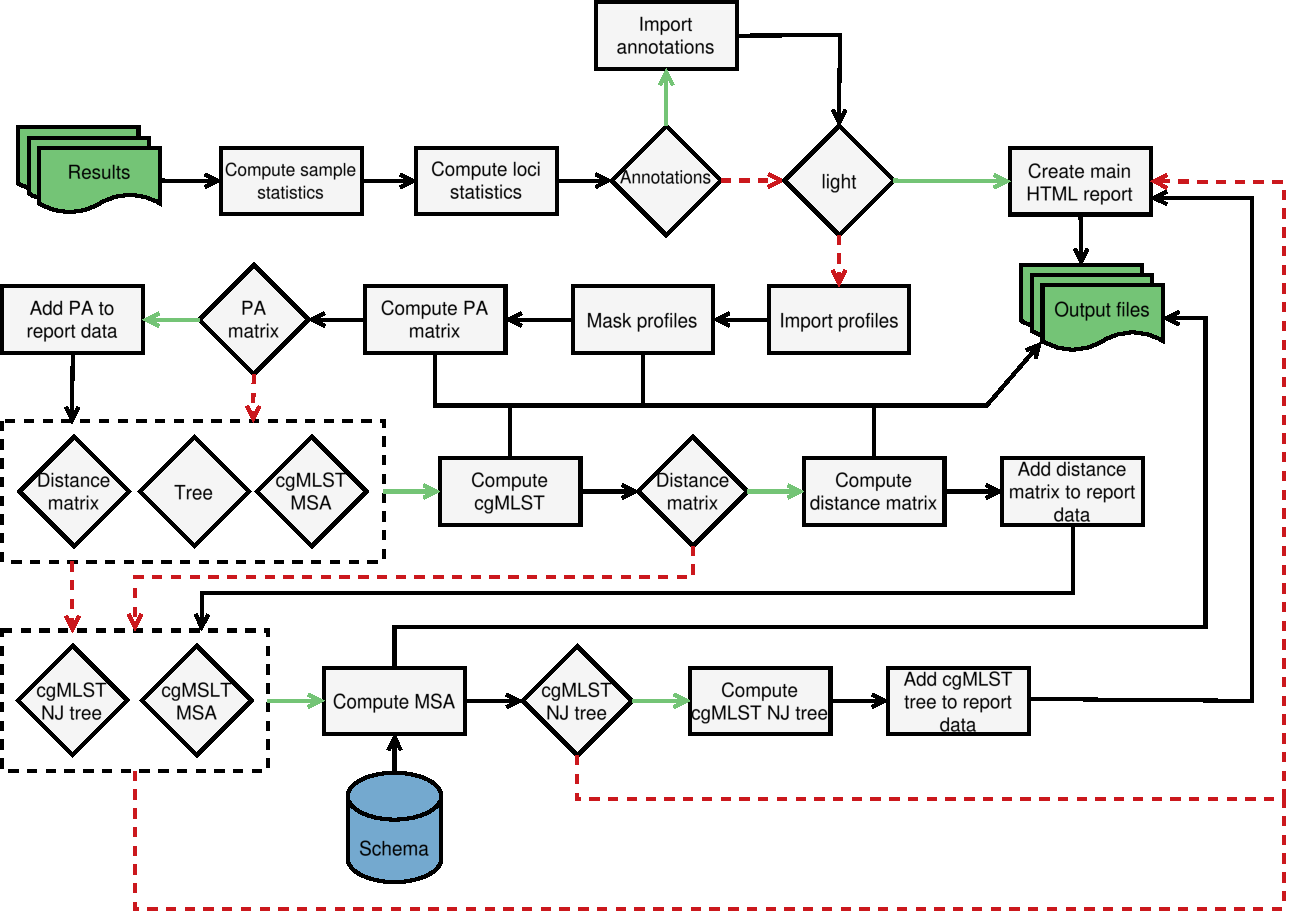
\includegraphics[angle=0,width=\textwidth]{figures/chapter 2/FigureS22.pdf}
    \caption{Diagram of the AlleleCallEvaluator module. The AlleleCallEvaluator module analyses allele calling results to create a report that allows users to explore results interactively. The process starts by importing and computing sample and loci statistics based on the allele calling results. The sample and loci statistics are included in interactive data tables and charts on the main page of the HTML report. Loci annotations are imported and included in the main page of the report if provided. If the --light option is provided, the process does not add more information to the report. Otherwise, the allelic profiles are imported and masked to remove INF- prefixes and substitute special classifications by 0. The masked profiles serve as the basis for computing a presence-absence (PA) matrix, enabling the determination of the set of loci that constitute the core genome. The profile data for the core loci are used to compute a matrix of allelic distances. The core loci alleles identified per strain and locus are imported to compute the cgMLST alignment that FastTree uses to compute a Neighbour-Joining (NJ) tree. The PA and distance matrices and NJ tree data are included in the report to be displayed and explored interactively. The green document icons represent input and output files. Grey rectangle icons represent analysis steps. Diamond icons represent conditional statements, with green arrows used when the condition is met and red dashed arrows otherwise. The blue cylinder icon represents a schema.}
    \label{fig:chap2_figureS22}
\end{figure*}

\begin{landscape}
\vspace*{\fill}
\begin{table}[h!]
    \caption{Runtime (in minutes, min) and peak memory usage (in megabytes, MB) values for the creation of the schema seeds with chewBBACA 2 and chewBBACA 3 based on the complete genomes for each species.}
    \label{tab:ch2_tableS1}
    \centering
    \resizebox{\linewidth}{!}{%
    \small
    \begin{tabular}{@{}lllllllllllllllllll@{}}
    \toprule
    \multicolumn{1}{|c|}{} & \multicolumn{10}{|c|}{chewBBACA 3} & \multicolumn{6}{|c|}{chewBBACA 2} & \multicolumn{2}{|c|}{pyMLST} \\ \midrule
    Species & EXC & INF & PLOT3 & PLOT5 & LOTSC & NIPH & NIPHEM & ALM & ASM & PAMA & EXC & INF & PLOT & NIPH & ALM & ASM & EXC & NIPHEM \\ \hline
    \textit{S. pyogenes} & 21735280 & 218736 & 221 & 1817 & 98 & 154 & 1757 & 1170 & 20841 & 0 & 21736576 & 218665 & 2370 & 504 & 1210 & 20994 & 19078994 & 31 \\ \hline
    \textit{L. monocytogenes} & 38543696 & 538769 & 78 & 5594 & 59 & 23357 & 918118 & 690 & 21541 & 0 & 38552279 & 538435 & 6349 & 932267 & 1149 & 21611 & 23342559 & 289 \\ \hline
    \textit{S. enterica} & 50639542 & 919227 & 308 & 5770 & 31 & 14416 & 523022 & 1309 & 37156 & 31 & 50663361 & 916359 & 6806 & 517896 & 1437 & 36854 & 39838200 & 1200 \\
    \bottomrule
    \end{tabular}%
    }
\end{table}
\vspace*{\fill}
\end{landscape}



% \begin{landscape}
% \begin{table}[]
\caption{Microorganisms identified by conventional methods, \ac{WGS} and using shotgun metagenomics and the taxonomic classification methods in Unix.}
\label{tab:ch2_table2}
\resizebox{\linewidth}{!}{%
\begin{tabular}{@{}|l|l|l|l|lll|@{}}
\toprule
\multicolumn{1}{|c|}{\multirow{2}{*}{\textbf{Sample number}}} &
  \multicolumn{1}{c|}{\multirow{2}{*}{\textbf{Culture result (CFU)$^a$}}} &
  \multicolumn{1}{c|}{\multirow{2}{*}{\textbf{\begin{tabular}[c]{@{}c@{}}Conventional identification\\  (MALDI-TOF)\end{tabular}}}} &
  \multicolumn{1}{c|}{\multirow{2}{*}{\textbf{\ac{WGS}-based identification}}} &
  \multicolumn{3}{c|}{\textbf{Shotgun metagenomics}} \\ \cmidrule(l){5-7} 
\multicolumn{1}{|c|}{} &
  \multicolumn{1}{c|}{} &
  \multicolumn{1}{c|}{} &
  \multicolumn{1}{c|}{} &
  \multicolumn{1}{c|}{\textbf{Kraken$^b$}} &
  \multicolumn{1}{c|}{\textbf{MIDAS$^c$}} &
  \multicolumn{1}{c|}{\textbf{MetaPhlAn$^c$}} \\ \midrule
\textbf{1} &
  \begin{tabular}[c]{@{}l@{}}10$^3$\\  10$^3$\\  10\end{tabular} &
  \begin{tabular}[c]{@{}l@{}}\textit{E. faecium}\\  \textit{S. haemolyticus}\\  \textit{C. glabrata}\end{tabular} &
  \begin{tabular}[c]{@{}l@{}}\textit{E. faecium}\\  \textit{S. haemolyticus}\\  -\end{tabular} &
  \multicolumn{1}{l|}{\begin{tabular}[c]{@{}l@{}}\textit{E. faecium} (34.6\%)\\  \textit{S. haemolyticus} (10.1\%)\\  -\end{tabular}} &
  \multicolumn{1}{l|}{\begin{tabular}[c]{@{}l@{}}\textit{E. faecium} (62.0\%)\\  \textit{S. haemolyticus} (28.0\%)\\  -\end{tabular}} &
  \begin{tabular}[c]{@{}l@{}}\textit{E. faecium} (66.6\%)\\  \textit{S. haemolyticys} (27.7\%)\\  -\end{tabular} \\ \midrule
\textbf{2} &
  \begin{tabular}[c]{@{}l@{}}10$^3$\\  1\\  Not determined\end{tabular} &
  \begin{tabular}[c]{@{}l@{}}\textit{E. avium}\\  \textit{E. coli}\\  Anaerobes\end{tabular} &
  \begin{tabular}[c]{@{}l@{}}-\#\\  -\#\\  -\#\end{tabular} &
  \multicolumn{1}{l|}{\begin{tabular}[c]{@{}l@{}}Not identified$^*$\\  Not identified$^*$\\  Several species (29.5\%)\end{tabular}} &
  \multicolumn{1}{l|}{\begin{tabular}[c]{@{}l@{}}Not identified$^*$\\  Not identified$^*$\\  Several species (100.0\%)\end{tabular}} &
  \begin{tabular}[c]{@{}l@{}}Not identified$^*$\\  Not identified$^*$\\  Several species (100.0\%)\end{tabular} \\ \midrule
\textbf{3} &
  1 &
  \textit{S. epidermidis} &
  -$^\#$ &
  \multicolumn{1}{l|}{S. aureus (0.2\%)} &
  \multicolumn{1}{l|}{Not identified$^*$} &
  Not identified$^*$ \\ \midrule
\textbf{4} &
  10$^3$ &
  \textit{S. aureus} &
  \textit{S. aureus} &
  \multicolumn{1}{l|}{\textit{S. aureus} (0.73\%)} &
  \multicolumn{1}{l|}{\textit{S. aureus }(100\%)} &
  \textit{S. aureus} (100\%) \\ \midrule
\textbf{5} &
  \begin{tabular}[c]{@{}l@{}}$\geq$ 10$^5$\\  $\geq$ 10$^5$\\  10$^3$\\  10$^3$\\  Not determined\\  10\end{tabular} &
  \begin{tabular}[c]{@{}l@{}}\textit{E. coli}\\  \textit{K. oxytoca}\\  \textit{S. anginosus}\\  \textit{E. faecalis}\\  Anaerobes\\  \textit{C. albicans}\end{tabular} &
  \begin{tabular}[c]{@{}l@{}}\textit{E. coli}\\  \textit{K. oxytoca}\\  -$^\#$\\  \textit{E. faecalis}\\  -$^\#$\\  -$^\#$\end{tabular} &
  \multicolumn{1}{l|}{\begin{tabular}[c]{@{}l@{}}\textit{E. coli} (9.7\%)\\  \textit{K. oxytoca} (0.5\%)\\  \textit{S. anginosus} (0.07\%)\\  \textit{E. faecalis} (0.3\%)\\  Several species (12.7\%)\\  -\end{tabular}} &
  \multicolumn{1}{l|}{\begin{tabular}[c]{@{}l@{}}\textit{E. coli} (6.5\%)\\  \textit{K. oxytoca} (0.3\%)\\  \textit{S. anginosus} (0.01\%)\\  \textit{E. faecalis} (0.9\%)\\  Several species (96.7\%)\\  -\end{tabular}} &
  \begin{tabular}[c]{@{}l@{}}\textit{E. coli} (8.5\%)\\  \textit{K. oxytoca} (0.3\%)\\  \textit{Streptococcus spp.} (0.09\%)\\  \textit{E. faecalis} (0.7\%)\\  Several species (90.4\%)\\  -\end{tabular} \\ \midrule
\textbf{6} &
  10$^3$ &
  \textit{E. faecium} &
  \textit{E. faecium} &
  \multicolumn{1}{l|}{\textit{E. faecium} (0.77\%)} &
  \multicolumn{1}{l|}{Not identified$^*$} &
  Not identified$^*$ \\ \midrule
\textbf{7} &
  10$^2$ &
  \textit{S. aureus} &
  -$^\#$ &
  \multicolumn{1}{l|}{\textit{S. aureus} (82.9\%)} &
  \multicolumn{1}{l|}{\textit{S. aureus} (100\%)} &
  \textit{S. aureus} (100\%) \\ \midrule
\textbf{8} &
  10$^3$ &
  \textit{O. intermedium} &
  \textit{O. intermedium} &
  \multicolumn{1}{l|}{\textit{O. anthropi} (21.3\%)} &
  \multicolumn{1}{l|}{\textit{O. intermedium} (99.4\%)} &
  \textit{O. intermedium} (99.1\%) \\ \midrule
\textbf{9} &
  10$^3$ &
  \textit{S. aureus} &
  \textit{S. aureus} &
  \multicolumn{1}{l|}{\textit{S. aureus} (22.9\%)} &
  \multicolumn{1}{l|}{\textit{S. aureus} (100\%)} &
  \textit{S. aureus} (100\%) \\ \midrule
\textbf{10} &
  10$^3$ &
  \textit{S. marcescens} &
  -\# &
  \multicolumn{1}{l|}{\textit{S. marcescens} (64.7\%)} &
  \multicolumn{1}{l|}{\textit{S. marcescens} (99.1\%)} &
  \textit{S. marcescens} (100\%) \\ \bottomrule
\end{tabular}%
}
\small
\item $^a$The number of colonies of a given species was estimated from the number of colonies with the same morphology on the same plate 
\item $^b$The relative abundance is calculated using total number of reads as denominator
\item $^c$The relative abundance is calculated with the total number of classified reads as denominator
\item $^d$miniKraken database was used
\item $^\#$Although there was a laboratory identification, no isolates were available for \ac{WGS}
\item $^*$No reads matched that specific pathogen, not even at the genus level
\end{table}
% \end{landscape}


%-----------------------------------------------------------------
% Paper 2 - Chewie-NS
%------------------------------------------------------------------
\newpage
\thispagestyle{empty}
\chapter{Chewie Nomenclature Server (Chewie-NS): a deployable nomenclature server for easy sharing of core and whole genome MLST schemas\label{ch:paper2}}
\thispagestyle{empty}
\cleardoublepage
\mbox{}\\
\vspace{8cm}

This chapter is a reproduction of the following publication:

R. Mamede, P. Vila-Cerqueira, M. Silva, J. A. Carriço, M. Ramirez, Chewie Nomenclature Server (Chewie-NS): a deployable nomenclature server for easy sharing of core and whole genome MLST schemas, Nucleic Acids Research, Volume 49, Database Issue, January 2021, D660-D666, DOI: \url{https://doi.org/10.1093/nar/gkaa889}

The adoption of \ac{wg/cgMLST} has been largely driven by the availability of web platforms that provide powerful analytic capabilities for \ac{wg/cgMLST} and centralize data analysis, ensuring the standardization of data analysis steps and the comparability of the results. These platforms store genomic and gene sequences, as well as associated metadata, and allow users to identify loci and alleles present in submitted strains based on comparisons against \ac{wg/cgMLST} schemas with well-defined allelic nomenclatures. These centralized services greatly promote interoperability and provide a richer context by allowing users to compare their strains against strains submitted by other users from diverse geographic locations. However, by requiring users to submit their data and centralizing data analysis, the services provided by these platforms may not be adequate for users operating under strict data privacy policies and may offer limited scalability, especially as data availability increases and when a timely analysis is desirable, such as in an outbreak context.

This chapter presents \ac{Chewie-NS}, a deployable \ac{wg/cgMLST} platform for easy sharing of \ac{wg/cgMLST} schemas that allows users to perform local and private analysis under a common allelic nomenclature. \ac{Chewie-NS} was designed to store \ac{wg/cgMLST} schemas for any bacterial species and to provide a simple user interface for users to intuitively explore the diversity of loci included in each schema. Schema and loci data can be easily browsed and downloaded through the website or \ac{API}. Furthermore, integration with chewBBACA 3, presented in \textbf{\autoref{ch:paper1}}, allows users to quickly download schemas and start performing local and private analyzes based on the common allelic nomenclature managed by \ac{Chewie-NS}. By decentralizing data analysis, users operating under strict data privacy policies can still use \ac{Chewie-NS}' services, and data processing is not limited by the resources available to the remote server.

As first co-author, I was involved in the implementation of the backend component and of the modules that allow for the integration with chewBBACA 3. My contribution to the Frontend component consisted of the creation of Python scripts that generate pre-computed data to be displayed in the tables and plots of the website. The development of \ac{Chewie-NS} was in part guided by a proof of concept that had been previously implemented by members of the lab where the work was carried out. I focused mainly on defining and creating the endpoints of the \ac{API} and on making sure that the \ac{API} provided the functionalities necessary for the integration with chewBBACA and the Frontend component. I developed the \ac{API} and the modules for integration with chewBBACA 3 simultaneously to ensure that they were fully compatible. In addition, I had to fine-tune and optimize several \ac{API} endpoints, restructure the database used to store schema data and create custom Python scripts to guarantee that \ac{Chewie-NS} provided the desired functionalities at scale.

\newpage

\begin{center}
\large
\textbf{Chewie Nomenclature Server (Chewie-NS): a deployable nomenclature server for easy sharing of core and whole genome MLST schemas}
\end{center}

Rafael Mamede$^{1,2}$, 
Pedro Vila-Cerqueira$^1$, 
Mickael Silva$^1$,
João A. Carriço$^1$,
Mário Ramirez$^1$,

$^1$ Instituto de Microbiologia, Instituto de Medicina Molecular, Faculdade de Medicina, Universidade de Lisboa, Portugal;

$^2$ Gulbenkian Institute for Molecular Medicine.

\section{Abstract} \label{sec:ch3_abstract}

\ac{Chewie-NS} (\url{https://chewbbaca.online/}) allows users to share genome-based gene-by-gene typing schemas and to maintain a common nomenclature, simplifying the comparison of results. The combination between local analyses and a public repository of allelic data strikes a balance between potential confidentiality issues and the need to compare results. The possibility of deploying private instances of \ac{Chewie-NS} facilitates the creation of nomenclature servers with a restricted user base to allow compliance with the strictest data policies. \ac{Chewie-NS} allows users to easily share their own schemas and to explore publicly available schemas, including informative statistics on schemas and loci presented in interactive charts and tables. Users can retrieve all the information necessary to run a schema locally or all the alleles identified at a particular locus. The integration with the chewBBACA suite enables users to directly upload new schemas to \ac{Chewie-NS}, download existing schemas and synchronize local and remote schemas from chewBBACA command line version, allowing an easier integration into high-throughput analysis pipelines. The same \ac{REST} \ac{API} linking \ac{Chewie-NS} and the chewBBACA suite supports the interaction of other interfaces or pipelines with the databases available at \ac{Chewie-NS}, facilitating the reusability of the stored data.

\section{Introduction} \label{sec:ch3_introduction}

The importance of distinguishing strains within the same microbial species has been proven critical for identifying chains of transmission and understanding pathogen evolution, as recently illustrated by the SARS-CoV-2 pandemic \cite{black_ten_2020, deng_genomic_2020}. The advent and widespread adoption of high-throughput sequencing allowed leveraging genomic information for this purpose \cite{black_ten_2020, deng_genomic_2020}. One of the most common approaches in bacterial typing is \ac{GbG} methods, which extend the concept of \ac{MLST} to include all genes present in the core genome of a given species (\ac{cgMLST}) or, trying to cover a significant fraction of a species’ pan-genome, in whole genome (\ac{wgMLST}) \cite{maiden_mlst_2013}. Current software approaches implementing these \ac{wg/cgMLST} typing methods suffer from standardization issues when comparing results between different tools and between different laboratories or users \cite{uelze_typing_2020}.

We have previously developed a suite, chewBBACA \cite{silva_chewbbaca_2018}, allowing the creation of \ac{GbG} schemas and performing allele calls on assembled draft genomes. Since chewBBACA was designed to perform local analysis to address concerns over data privacy and scalability, it has the drawback that small adjustments in parameters may lead to inconsistencies between runs. Moreover, the software allows users to create their own \ac{wg/cgMLST} schemas but currently no tool is available for the easy sharing of schemas, which potentially hampers long-term and multinational studies, as well as the reusability of already published schemas \cite{isidro_virulence_2020, llarena_innuendo_2018}.

There are well-established websites for performing \ac{GbG} analyses, such as PubMLST (\url{https://pubmlst.org/}) \cite{jolley_bigsdb_2010} and EnteroBase (\url{https://enterobase.warwick.ac.uk/}) \cite{zhou_enterobase_2020}, that centralize analysis and hosting of public and private schemas. chewBBACA does not depend on a web server and by enabling local analyses and schema creation allows for scalable and private analyses of genomes, but the existing implementation lacked an easy way to share schemas and the associated allelic information, which is possible in a centralized solution.

In order to allow users to share \ac{GbG} typing schemas and for a common allelic nomenclature to be maintained \cite{carrico_bioinformatics_2013}, we developed \ac{Chewie-NS}, a nomenclature server based on the TypOn ontology \cite{vaz_typon_2014} offering a web interface that also integrates directly with local instances of chewBBACA and can be programmatically accessed by external resources. \ac{Chewie-NS} aims to complement the private local analysis of strains by also allowing the simple communication of results while providing an interface for users to easily explore the allelic diversity within species. The importance of the latter is becoming increasingly clear with the recognition that bacterial phenotypes can be profoundly altered by allelic variants \cite{van_der_linden_heterogeneity_2020, uniprot_consortium_uniprot_2019}. Other publicly available web services require submission of raw data, something that may raise privacy and ownership concerns, while our approach of enabling local analyses is more flexible and scalable, and respects data privacy concerns. Current \ac{wg/cgMLST} typing methods suffer from standardization difficulties or issues that manifest not only when trying to reconcile results from different tools, but also when the same tool is run at different times with small adjustments in parameter values or database modifications that may lead to inconsistencies. This is an even more complex problem than it was for classical \ac{MLST} methods \cite{page_comparison_2017}. Having a repository of schemas, their associated parameters and the allelic diversity identified will allow the consistent use of gene-by-gene typing schemas by different groups and to build upon the results of different studies to monitor microbial populations and study outbreaks.

\ac{Chewie-NS} is available at \url{https://chewbbaca.online} and its source code is available at \url{https://github.com/B-UMMI/Chewie-NS}. Detailed documentation, including a descriptive tutorial on how to deploy and use the server, can be found at \url{https://chewie-ns.readthedocs.io}. Additionally, a tutorial version of the server aiming at familiarizing users with the integration between the chewBBACA suite and \ac{Chewie-NS}, which allows users to perform mock submissions of schemas and synchronizations without the need to register and with a much reduced database, is available at \url{https://tutorial.chewbbaca.online/}.

\section{Database Creation} \label{sec:ch3_database_creation}

\subsection{Backend} \label{ssec:ch3_database_creation_backend}

The architecture of \ac{Chewie-NS} is shown schematically in \ref{fig:chap3_figure1}. The backend component of \ac{Chewie-NS} makes use of the Virtuoso triple store (v. 7.2.6) (\url{https://virtuoso.openlinksw.com/}). This database management system allows the integration of a \ac{RDF} to implement the TypOn ontology \cite{vaz_typon_2014} structure to store schema data. Additionally, a PostgreSQL database (v. 10) (\url{https://www.postgresql.org/}) was adopted for user management. These databases are accessible through a Python 3 \ac{REST} \ac{API} developed in the Flask (v. 1.1.0) (\url{https://flask.palletsprojects.com/en/1.1.x/}) web development microframework, which allows requests through defined endpoints and facilitates programmatic access to the nomenclature server. Requests and \ac{HTTPS} connections are handled by a web server, NGINX (v. 1.17) (\url{https://www.nginx.com/}), that communicates with Gunicorn (v. 20.0.4) (\url{https://gunicorn.org/}), a \ac{WSGI} application server capable of running multiple processes of the web application and distributing incoming requests to ensure scalability and load balancing. A queueing system was implemented to manage all tasks with possible concurrent user access through Redis (v. 5.0.6) (\url{https://redis.io/}) and Celery (v. 4.4.0rc2) (\url{https://docs.celeryproject.org/en/stable/getting-started/introduction.html}).

\subsection{Frontend} \label{ssec:ch3_database_creation_frontend}

The \ac{UI} for \ac{Chewie-NS} was built with the JavaScript frameworks React (v. 16.12.0) (\url{https://reactjs.org/}) and Material-UI (v. 4.9.14) (\url{https://material-ui.com/}). The \ac{UI} provides a list of available schemas and displays relevant schema and locus statistics in a responsive and interactive manner. Access to daily updated compressed files of the schemas for download and local use is also provided. All interactive charts were rendered with the graph visualization library Plotly.js (v. 1.52.1) (\url{https://plotly.com/javascript/}) through its React component, react-plotly (v.2.4.0) (\url{https://plotly.com/javascript/react/}).

\newpage
\begin{landscape}
\vspace*{\fill}
\begin{figure*}[!ht]
    \centering
    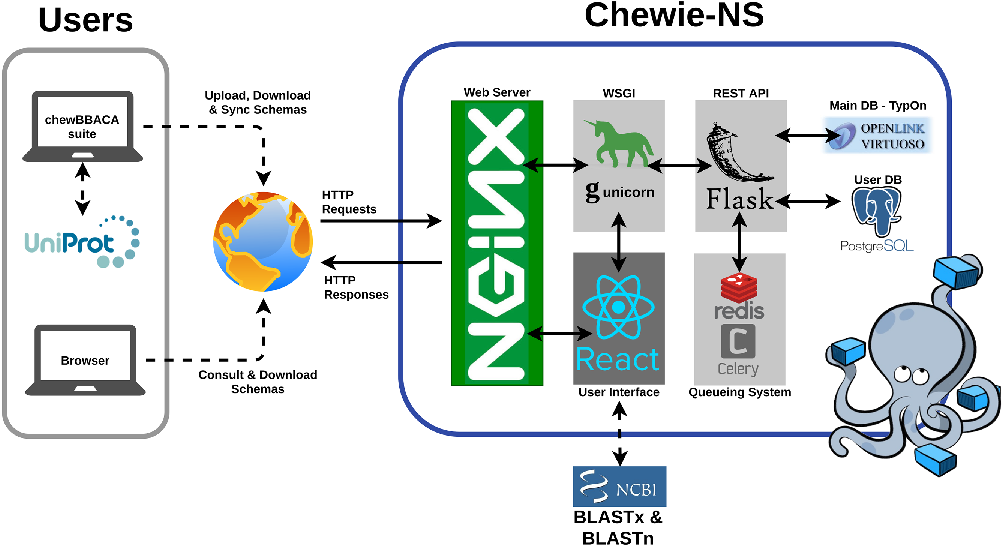
\includegraphics[width=20cm]{figures/chapter 3/Figure1.pdf}
    \caption[The Chewie-NS service: global overview of the technologies used and API connectivity.]{The Chewie-NS service: global overview of the technologies used and API connectivity.}
    \label{fig:chap3_figure1}
\end{figure*}
\vspace*{\fill}
\end{landscape}

\subsection{Chewie-NS usage} \label{ssec:ch3_database_creation_usage}

\textit{Local installation}. Deployment of local instances can be easily achieved through Docker Compose (\url{https://www.docker.com/}), available at \url{https://github.com/B-UMMI/Chewie-NS}. The use of a container orchestrator (\url{https://docs.docker.com/compose/}) supports the easy deployment of local instances independently of the hardware available, allowing the creation of private trusted databases if public access is not possible. Instructions on how to achieve this can be found at \url{https://github.com/B-UMMI/Chewie-NS}. This can be particularly important for national public health institutions in the context of restrictive or ambiguous data sharing laws because it allows stricter user access control.

\textit{Application programming interface}. A \ac{REST}ful \ac{API} also referred to as a \ac{REST}ful web service or \ac{REST} \ac{API}, i.e. based on representational state transfer (REST), is available. The user can interact with \ac{Chewie-NS}’s \ac{API} through the web interface, by clicking on the ‘API’ button on the menu. This will open a page with Swagger \ac{UI} (\url{https://swagger.io/tools/swagger-ui/}), a user-friendly tool for the user to interact directly with the \ac{REST} \ac{API}. Programmatic access is also possible through command line applications such as curl or tools such as Postman (\url{https://www.postman.com/}). \ac{Chewie-NS}’s \ac{REST} \ac{API} allows interaction with the PostgreSQL database to manage user registrations on local instances. Through the \ac{API}, users are also able to query the Virtuoso database to download compressed schemas, search for specific alleles and query data about specific species, loci or alleles.

\subsection{Web interface} \label{ssec:ch3_database_creation_interface}

\textit{Schemas overview}. A table summarizes the species and number of schemas available for each species in \ac{Chewie-NS}. Selecting a species leads to another table (\ref{fig:chap3_figure2}) with a list of relevant information about each available schema, namely the schema internal identifier, the user provided schema name, the username of the creator, the number of loci in the schema, the number of alleles, the software and version used to create the schema, the date of creation, the date of the last modification, the BLAST \cite{altschul_basic_1990} score ratio selected, the translation table used, the minimum locus length and size threshold. In the table, there is a link to download the compressed file of the schema and the training file used to create it, both necessary to use the schema locally with the chewBBACA suite. Each table entry has also a link to a page containing more details about the schema. Below this table, an interactive bar chart displays the number of alleles per locus for each schema. The user can zoom in on the chart to obtain a better view of a given set of loci and can click on a bar to go to a page with more details on that particular locus.

\begin{figure*}[!ht]
    \centering
    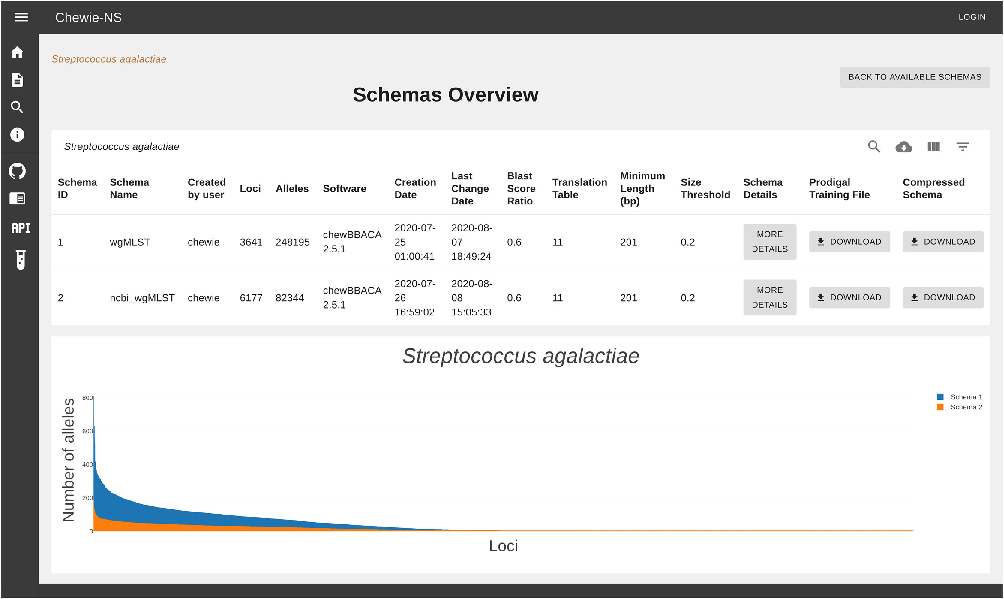
\includegraphics[width=\textwidth]{figures/chapter 3/Figure2.pdf}
    \caption[The schemas overview page of Chewie-NS.]{The schemas overview page of Chewie-NS.}
    \label{fig:chap3_figure2}
\end{figure*}

\textit{Schema details}. The schema evaluation and annotation page contains a description of the schema provided by the schema creator. During the schema upload, this information can be provided in a file using markdown, a simple plain-text-formatting syntax that allows the easy integration of hyperlinks, tables and images, allowing for a rich use of data for the description of the schema. Below this table are four charts in different tabs. Two charts (\ref{fig:chap3_figure3}) display characteristics of the schema: the distribution of the number of alleles per locus and of locus size. Two interactive charts represent for each locus its size summary statistics versus the number of alleles, and another a box plot of the size distribution of each locus. In all charts, the user can zoom in on particular regions for more detailed inspection and, on the latter two, clicking on the chart element opens a page with more information on that particular locus. Below the charts is a table of all the loci in the schema, including relevant information for each locus. This table, as all other tables of \ac{Chewie-NS}, is searchable, facilitating finding loci with particular characteristics (\ref{fig:chap3_figure4}). Similarly to other tables, the table can also be exported in comma-separated values format.

\textit{Locus details}. Already in the schema evaluation and annotation page is shown most of the information of each locus. This includes the internal locus identification and label, the automated annotation created by chewBBACA including a link to the relevant UniProt \cite{uniprot_consortium_uniprot_2019} page, a user locus name and user custom annotation (supporting markdown syntax), number of alleles and allele size information. The possibility of schema creators offering their own annotation allows for domain-specific information to be added to the schema, including potentially richer complementary data and links to relevant external resources. Two charts are offered, one summarizing the size distribution of the alleles (frequency of binned sizes) and the other representing the sizes of each allele. Direct links to perform \ac{BLAST} searches using allele 1 of that locus (\ac{BLASTn} and \ac{BLASTx}) are available at the bottom of the page, allowing the user to check for similarities that could offer further insights into the origin or likely function of the protein potentially encoded by the locus. A multi-fasta file containing the alleles of the locus can be downloaded by the users from this page. On a different page, a simple query feature allows finding exact matches to specific sequences stored in any of \ac{Chewie-NS}’s databases, returning the loci and schemas where the sequence is found.

\begin{figure*}[!ht]
    \centering
    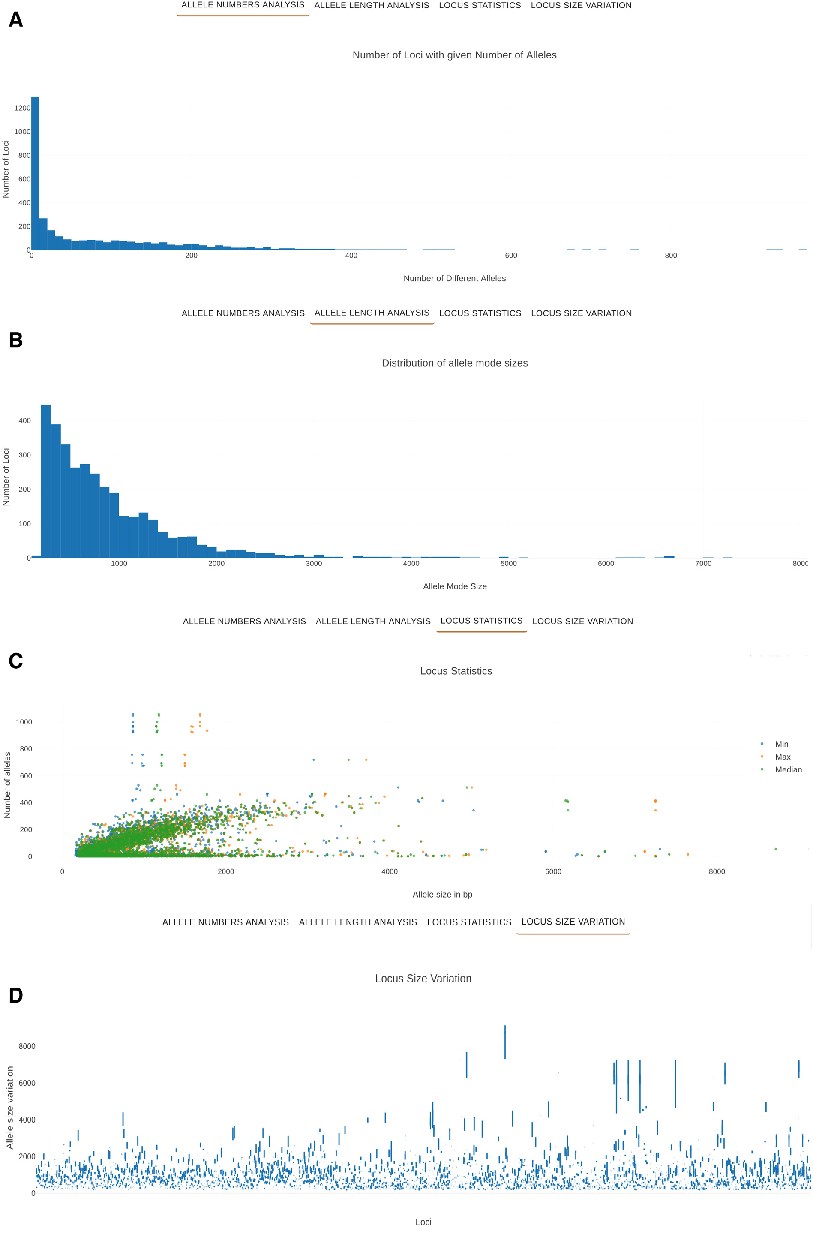
\includegraphics[angle=0,height=0.80\textheight]{figures/chapter 3/Figure3.pdf}
    \caption[Summary charts displaying relevant information on a given schema.]{Summary charts displaying relevant information on a given schema. \textbf{(A)} Distribution of loci by number of alleles. \textbf{(B)} Distribution of loci by allele mode size. \textbf{(C)} Representation of summary statistics (minimum allele size in blue, maximum allele size in orange and median allele size in green) for each locus. \textbf{(D)} Box plots of loci size distribution; the loci in the x-axis are ordered by locus ID.}\label{fig:chap3_figure3}
\end{figure*}

\textit{Integration with the chewBBACA suite and use of the API}. By taking advantage of \ac{Chewie-NS}’s \ac{API}, chewBBACA is capable of handling not only the schema creation, but also its upload, synchronization and download. Users of chewBBACA registered in \ac{Chewie-NS} and with contributor privileges will be able to automatically upload a novel schema, making it available in \ac{Chewie-NS}. Any authorized registered user can also contribute novel alleles identified in local analyses to \ac{Chewie-NS}, contributing to the incremental development of the schema. This involves only allele information without the need to share a complete allelic profile with \ac{Chewie-NS}. On the other hand, one does not have to be registered to download any of the data stored in \ac{Chewie-NS},including the compressed schemas or the novel alleles submitted to the \ac{Chewie-NS} database and that were not present on the compressed file to update the local schema. Detailed instructions on the chewBBACA commands to achieve this can be found at \url{https://chewie-ns.readthedocs.io/en/latest/user/chewbbaca.html}.

If a user creates a schema through a software other than chewBBACA, the \ac{API} can still be used to submit this new schema to \ac{Chewie-NS} or to add novel alleles to non-chewBBACA schemas. A user would have to register with \ac{Chewie-NS} and would have to take on the responsibility for making the correct \ac{API} calls for schema submission. Furthermore, it would be up to each user submitting new alleles to guarantee the consistency of these novel alleles with the schema originally deposited. These functions are handled transparently by chewBBACA in its interaction with \ac{Chewie-NS}. Anyone can use the \ac{API} to download any of the schemas deposited in \ac{Chewie-NS} to be run locally with chewBBACA or any other allele-calling algorithm. These multiple ways in which a user can interact with \ac{Chewie-NS} allows tailoring the sharing of information to user preferences or to restrictions imposed on particular users.

In order to facilitate familiarization of the interaction between chewBBACA and \ac{Chewie-NS}, a tutorial website was created (\url{https://tutorial.chewbbaca.online/}), together with step-by-step instructions on how to perform mock operations with a small size schema (\url{https://chewie-ns.readthedocs.io/en/latest/user/tutorial.html}). This allows users to perform submissions and synchronization of schemas without the need for registering. The schemas submitted to the tutorial site are not permanent and are removed automatically 48 h after creation.

For reproducibility and traceability purposes, a feature to retrieve database snapshots at specific dates is available, allowing a user to be able to recover the exact schema, as it was available on a given date. Full documentation of the schemas allows for traceability, which is critical in public health applications. These various options will continue to allow data privacy, while striving for a common nomenclature. The detailed parameterization associated with each schema created with chewBBACA and the consistency checks implemented in \ac{Chewie-NS} mean that no human curation is necessary after the schema creation step, contributing to the rapid update of the database and exchange of information. However, although \ac{Chewie-NS} can be used to store and retrieve information of schemas not created with chewBBACA, it does not currently automatically guarantee the consistency of newly submitted alleles since each allele-calling algorithm will have specific parametrization requirements. Nevertheless, these can be implemented in the future as other allele-calling algorithms make use of the \ac{Chewie-NS} platform.

\begin{figure*}[!ht]
    \centering
    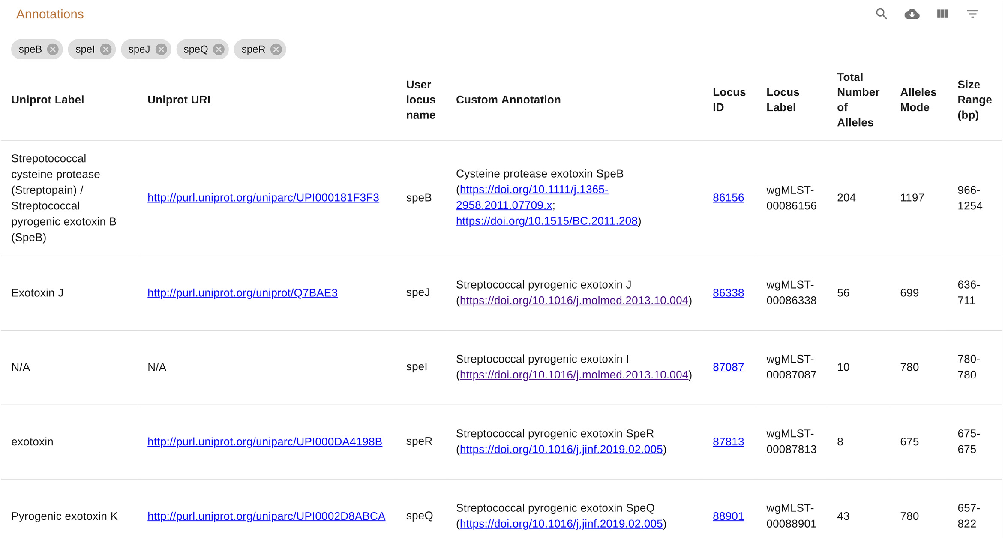
\includegraphics[width=\textwidth]{figures/chapter 3/Figure4.pdf}
    \caption[Schema loci table: search functionality.]{Schema loci table: search functionality. The figure presents the results of filtering for \textit{speB}, \textit{speI}, \textit{speJ}, \textit{speQ} and \textit{speR} in the \textit{user locus name} field of the \textit{Streptococcus pyogenes} schema 1. Note that the user provided annotations complement and correct some of the annotations retrieved from UniProt.}
    \label{fig:chap3_figure4}
\end{figure*}

\section{Discussion} \label{sec:ch3_discussion}

\ac{Chewie-NS} accomplishes four important goals. First, it stores all the information required to define a chewBBACA schema, facilitating accessibility of schemas so that different schemas can be easily compared and evaluated. Second, it maintains a public compendium of the variability in each locus. Since chewBBACA loci are \acp{ORF}, this will allow monitoring the variability of the proteins potentially encoded by these loci. This is important when studying microbial pathogens because small variations in sequence can lead to dramatic changes in virulence \cite{li_genome-wide_2019} or antimicrobial resistance \cite{van_der_linden_heterogeneity_2020}. On the other hand, allelic diversity can also be indicative of stabilizing or diversifying selective pressures, which in turn can be leveraged to obtain insights into pathogen evolution or interaction with the host \cite{yamaguchi_identification_2019}. Allelic diversity is also important in reverse vaccinology \cite{moxon_editorial_2019} and to monitor the continued potential efficacy of some available vaccines \cite{maiden_impact_2018}. Third, through its integration with chewBBACA, it offers a simplified way for the user to control the flow of information between the local instance and \ac{Chewie-NS}. This is important to keep the local instance of chewBBACA updated with the current common nomenclature stored in \ac{Chewie-NS} databases and to contribute new alleles to the common databases, but it also allows for limited sharing of data to comply with any regulations the user may be operating under. Finally, the proposed workflow hopes to stimulate and facilitate data sharing between users using the same schemas, allowing for a faster detection of strain similarity, therefore contributing for genomic epidemiology studies and also faster outbreak detection and investigation by expediting strain comparison between different laboratories or institutions. Although the current integration of chewBBACA with \ac{Chewie-NS} facilitates the user interaction with \ac{Chewie-NS} when using this allele-calling software, the \ac{API} can be exploited by other allele-calling software to also interact directly with \ac{Chewie-NS}, allowing an easier submission of schemas and of new alleles to schemas not created with chewBBACA. 

The definition of a \ac{wg/cgMLST} schema involves not only the choice of the target loci and of what constitutes a locus (for instance, an \ac{ORF} as defined by Prodigal \cite{hyatt_prodigal_2010} in the case of chewBBACA, or a fragment of \ac{DNA} between two primers in traditional \ac{MLST}), but also the algorithm and parameters of the allele-calling software. If one uses the same set of target loci defined in the same way, but a different allele-calling software, one cannot guarantee that the alleles called for a given isolate would be the same as with another allele-calling software, a problem that can potentially become all the more acute with the identification of novel alleles. Even when using the same allele-calling software, if the parameters used are different, the alleles identified in a given isolate may also be different. Moreover, the addition of novel alleles to a schema that do not conform with the parameters defined initially may have hard to anticipate consequences on the subsequent allele-calling processes. Upstream of this, we would like to stress the importance of the use of shared assembly pipelines, to ensure that the deposited allele sequences are determined based on standardized procedures, as it has been shown that different assemblers can result in different variants in the assembly \cite{firtina_apollo_2020} and that this variability can introduce artificial allelic variability, even when using the same schema and allele-calling software.

The possibility of setting up local instances of \ac{Chewie-NS} in a simplified way using Docker Compose facilitates creating private services that can cater to trusted groups of users and allow the implementation of \ac{Chewie-NS} in institutions operating under strict privacy rules. In a public health context, this can also be used to deploy services allowing an easier communication between different agencies operating under distinct mandates.

The databases currently available in the public instance of \ac{Chewie-NS} (\url{https://chewbbaca.online/}) include schemas developed within the INNUENDO project \cite{llarena_innuendo_2018} for \textit{Salmonella enterica}, \textit{Campylobacter jejuni}, \textit{Escherichia coli} and \textit{Yersinia enterocolitica}, a schema developed for \textit{Arcobacter butzleri} \cite{isidro_virulence_2020}, an adaptation of a schema generated using the Ridom SeqSphere+ software for \textit{Acinetobacter baumannii} \cite{higgins_development_2017} and in-house developed schemas for \textit{Streptococcus agalactiae} and \textit{Streptococcus pyogenes}. However, we expect that users of chewBBACA and of other allele-calling software will increasingly contribute schemas for these as well as additional species to be deposited in \ac{Chewie-NS}.

\section{Data Availability} \label{sec:ch3_data_availability}

\ac{Chewie-NS} is freely accessible at \url{https://chewbbaca.online/}. Its source code is hosted at \url{https://github.com/B-UMMI/Chewie-NS} together with instructions on how to deploy it locally using Docker Compose and the documentation can be found at \url{https://chewie-ns.readthedocs.io/}. A tutorial version of the server, which allows users to perform mock submissions of schemas and synchronizations with a much reduced database, can be accessed at \url{https://tutorial.chewbbaca.online/}.

\section{Acknowledgements} \label{sec:ch3_data_acknowledgements}

The authors would like to thank Catarina Inês Mendes for fruitful discussions and for her multiple design suggestions and Ana Correia for her guidance in solving issues with the \ac{Chewie-NS} implementation.

\section{Funding} \label{sec:ch3_data_funding}

Fundos Europeus Estruturais e de Investimento (FEEI) and Fundação para a Ciência e a Tecnologia (\ac{FCT}) [LISBOA-01-0145-FEDER-016417]; FCT and FEDER [01/SAICT/2016 no. 022153]; FCT [PTDC/CCI-BIO/29676/2017]. Funding for open access charge: FEEI and FCT [LISBOA-01-0145-FEDER-016417]. \\
Conflict of interest statement. None declared.


%-----------------------------------------------------------------
% Paper 3 - GAS wgMLST schema
%------------------------------------------------------------------
\newpage
\thispagestyle{empty}
\chapter{Annotated Whole-Genome Multilocus Sequence Typing Schema for Scalable High-Resolution Typing of \textit{Streptococcus pyogenes}\label{ch:paper3}}
\thispagestyle{empty}
\cleardoublepage
\mbox{}\\
\vspace{8cm}

This chapter is a reproduction of the following publication:

A. Friães, R. Mamede, M. Ferreira, J. Melo-Cristino, M. Ramirez, Annotated Whole-Genome Multilocus Sequence Typing Schema for Scalable High-Resolution Typing of \textit{Streptococcus pyogenes}, Journal of Clinical Microbiology, Volume 60, Issue 6, May 2022. DOI: \url{https://doi.org/10.1128/jcm.00315-22}

The supplementary information referred throughout the text can be consulted in this chapter before the section of references. 

DENV represents a public health threat and economic burden in affected countries. The risk of exposure to DENV is increasing, not only because of travel to endemic regions but also due to the broader dissemination of the mosquito vector, making the burden of dengue very significant. 

The availability of genomic data is key to understanding viral evolution and dynamics and supporting improved control strategies. Currently, the use of second-generation sequencing technologies, which can be applied both directly to patient samples (shotgun metagenomics) and to PCR-amplified viral sequences (amplicon sequencing), is the most informative approach to monitor viral dissemination and genetic diversity by providing, in a single methodological step, identification and characterization of the whole viral genome at the nucleotide level. This makes DENV identification and characterization through genomic analysis by developing software where the lessons learned in Chapters \ref{ch:paper1} and \ref{ch:paper2} are applied.

We have developed DEN-IM, a one-stop, user-friendly, containerised and reproducible workflow for the analysis of Dengue virus short-read sequencing data from both amplicon and shotgun metagenomics approaches. DEN-IM was designed to perform a comprehensive analysis in order to generate either assemblies or consensus of full DENV coding sequences and to identify their serotype and genotype. DEN-IM can also detect all four DENV serotypes and the respective genotypes present in a spiked sample, raising the possibility that DEN-IM can play a role in the identification of co-infection cases whose prevalence is increasingly perceived in highly endemic areas. 

My contribution to this publication included the design, implementation and optimisation of the DEN-IM workflow, including the creation of  the Docker containers for all dependencies. Two databases, one comprising 3830 DENV sequences for the retrieval of the reads of interest from the input samples, and a second comprising 161 sequences representing the genetic diversity of all DENV sero and genotypes were constructed by me.  Additionally, I've also written the manuscript.

\cleardoublepage 

\begin{center}
\large
\textbf{Annotated Whole-Genome Multilocus Sequence Typing Schema for Scalable High-Resolution Typing of \textit{Streptococcus pyogenes}}
\end{center}

Ana Friães$^{1,*}$, 
Rafael Mamede$^{1,*}$, 
Mariana Ferreira$^1$,
José Melo-Cristino$^1$, 
Mário Ramirez$^1$,

$^1$Instituto de Microbiologia, Instituto de Medicina Molecular, Faculdade de Medicina, Universidade de Lisboa, Lisboa, Portugal 

$^*$Contributed equally

\section{Abstract}

\textit{Streptococcus pyogenes} is a major human pathogen with high genetic diversity, largely created by recombination and horizontal gene transfer, making it difficult to use \ac{SNP}-based genome-wide analyses for surveillance. Using a \ac{GbG} approach on 208 complete genomes of \textit{S. pyogenes}, a novel \ac{wgMLST} schema was developed, comprising 3,044 target loci. The schema was used for \ac{cgMLST} analyses of previously published data sets and 265 newly sequenced draft genomes with other molecular and phenotypic typing data. Clustering based on \ac{cgMLST} data supported the genetic heterogeneity of many \textit{emm} types and correlated poorly with \ac{PFGE} macrorestriction profiling, superantigen gene profiling, and \ac{MLST} sequence type, highlighting the limitations of older typing methods. While 763 loci were present in all isolates of a data set representative of \textit{S. pyogenes} genetic diversity, the proposed schema allows scalable \ac{cgMLST} analysis, which can include more loci for an increased resolution when typing closely related isolates. The \ac{cgMLST} and \ac{PopPUNK} clusters were broadly consistent in this diverse population. The \ac{cgMLST} analyses presented results comparable to those of \ac{SNP}-based methods in the identification of two recently emerged sublineages of \textit{emm1} and \textit{emm89} and the clarification of the genetic relatedness among isolates recovered in outbreak contexts. The schema was thoroughly annotated and made publicly available on the \ac{Chewie-NS} online platform (\url{https://chewbbaca.online/species/1/schemas/1}), providing a framework for high-resolution typing and analyzing the genetic variability of loci of particular biological interest.

\section{Introduction}

\textit{Streptococcus pyogenes} (\ac{GAS}) remains a significant cause of global morbidity and ranks among the top 10 infectious causes of death \cite{carapetis_global_2005}. In 2018, the \ac{WHO} highlighted the importance of developing a \ac{GAS} vaccine and set out priority activities to reach this goal, including a better characterization of the epidemiology of \ac{GAS} infections and the identification of appropriate candidate antigens \cite{vekemans_path_2019}.

In recent decades, sequence-based typing of the hypervariable region of the \textit{emm} gene, encoding the M protein, was the most frequently used method to identify \ac{GAS} lineages \cite{beall_sequencing_1996}. However, complementary methods have long been used, which, together with \textit{emm} typing, allow finer discrimination of the circulating strains, including serotyping of the major backbone pilus protein (T antigen), \ac{PFGE} macrorestriction profiling, \ac{MLST}, and profiling of superantigen (SAg)-coding genes \cite{carrico_illustration_2006, friaes_superantigen_2013, enright_multilocus_2001}.

\ac{WGS} analysis allowed the identification of emerging intra-\textit{emm} clones with increased fitness or virulence that were otherwise indistinguishable by other typing methods. Such is the case of \textit{emm}89 clade 3, which emerged during the 2000s and quickly outcompeted other emm89 lineages \cite{friaes_emergence_2015, turner_emergence_2015, zhu_molecular_2015}. Isolates from this lineage lack the genes encoding hyaluronic acid capsule biosynthesis and carry a high-expression promoter in the operon encoding streptolysin O and NAD-glycohydrolase (Pnga-3) \cite{turner_emergence_2015, zhu_trading_2015}. More recently, an \textit{emm}1 lineage ($M1_{UK}$), differing from the contemporary globally disseminated \textit{emm}1 lineage ($M1_{global}$) by 27 \ac{SNPs}, was identified in the United Kingdom \cite{lynskey_emergence_2019-1} and subsequently reported in The Netherlands, the United States, and Canada \cite{rumke_dominance_2020, li_m1uk_2020, demczuk_identification_2019}.

\ac{WGS} has been decisive in clarifying the molecular and evolutionary mechanisms underlying the success of long-term-circulating lineages \cite{nasser_evolutionary_2014, beres_molecular_2010} and has proven useful in the identification of outbreak-related cases \cite{turner_community_2017, coelho_genomic_2019}. Genomic data have the additional potential benefit of providing information on the variability of candidate vaccine antigens and genes involved in antimicrobial resistance \cite{davies_atlas_2019, beres_integrative_2022}, further supporting the use of \ac{HTS} in \ac{GAS} surveillance.

Most genome-wide analyses performed on \ac{GAS} have been based on the comparison of \ac{SNPs} between isolates. This usually involves mapping short-read sequence data or aligning de novo-assembled sequences to a selected reference genome \cite{turner_emergence_2015, zhu_molecular_2015, zhu_trading_2015, lynskey_emergence_2019, nasser_evolutionary_2014, beres_molecular_2010, turner_community_2017, coelho_genomic_2019, davies_atlas_2019}. However, the choice of an appropriate reference is challenging when simultaneously comparing diverse lineages \cite{maiden_mlst_2013, neumann_core_2019}, such as in population-based studies of \textit{S. pyogenes} infection isolates. \ac{SNP}-based phylogenetic analysis also requires the removal of regions of recombination, which are an important source of diversity in \ac{GAS} \cite{davies_atlas_2019, maiden_mlst_2013, neumann_core_2019, mcgregor_multilocus_2004}. These limitations can be largely overcome by the use of \ac{GbG} approaches like \ac{wgMLST} or \ac{cgMLST} \cite{carrico_primer_2018}, which do not require comparison to a reference genome and which intrinsically dampen the effect of recombination \cite{maiden_mlst_2013, neumann_core_2019, leopold_bacterial_2014}. \ac{MST} (MST)-like downstream analyses further facilitate the use of \ac{wg/cgMLST}. Additionally, \ac{wg/cgMLST} schemas can be curated and maintained in centralized databases, providing a standardized nomenclature and ensuring reproducibility and comparison of results across laboratories \cite{maiden_mlst_2013, carrico_primer_2018, higgins_development_2017, bletz_defining_2018}. Indeed, similarly to \ac{SNP}-based approaches, \ac{cgMLST} schemas have been successfully used for both outbreak identification and population-based surveillance of multiple pathogens \cite{neumann_core_2019, leopold_bacterial_2014, higgins_development_2017, bletz_defining_2018, abdel-glil_whole-genome-based_2021, pinto_insights_2019, bardenstein_brucellosis_2021}. However, it is important to remember that \ac{wg/cgMLST} is not designed to interrogate noncoding regions of the genome and therefore would have been unable to detect the polymorphisms in the \textit{nga-ifs-slo} promoter present now in the $M1_{global}$ lineage \cite{lynskey_emergence_2019}.

The aims of this study were to define a publicly available annotated \ac{wgMLST} schema for \textit{S. pyogenes} and evaluate its suitability for high-resolution typing and documenting the variability of loci encoding proteins of biological relevance.

\section{Materials and Methods}

\textbf{Bacterial strains and data sets}. A collection of 265 nonduplicate \ac{GAS} strains isolated from pharyngitis, skin and soft tissue infections, and normally sterile sites in Portugal between 2001 and 2009 was selected for \ac{HTS} and comparison of \ac{cgMLST} with other typing methods (see supplemental Data Set 1 in reference \cite{friaes_supplemental_2023}). These isolates were previously characterized regarding \textit{emm} type, T type, \ac{PFGE} profile, SAg gene profile, and antimicrobial resistance \cite{friaes_superantigen_2013, friaes_group_2012, pato_streptococcus_2018, friaes_changes_2013, noauthor_emstreptococcus_nodate} and represent four \textit{emm} types: \textit{emm}1, \textit{emm}3, \textit{emm}4 (including erythromycin-resistant and -susceptible isolates), and \textit{emm}89 (including isolates carrying P\textit{nga}-1, P\textit{nga}-2, and P\textit{nga}-3) \cite{friaes_emergence_2015}.

In order to evaluate the performance of the proposed \ac{wgMLST} schema in more diverse collections, outbreak recognition, and the identification of recently emerged intra-\textit{emm} lineages of interest, publicly available data sets from three previous publications were also included \cite{lynskey_emergence_2019, coelho_genomic_2019, davies_atlas_2019}. Data Set 2 comprises 2,006 assemblies from a collection of isolates previously selected to represent the genetic, geographic, temporal, and clinical diversity of \ac{GAS} \cite{davies_atlas_2019}. Data Set 3 consists of 119 isolates associated with 21 outbreaks recorded in England from 2010 to 2015 and 170 contemporaneous sporadic isolates with the same \textit{emm} types \cite{coelho_genomic_2019}. Data Set 4 comprises 135 assemblies from noninvasive \textit{emm}1 isolates recovered in the United Kingdom from 2009 to 2016 \cite{lynskey_emergence_2019} and the MGAS5005 complete genome that was used as a reference. The United Kingdom assemblies include 123 isolates carrying 27 \ac{SNPs} characteristic of the recently emerged $M1_{UK}$ lineage and 5 intermediate isolates carrying 13 or 23 of those \ac{SNPs} \cite{lynskey_emergence_2019}. Data Set 5 includes all the \textit{emm}89 assemblies included in Data Sets 1 to 4 (\textit{n} = 194) and the 7 complete genomes of \textit{emm}89 that were used to create the schema.

The majority of the strains included in Data Sets 2 to 4 \cite{friaes_supplemental_2023} were retrieved from collections of publicly available genome assemblies \cite{blackwell_exploring_2021, oleary_reference_2016}. For strains for which it was not possible to retrieve a public genome assembly, the raw sequencing data were downloaded from the \ac{ENA} and subsequently assembled. All assemblies were filtered according to assembly quality, \textit{emm} type, and multilocus \ac{ST} criteria, as detailed below.

\textbf{High-throughput sequencing}. Genomic DNA was extracted from cultures of \ac{GAS} grown overnight in Todd-Hewitt broth (Oxoid, Basingstoke, UK) using the PureLink genomic DNA minikit (Invitrogen, Carlsbad, CA, USA). The initial bacterial lysis step was carried out in the presence of 45 U of mutanolysin (Sigma-Aldrich, St. Louis, MO, USA) and 86 $\mu$g of hyaluronidase (Sigma-Aldrich, St. Louis, MO, USA). \ac{WGS} libraries were generated using the Nextera DNA library preparation kit (Illumina, San Diego, CA, USA). The libraries were sequenced in an Illumina MiSeq or NextSeq instrument.

\textbf{Sequencing data analysis}. Raw sequence reads were assembled with INNUca v4.2.2 \cite{noauthor_release_nodate}, with the following parameters: \textit{-s Streptococcus pyogenes}, \textit{-g 2}, \textit{–estimatedMinimumCoverage 10}, \textit{–trueCoverageProceed}, and \textit{–fastQCproceed}. Samples that failed any of the quality control steps related to sequence quality or assembly coverage were excluded from the data sets. Assemblies are available as supplemental material \cite{friaes_supplemental_2023}.

\textit{In silico} \ac{ST} prediction was performed using MLST v2.19.0 \cite{seemann_mlst_nodate} with default parameters and the PubMLST database updated on 11 March 2021. Genome assemblies with partial matches to any of the \ac{MLST} genes or for which it was not possible to identify at least one of the \ac{MLST} genes were excluded, except for ST293, ST403, ST404, and ST688, which lack the \textit{yqiL} gene, and ST1087, which lacks the \textit{xpt} gene. Strains with a predicted \ac{ST} that was inconsistent with the classification reported in the original study were also excluded.

The \textit{emm} type was determined using emmTyper v0.2.0 \cite{noauthor_release_nodate-2} with verbose mode and the \ac{CDC} M-type-specific sequence databases updated on 11 March 2021. Genome assemblies without an identified \textit{emm} type, with matches only for alleles flagged in the \ac{CDC} database as possible \textit{emm}-like genes, or with a predicted \textit{emm} type that was inconsistent with the classification reported in the original study were excluded from the data sets. Assemblies classified with multiple \textit{emm} types were also excluded (multiple subtypes of the same \textit{emm} type were accepted), except for \textit{emm}34/\textit{emm}230 (\textit{emm}34 corresponds to the \textit{enn} gene, and the \textit{emm} type is 230), \textit{emm}13L/\textit{emm}13 (these two types correspond to the same sequence), and other cases that were inspected in Geneious v8.1.9 to validate matches to the \textit{emm} gene.

Variant calling to determine the set of \ac{SNPs} in each assembled genome from Data Set 4 \cite{friaes_supplemental_2023} was performed with Snippy v4.6.0 \cite{noauthor_release_nodate-3} with default parameters and the complete genome of strain MGAS5005 (RefSeq accession no. \texttt{GCF\_000011765.3}) as the reference strain.

The \textit{Pnga} variant was determined with SeqTyper v2.3 \cite{noauthor_b-ummiseq_typing_2025} with default parameters. A Fasta file with the sequences for all variants was given as the input to the blast module, followed by variant calling with the assembly module.

\textbf{Schema creation, annotation, and curation}. The complete genomes available in the \ac{NCBI} RefSeq database as of 20 July 2020 were downloaded to select a set of 208 genome assemblies (see Table S1 in the supplemental material) \cite{friaes_supplemental_2023} for schema creation with chewBBACA v2.7.0 \cite{silva_chewbbaca_2018}. Assemblies with a status of suppressed in the \ac{NCBI} database were excluded, except for accession no. \texttt{GCF\_001535505.1}, \texttt{GCF\_001547815.1}, \texttt{GCF\_000013525.1}, and \texttt{GCF\_900636425.1}, whose status was changed to suppressed after the schema creation and allele-calling processes. Loci originating from these four genomes were inspected to ensure their validity. This initial schema seed, composed of 3,318 distinct loci, was populated through the inclusion of allelic variants from all assemblies included in the data sets and sourced from public databases \cite{blackwell_exploring_2021, oleary_reference_2016}. For schema annotation, the chewBBACA UniprotFinder process and custom scripts \cite{noauthor_release_nodate-4} were used to create a file with locus coordinates and annotation terms selected from the UniProt database, prioritizing the selection of terms from Swiss-Prot over terms from TrEMBL, and from matches against the translated coding sequences in the GenBank files of the genomes used for schema creation. Some product and gene names were further complemented with relevant literature references. The annotated schema was thoroughly curated to identify and remove spurious loci such as gene fusions, truncated genes, and paralogous loci. These loci were identified based on the retrieved annotations, the inspection of the genomic context, and the list of paralogous loci reported by the chewBBACA AlleleCall process and a custom script evaluating interlocus similarity \cite{noauthor_release_nodate-4}. Due to the minimum sequence length parameter enforced during schema creation, the \textit{sagA} gene, present in the streptolysin S-encoding operon, was not in the initial schema. Given the importance of this gene for \ac{GAS} pathogenesis and the potential interest in its variability, a locus was added representing the \textit{sagA} gene. The full list of changes applied to the schema is available in Table S2 \cite{friaes_supplemental_2023}.

The schema was uploaded to \ac{Chewie-NS} \cite{mamede_chewie_2021}, where a more detailed description of schema creation, annotation, and curation can be found (\url{https://chewbbaca.online/species/1/schemas/1}).

\textbf{cgMLST analysis}. Allelic profiles of the core loci (shared by 100\% of the isolates under analysis [cgMLST-100]) were used to create \ac{MST}s with the goeBURST algorithm in the desktop or online version of PHYLOViZ \cite{nascimento_phyloviz_2017, ribeiro-goncalves_phyloviz_2016}. Groups of isolates linked by up to \textit{n} different loci in the \ac{MST} were determined using the desktop version. The genes present in 95\% (cgMLST-95), 99\% (cgMLST-99), and 100\% (cgMLST-100) of the isolates were identified with the chewBBACA ExtractCgMLST process for Data Set 2. The lists of genes for each gene presence threshold are available as supplemental material \cite{friaes_supplemental_2023}. Intracluster and intercluster pairwise distances were determined using custom scripts \cite{noauthor_release_nodate-4}.

\textbf{PFGE cluster definition}. Previously generated SmaI/Cfr9I macrorestriction PFGE patterns \cite{friaes_superantigen_2013, friaes_group_2012, blackwell_exploring_2021, noauthor_emstreptococcus_nodate} were used to create a \ac{UPGMA} dendrogram with BioNumerics software (Applied Maths, Sint-Martens-Latem, Belgium). The Dice similarity coefficient was used, with optimization and position tolerance settings of 1.0 and 1.5, respectively. \ac{PFGE} clusters were defined based on $\geq80\%$ relatedness on the dendrogram \cite{carrico_illustration_2006}.

\textbf{Statistical analysis}. The results of cgMLST-100 and other typing methods were compared using \ac{SID}, the \ac{AW} coefficient, and the \ac{AR} coefficient \cite{carrico_illustration_2006, severiano_adjusted_2011}, calculated with an online tool (\url{http://www.comparingpartitions.info/}). For comparison with other typing methods, groups were defined by cutting \ac{MST}s at a suitable allelic difference to have an \ac{SID} similar to that of the method to which it was being compared.

\textbf{Data availability}. The annotated \ac{wgMLST} schema and a detailed description of its development are publicly available in \ac{Chewie-NS} \cite{mamede_chewie_2021} at \url{https://chewbbaca.online/species/1/schemas/1}. The genome assemblies and allele-calling results for each data set, a static version of the \ac{wgMLST} schema, the list of loci in each subschema, the pairwise distances computed for Data Sets 2 and 3, and Tables S1, S2, S5, and S9 can be found in the supplemental material \cite{friaes_supplemental_2023}. Raw sequencing data and sample metadata for the 265 isolates included in Data Set 1 have been deposited in the \ac{ENA} under project accession number PRJEB49967. The custom scripts used for schema annotation, curation, and result analyses are part of the Schema Refinery repository \cite{noauthor_release_nodate-4}.

\section{Results}

\textbf{Development of the wgMLST schema for \textit{S. pyogenes}}. The final annotated \ac{wgMLST} schema comprises 3,044 loci with 371,549 alleles. Out of these, 1,096 (36\%) loci presented low variability, presenting 1 to 19 \ac{DNA} alleles (see Fig. S1 in the supplemental material). These correspond essentially to genes that were identified in a minority of assemblies, mostly associated with prophages and other mobile genetic elements. The exception is \textit{sagA}, encoding the streptolysin S precursor peptide, which presented only 13 alleles despite being ubiquitous among S. pyogenes isolates. The short length of this locus (162 \ac{bp}) may be partly responsible for the limited number of alleles.

On the opposite extreme, among the 10 most variable loci (>750 alleles) are genes encoding well-known surface-exposed virulence factors but also transcriptional regulators known to play a major role in \ac{GAS} pathogenesis and virulence, namely, CovS, RopB, and Mga. For these loci, the diversity of \ac{DNA} alleles also results in a very large number of protein variants (range, 535 to 1,695) (Fig. S2).

Specific analyses can be performed through the identification and creation of subschemas for smaller sets of biologically relevant loci, such as genes encoding virulence factors and transcriptional regulators, for which subschemas are provided as supplemental material \cite{friaes_supplemental_2023}.

\textbf{Comparison of cgMLST with other typing methods}. To compare \ac{cgMLST} analysis with conventional typing methods, a collection of 265 infection isolates with previous information on \textit{emm} type, \ac{ST}, T type, \ac{PFGE} profile, \ac{PCR} profile of 11 SAg genes, and antimicrobial resistance was used (see Data Set 1 in \cite{friaes_supplemental_2023}). This data set includes isolates of \textit{emm} types 1, 3, 4, and 89; 15 distinct STs; 6 T types (17 isolates were nontypeable); 19 SAg profiles; and 16 \ac{PFGE} clusters (Table 1).

\newpage
\begin{figure*}[h!]
    \centering
    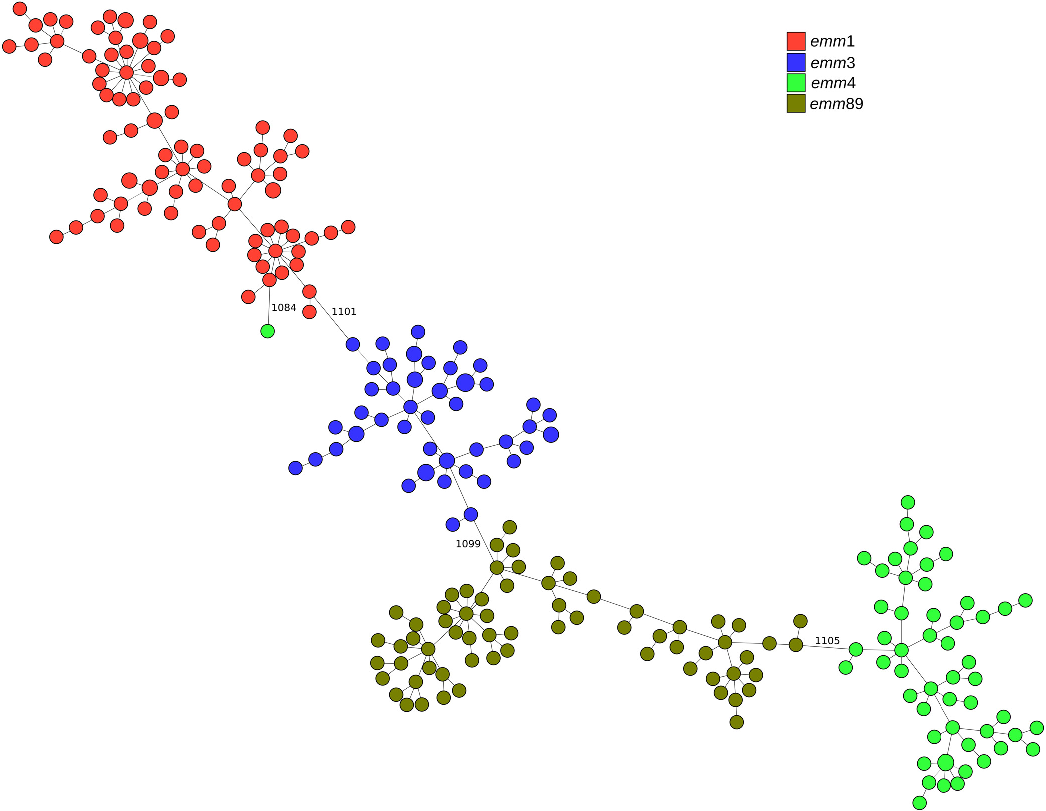
\includegraphics[width=\textwidth]{figures/chapter 4/Figure1.pdf}
    \caption{Minimum-spanning tree generated with the goeBURST algorithm for the cgMLST-100 profiles of 265 \text{S. pyogenes} isolates recovered in Portugal (see Data Set 1 in \cite{friaes_supplemental_2023}). The size of each node is proportional to the number of isolates with that particular cgMLST-100 profile on a logarithmic scale. Nodes are colored according to \textit{emm} type. Link distances of $\geq1,000$ allelic differences are labeled (from a total of 1,230 compared loci).}
    \label{fig:chap4_figure1}
\end{figure*}

Allele calling using the \ac{wgMLST} schema followed by cgMLST-100 analysis generated 245 different profiles representing 1,230 loci. The resulting \ac{MST} separated the isolates according to \textit{emm} type, except for one \textit{emm}4 isolate that did not cluster with the others (Fig. 1). The minimum distance between clusters of different \textit{emm} types varied between 1,084 and 1,105 allelic differences, while those among isolates of the same \textit{emm} type were $\leq28$ for \textit{emm}1, $\leq100$ for \textit{emm}3, $\leq157$ for \textit{emm}4 (excluding the distantly related isolate), and $\leq225$ for \textit{emm}89. Clustering of isolates at a cutoff of 1,000 differences created four groups separating the four \textit{emm} types and one singleton, corresponding to the \textit{emm}4 isolate, resulting in high concordance between the \ac{MST} groups linked by up to 1,000 different loci and \textit{emm} types (Table 1; see also Tables S3 and S4 in the supplemental material).

A lower congruence was obtained between the distributions of isolates in the \ac{MST} and the remaining typing methods (\ac{ST}, \ac{PFGE}, SAg profiling, and T type) (Fig. S3 to S6). The \ac{AW} and \ac{AR} values between T types and \ac{MST} groups linked by up to 1,000 different loci were only slightly lower than those of \textit{emm} types (Tables S3 and S4), but T type had a lower typeability since 17 isolates were nontypeable. Although MST groups linked by up to 45 different loci resulted in a number of partitions and \ac{SID}s comparable to those of \ac{ST}, SAg profiling, and \ac{PFGE} (Table 1), the \ac{AW} coefficient between \ac{MST} groups linked by up to 45 different loci and these typing methods was lower than that between \ac{MST} groups linked by up to 1,000 different loci and \textit{emm} type (Table S4). This means that \ac{MST} groups linked by up to 45 different loci could not confidently predict the \ac{ST}, \ac{PFGE} cluster, or SAg profile, or the converse, which was also reflected in lower \ac{AR} values (<0.900) (Table S3).

The use of a \ac{wgMLST} schema instead of a universally defined cgMLST-100 set of loci allows scalable analysis in which higher resolution can be obtained by including larger numbers of common loci when analyzing closely related isolates. As an example, the cgMLST-100 obtained exclusively for the \textit{emm}4 isolates grouped into the same \ac{MST} group linked by up to 1,000 different loci (\textit{n} = 54) comprises 52 profiles of 1,382 cgMLST-100 loci. The \textit{emm}4 isolates presenting the M phenotype of macrolide resistance (erythromycin resistant and clindamycin susceptible) shared ST39 and an SAg profile with most susceptible isolates (see Data Set 1 in \cite{friaes_supplemental_2023}), rendering these two methods unable to differentiate macrolide-resistant isolates. One \ac{PFGE} cluster was associated with macrolide resistance \cite{silva-costa_differences_2012}, although it also included two susceptible isolates. Similarly, one of the \ac{MST} groups linked by up to 33 different loci comprised exclusively all but two of the macrolide-resistant isolates (Fig. S7). Not surprisingly, the set of 46 loci that were present universally and exclusively in the subset of erythromycin-resistant isolates (list available in the supplemental material in reference 31) represents mostly phage-related genes, including \textit{mef}(A) and \textit{msr}(D), the genes most commonly associated with the M phenotype in \ac{GAS} \cite{silva-costa_macrolide-resistant_2015, iannelli_type_2018}.

\textbf{Performance of the wgMLST schema on a large and genetically diverse data set}. The genetic structure of the \ac{GAS} population is known to vary temporally and geographically, with an associated impact on the disease spectrum and incidence \cite{steer_global_2009, barnett_fall_2018}. To evaluate the performance of the proposed \ac{wgMLST} schema on the analysis of genetically diverse data sets, we used a large collection of isolates previously selected to represent the genetic, geographic, temporal, and clinical diversity of \ac{GAS} \cite{davies_atlas_2019}. A total of 2,006 assemblies were included in the data set, comprising 140 \textit{emm} types and 443 \ac{ST}s and organized into 292 phylogroups defined by \ac{PopPUNK} \cite{davies_atlas_2019, lees_fast_2019} (see Data Set 2 in \cite{friaes_supplemental_2023}).

We defined 1,321-locus cgMLST-95, 1,204-locus cgMLST-99, and 763-locus cgMLST- 100 schemas (available in the supplemental material in \cite{friaes_supplemental_2023}).

Allele call results identified 1,700 cgMLST-100 profiles. The resulting \ac{MST} indicates that many \textit{emm} types include diverse genetic lineages, with 12 of the 19 most prevalent \textit{emm} types (>30 isolates) comprising isolates distributed in multiple tree regions (Fig. 2). Accordingly, 50 of the 67 \textit{emm} types comprising $\geq10$ isolates included assemblies that differed in >50\% of the 763 cgMLST-100 loci (up to 708 differences [93\%] in \textit{emm}4) (Fig. 3A). In 31 of these \textit{emm} types, the mean intra-\textit{emm} allelic difference was larger than the smaller difference from another \textit{emm} type (Table S5). This is possibly due to the diversity of geographic and temporal origins of the isolates in this data set and is in line with a previous report of genetic heterogeneity within \textit{emm} types \cite{davies_atlas_2019}. It is also reflected in a low congruence between \textit{emm} types and \textit{MST} groups linked by up to 450 different loci despite similar \ac{SID} values (Tables S6 to S8).

\begin{landscape}
\vspace*{\fill}
\begin{figure*}[h!]
    \centering
    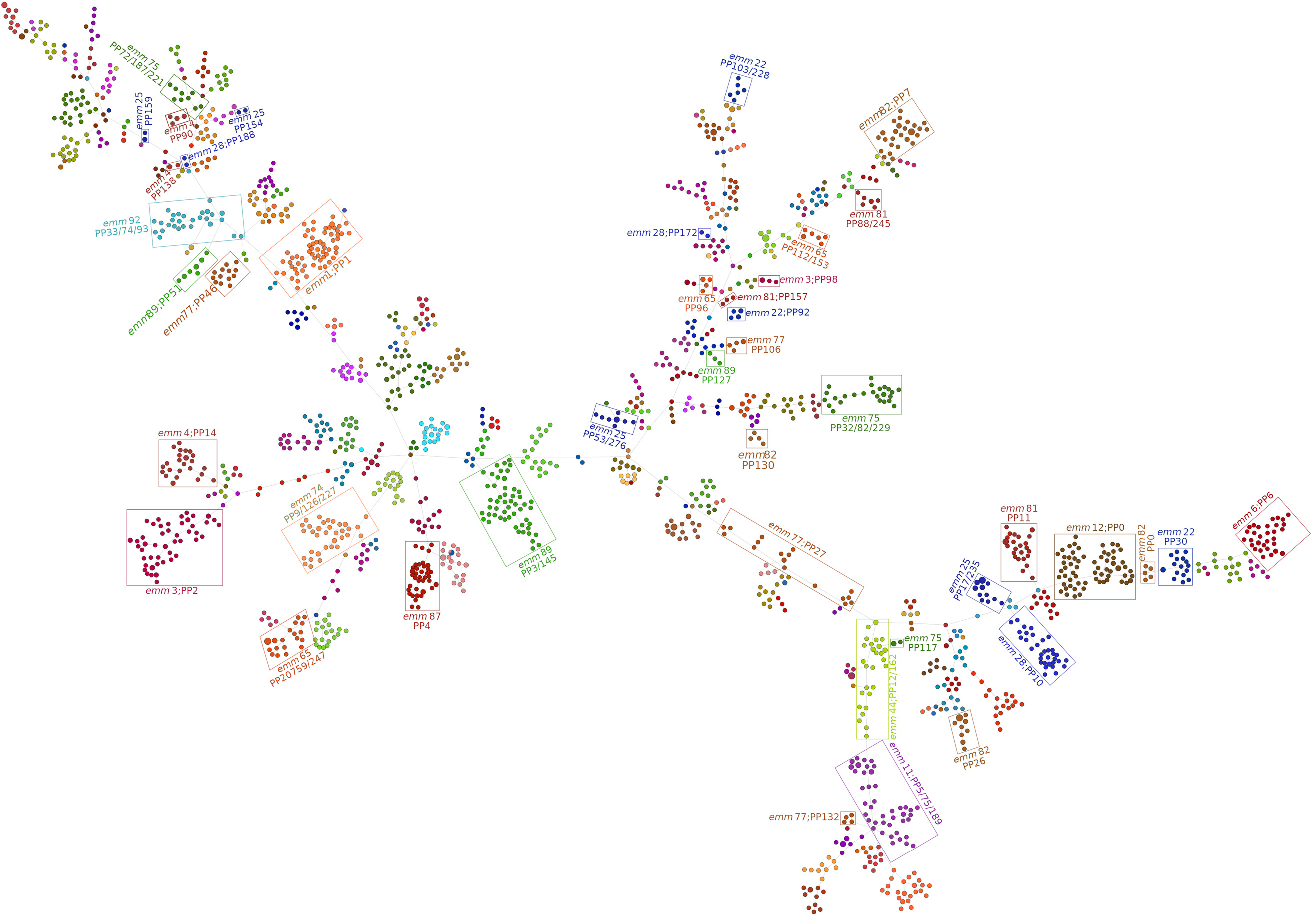
\includegraphics[height=0.9\textheight]{figures/chapter 4/Figure2.pdf}
    \caption{Minimum-spanning tree generated with the goeBURST algorithm for the \ac{cgMLST} profiles of 2,006 genetically diverse \textit{S. pyogenes} isolates recovered worldwide \cite{davies_atlas_2019} (see Data Set 2 in reference \cite{friaes_supplemental_2023}). The size of each node is proportional to the number of isolates with that particular \ac{cgMLST} profile on a logarithmic scale. Nodes are colored according to \textit{emm} type. Groups of clustered \textit{emm} types represented by >30 isolates are highlighted inside rectangles and labeled with the respective \textit{emm} types and PopPUNK phylogroup numbers (for simplicity, isolated nodes of \textit{emm} types 4, 22, 44, 65, 75, 77, 81, and 92 are not highlighted). A total of 763 core loci were compared.}
    \label{fig:chap4_figure2}
\end{figure*}
\vspace*{\fill}
\end{landscape}

\newpage
\begin{figure*}[h!]
    \centering
    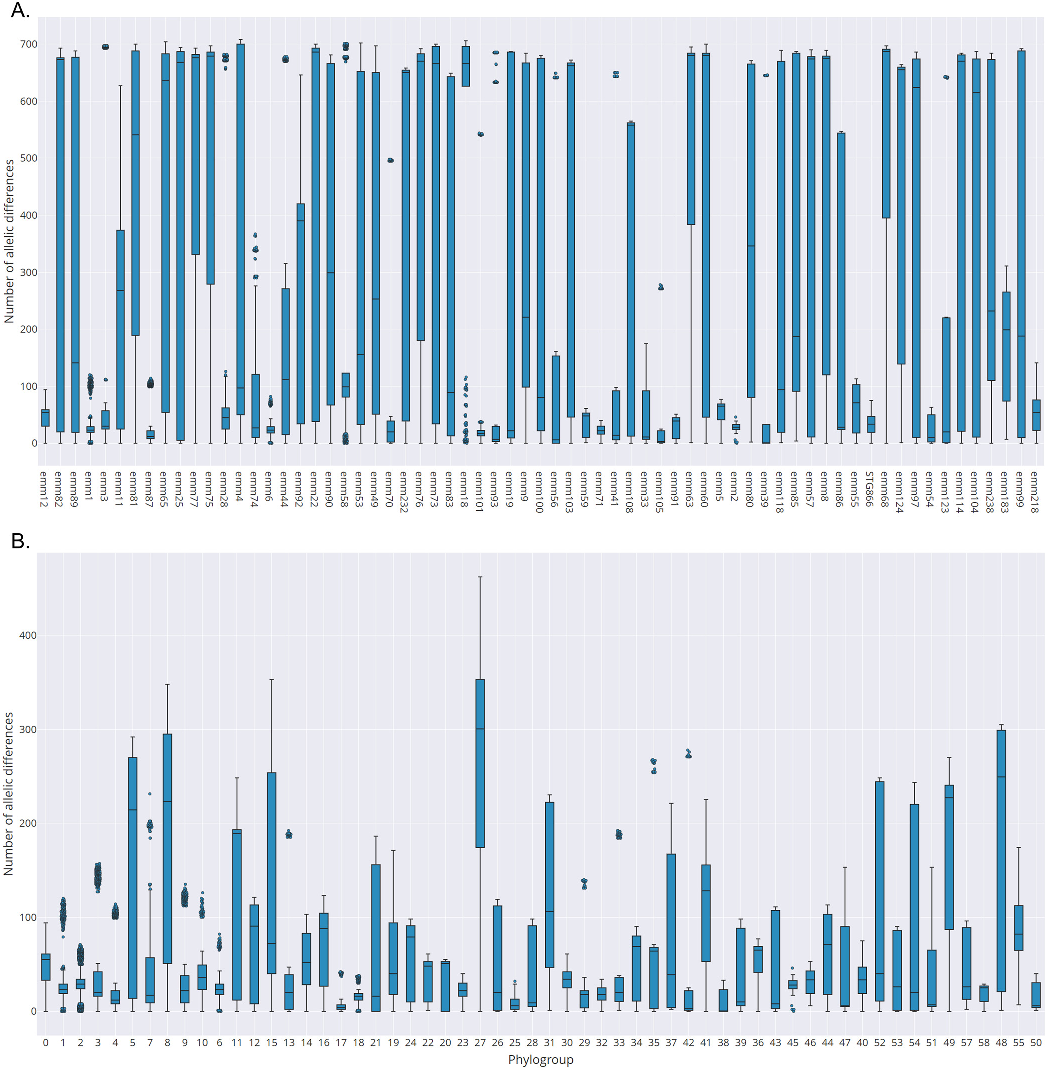
\includegraphics[width=\textwidth]{figures/chapter 4/Figure3.pdf}
    \caption{Box-and-whisker plots for the pairwise distances of the assemblies from Data Set 2 \cite{davies_atlas_2019, friaes_supplemental_2023} included in each \textit{emm} type with $\geq10$ isolates (A) or in each PopPUNK phylogroup with $\geq10$ isolates (B). The distances were calculated based on the allele call results for the 763 cgMLST-100 loci of the 2,006 assemblies (interactive versions of these plots are available as supplemental material in reference \cite{friaes_supplemental_2023}).}
    \label{fig:chap4_figure3}
\end{figure*}

The overall congruence between \ac{ST}s and \ac{MST} groups linked by up to 50 different loci was poor although slightly higher than that observed for the less diverse Data Set 1 (\ac{AR} coefficients of 0.810 and 0.709, respectively) (Table S7). In contrast, there was good congruence, with high \ac{AW} and \ac{AR} values, between \ac{PopPUNK} phylogroups and \ac{MST} groups linked by up to 200 different loci (Tables S7 and S8). Still, \ac{PopPUNK} phylogroups can be rather diverse, including multiple \ac{ST}s and isolates differing in up to 61\% of the core 763 loci (phylogroup 27) (Fig. 3B; Table S9), highlighting the advantage of using multiple methods for analyzing the evolution of \ac{GAS} lineages.

\textbf{Performance of the wgMLST schema in an outbreak context}. To evaluate the potential contribution of the proposed \ac{wgMLST} schema for outbreak recognition, we used a previously published data set comprising isolates from 21 outbreaks in England and contemporaneous nonrelated isolates with the same \textit{emm} types \cite{coelho_genomic_2019}. A total of 119 outbreak isolates and 170 sporadic isolates were included (see Data Set 3 in \cite{friaes_supplemental_2023}). Allele calling for the 119 outbreak isolates identified 58 profiles of 1,263 cgMLST-100 loci. In agreement with the \ac{SNP}-based clustering presented previously \cite{coelho_genomic_2019}, the \ac{MST} clustered the isolates according to \textit{emm} type, with a minimum distance of 1,079 allelic differences between isolates of different \textit{emm} types, while isolates of different subtypes or outbreaks of the same \textit{emm} type were more closely related (Fig. 4). Individual \textit{MST}s were created for \textit{emm} types 1, 5, 11, 28, 75, 89, and 94, including outbreak and sporadic isolates (Fig. S8 to S14). Since these \ac{MST}s included only isolates sharing the same \textit{emm} type, they comprised larger sets of cgMLST-100 loci (1,384 to 1,547 loci), potentially allowing higher resolution in the discrimination of outbreak isolates. Ten isolates with epidemiological links could be excluded from the respective outbreaks because they did not cluster with isolates of the same outbreak or differed by too many loci (Table S10 and Fig. S8 and S11 to S13). These isolates also matched the outbreak exclusion
criteria based on \ac{SNP} analysis (18). Except for these 10 excluded isolates, outbreak isolates linked in the \ac{MST}s shared >99.5\% of their core genome (maximum link distance of 6 allelic differences), and the mean distance within a given outbreak was much lower than the mean distance among sporadic isolates of the same \textit{emm} type (Table 2). However, in \textit{emm} types 1 and 5, there were sporadic isolates with \ac{cgMLST} profiles very similar to those of outbreak 1 (OB1) and OB19, respectively (0 to 2 allelic differences), indicating that these outbreak strains were also present in the community (Table 2; Fig. S8 and S9).

\begin{figure*}[h!]
    \centering
    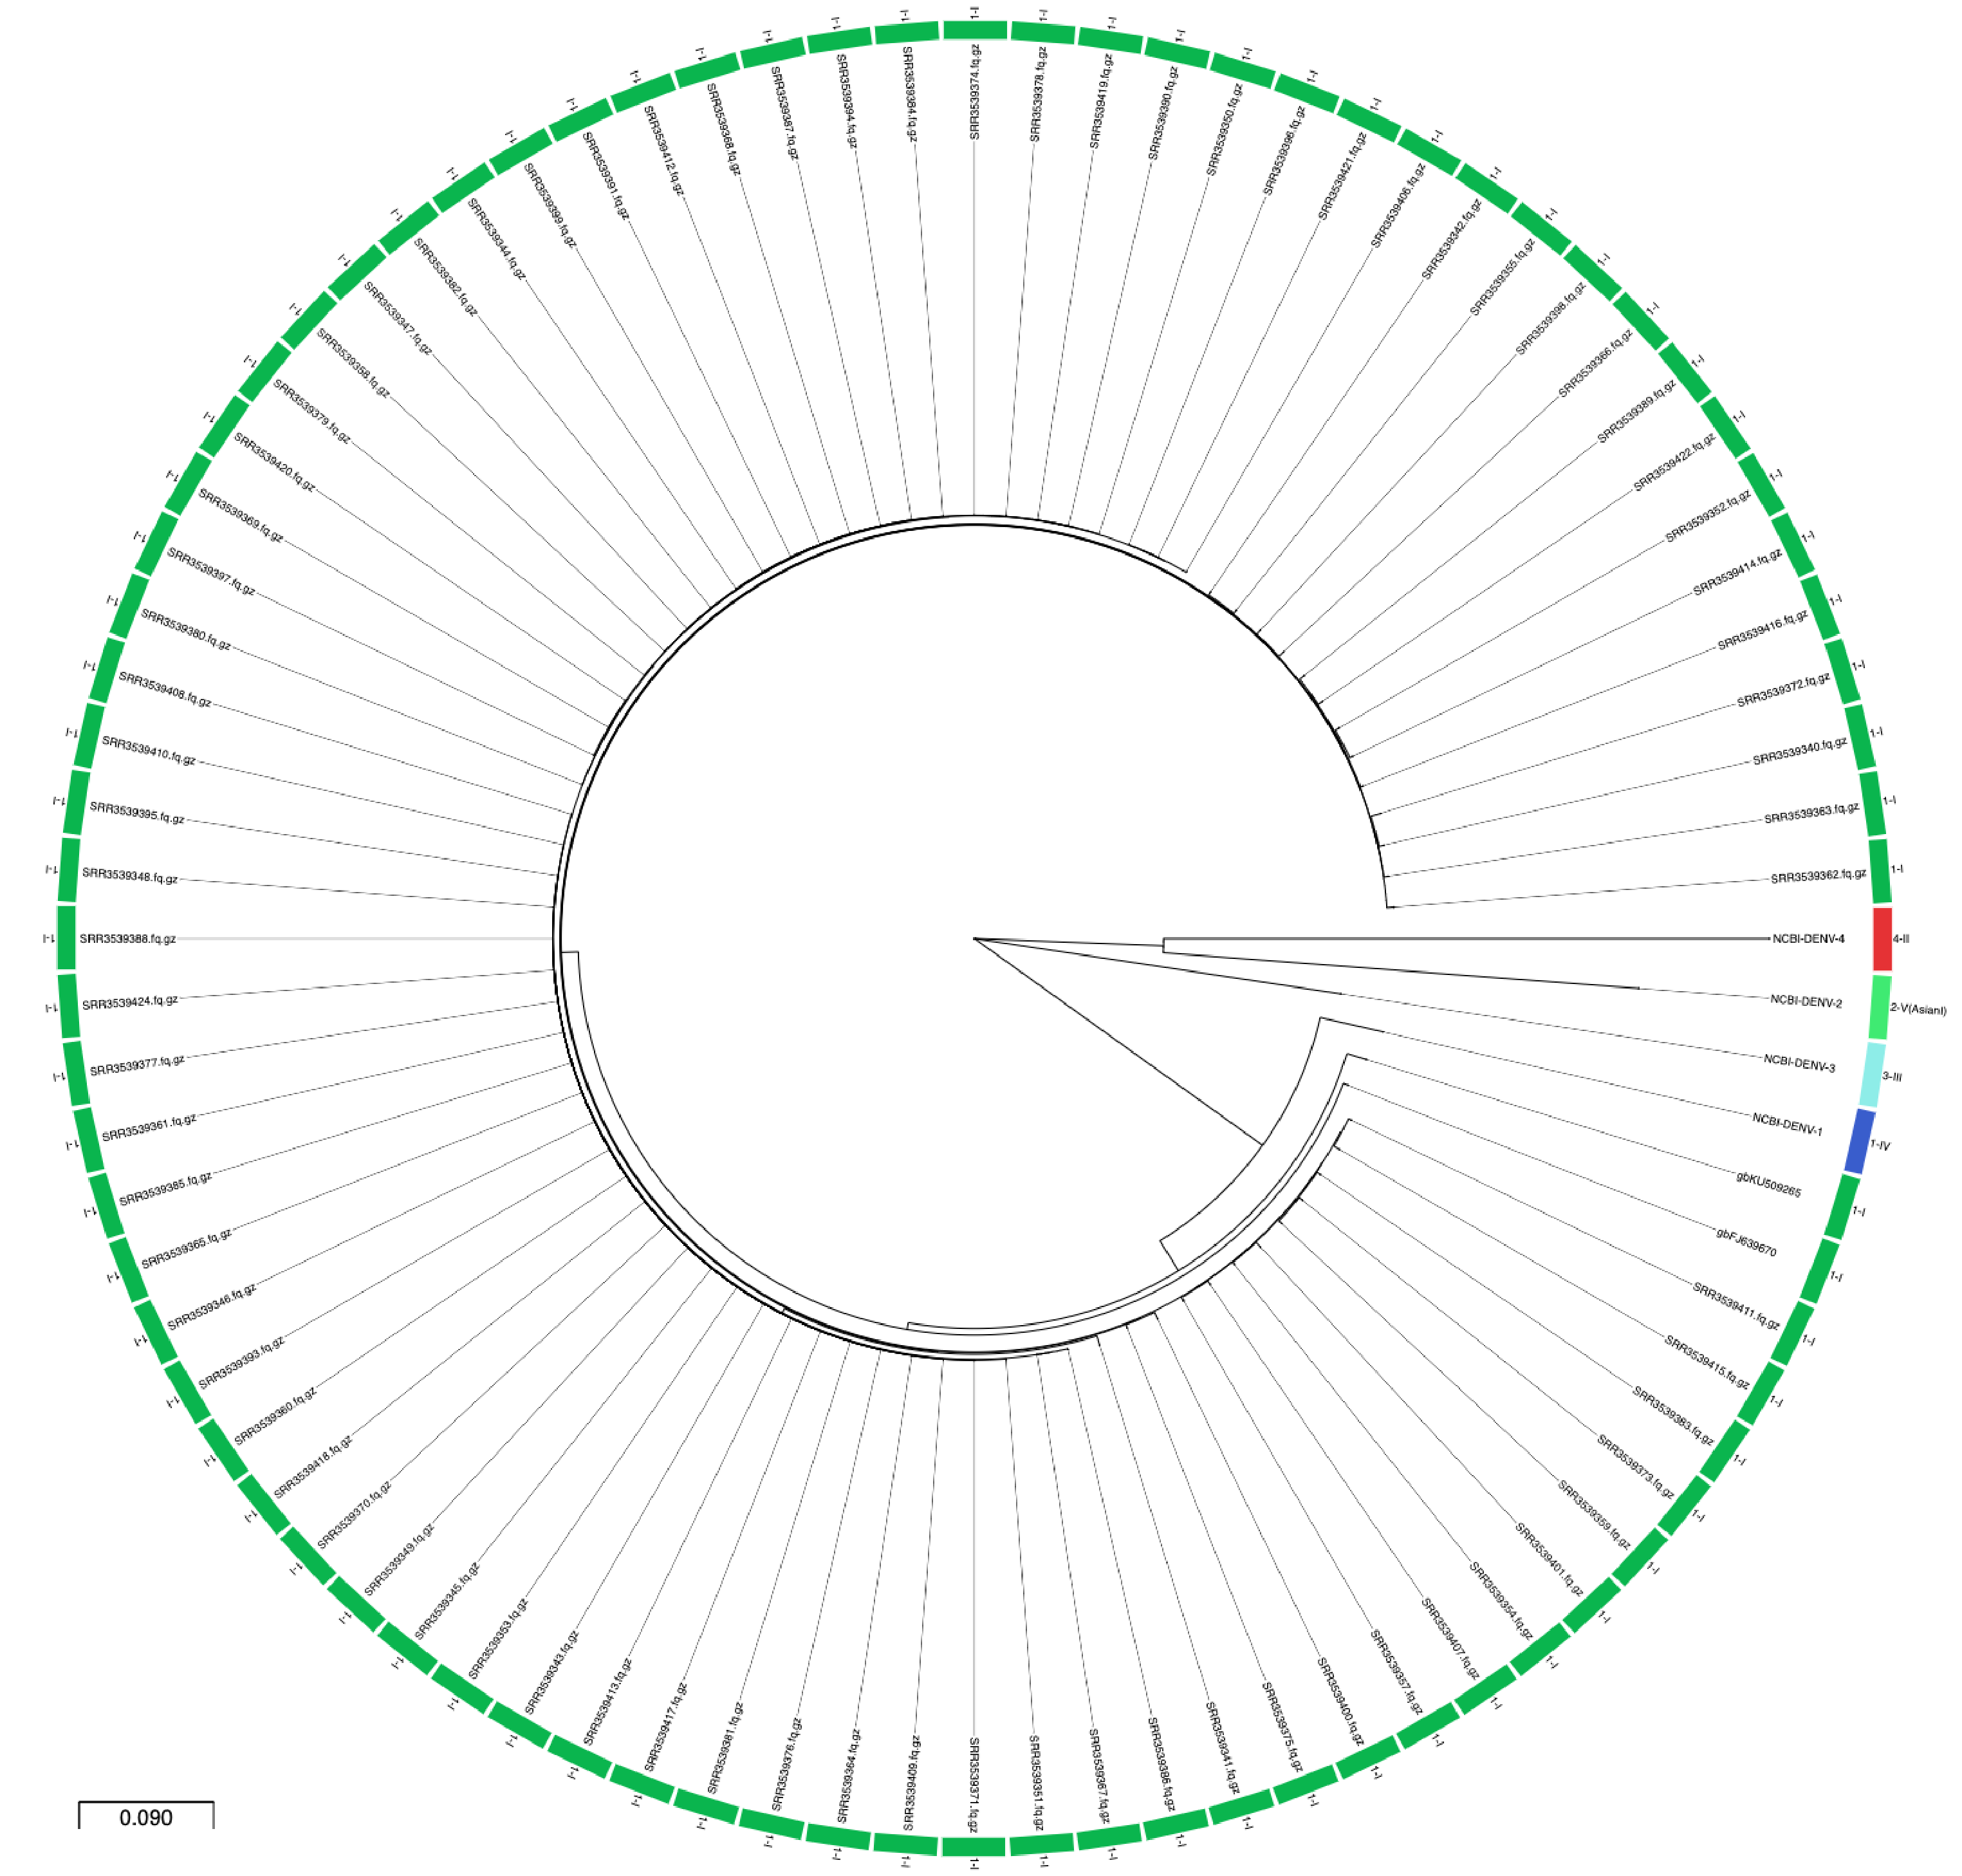
\includegraphics[width=\textwidth]{figures/chapter 4/Figure4.pdf}
    \caption{Minimum-spanning tree generated with the goeBURST algorithm for the cgMLST-100 profiles of 119 outbreak \textit{S. pyogenes} isolates recovered in the United Kingdom \cite{coelho_genomic_2019} (see Data Set 3 in reference \cite{friaes_supplemental_2023}). The size of each node is proportional to the number of isolates with that particular \ac{cgMLST} profile on a logarithmic scale. The nodes are colored according to the \textit{emm} type, and the outer ring is colored according to the outbreak number. Link distances are labeled as the number of allelic differences between nodes (from a total of 1,263 compared loci).}
    \label{fig:chap4_figure4}
\end{figure*}

\textbf{Performance of the wgMLST schema in the identification of recently emerged lineages}. We tested if the proposed \ac{wgMLST} schema has enough discriminatory power to identify two recently emerged intra-\textit{emm} lineages that were originally identified by whole-genome \ac{SNP} analysis, namely, $M1_{UK}$ and \textit{emm}89 clade 3 \cite{turner_emergence_2015, zhu_molecular_2015, lynskey_emergence_2019}. Allele calling was performed for the 135 assemblies from noninvasive \textit{emm}1 isolates \cite{lynskey_emergence_2019} together with the complete genome of strain MGAS5005, a reference representative of the $M1_{global}$ lineage (see Data Set 4 in \cite{friaes_supplemental_2023}). The graph in Fig. 5 represents the resulting \ac{MST} with all links of up to 19 differences depicted. All $M1_{UK}$ isolates were tightly clustered, together with an intermediate isolate ($M1_{inter}$) carrying 23 of the 27 \ac{SNP}s characteristic of the $M1_{UK}$ lineage \cite{lynskey_emergence_2019}. The \ac{MST} links within this cluster ranged between 0 and 13 differences, while the closest links to the $M1_{inter}$ cluster (13 \ac{SNP}s) and an $M1_{global}$ isolate were 20 and 31 differences, respectively. $M1_{global}$ isolates presented higher genomic diversity, with \ac{MST} links of up to 49 differences. Allele calling was performed for all \textit{emm}89 assemblies included in the four data sets described above and all the complete \textit{emm}89 genomes used to create the schema (\textit{n} = 201) (see Data Set 5 in \cite{friaes_supplemental_2023}). In addition, the P\textit{nga} variant was determined for all isolates. The absence of the \textit{hasA} gene of the capsule locus was confirmed in all P\textit{nga}-3 isolates, while all other isolates carried this gene, except for two ST568 isolates that have an internal nonsense codon in \textit{hasA}. The graph depicting all links of up to 55 differences (Fig. 6) showed limited diversity in the isolates carrying P\textit{nga}-3, which clustered closely, with \ac{MST} links with 0 to 27 differences, while the shortest link to a P\textit{nga}-2 isolate was 57 differences. The P\textit{nga}-2 and, especially, P\textit{nga}-1 isolates were more diverse, presenting fewer links with up to 55 differences and comprising multiple sublineages associated with different \ac{ST}s (Fig. 6; Fig. S15). Both the wider geographic range and collection time span may contribute to this higher diversity. As previously reported \cite{friaes_emergence_2015}, \ac{MLST} was not suitable for discriminating P\textit{nga}-3 isolates from those carrying P\textit{nga}-2 since ST101 was prevalent among both lineages (Fig. S15). Analysis of the \textit{emm}89 isolates from Data Set 1 showed that P\textit{nga}-3 isolates and most P\textit{nga}-2 isolates were also grouped into the same \ac{PFGE} cluster, and some of them shared the same SAg profile, while the T serotype B3264 was ubiquitous, except for the single P\textit{nga}-1 isolate (T11) and one P\textit{nga}-3 isolate that was nontypeable (Fig. S16 to S18). \ac{PopPUNK} clustering also could not discriminate P\textit{nga}-3 isolates, which were clustered with isolates carrying P\textit{nga}-1 and P\textit{nga}-2 in phylogroup 3 (see Data Set 5 in \cite{friaes_supplemental_2023}).

\section{Discussion}

The reduced costs of \ac{HTS} have facilitated a wider application of whole-genome data to the epidemiological surveillance of multiple pathogens. This leads to a requirement for standardized analysis pipelines producing reproducible and portable results that can be easily compared across laboratories and with those of previously used typing methods \cite{sabat_overview_2013}. Here, we propose a \ac{wgMLST} schema for \textit{S. pyogenes}, consisting of 3,044 loci. Hard-defined \ac{cgMLST} schemas comprising the subsets of loci present in 95\% (1,321 loci), 99\% (1,204 loci), and 100\% (763 loci) of the assemblies of a collection representing the genetic diversity of \textit{S. pyogenes} (19) are also presented.

\begin{figure*}[h!]
    \centering
    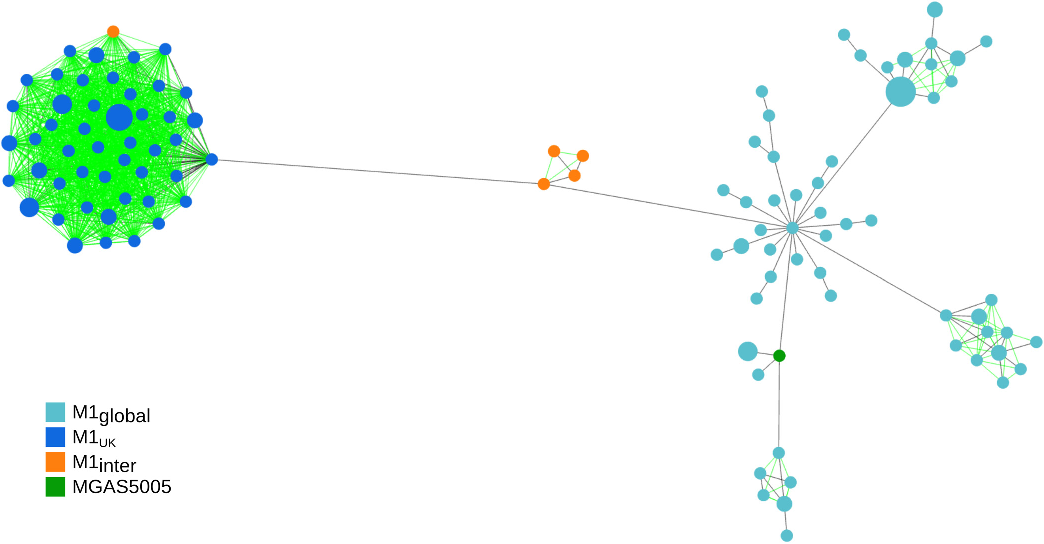
\includegraphics[width=\textwidth]{figures/chapter 4/Figure5.pdf}
    \caption{Graph representation of the relationships between the cgMLST-100 profiles of 135 noninvasive \textit{emm}1 isolates recovered in the United Kingdom \cite{lynskey_emergence_2019} and reference strain MGAS5005 (see Data Set 4 in reference \cite{friaes_supplemental_2023}), depicting all links with $\leq19$ allelic differences (from a total of 1,404 compared loci). The size of each node is proportional to the number of isolates with that particular cgMLST-100 profile on a logarithmic scale. Nodes are colored according to the M1 lineage, with MGAS5005 (reference genome for the $M1_{global}$ lineage) in green. Links that would not be present in the standard \ac{MST} are shown in green. Links shown in black represent the \ac{MST} links and may represent distances with >19 allelic differences.}
    \label{fig:chap4_figure5}
\end{figure*}

However, the use of a \ac{wgMLST} schema from which the \ac{cgMLST} loci are selected according to the specific data set under analysis has the advantage of allowing the inclusion of larger subsets of loci and, hence, increased resolution when comparing closely related isolates \cite{maiden_mlst_2013}. This can be particularly important to track the emergence of intra-\textit{emm}-type sublineages or identify outbreak-related isolates. The application of the schema proposed here to previously published data sets and analysis of the resulting \ac{MST}s showed a performance comparable to that of \textit{SNP}-based methods in distinguishing recently emerged intra-\textit{emm}-type sublineages as well as in identifying clusters of epidemiologically and genetically related isolates associated with local, short-term outbreaks \cite{turner_emergence_2015, lynskey_emergence_2019, coelho_genomic_2019}. Analyses based on \ac{wg/cgMLST} build upon the strengths of \ac{GbG} approaches, which do not require a reference genome or the removal of regions of recombination \cite{maiden_mlst_2013, neumann_core_2019, leopold_bacterial_2014}. This is particularly important when analyzing collections of genetically diverse lineages, such as in long-term surveillance studies, particularly in organisms where mobile genetic elements and recombination play major roles in genomic plasticity and evolution, such as \textit{S. pyogenes} \cite{davies_atlas_2019, mcgregor_multilocus_2004}. Moreover, \ac{GbG} approaches constitute a framework that has been widely used in surveillance, which can facilitate the transition to \ac{wg/cgMLST} by reference laboratories involved in surveillance activities. Comparison of \ac{cgMLST}-based clustering with other typing methods used for \textit{S. pyogenes} revealed poor concordance, although in temporally and geographically restricted data sets, the groups defined by \textit{emm} typing were also supported by \ac{cgMLST}. By including a much higher number of loci, \ac{cgMLST} was expected to present a higher discriminatory power than the traditional seven-gene \ac{MLST} schema and to further discriminate isolates sharing the same \ac{ST} \cite{neumann_core_2019, bletz_defining_2018}. However, such a simplistic expectation was not universally borne out by the data, which highlights the limitations of the seven-gene \ac{MLST} schema to correctly identify \ac{GAS} lineages based on broader genomic information. It is worth noting that from the seven genes included in traditional \ac{MLST}, two (\textit{gtr} and \textit{yqiL}) were excluded from the \ac{wgMLST} schema because they shared alleles with paralogous genes, and one (\textit{xpt}) was absent in at least one \ac{GAS} lineage and therefore was not always included in the \ac{cgMLST} analysis. In contrast, a good correlation was found between \ac{cgMLST} clustering and \ac{PopPUNK} \cite{davies_atlas_2019, lees_fast_2019}, another whole-genome-based clustering method. However, the flexibility of \ac{wg/cgMLST} allows increased resolution by lowering the number of allelic differences used to define clusters and a dynamic \ac{cgMLST} definition, providing further discrimination within \ac{PopPUNK} clusters. The proposed \ac{wgMLST} schema is publicly available on the \ac{Chewie-NS} platform \cite{mamede_chewie_2021}, where multiple statistics regarding the whole schema and individual loci can be visualized (\url{https://chewbbaca.online/species/1/schemas/1}).

\begin{figure*}[h!]
    \centering
    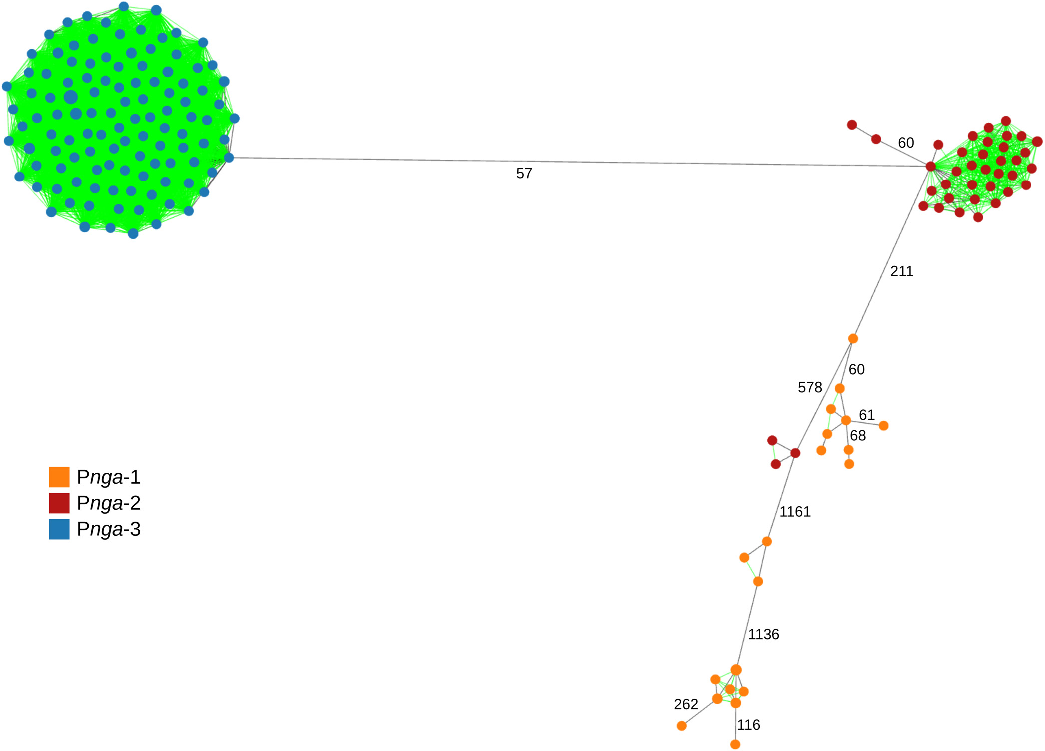
\includegraphics[width=\textwidth]{figures/chapter 4/Figure6.pdf}
    \caption{Graph representation of the relationships between the cgMLST-100 profiles of 201 \textit{emm}89 isolates (see Data Set 5 in reference \cite{friaes_supplemental_2023}) depicting all links with $\leq55$ allelic differences (from a total of 1,279 compared loci). The size of each node is proportional to the number of isolates with that particular cgMLST-100 profile on a logarithmic scale. Nodes are colored according to the variant of the \textit{nga} promoter (P\textit{nga}). Links that would not be present in the standard \ac{MST} are shown in green. Links shown in black represent the \ac{MST} links and may represent distances with >55 allelic differences (labeled links).}
    \label{fig:chap4_figure6}
\end{figure*}

The close integration with the chewBBACA suite \cite{silva_chewbbaca_2018} facilitates its use in surveillance and epidemiological studies and the maintenance of a common nomenclature across different studies. By virtue of the comprehensive annotation, the database can be used to obtain relevant data for basic research, such as the variability of genes of interest (virulence factors, antimicrobial resistance genes, candidate vaccine antigens, and transcriptional regulators, etc.) \cite{davies_atlas_2019, beres_integrative_2022} in addition to its use for typing purposes.

\section{Acknowledgments}

R.M. was supported by the \ac{FCT} (grant 2020.08493.BD). Partial support was received from the ONEIDA project (LISBOA-01-0145-FEDER-016417), cofunded by the FEEI (Fundos Europeus Estruturais e de Investimento) from the Programa Operacional Regional de Lisboa, Portugal, 2020 (POR Lisboa 2020), and by national funds from the \ac{FCT} and the LISBOA-01-0145-FEDER-007391 project, cofunded by FEDER through POR Lisboa 2020 and the \ac{FCT}.

\newpage

\section{Supplemental Material}




%-----------------------------------------------------------------
% Discussion
%-----------------------------------------------------------------
\newpage
\thispagestyle{empty}
\chapter{General Discussion \label{ch:discussion}}
\thispagestyle{empty}
\cleardoublepage
\renewcommand*{\thefootnote}{\arabic{footnote}}

\mbox{}\\
\vspace{8cm}

\section{A brief note on software development practices}

I start this discussion by mentioning a subject that tends to be overlooked in bioinformatics: good practices in software development. After the initial thrill of coming up with a concept for a tool and implementing a rudimentary proof-of-concept, it is time to tidy up. Developing bioinformatics software that is efficient, maintainable, and reliable is the shortest route to contribute to its wide adoption and long-term success \cite{jimenez_four_2017, coelho_for_2024, black_ten_2020}. The process and effort of writing well-structured and documented code can take up as much time as the algorithmic intricacies, but it is essential to ensure maintainability, especially in the long-term. While I think it is not necessary to follow each piece of advice given by Uncle Bob\footnote{\url{https://en.wikipedia.org/wiki/Robert_C._Martin}}, defining a handful of simple requirements for good code quality can help avoid turning something simple into a convoluted mess.

While working on chewBBACA 3 and Chewie-NS, presented in \textbf{\autoref{ch:paper1}} and \textbf{\autoref{ch:paper2}}, I aimed to maintain good code quality standards, as I knew that that could greatly influence long-term support. In chewBBACA 3, the compartmentalization of the code into multiple modules containing smaller functions played an important role in organizing the code to maximize reusability and maintainability. When evident, functions were added to modules based on more general categories, such as functions for file operations (reading and writing files), sequence manipulation and clustering (processing and clustering of DNA and protein sequences), and multiprocessing operations (functions to divide and process inputs in parallel to improve efficiency). Compartmentalization helped to keep track of the set of functions that I had already implemented, reducing the tendency to reimplement functions in distinct parts of the code, and providing a collection of reusable functions interconnecting the code and making the codebase more coherent.

When development stretches over long periods, as was the case for chewBBACA 3, often forgetful developers (!) or new contributors will have difficulty understanding the code if it is not well documented. That is why I included \textit{docstrings} in almost every function in chewBBACA 3 and added comments to code parts whose function may seem cryptic or when it is important to explain design choices. The code documentation made it easier to jump right into development and avoid adding redundant or code-breaking changes by better understanding what the code was doing and the parts that needed to be improved or expanded. From an end-user perspective, especially for non-technical users, usage documentation is more important than code documentation. A well-structured and well-written usage documentation helps users quickly understand how to start using software and explore its functionalities \cite{karimzadeh_top_2018}. In that regard, I co-created usage documentation for chewBBACA 3 and \ac{Chewie-NS}, with quick start guides, step-by-step tutorials, and detailed instructions about each module's functionalities or for the \ac{API} endpoints and \ac{UI} in the case of \ac{Chewie-NS}. For command line software such as chewBBACA 3 it is also important to provide clear usage documentation and relevant information about each step being executed and any warnings or errors that might be raised \cite{seemann_ten_2013}. I worked on adding clear and detailed help messages for chewBBACA's modules and on printing information about normal execution or warnings and errors to the command line to help users understand each step and help resolve any issues. However, I did not add the creation of a log file, which is an excellent way to save detailed information about the execution of the process for post-analysis and debugging. 

Providing clear instructions and multiple options for installation is also of utmost importance, as difficulties during software installation often discourage users from using it \cite{alser_packaging_2024}. In this regard, making software available through a package management system, such as \textit{conda}\footnote{\url{https://anaconda.org/anaconda/conda}} (for bioinformatics software, the Bioconda distribution channel \cite{gruning_bioconda_2018} is often used) or \textit{PyPI}\footnote{\url{https://pypi.org/}} for Python packages simplifies the installation process. chewBBACA 3 is available through both \textit{conda} and \textit{PyPI}, which allows users to install it quickly and painlessly, avoiding common installation issues, such as having to resolve conflicts between incompatible dependencies versions. Another common practice in bioinformatics is the use of containerization, provided by platforms such as Docker, to package and isolate software and their dependencies, ensuring portability and consistency of the results across platforms \cite{gruening_recommendations_2018, nust_ten_2020, boettiger_introduction_2015, kadri_containers_2022}. A Docker image for chewBBACA 3 is available\footnote{\url{https://hub.docker.com/repository/docker/ummidock/chewbbaca/general}} and the deployment and management of Chewie-NS instances is only possible through the orchestration of multiple Docker containers with Docker Compose\footnote{\url{https://docs.docker.com/compose/}}. Workflow managers, such as Nextflow\footnote{\url{https://www.nextflow.io/}} and Snakemake\footnote{\url{https://snakemake.readthedocs.io/en/stable/}}, further simplify software usage by helping users set up and automate tasks \cite{wratten_reproducible_2021, strozzi_scalable_2019}. Using a workflow manager to streamline analyses with chewBBACA 3 could further simplify and promote its usage, but it is something I did not have the opportunity to work on.

Another practice that promotes reproducibility and sustainability is software testing, as regularly testing the functionality of software, especially if automated, can help assess software performance and detect unexpected issues \cite{krafczyk_scientific_2019}. Testing is a critical, but underused, aspect of scientific software development that I and others have advocated in a publication \cite{van_der_putten_software_2022}. I implemented automated standard functionality testing for chewBBACA 3 to ensure that it produces the expected results and detect issues arising due to minor changes or the introduction of new functionalities. Ultimately, I think that learning and upholding good practices for software development is crucial to developing quality software and maximizing its applicability in the long-term, as well as being a valuable skill for any developer. For Pythonistas like me, it is worth it to once in a while open a Python console and type \textit{import this}\footnote{\url{https://peps.python.org/pep-0020/}}.

\section{Limitations of CDS prediction in wg/cgMLST}

Accurate \ac{CDS} prediction is of the utmost importance in \ac{wg/cgMLST}. This is generally done in one of two ways: by aligning reference alleles to genome assemblies to identify similar alleles based on parameters such as sequence identity and coverage \cite{jolley_open-access_2018}; or through \textit{ab initio} or model-based \ac{CDS} prediction tools that scan genome assemblies to identify \ac{ORFs} that are subsequently filtered to identify putative \ac{CDSs} \cite{dimonaco_no_2022}. Prodigal is a well-known \textit{ab initio} prokaryotic \ac{CDS} predictor that chewBBACA used up to version 3.3.0 \cite{hyatt_prodigal_2010, silva_chewbbaca_2018}. However, Prodigal has not been actively maintained, raising concerns about its long-term support. As part of the work developed in \textbf{\autoref{ch:paper1}} to improve chewBBACA, I substituted Prodigal by Pyrodigal \cite{larralde_pyrodigal_2022}. Pyrodigal provides Python bindings to Prodigal, improving the performance and offering greater control over the \ac{CDS} prediction process, while also ensuring results consistent with Prodigal's latest stable version\footnote{\url{https://github.com/hyattpd/Prodigal/releases/tag/v2.6.3}}. \textbf{\autoref{ch:paper1}} evaluated the performance of chewBBACA only at the module level. Benchmarking the key steps in each of chewBBACA's modules, especially if varying the number of \ac{CPU} cores used to better assess scalability, would have provided valuable information to understand which steps were most optimized and which still have room for improvement. Although the performance of the \ac{CDS} prediction step was not directly measured, it is safe to assume that Pyrodigal, which was optimized to reduce memory usage and runtime compared to Prodigal \cite{larralde_pyrodigal_2022}, contributed to the efficiency of chewBBACA 3 compared to its previous versions.

Although efficiency gains are definitely important, the true value of switching to Pyrodigal lies in having greater control over the \ac{CDS} prediction process. With Prodigal, \ac{CDS} prediction was only possible by calling Prodigal directly. In contrast, Pyrodigal provides Python bindings that enable finer control of the \ac{CDS} prediction parameters. This allowed to seamlessly integrate \ac{CDS} prediction into chewBBACA 3 and maintain results consistent with previous chewBBACA versions. Furthermore, this can be further explored to implement changes that may significantly improve the \ac{CDS} prediction process compared to what is presented in \textbf{\autoref{ch:paper1}}. Possible improvements include selecting from multiple file formats for the output file containing the \ac{CDS} prediction results, such as GenBank and translated \ac{CDSs}, which currently can only be written in FASTA format. In addition, the scores attributed to each \ac{CDS} can be accessed before writing the results, which, through a thorough validation process, may allow the definition of a score threshold used to exclude spurious \ac{CDSs} predicted by Pyrodigal, leading to improvements in allele calling and a reduction in the number of spurious loci included in the schema seeds created by the \textit{CreateSchema} module.

The prediction of spurious \ac{CDSs} is the main disadvantage of using a \textit{ab initio} or model-based \ac{CDS} predictor. The predicted \ac{CDSs} may not match any known gene, making validation difficult, or there may be a consistent deviation from reference alleles that have been experimentally validated, such as when the predicted \ac{CDSs} are in-frame but shorter than the reference alleles or are out of frame compared to reference alleles \cite{dimonaco_no_2022}. This may contrast with alignment-based \ac{CDS} prediction, used in \ac{wg/cgMLST} platforms such as \ac{BIGSdb}, which may predict less spurious \ac{CDSs} due to the use of more conservative parameters, but will have a limited capacity to identify more divergent alleles or \ac{CDSs} corresponding to genes not in the reference database. The discrepancies between both \ac{CDS} prediction strategies hinder reproducibility. wg/cgMLST schemas and results generated with chewBBACA 3 will not be directly comparable and may lead to different conclusions than the results generated on a platform that uses an alignment-based \ac{CDS} predictor. Adding alignment-based CDS prediction to chewBBACA 3 can help complement Pyrodigal results, while also allowing users to define parameters that approximate those used by other \ac{wg/cgMLST} platforms, promoting interoperability and further adoption of chewBBACA 3. In fact, a combinatory approach is already used in some genome annotation pipelines, such as Prokka, Bakta, and PGAP, to improve \ac{CDS} prediction and annotation \cite{seemann_prokka_2014, schwengers_bakta_2021, li_refseq_2021}. Adopting a similar strategy in chewBBACA 3, especially if also defining a threshold based on the scores computed by Pyrodigal to filter out potential spurious \ac{CDSs}, would definitely improve \ac{CDS} prediction and, consequently, the accuracy of the results. Validating the results produced by this strategy would require a thorough evaluation with reference datasets for both experimentally validated and spurious \ac{CDSs}, which could prove to be a laborious process, but would certainly help establish a framework for more accurate \ac{CDS} prediction, especially in \ac{wg/cgMLST}.

\section{Advantages and disadvantages of hash-based allele identification}

The high \ac{ANI} values between the genomes of the species datasets used to evaluate chewBBACA 3 in \textbf{Chapter \ref{ch:paper1}} reflect the composition of the public databases from where the genomes were sourced \cite{oleary_reference_2016, blackwell_exploring_2021}. Through the analysis of datasets used in other studies and testing datasets created to evaluate chewBBACA's performance, I observed that, for most species, the degree of inter-species similarity in available genome collections was also high, on average. This observation is supported by multiple studies that indicate \% ANI as the average for species-level...(CITE SOME ANI PAPER!). Genomes with highly similar sequences may share a significant fraction of identical \ac{CDSs}. Thus, using alignment to compare loci in a wg/cgMLST schema with genomes in a pairwise fashion can be inefficient and redundant if the process keeps identifying the same \ac{CDSs}.

The first published version of chewBBACA already determined if the \ac{CDSs} predicted from the input genomes were in the schema without using alignment, but would do this for every single genome, even if the same \ac{CDS} was found in all genomes. To further optimize the exact matching process, I decided to implement a deduplication step after the gene prediction step. This deduplication step identifies the set of distinct \ac{CDSs} identified in all input genomes, returning a hash table with \ac{CDS} SHA-256 hashes as keys and the list of genomes containing each \ac{CDS} as values. The SHA-256 hashes are used as unique identifiers for the exact matching between the \ac{CDSs} and the schema allele hashes, and are shorter than the actual \ac{CDS} sequences, which reduces memory usage compared to using the sequences as keys. Associating the list of genomes with a \ac{CDS} to the \ac{CDS} SHA-256 hash allows identifying and classifying all genomes with a particular \ac{CDS}, avoiding redundant comparisons. An issue that I identified while testing \ac{CDS} deduplication with large datasets was that the lists of genome string identifiers associated to each key could contain many values and occupy a lot of memory, which meant that storing the hash table in memory could become impractical for systems without a lot of \ac{RAM}. Mapping the genome string identifiers to unique integer identifiers and using lists of integer identifiers as values reduced memory usage but was not enough to drop memory usage to the range of values adequate for most users to be able to perform large-scale analysis. To further reduce memory usage, I used modified polyline encoding (CITE NUMCOMPRESS) to compress the lists of genome integer identifiers, yielding strings that occupy less memory than the original lists, and allowing large-scale analysis with the memory available in most modern laptops, as reported in Chapter \ref{ch:paper1} and testing during development.

Although implementing a solution for exact matching that integrates sequence deduplication, sequence hashing, and modified polyline encoding is more complex than simply comparing the CDSs identified in each genome against a \ac{wg/cgMLST} schema, the gains in efficiency far outweigh the increase in complexity since it allows chewBBACA to be used at a scale that was not previously possible.

One possible limitation of this approach is that it assumes that the CDSs identified in larger genome collections are highly repeated. This is in part true for single-species datasets. If it is applied at higher taxonomic ranks, such as at the genus level, sequence diversity may be considerably higher, increasing the size of the hash table and, consequently, memory usage. Performance at the genus level has not been tested in the results presented in this thesis, but there have been applications of wg/cgMLST at that level, such as evidenced by the \textit{Brucella} and \textit{Shewanella} schemas available on Chewie-NS, suggesting that there have been successful applications at the genus level. Applications above the genus level are not envisioned, mainly because the degree of sequence divergence between taxa at higher taxonomic levels may compromise the operational definition of loci used in wg/cgMLST. Another possible limitation is that sequencing tends to be used in studies or interventions deemed more relevant, such as for the sequencing of bacterial species with a significant clinical or economical impact, leading to an incomplete representation of the diversity of bacterial species. In the event that future sequencing experiments begin to reveal more of the diversity of bacterial species, an increase in sequence diversity would also result in an increase in memory usage.

It is important to note that any concerns about increased memory usage may be minimized in the near future as the computational resources available to the general public become more and more powerful.

\section{Classification of novel alleles}

The most common way of identifying loci alleles in bacterial strains is perhaps by aligning a representative allele against assembled genomes. This is usually performed with a sequence aligner, such as \ac{BLAST} \cite{camacho_blast_2009}, and by defining identity and coverage thresholds for the identification of \textit{bona fide} alleles. Although alignment-based approaches work for most cases, they may have some limitations, especially when comparing alleles with significant sequence divergence, either due to accumulation of point mutations and small indels or caused by recombination or \ac{MGEs}. For instance, the extension of local alignments may halt due to significant sequence divergence, yielding local alignments that, while having a high score, do not meet the identity and coverage criteria enforced by the allele callers. This may result in the inability to identify loci that are, in fact, present in genomes. In the specific case of \ac{BLASTp}, divergence in a single sequence region can halt alignment extension between alleles that are otherwise highly similar. In these cases, \ac{BLASTp} can return single or multiple local alignments between alleles that separately, and in the case of chewBBACA, do not reach the \ac{BSR} threshold or would have to be combined to determine if the \ac{BSR} computed from the combined raw alignment scores is sufficient. BLAST is used to determine local alignments, so it seems reasonable that it does not provide any option to combine multiple local alignments to get a combined score. Initially, and perhaps naively, I thought it may be possible to implement a simple script to compute the combined score. But the lack of knowledge about how the alignment raw score is computed, especially with compositional adjustment, made it seem like I was trying to probe a black box. Thus, it appeared reasonable to consider other options. At first glance, one of the options could be to compute global alignments. Although global alignments would cover the full length of the sequences being compared, two factors contributed to ruling it out nearly immediately.

Firstly, global alignment yields different results than local alignment and I would have to use a different aligner than BLAST. This would lead to completely different results, invalidating the BSR-based approach used in chewBBACA, and potentially diverge greatly from the results determined with BLAST, which would warrant a complete overhaul of chewBBACA's algorithm, both conceptually and algorithmically. Secondly, global alignment is computationally expensive and is not adequate to align large collections of potentially divergent sequences. Since I intended to implement a new version of chewBBACA tailored for scalable and efficient analysis of large genome collections, I decided to complement the alignment-based strategy used by chewBBACA with alignment-free methods, more specifically, k-mer-based methods.

The concept of k-mers, although seemingly simple, offers extreme versatility by simply varying the value of \textit{k}, which defines the size of the k-mers, and choosing a sampling method to select subsets of k-mers from a sequence. Research into the optimization of k-mer-based methods has produced concepts such as spaced seeds, minimizers, syncmers, and, more recently, strobemers. These concepts are applicable to virtually any step of the bioinformatics workflow, contributing to the efficiency and accuracy of methods for read mapping, sequence alignment, taxonomic classification, and metagenomic binning, among others.

I chose minimizer-based clustering to complement the alignment-based strategy used by chewBBACA because minimizers are simple to implement, fast to determine, and enabled me to implement a clustering method that was accurate enough for the application I had in mind. Performing intra-cluster alignment to classify the CDSs is much faster than all-vs-all or pairwise alignment between the CDSs identified in all inputs. Minimizer-based clustering also enables the identification of highly similar sequences with differences concentrated in a single or a few sequence regions because it counts the number of shared minimizers along the complete sequences, whereas BLAST may only report smaller local alignments that make it more difficult to determine global sequence identity. The strength of the strategy lies then in combining alignment-based and alignment-free methods to improve speed and accuracy, an approach that has been increasingly used in bioinformatics. Although minimizer-based clustering enabled considerably faster and slightly more accurate wg/cgMLST with chewBBACA, it is not sufficiently sensitive to identify some of the most divergent alleles within the $0.6\geq BSR > 0.7$ interval. Due to this limitation, the classification of the most divergent alleles in chewBBACA 3 uses only BLASTp, which can increase the runtime with larger and more diverse datasets. An alternative approach would be to accept a slight reduction in sensitivity and use minimizer-based clustering anyway, since the number of more divergent alleles not identified would probably be small, as evidenced by the small differences between chewBBACA's execution modes 3 and 4 (ref image). However, since I did not test this hypothesis with datasets of other species, I decided to opt for the more conservative approach.

The limitation of minimizer-based clustering in the identification of divergent alleles may be surpassed by the implementation of spaced-minimizer- or strobemer-based clustering. Spaced-minimizers and strobemers allow for sequence variation between matching regions, which can better accommodate the differences identified in more divergent alleles. If successful, this approach could further reduce chewBBACA's runtime and improve accuracy. To further increase the accuracy of the schema creation and the allele calling, creating a graph representation of the intra- and inter-cluster connections between similar CDSs could enable the identification of connected components matching groups of similar alleles. Connected components would facilitate the identification of alleles belonging to the same locus, including divergent ones not directly linked but sharing a BSR $\geq0.6$ with other alleles belonging to the same connected component, and improve the detection of paralogous loci based on sequence similarity and genomic context analysis.

\section{Leveraging the potential of wg/cgMLST schemas and results}

Improving the accuracy of wg/cgMLST schema creation and allele calling is crucial to provide reliable results. However, assuming that minimum requirements for accuracy have been met, end-users are usually more interested in downstream analyses, such as the computation of distance matrices and \ac{MST}s to identify closely related strains, and the attribution of \ac{ST}s based on pre-defined nomenclatures. Those analyses can provide valuable information in surveillance and outbreak detection settings, and there are several tools or platforms that enable such analyses. However, \ac{wg/cgMLST} schemas and results hold the potential for much more detailed analyses. I developed chewBBACA's \textit{SchemaEvaluator} and \textit{AlleleCallEvaluator} modules to allow users to explore \ac{wg/cgMLST} schemas and results more comprehensively. The information and functionalities provided in the reports generated by both modules allow users to evaluate loci diversity and assess strain similarity in great detail at the dataset level, and up to the species level if analyzing wg/cgMLST schemas and datasets that capture the species diversity. Additionally, the modules can generate the reports locally, which can be shared by simply sharing the compressed report folder, enabling more scalable analyzes compared to centralized platforms with limited resources and promoting interoperability while respecting data privacy concerns since users can share their reports only with trusted parties. 
Although the reports already include functionalities for detailed \ac{wg/cgMLST} analysis, I think they can be significantly expanded. While the \textit{SchemaEvaluator} module has been used to evaluate schemas not generated with chewBBACA, such as schemas available in BIGSdb and Enterobase, this option was not extensively tested and it remains uncertain if the module can be used to evaluate any schema irrespective of provenance. The \textit{AlleleCallEvaluator} module only accepts results generated with chewBBACA, limiting its applicability. Changing both modules to make them compatible with the most widely used schema and allele call results data formats would definitely benefit most users. The allele call results can be utilized more effectively by developing new functionalities that enable the computation of loci and sample sets based on loci presence thresholds directly in the report, and identify lists of potentially spurious loci and low-quality genomes based on the percentage of missing data. The special classifications assigned by chewBBACA may correspond to variants with biological relevance, but the reports do not provide a detailed analysis of these classifications, which also tend to be treated simply as missing data. Therefore, presenting a more detailed analysis of the sequences assigned these classifications and their genomic context may provide valuable information to identify important variants and better understand genome dynamics.
There are also features that, while perhaps more challenging to implement, would extend the report's functionalities to the point where most users would not need to resort to other software for further insight. For example, determining the variable positions or \ac{SNPs} per locus would tap into the resolution level of \ac{SNP}-based approaches. Features for sample clustering and \ac{ST} assignment based on a \textit{ad hoc} or pre-defined nomenclature are commonly performed and have been requested by chewBBACA users, and could probably be incorporated into chewBBACA by integrating results generated by ReporTree \cite{mixao_reportree_2023}. The report generated by the \textit{SchemaEvaluator} module provides detailed information about the number of alleles and allele size per locus, as well as a \ac{MSA} component to compare translated alleles and identify sequence differences, but it does not provide a more general measure of similarity at the intra- and inter-locus level. For that end, representations of intra- and inter-locus similarity based on the BSR could help users in quickly identifying the loci with greater variability and groups of similar loci. The AlleleCallEvaluator module lacks a dedicated page for each sample included in the dataset being analyzed. A dedicated page per sample with summary classification statistics and a genome circular viewer, such as CGView.js\footnote{\url{https://js.cgview.ca/index.html}} \cite{stothard_visualizing_2019}, that supports the representation of annotated loci features would provide an easy way to identify loci of interest and explore the genome structure and loci genomic context.

\section{The unrealized potential of wgMLST}

I have frequently referred to \ac{wg/cgMLST}, but in reality most analyzes are performed at the cgMLST level at most. Working at the cgMLST level provides robust results for most applications, such as surveillance, and avoids having to deal with the issue of missing data when considering a greater number of loci, such as when working at the wgMLST level. When greater resolution is needed, such as in outbreak investigation, cgMLST results can be complemented with other methods, such as variant calling with a closely related reference genome. The process of creating a cgMLST schema is relatively simple, especially compared to the creation of a robust wgMLST schema, such as the one created for \textit{S. pyogenes} in Chapter \ref{ch:paper3}. For example, simply selecting a set of high-quality closed genomes for a bacterial species to create a schema with chewBBACA's \textit{CreateSchema} module, followed by allele calling with the same set of genomes and core-genome determination with the \textit{ExtractCgMLST} module, will generally yield a cgMLST schema that stabilizes quickly after allele calling with more diverse datasets and is useful for high-resolution typing in most settings. Identifying and removing spurious and paralogous loci may further increase the quality of the cgMLST schema, but these issues tend to be few and have a limited impact on the accuracy of cgMLST. Scaling to wgMLST is more complex, as it factors in the accessory genome, which may be highly diverse due to the effect of recombination and \ac{MGEs}.

Greater sequence variability may translate into a greater number of spurious loci in wgMLST schemas due to truncated alleles, gene fusions, and greater allele diversity, potentially blurring the limits of loci and allele definitions. These issues were encountered when creating the wgMLST schema for \textit{S. pyogenes}, as described in Chapter \ref{ch:paper3}. The initial wgMLST schema, containing 3,318 distinct loci, identified from a dataset of high-quality 208 complete genomes, was curated to identify and correct issues, resulting in a final schema with 3,044 loci. The reduction in the number of loci was not due to simply excluding loci from the schema. It was the result of a laborious curation process guided by an expert in \textit{S. pyogenes} to identify spurious schema loci corresponding to truncated genes, gene fusions, and paralogous loci based on the functional annotation of all loci and on the inspection of the sequences and genomic context of hundreds of schema loci. The final curation process consisted of the substitution of schema loci that matched truncated genes and gene fusions by valid alleles, merging schema loci corresponding to the same locus, and removing schema loci only when it was not possible to identify valid alternative alleles. Removing groups of paralogous loci identified by chewBBACA and loci mostly assigned special classifications is a simpler alternative to the laborious curation process used to create the \textit{S. pyogenes} wgMLST schema, but it potentially removes a lot of loci that can be corrected through a more careful curation process. A thorough curation process maximizes the quality and loci diversity accurately captured by a wgMLST schema, but the requirements for such a process are a great limitation to developing comprehensive and reliable wgMLST schemas. Moreover, some studies suggest that wgMLST does not constitute a very significant improvement in terms of resolution over cgMLST \cite{uelze_typing_2020}. So why even bother creating wgMLST schemas?

Regarding the requirements for creating wgMLST schemas, I consider that we are simply missing the tools to create high-quality wgMLST schemas. In fact, I started a project called Schema Refinery\footnote{\url{https://github.com/B-UMMI/Schema_Refinery}} with the objective of creating a set of tools to help users in common steps of wg/cgMLST schema creation. Initially, I included Python scripts to download and select genome assemblies for schema creation and allele calling, annotate schema loci based on multiple sources, and perform basic operations to refine schemas such as merging, splitting, and excluding loci. Schema Refinery has been under active development, although the bulk of the development has been passed to other members of the lab, while I participate in the discussions about implementation design, test the functionalities, and occasionally contribute with code changes. Just as in other fields, one can apply the old adage of \ac{GIGO} to wg/cgMLST. Schema Refinery enables the download and selection of high-quality genomes for schema creation and allele calling, which will greatly reduce the number of issues related to spurious loci identified in low-quality genome assemblies. Furthermore, a module to refine and expand wg/cgMLST schemas is in the final stages of development. This module will allow users to identify and resolve issues such as those identified during the creation of the wgMLST schema for \textit{S. pyogenes} automatically, and will provide the option to identify new loci from chewBBACA's allele calling results to add to the schemas. The possibility of automatically refining schemas will greatly simplify the creation of high-quality wgMLST schemas, and the option to add new loci has the potential to be a future-proof solution to update schemas as we reveal more of the diversity of bacterial species.

Concerning the observation that wgMLST may not constitute a considerable improvement over \ac{cgMLST}, I think such a conclusion can only be drawn from very rigid experimental designs. Firstly, \ac{wgMLST} schemas can contain a lot more loci than cgMLST schemas, often more than double the loci, capturing a lot more of the diversity of bacterial species. \ac{wgMLST} and cgMLST can be strongly correlated, leading to similar results and conclusions when comparing, for example, tree topologies. However, it is important to compare the resolution provided by both approaches in terms of the number of differences identified between bacterial strains. A cgMLST schema that contains half or less than the average number of loci in the genomes of a bacterial species cannot possibly provide the same resolution as a wgMLST schema that includes nearly every locus ever identified in the genomes of the same species. Thus, an apparent equivalence of both approaches is only true when the objectives of the study limit the analysis to a lower resolution level than what wgMLST can provide. A detailed analysis of the loci and population diversity of a species, such as what is performed in pangenome analysis, is only possible at the wgMLST level, as restricting the analysis to the cgMLST level would force homogeneity and under-evaluate the genetic diversity of the species. In fact, a wgMLST schema that captures a species diversity could also be called a \ac{pgMLST} schema, and could, in theory, allow for pangenome analysis with chewBBACA by analyzing a dataset representative of the diversity of the species with the \textit{AlleleCall} module and generating reports with the the \textit{SchemaEvaluator} and \textit{AlleleCallEvaluator} modules. It is also important to note that the wgMLST schemas contain at least part of what is considered the accessory genome. Genes determinant for virulence and antibiotic resistance are often part of the accessory genome, meaning that they may be detected by wgMLST but not by cgMLST. The increased resolution of wgMLST can be especially valuable in the context of surveillance and outbreak investigation, as demonstrated for the identification of the \textit{S. pyogenes} M1 lineages in Chapter \ref{ch:paper3}. In that case, the analysis was performed by focusing on the core genes shared by the lineages' strains, but since the schema used was a wgMLST schema it allowed to tune up the core-genome based on the dataset, which would not be possible with a more strict cgMLST schema. The strategy of using a wgMLST schema to scale the size of the core-genome based on the dataset under analysis would enrich the analysis performed for surveillance and outbreak detection, but it has not been adopted as routine. Additionally, the increased resolution resulting from the transition to wgMLST schemas would invalidate the distance thresholds for outbreak definition currently used. Thus, transitioning to routine wgMLST would require a comprehensive analysis to identify congruence points and establish equivalent values, ideally by defining a range of values instead of a single value, allowing greater flexibility \cite{mixao_multi-country_2025}.

Using wgMLST schemas to dynamically define the core-genome for each dataset represents a step up from using stricter cgMLST schemas. However, it still does not use all loci in the wgMLST schema, which can identify additional loci exclusive to strain subsets in the dataset under analysis. A complete transition to wgMLST is, in part, avoided due to the uncertainty that revolves around missing data. Missing data corresponds to loci that are not identified in the genomes, classified as absent (e.g. the \textit{LNF} classification assigned by chewBBACA), or to loci for which the validity of the match found is somewhat ambiguous (e.g., the match is considerably shorter or longer than the matched locus, corresponding to the \textit{ASM} and \textit{ALM} classifications assigned by chewBBACA, respectively). The majority of WGS data are available as sequencing reads in FASTQ format or, if assembled, as draft genome assemblies. The impossibility of having complete genomes introduces uncertainty about loci presence, as we cannot always distinguish between loci that are truly absent or appear absent due to issues introduced by sequencing and assembly errors, or simply because the best we can get out of the sequencing data is a fragmented genome assembly. The loci presence threshold used to determine the core genome from \ac{wg/cgMLST} data is usually set to 99\% or 95\%, instead of 100\%, precisely to accommodate issues such as these that cause a drop in the frequency of highly frequent loci.
The transition to wgMLST is also hindered by the methods and parameters used for loci identification. Defining simple parameters for loci identification, such as 80\% sequence identify and coverage, or a BSR $\geq0.6$ as used by chewBBACA, represents an oversimplification of locus diversity. A single or a few parameter values do not allow for perfect loci identification. Perfect loci identification, if possible at all, may require the definition of finely tuned parameter values for each locus. Some wg/cgMLST platforms, such as BIGSdb allow to define locus-specific parameter values. However, we cannot determine the optimal set of parameters for every locus. Thus, I think that in many cases we will have to stick to generalizations. Uncertainty and doubt remain, both important in science\footnote{An interesting read about this is the first lecture in "The Meaning of It All: Thoughts of a Citizen Scientist" by Richard Feynman}.

\section{Perspectives on the future of wg/cgMLST}

Bioinformatics, as an interdisciplinary field, has greatly benefited from the application of concepts and methods derived from other scientific fields. The achievement of technological milestones and growing interest are propelling bioinformatics into a flourishing age and to the center stage of scientific research. The performance of computing hardware has been steadily improving and has reached a point where it is possible to generate, store, and analyze huge amounts of biological data. More widespread access to powerful computational resources allows more researchers to apply existing or newly developed methods to tackle challenging problems that were once off limits due to technological and technical constraints. Several public health emergencies, such as the COVID-19 pandemic, caused by the SARS-CoV-2 virus, and mortality caused by major bacterial pathogens, especially in low- and middle-income countries, have also raised the public and governmental organizations' awareness of the importance of research and preventive measures.

The boom in GPU computing, in conjunction with the rising interest and advances in AI, will definitely continue to accelerate biomedical research and expand the realm of research possibilities. A good example of a recent and monumental breakthrough due to the application of GPU computing and AI is AlphaFold (cite), which has greatly improved our ability to accurately predict protein structures. The true impact of AlphaFold will probably only be fully realized in the coming years. AI has already been applied to prokaryotic gene prediction \cite{sommer_balrog_2021}, a crucial aspect for accurate wg/cgMLST. A more accurate prediction of protein structure and function can also help validate gene prediction data, contributing to improvements in gene prediction and wg/cgMLST schema refinement.

When talking about the future of wg/cgMLST, one cannot simply forget to mention the relatively recent improvements to DNA sequencing technologies that have enabled WGS and consequently wg/cgMLST. Further improvements to these technologies are expected. Any improvements, especially to the accuracy of long-read sequencing, will increase the contiguity of assembled genomes, and perhaps even make accurate wg/cgMLST from sequencing reads a reality. More contiguous genome assemblies should also lead to more accurate gene prediction. The quality of a genome assembly is influenced by multiple factors, including the methods used for sample preparation, the sequencing technology used, and the tools used to process the sequencing data and generate a genome assembly. Each step of the process and the combination of methods used during the whole process can introduce biases that negatively influence the end result. These issues contribute differently to the degree of fragmentation of genome assemblies, often leading to a cumulative effect that affects a greater number of loci as more genomes are analyzed. In my view, improvements to DNA sequencing technologies and the standardization of other steps can lead to much more than a slight increase in the accuracy of wg/cgMLST. It can greatly reduce the number of absent or fragmented genes, facilitating the transition to wgMLST, and possibly revealing that we need to rethink the definitions of core and accessory genome for many bacterial species.

I also consider that we are nearing a crossroads where we will have to rethink, or at least adapt, the methods used for wg/cgMLST. The web platforms and other software for wg/cgMLST are responsible and are also a consequence of the success of wg/cgMLST. wg/cgMLST allows for a comprehensive analysis of loci diversity and high-resolution typing in surveillance and outbreak scenarios, but even at its highest potential, it may lack some of the features of SNP-based and k-mer-based methods. In fact, wg/cgMLST results are often complemented by SNP analysis for finer resolution, such as in outbreak detection. The integration of k-mer-based methods can also increase the accuracy and speed of the analyzes, as achieved with chewBBACA 3 in Chapter \ref{ch:paper1}. I think that these different approaches will be increasingly combined to take advantage of the strengths of each one, with discussions such as allele-based vs. SNP-based becoming increasingly less relevant and priorities shifting towards the implementation of software that performs comprehensive and multifaceted analyses. In addition, I think graph-based methods can emerge as an alternative that surpasses the accuracy of other approaches. Improvements in computing hardware and graph algorithms, as well as the availability of a large number of sequenced genomes, have made it possible to index and examine the variation of larger genome collections \cite{holley_bifrost_2020, harling-lee_graph-based_2022, noll_pangraph_2023}. Pangenome graphs have been used to index and examine the variability of bacterial genomes, allowing the identification of population-level nucleotide and structural polymorphisms. Using graph data structures to index the variability of coding and non-coding regions of large collections of bacterial genomes may provide a framework that achieves results more accurate than the combination of wg/cgMLST and SNP-based approaches by allowing the analysis of non-coding regions, which cannot be done with wg/cgMLST, and surpassing the reference bias issue of SNP-based methods. All while also providing information about genome structure, which would allow to obtain information about genomic context through synteny analysis. Notwithstanding the potential of graph-based methods, the computational requirements for the construction of graphs that encompass the diversity of thousands of bacterial strains may be prohibitive for most users, hindering the applicability of graph-based methods when compared to wg/cgMLST.

The comparability of the wg/cgMLST results at the national and international levels is essential for effective surveillance and outbreak detection. During the COVID-19 pandemic, the scientific community quickly adapted and established data analysis and sharing standards to promote easy sharing and comparability of results to track SARS-CoV-2 variants (cite something, PHAGE paper). In contrast, the stage of implementation of WGS-based surveillance systems for bacterial pathogens, such as \ac{FWD} pathogens, can differ significantly between countries, with many countries investing in different methodologies. The disparities between the surveillance systems implemented by different countries hinder the comparability of the results at the intersectoral and international levels, which affects outbreak detection and investigation, especially for multi-country outbreaks. A detailed congruence analysis of the results generated by eleven European institutes revealed that, while there may be general concordance between the results generated by similar surveillance systems, the results are not directly comparable \cite{mixao_multi-country_2025}. Different surveillance systems provide different levels of resolution, and a congruence analysis is necessary to establish threshold equivalence between systems. Since the implementation of a surveillance system represents a significant investment, I consider it highly unlikely that any country will switch to a different approach in the short term, even if that would promote interoperability and provide more accurate results. A more immediate solution would be to determine congruence points between all the different systems and using flexible thresholds to accommodate for incompatibilities arising due to the use of single value thresholds. However, this approach would require a significant collaboration effort between institutions of many different countries and the validity of the congruence system would have to be continuously assessed. In the long term, the systems used by different countries may converge toward methods that are provably better, promoting interoperability and approximating a global One Health surveillance system. In the meantime, I think countries will continue sharing data on an \textit{ad hoc} basis or through centralized systems such as \ac{EFSA}'s One Health WGS system when a more concerted action is necessary to track and resolve multi-country outbreaks.

It is clear that the potential of the wg/cgMLST approach has not yet been fully explored, with room for improvement both conceptually and technically. The ongoing technological revolution also expands the realm of possibilities, encouraging researchers to apply methodologies that were once unfeasible from a technological standpoint or come up with revolutionary strategies arising from a shift in perspective. The adoption and evolution of wg/cgMLST is influenced by multiple factors that go beyond scientific objectiveness, making it difficult to predict the magnitude of its future role. However, future bacterial surveillance systems and population diversity studies, even if methodologically distinct from wg/cgMLST, will surely have to incorporate the advantageous properties of wg/cgMLST that distinguish it from other approaches currently used. The current scientific revolution will surely continue to provide a multitude of possibilities and opportunities that will approximate and blur the boundaries between all scientific fields. The uncertainty of how it will all unfold is undoubtedly exciting.


%-----------------------------------------------------------------
% References
%-----------------------------------------------------------------
\cleardoublepage
\phantomsection
\addcontentsline{toc}{chapter}{Bibliography}
\printbibliography

%-----------------------------------------------------------------
% Appendix
%-----------------------------------------------------------------
\newpage
\chapter*{Appendix}
\addcontentsline{toc}{chapter}{Appendix}
\cleardoublepage
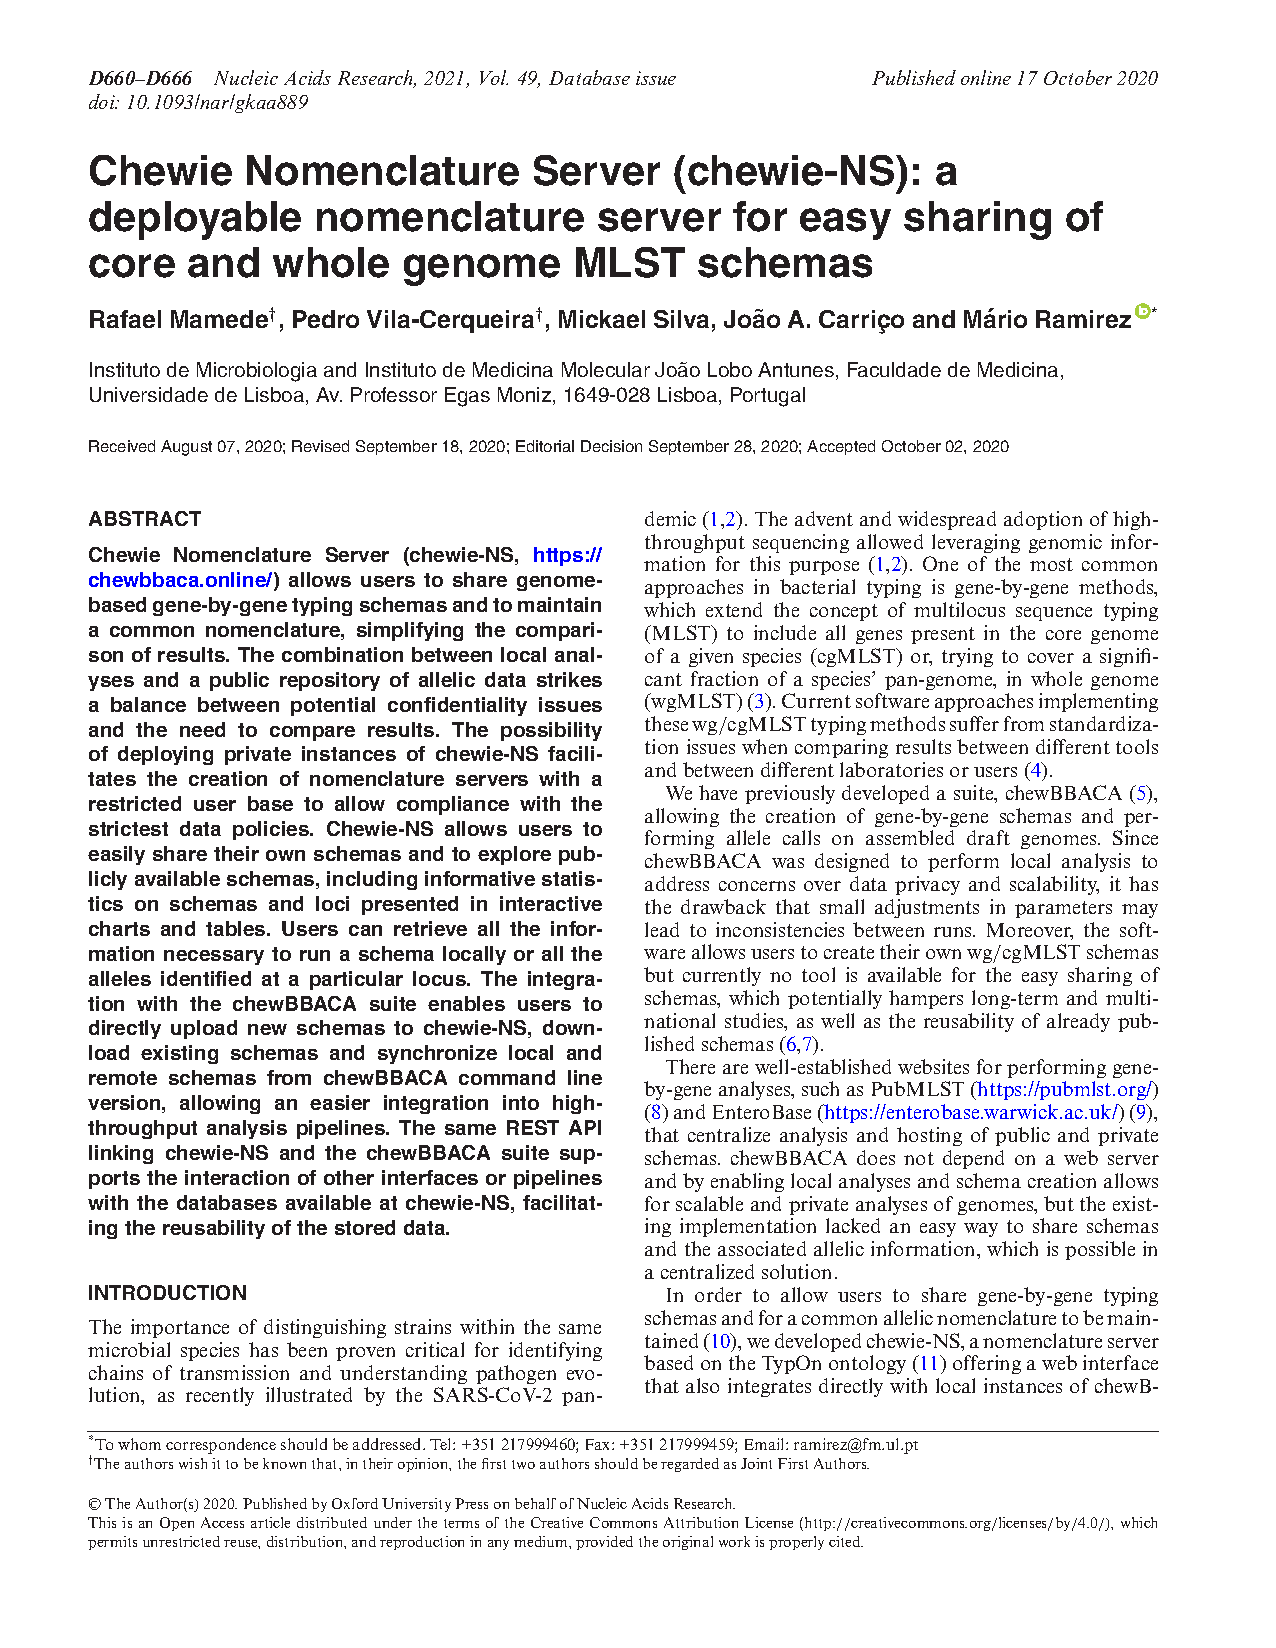
\includepdf[pages={1-}]{resources/papers/mamede2021.pdf}
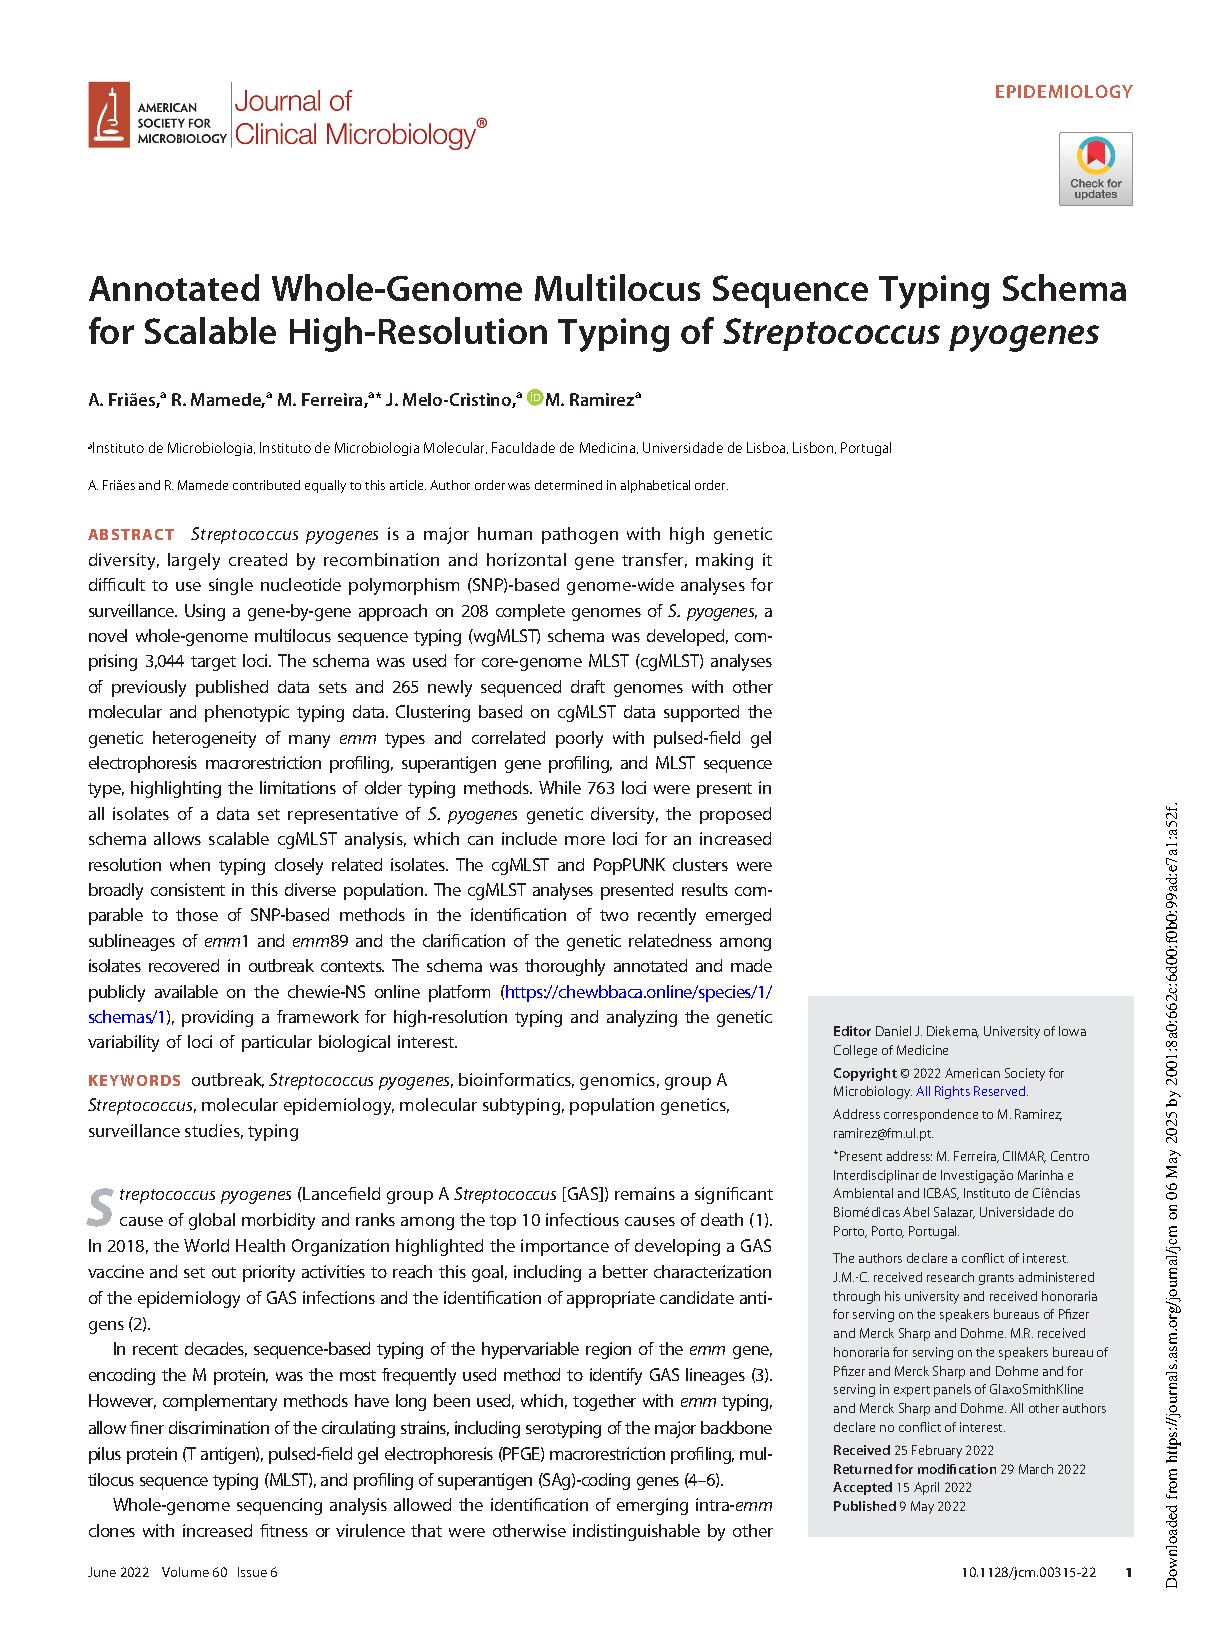
\includepdf[pages={1-}]{resources/papers/friaes2022.pdf}

\end{sloppy}
\end{document}
